\documentclass[a4paper,11pt]{book}
\usepackage[utf8]{inputenc}
\usepackage[spanish,es-tabla]{babel}
\usepackage[binary-units]{siunitx} % \num{} \SI{}
\usepackage{letltxmacro}
\LetLtxMacro{\svqty}{\qty}
\usepackage{physics}
\LetLtxMacro{\qty}{\svqty}
\newcommand*\diff{\mathop{}\!\mathrm{d}}
\usepackage{fullpage}
\usepackage{cite}
\usepackage[utf8]{inputenc}
\usepackage{a4wide}
\usepackage{url}
\usepackage{graphicx}
\usepackage{caption}
\usepackage{lmodern} % \fontsize{15}{18}\selectfont

\usepackage{ragged2e} %\justifying

\usepackage{float} % para que los gr\'aficos se queden en su lugar con [H]
\usepackage[labelformat=simple]{subcaption}
\renewcommand\thesubfigure{(\alph{subfigure})}

\usepackage{color}
\usepackage{colortbl} % para que funcione color en las tablas
\usepackage{amsmath} %para escribir funci\'on partida , matrices
\usepackage{amsthm} %para numerar definciones y teoremas
\usepackage[hidelinks]{hyperref} % para inlcuir links dentro del texto
\usepackage{tabu}
\usepackage{comment}
\usepackage{amsfonts} % \mathbb{N} -> conjunto de los n\'umeros naturales
\usepackage{enumerate}
\usepackage{listings}
\usepackage[colorinlistoftodos, textsize=small]{todonotes} % Para poner notas en el medio del texto!! No olvidar hacer.
\usepackage{framed} % Para encuadrar texto. \begin{framed}
\usepackage{csquotes} % Para citar texto \begin{displayquote}
\usepackage{epigraph} % Epigrafe  \epigraph{texto}{\textit{autor}}
\usepackage{authblk}
\usepackage{titlesec}
\usepackage{varioref}
\usepackage{bm} % \bm{\alpha} bold greek symbol
\usepackage{pdfpages} % \includepdf
\usepackage[makeroom]{cancel} % \cancel{} \bcancel{} etc
\usepackage{wrapfig} % \begin{wrapfigure} Pone figura al lado del texto
\usepackage{mdframed}
\usepackage{algorithm}
%\usepackage{quoting}
\usepackage{mathtools}
\usepackage{tikz}
\usepackage{paracol}
\usepackage{multirow}
% tikzlibrary.code.tex
%
% Copyright 2010-2011 by Laura Dietz
% Copyright 2012 by Jaakko Luttinen
%
% This file may be distributed and/or modified
%
% 1. under the LaTeX Project Public License and/or
% 2. under the GNU General Public License.
%
% See the files LICENSE_LPPL and LICENSE_GPL for more details.

% Load other libraries

%\newcommand{\vast}{\bBigg@{2.5}}
% newcommand{\Vast}{\bBigg@{14.5}}
% \usepackage{helvet}
% \renewcommand{\familydefault}{\sfdefault}

\usetikzlibrary{shapes}
\usetikzlibrary{fit}
\usetikzlibrary{chains}
\usetikzlibrary{arrows}

% Latent node
\tikzstyle{latent} = [circle,fill=white,draw=black,inner sep=1pt,
minimum size=20pt, font=\fontsize{10}{10}\selectfont, node distance=1]
% Observed node
\tikzstyle{obs} = [latent,fill=gray!25]
% Invisible node
\tikzstyle{invisible} = [latent,minimum size=0pt,color=white, opacity=0, node distance=0]
% Constant node
\tikzstyle{const} = [rectangle, inner sep=0pt, node distance=0.1]
%state
\tikzstyle{estado} = [latent,minimum size=8pt,node distance=0.4]
%action
\tikzstyle{accion} =[latent,circle,minimum size=5pt,fill=black,node distance=0.4]
\tikzstyle{fijo} =[latent,circle,minimum size=5pt,fill=black]


% Factor node
\tikzstyle{factor} = [rectangle, fill=black,minimum size=10pt, draw=black, inner
sep=0pt, node distance=1]
% Deterministic node
\tikzstyle{det} = [latent, rectangle]

% Plate node
\tikzstyle{plate} = [draw, rectangle, rounded corners, fit=#1]
% Invisible wrapper node
\tikzstyle{wrap} = [inner sep=0pt, fit=#1]
% Gate
\tikzstyle{gate} = [draw, rectangle, dashed, fit=#1]

% Caption node
\tikzstyle{caption} = [font=\footnotesize, node distance=0] %
\tikzstyle{plate caption} = [caption, node distance=0, inner sep=0pt,
below left=5pt and 0pt of #1.south east] %
\tikzstyle{factor caption} = [caption] %
\tikzstyle{every label} += [caption] %

\tikzset{>={triangle 45}}

%\pgfdeclarelayer{b}
%\pgfdeclarelayer{f}
%\pgfsetlayers{b,main,f}

% \factoredge [options] {inputs} {factors} {outputs}
\newcommand{\factoredge}[4][]{ %
  % Connect all nodes #2 to all nodes #4 via all factors #3.
  \foreach \f in {#3} { %
    \foreach \x in {#2} { %
      \path (\x) edge[-,#1] (\f) ; %
      %\draw[-,#1] (\x) edge[-] (\f) ; %
    } ;
    \foreach \y in {#4} { %
      \path (\f) edge[->,#1] (\y) ; %
      %\draw[->,#1] (\f) -- (\y) ; %
    } ;
  } ;
}

% \edge [options] {inputs} {outputs}
\newcommand{\edge}[3][]{ %
  % Connect all nodes #2 to all nodes #3.
  \foreach \x in {#2} { %
    \foreach \y in {#3} { %
      \path (\x) edge [->,#1] (\y) ;%
      %\draw[->,#1] (\x) -- (\y) ;%
    } ;
  } ;
}

% \factor [options] {name} {caption} {inputs} {outputs}
\newcommand{\factor}[5][]{ %
  % Draw the factor node. Use alias to allow empty names.
  \node[factor, label={[name=#2-caption]#3}, name=#2, #1,
  alias=#2-alias] {} ; %
  % Connect all inputs to outputs via this factor
  \factoredge {#4} {#2-alias} {#5} ; %
}

% \plate [options] {name} {fitlist} {caption}
\newcommand{\plate}[4][]{ %
  \node[wrap=#3] (#2-wrap) {}; %
  \node[plate caption=#2-wrap] (#2-caption) {#4}; %
  \node[plate=(#2-wrap)(#2-caption), #1] (#2) {}; %
}

% \gate [options] {name} {fitlist} {inputs}
\newcommand{\gate}[4][]{ %
  \node[gate=#3, name=#2, #1, alias=#2-alias] {}; %
  \foreach \x in {#4} { %
    \draw [-*,thick] (\x) -- (#2-alias); %
  } ;%
}

% \vgate {name} {fitlist-left} {caption-left} {fitlist-right}
% {caption-right} {inputs}
\newcommand{\vgate}[6]{ %
  % Wrap the left and right parts
  \node[wrap=#2] (#1-left) {}; %
  \node[wrap=#4] (#1-right) {}; %
  % Draw the gate
  \node[gate=(#1-left)(#1-right)] (#1) {}; %
  % Add captions
  \node[caption, below left=of #1.north ] (#1-left-caption)
  {#3}; %
  \node[caption, below right=of #1.north ] (#1-right-caption)
  {#5}; %
  % Draw middle separation
  \draw [-, dashed] (#1.north) -- (#1.south); %
  % Draw inputs
  \foreach \x in {#6} { %
    \draw [-*,thick] (\x) -- (#1); %
  } ;%
}

% \hgate {name} {fitlist-top} {caption-top} {fitlist-bottom}
% {caption-bottom} {inputs}
\newcommand{\hgate}[6]{ %
  % Wrap the left and right parts
  \node[wrap=#2] (#1-top) {}; %
  \node[wrap=#4] (#1-bottom) {}; %
  % Draw the gate
  \node[gate=(#1-top)(#1-bottom)] (#1) {}; %
  % Add captions
  \node[caption, above right=of #1.west ] (#1-top-caption)
  {#3}; %
  \node[caption, below right=of #1.west ] (#1-bottom-caption)
  {#5}; %
  % Draw middle separation
  \draw [-, dashed] (#1.west) -- (#1.east); %
  % Draw inputs
  \foreach \x in {#6} { %
    \draw [-*,thick] (\x) -- (#1); %
  } ;%
}


\allowdisplaybreaks %break equations



\newcommand\Wider[2][3em]{%
\makebox[\linewidth][c]{%
  \begin{minipage}{\dimexpr\textwidth+#1\relax}
  \raggedright#2
  \end{minipage}%
  }%
}

%

% \usepackage[rawfloats]{floatrow}
% \DeclareMarginSet{hangboth}{\setfloatmargins*{\hskip-4cm}{\hskip-4cm}}

%

\tikzset{
every picture/.append style={
  execute at begin picture={\deactivatequoting},
  execute at end picture={\activatequoting}
  }
}

%%%%%% Para no numerar los prefacios, y todo lo que viene antes del capitulo 1. Coimenzar con \frontmatter y volver a abrir con \mainmatter
\makeatletter
\renewcommand{\frontmatter}{\cleardoublepage\@mainmatterfalse}
\renewcommand{\mainmatter}{\cleardoublepage\@mainmattertrue}
\makeatother
%%%%%%

\definecolor{julia}{rgb}{1, 0.5, 1}
\definecolor{python}{rgb}{1, 1, 0.5}
\definecolor{r}{rgb}{0.70, 0.80, 1}
\definecolor{all}{rgb}{0.85, 0.85, 0.85}
\definecolor{gray}{rgb}{0.5,0.5,0.5}
\newcommand{\gray}{\color{black!65}}


\usepackage{listings}
\lstset{
  aboveskip=3mm,
  belowskip=3mm,
  showstringspaces=true,
  columns=flexible,
  basicstyle={\footnotesize\ttfamily},
  breaklines=true,
  breakatwhitespace=true,
  tabsize=4,
  showlines=true
}

\hypersetup{
    colorlinks,
    linkcolor={black!50!black},
    citecolor={black!50!black},
    urlcolor={black!80!black}
}

\newcommand{\T}{Traducir. }
\newcommand{\vm}[1]{\mathbf{#1}}
\newcommand{\N}{\mathcal{N}}
\newcommand{\citel}[1]{\cite{#1}\label{#1}}
\newcommand\hfrac[2]{\genfrac{}{}{0pt}{}{#1}{#2}} %\frac{}{} sin la linea del medio

\newtheorem{midef}{Definition}
\newtheorem{miteo}{Theorem}
\newtheorem{mipropo}{Proposition}

\theoremstyle{definition}
\newtheorem{definition}{Definition}[section]
\newtheorem{theorem}{Theorem}[section]
\newtheorem{proposition}{Proposition}[section]

\newtheorem{conclution}{\en{Conclution}\es{Conclusi\'on}}%[section]
\newtheorem{objective}{\en{Objective}\es{Objetivo}}%[section]


%http://latexcolor.com/
\definecolor{azul}{rgb}{0.36, 0.54, 0.66}
\definecolor{rojo}{rgb}{0.7, 0.2, 0.116}
\definecolor{rojopiso}{rgb}{0.8, 0.25, 0.17}
\definecolor{verdeingles}{rgb}{0.12, 0.5, 0.17}
\definecolor{ubuntu}{rgb}{0.44, 0.16, 0.39}
\definecolor{debian}{rgb}{0.84, 0.04, 0.33}
\definecolor{dkgreen}{rgb}{0,0.6,0}
\definecolor{gray}{rgb}{0.5,0.5,0.5}
\definecolor{mauve}{rgb}{0.58,0,0.82}

\newif\ifen
\newif\ifes
\newcommand{\en}[1]{\ifen#1\fi}
\newcommand{\es}[1]{\ifes#1\fi}
\newcommand{\En}[1]{\ifen#1\fi}
\newcommand{\Es}[1]{\ifes#1\fi}

\estrue


\newcommand{\E}{\en{S}\es{E}}
\newcommand{\A}{\en{E}\es{A}}
\newcommand{\Ee}{\en{s}\es{e}}
\newcommand{\Aa}{\en{e}\es{a}}



% % % RENOMBRES
\newcommand{\TITULO}[0]{An\'alisis bayesiano del aprendizaje en comunidades de video juegos}
\newcommand{\TITULOen}[0]{Bayesian analysis of learning in video game communities}



%\title{\huge Creencias adaptativas, \\ cultura y aprendizaje social}
%%Inferencia bayesiana para el estudio del aprendizaje social en comunidades virtuales
\author{Gustavo Landfried}


\begin{document}

\deactivatequoting % Por incompatibilidad entre Babel spanish con > y <

\frontmatter
\pagenumbering{roman}

\begin{center}

\includegraphics[scale=.8]{../logofcen.pdf}

\medskip
UNIVERSIDAD DE BUENOS AIRES

Facultad de Ciencias Exactas y Naturales

Departamento de Computaci\'on


\vspace{3cm}

\textbf{\LARGE \TITULO}
% \textsc{}

\vspace{1cm}



Tesis presentada para optar al t\'itulo de Doctor de la \\
Universidad de Buenos Aires en el \'area Ciencias de la Computaci\'on

\vspace{2.5cm}

\textbf{Lic. Gustavo Andr\'es Landfried}

\end{center}

\vspace{2.5cm}

\noindent Director de tesis: Dr. Esteban Mocskos

\noindent Codirector de tesis: Dr. Diego Fern\'andez Slezak

\noindent Consejero de estudios: Dr. Hern\'an Melgratti \\

%\noindent Lugar de trabajo: Departamento de Computaci\'on, Facultad de Ciencias Exactas y Naturales % NO SE MENCIONA DEBIDO A QUE ES EL MISMO QUE EL CONSIGNADO EN EL PUNTO 1

\vspace{0.5cm}

\noindent Buenos Aires, Abril de 2022\\

\noindent Fecha de defensa: \\%13 de diciembre de 2018\\

\vspace{0.5cm}

\hspace*{0pt}\hfill Firma \hspace{2cm}
\thispagestyle{empty}
\newpage
%%%%%%%%%%%%% FIN CARATULA

\thispagestyle{empty}
\phantom{Pagina en blanco}
\newpage


\phantom{.}

\vspace{6cm}

\hfill  \scalebox{1.6}{El conocimiento emerge como la vida}

\newpage

\phantom{Pagina en blanco}

\newpage

\begin{center}
\Large \TITULO \normalsize \\[0.5cm]

\textbf{Resumen}
\end{center}

\small

Esta es una tesis en ciencias de la computaci\'on motivada por una pregunta antropol\'ogica.
Entender las propiedades de los sistemas de informaci\'on cultural es uno de los problemas fundamentales de la antropolog\'ia, relevante para las ciencias de la computaci\'on y la inteligencia artificial multi-agente: la sociedad puede ser vista como un sistema de procesamiento distribuido de informaci\'on, y la cultura como el emergente de su intercambio de informaci\'on.
Hasta ahora, las respuestas con mayor influencia para la antropolog\'ia se han propuesto a trav\'es de modelos matem\'aticos simples.
De all\'i surgieron, por ejemplo, las hip\'otesis de que la capacidad de acumulaci\'on cultural es proporcional al tama\~no efectivo de la poblaci\'on, y que estructuras con moderada conexi\'on favorecen la innovaci\'on cultural.
Si bien los resultados de estos modelos sirven para ganar intuici\'on de procesos complejos, sus resultados son analog\'ias que no est\'an destinadas a realizar predicciones y por lo tanto poseen una d\'ebil corroboraci\'on emp\'irica.

% Parrafo

En la \'ultima d\'ecada, las ciencias de la computaci\'on han tenido un impacto profundo en casi todas las disciplinas cient\'ificas, produciendo la emergencia de la ciencia de datos.
Esta tesis se enmarca en esta nueva forma de interdisciplina, que pone a prueba los m\'etodos computacionales en base al desempe\~no que tienen sobre datos reales.
Para ello, decidimos centrarnos en las comunidades de videojuegos en l\'inea debido a que ellas son un lugar privilegiado para estudiar c\'omo cambian las estrategias en el tiempo.
En el transcurso de la tesis, esta pregunta fue mutando hasta enfocarse en el estudio de los factores sociales que afectan el aprendizaje individual.
En este contexto nos propusimos responder las siguientes preguntas.
?`Cu\'al es la mejor forma de medir el aprendizaje de un individuo en el tiempo?
?`Cu\'al es la relaci\'on entre la formaci\'on de equipos y el aprendizaje individual a largo plazo?
?`Cu\'al es el efecto que la posici\'on topol\'ogica de un individuo en la red de intercambios din\'amica tiene sobre el aprendizaje individual?

% Parrafo

Si bien el aprendizaje autom\'atico funciona muy bien en ciertos contextos, puede colapsar si los datos se desv\'ian un poco de lo que el modelo est\'a acostumbrado.
Las ciencias, sin embargo, buscan verdades con validez universal.
Para no mentir en contextos de incertidumbre debemos no afirmar m\'as de lo que sabemos, sin dejar de decir todo lo que s\'i sabemos.
Por ello, la aplicaci\'on estricta de las reglas de la probabilidad (enfoque bayesiano) es el m\'etodo con el que se fundamentan las verdades en contextos de incertidumbre.
Al evaluar hip\'otesis mutuamente contradictorias (A y no A) la sorpresa, \'unica fuente de informaci\'on, act\'ua como filtro de las creencias previas, permitiendo no decir m\'as de lo que se sabe incorporando toda la informaci\'on disponible (maximiza incertidumbre compatible con los datos).
Si bien hubieron algunas partes de la tesis que no pudimos evaluar todo el espacio de hip\'otesis, hicimos un esfuerzo por ajustarnos a este ideal.

% Parrafo

En el primer trabajo usamos el modelo bayesiano de habilidad m\'as utilizado en la industria del video juego para estudiar una comunidad en el que las personas pod\'ian jugar individualmente o en equipos.
All\'i encontramos que jugar en equipo est\'a asociado a mayor aprendizaje a largo plazo, y que mantener un equipo estable est\'a asociado a mayor velocidad de aprendizaje.
En el segundo trabajo, replicamos el estimador de habilidad y descubrimos que ninguno de los modelos disponibles en aquel momento pod\'ia obtener estimaciones iniciales fiables ni garantizaban comparabilidad en el tiempo debido a una incorrecta propagaci\'on de la informaci\'on hist\'orica, solo en la direcci\'on del pasado hacia el futuro.
En este contexto, implementamos un modelo (disponible hoy en Julia, Python y R) que al propagar correctamente la informaci\'on hist\'orica es capaz de proporcionar estimaciones con baja incertidumbre en todo momento, asegurando la comparabilidad hist\'orica.
En un tercer trabajo, estudiamos la evoluci\'on de una red de partidas en el juego de Go durante un periodo de ocho a\~nos y encontramos, con el nuevo estimador, que la posici\'on de los individuos en la red tiene un efecto de segundo orden sobre el aprendizaje en los personas que est\'an en el medio del proceso de aprendizaje, ausente entre novatas y expertas.

\vspace{0.1cm}

\noindent \textbf{Palabras claves}: Ciencias Sociales Computacionales, Inferencia bayesiana, Cultura, Habilidad, Aprendizaje, Comunidades virtuales, Videojuegos


\newpage


\begin{center}
\Large \TITULOen \normalsize \\[0.5cm]

\textbf{Abstract}
\end{center}


This thesis in computer science is motivated by an anthropological question.
One of the fundamental problems of anthropology, relevant to computer science and multi-agent artificial intelligence, is to understand the properties of cultural information systems.
Society can be viewed as a distributed information processing system, and culture as the emergent result of information exchange.
Until now, the most influential answers to these questions in anthropology have been proposed using simple mathematical models.
They have led, for example, to the hypotheses that the capacity for cultural accumulation is proportional to the effective population size, and that moderately connected structures favor cultural innovation.
While the results of these models serve to gain intuition of complex processes, their results are analogies not intended to make predictions and therefore have weak empirical support.

% Parrafo

In the last decade, computer science has had a profound impact on almost all scientific disciplines, producing the emergence of data science.
This thesis is part of this new form of interdiscipline, which evaluates computational methods based on their performance on real data.
To this end, we decided to focus on online gaming communities because they are a valuable source of informnation to study how strategies change over time.
In the course of the thesis, this question gradually evolved into the study of the social factors that affect individual learning.
In this context, we set out to answer the following questions:
What is the best way to measure individual's learning curves over time?
What is the relationship between team formation and long-term individual learning?
What is the effect that an individual's topological position in the dynamic exchange network has on individual learning?

% Parrafo

While machine learning works very well in certain contexts, it can crash if the data deviates a bit from what the model is accustomed to.
The sciences, however, seek truths with universal validity.
To avoid lying in contexts of uncertainty, we must not assert more than we know, without saying less.
Therefore, the strict application of the rules of probability (Bayesian approach) is the method by which truths are grounded in contexts of uncertainty.
When evaluating mutually contradictory hypotheses (A and not A) surprise, the only source of information, acts as the filter of prior beliefs, allowing not to say more than what is known by incorporating all available information (maximizes uncertainty compatible with the data).
Although there were some parts of the thesis that we could not evaluate the entire hypothesis space, we made an effort to adhere to this ideal.

% Parrafo

In the first paper we used the Bayesian skill model most commonly used in the gaming industry to study a community in which people could play individually or in teams.
There we find that playing in teams is associated with higher long-term learning, and that maintaining a stable teammate is associated with faster learning.
In the second paper, we replicated the skill estimator and discovered that none of the models available at that time could obtain reliable initial estimates nor did they guarantee comparability over time due to an incorrect propagation of historical information, only in the direction from the past to the future.
In this context, we implemented a model (now public in Julia, Python and R) that, by correctly propagating historical information, is able to provide estimates with low uncertainty at all times, ensuring historical comparability.
In a third paper, we studied the evolution of a network of games in the game of Go over a period of eight years and we found, thanks to the new estimator, that the position of individuals in the network has a second-order effect on learning for individuals who are in the middle of the learning process, absent among novices and experts.
%
\vspace{0.1cm}

\noindent \textbf{Keywords}: Computational social science, Bayesian inference, Culture, Skill, Learning, Virtual communities, Video games

\normalsize

\tableofcontents

\newpage

\vfill

\pagenumbering{arabic}

\normalsize

\chapter*{Agradecimientos: soy porque son.}

El primer derecho es formar parte de una comunidad.
%
Hay que saber dar y recibir con dicha y agradecimiento porque la vida es la uni\'on de muchos seres y fuerzas, dice el \'ultimo de los 13 principios aymaras del buen vivir (\emph{Suma Chura\~na, Suma Katuka\~na}).
%
Nuestra propia vida depende al menos de 4 niveles de cooperaci\'on para sobrevivir: la c\'elula con la mitocondria, el organismo multicelular, la sociedad y el ecosistema.
%
No hay m\'erito individual, el m\'erito siempre es colectivo.
%
De quienes ya no est\'an.
%
De quienes no recordamos.
%
De quienes nunca conocimos.
%
Hacia ellas quedar\'a mi deuda, que espero compensar con quienes tuve y tengo cerca d\'ia a d\'ia.
%
A mi compa\~nera Laura, que me nutri\'o en todos los aspectos de la vida, d\'ia tras d\'ia, desde el mero sue\~no hasta la realidad concreta, todo el m\'erito es tuyo. Siempre merec\'es m\'as de lo que puedo dar.
%
A mi madre Adriana, que me dio la vida y me hizo ser quien soy, quien no puedo dejar de ser aunque quisiera, todo el m\'erito es tuyo. Siempre merec\'es m\'as de lo que puedo dar.
%
A mi director Esteban, que me abri\'o todas las puertas y me dej\'o ser y hacer a pesar de mis locuras y errores, todo el m\'erito es tuyo. Espero por lo menos no quedar en deuda con vos.
%
A mi hermana Carolina y mi hermano Hern\'an, con qui\'en compart\'i intensamente los primeros a\~nos de mi vida, gracias, sin su est\'imulo no me imagino como ser\'ia mi presente.
%
A mis sobrinos Delfina e Ignacio, a quienes les deseo que se les abra el mundo y vivan en compa\~n\'ia, salud y bienestar.
%
A mi padre Alberto que me cuid\'o con el amor de un abuelo.
%
A la madre de mi madre, la abuela Pichi, por darme toda una familia que le dio vida a mi coraz\'on.
%
A la abuela de mi abuela, y a la mitad de la poblaci\'on argentina, a quienes le impidieron hablar su lengua materna.
%
A mis referentes intelectuales Rita, Enrique, Juan, Shara, Edwin de quienes obtuve las principales respuestas.
%
A los responsables de esta locura, el Grupo Antropocaos, a Ram\'on, Diego, Sergio, Jorge, Mora, Alejandro, Laura y toda la banda.
%
A mis compa\~neros doctorales de oficina antes de la pandemia, Maxi, David, Emmanuel y Rodolfo, adem\'as de ser un gran apoyo, disfrut\'e mucho compartir con ustedes.
%
A los profesores del Laboratorio de Inteligencia Artificial Aplicada, Diego, Agust\'in, Luciana y Juanka, por integrarme en un hermoso grupo humano.
%
A mi codirector Diego nuevamente, que estuvo presente para darme el primer impulso.
%
A mis contempor\'aneos Edgard, Facundo, Juanma, Riera, Bruno, March, Lara, Jazm\'in, Gast\'on, Marcos, Daniela, Ramiro, Brusco, Lao, con quienes pude compartir.
%
A mis estudiantes Macarena, Tob\'ias, Mart\'in, Agust\'in, Gustavo, gracias por ayudarme a ser mejor.
%
A todo el Grupo Antropocaos, por se\~nalarme el camino.
%
A todo el Departamento de Computaci\'on y el Instituto de Ciencias de la Computaci\'on, sus autoridades, sus profesores, sus docentes, a A\'ida, Paula y Alejandro, por haberme acogido en su comunidad.
%
A las y los consejeros de la Facultad de Ciencias Exactas y Naturales, por asumir la responsabilidad de construir d\'ia a d\'ia una instituci\'on p\'ublica, de excelencia, din\'amica, popular, inclusiva y comprometida con la realidad nacional.
%
A quienes dan la vida en la pol\'itica por un pa\'is mejor, en particular a Cristina por haber fortalecido el financiamiento en ciencia que me permiti\'o hacer realidad este proyecto.









\mainmatter

\chapter{Introducci\'on} \label{ch:evo}

\section{Motivación}

El aprendizaje es una forma de plasticidad conductual que permite a los individuos ajustar su comportamiento a las condiciones ambientales locales.
%
Cuando el aprendizaje puede ser transmitido socialmente (a partir de la observaci\'on de otros o de la interacci\'on con ellos), aparece un sistema de informaci\'on no-gen\'etico denominado cultura que se transmite de un individuo a otro, entre poblaciones y a lo largo de las generaciones.
%
Muchos animales son capaces de transmitir informaci\'on no-gen\'etica y producir tradiciones simples persistentes en el tiempo.
%
En algunos casos, como las ballenas, delfines, primates y aves, las tradiciones pueden ser incluso bastante complejas.
%
Por ejemplo, los cantos de las aves, sus estrategias de b\'usqueda de alimento, e incluso las rutas migratorias son comportamientos que se transmiten por v\'ia social, produciendo la formaci\'on de culturas locales~\cite{aplin2022-birdsCulture}.
%
Sin embargo, todas ellas son manifiestamente m\'as simples que la cultura humana~\cite{boyd1996-whyCultureIsCommon}.

% Parrafo

Lo singular de la especie humana es la capacidad de acumular adaptaciones culturales en el tiempo, modificaciones sucesivas que van produciendo un sistema de informaci\'on cultural inimaginablemente complejo~\cite{Tomasello1993, Boyd2011}.
%
Si bien el aprendizaje humano ocurre en los cuerpos biol\'ogicos, es parte de un fen\'omeno poblacional que emerge como consecuencia del intercambio de informaci\'on entre individuos.
%
La cultura humana es la informaci\'on transmitida por v\'ia comportamental, y la sociedad humana el sistema distribuido de almacenamiento y procesamiento~\cite{Derex2020}.

% Parrafo

Comprender algunas de las relaciones que vinculan el nivel poblacional (como la din\'amica y estructura de la red de intercambios de informaci\'on cultural) con el nivel individual (el aprendizaje efectivo que se produce en cada uno), es la pregunta general que intentamos explorar en esta tesis.
%
Surgen r\'apidamente muchos conceptos y muchas definiciones a distinguir.
%
Por ejemplo, ?`hay una forma \'optima de aprender en contextos de incertidumbre?
%
Este problema lo tratamos en el cap\'itulo~\ref{ch:Incertidumbre}, donde discutimos: las reglas de razonamiento de las ciencias emp\'iricas, el m\'etodo de evaluaci\'on de sistemas de comunicaci\'on con la realidad, y una aplicaci\'on de inter\'es para la tesis (los modelos de estimaci\'on de habilidad en el tiempo).

% Parrafo

El concepto de aprendizaje tiene diferentes acepciones.
%
Los modelos de estimaci\'on de habilidad que se utilizan para medir el desempe\~no de los individuos en la industria del videojuego difiere del concepto de aprendizaje que se establece desde un punto de vista biol\'ogico, cognitivo o social.
%
En pocas palabras, los modelos utilizados en la industria del videojuego (as\'i como gran parte de las evaluaciones internacionales de los sistemas educativos) son instrumentos que predicen la probabilidad de \'exito o fracaso.
%
En definitiva, el modelo causal sobre el que se basan sus estimaciones (ver detalles en cap\'itulo~\ref{ch:Incertidumbre} y \ref{ch:ttt}) es una simplificaci\'on extrema de la realidad causal que gobierna los procesos de aprendizaje humano.

% Parrafo

Cuando hacemos referencia a modelos causales nos estamos refiriendo a modelos que se resuelven aplicando las reglas de la probabilidad y que cumplen con la definici\'on probabil\'istica de causalidad (ver definici\'on precisa en la secci\'on~\ref{}).
%\todo[inline]{Arriba te qued\'o una referencia sin completar}
%
Idealmente quisi\'eramos tener teor\'ias causales, o sistemas de modelos causales, que incluyan todos los elementos relevantes de la realidad causal estudiada.
%
Y quisi\'eramos adem\'as que el efecto causal se derive de la correcta evaluaci\'on de las teor\'ias causales alternativas.
%
Sin embargo, en la actualidad no existe tal cosa.

% Parrafo

Esta tesis se destaca, en particular, por haber realizado la primera implementaci\'on del modelo de estimaci\'on de habilidad estado del arte en la industria del video juego, que si bien ya estaba especificado matem\'aticamente, no se encontraba todav\'ia disponible como paquete para ser utilizado en alg\'un lenguaje de programaci\'on.
%
La novedad no es tanto el modelo causal de base (que se ve en detalle en el cap\'itulo~\ref{ch:Incertidumbre} y \ref{ch:ttt}), el cual es tan simple como en los anteriores.
%
La mejora que introduce proviene de integrar todos los modelos causales de base (los eventos donde ocurren los \'exitos o los fracasos) en una \'unica red causal hist\'orica (la habilidad del pasado es una causa de la habilidad del presente).
%
Esto permite propagar la informaci\'on por toda la red, obteniendo as\'i estimaciones con menor incertidumbre en todas las series temporales.

% Parrafo

Este modesto avance da cuenta de la dificultad que existe en el campo de los estudios del aprendizaje para proponer y evaluar modelos causales capaces de integrar los diversos elementos de inter\'es que forman parte de nuestros objetos reales de estudio.
%
Por ese motivo, cuando en los cap\'itulos~\ref{ch:team} y \ref{ch:topo} exploramos en bases de datos reales el efecto que algunos factores sociales tienen sobre el aprendizaje de los individuos, nos vimos obligados a recurrir a diversas heur\'isticas estad\'isticas que si bien arrojan luz, no garantizan conclusiones definitivas.
%
Solo recientemente, en el trascurso del doctorado apareci\'o quiz\'as el primer modelo causal (en el sentido probabil\'istico del t\'ermino) capaz de integrar diversos elementos que son espec\'ificos al problema de estudio~\cite{minka2018-trueskill2}.
%
Este modelo es una extensi\'on de nuestra implementaci\'on, y todav\'ia no se encuentra disponible como paquete en ning\'un lenguaje de programaci\'on.

% Parrafo

Durante el transcurso del doctorado, investigadores que han sido protagonistas del desarrollo de la teor\'ia de la evoluci\'on moderna han comenzado a se\~nalar el isomorfismo que existe entre las teor\'ia de la evoluci\'on y la inferencia bayesiana~\cite{czegel2019-bayesianEvolution, czegel2022-bayesDarwin} (el modelo est\'andar de evoluci\'on conocido como \emph{replicator dynamic} \cite{taylor1978-replicatorDynamic} es estructuralmente equivalente al teorema de Bayes~\cite{harper2009-replicatorAsInference,shalizi2009-replicatorAsInference}).
%
En el cap\'itulo~\ref{ch:epistemico} discutimos algunas de las propiedades que se derivan de la funci\'on de costo compartida por las teor\'ias de la probabilidad y de la evoluci\'on.
%
Luego de haber extendido la frontera de los modelos de estimaci\'on de habilidad disponibles en los lenguajes de programaci\'on, y haberlo utilizado para explorar casos reales, finalizamos la tesis con esta reflexi\'on general respecto de la naturaleza de los aprendizajes epist\'emicos (de las hip\'otesis) y evolutivos (de la vida).

% Parrafo

\subsection{Aprendizaje humano}

El aprendizaje se define como un cambio persistente en las representaciones o asociaciones mentales como resultado de la experiencia individual o social, y es observable a trav\'es del comportamiento.
%
Los comportamientos observables pueden ser: la aparici\'on de una nueva habilidad (por ejemplo, aprender a contar); cambios en la frecuencia de un comportamiento existente (por ejemplo, cooperar m\'as regularmente con otros); modificar la velocidad o eficiencia de un comportamiento existente (en ajedrez, el tiempo de mover la pieza); cambios en la intensidad de un comportamiento existente (en deporte, obtener victorias cada vez m\'as holgadas); modificar la complejidad de un comportamiento existente (por ejemplo, debatir un tema con mayor profundidad conceptual); responder de forma diferente a un est\'imulo concreto (en psicolog\'ia, la respuesta al miedo)~\cite{Ormrod2017}.

% Parrafo

Aunque los investigadores pueden diferir en sus opiniones sobre la mejor manera de definir el aprendizaje y determinar cu\'ando se ha producido, existe una coincidencia respecto de que para estudiar el aprendizaje es necesario observar las modificaciones en el comportamiento de modo tal de poder inferir aquellos cambios persistentes que van desarrollando los individuos a trav\'es de la experiencia.
%
A finales del siglo 19, las perspectivas dominantes en psicolog\'ia eran el \emph{estructuralismo} y el \emph{funcionalismo}.
%
Aunque ellas difer\'ian considerablemente entre s\'i, compart\'ian una debilidad com\'un: el principal medio para investigar el aprendizaje y otros fen\'omenos psicol\'ogicos era un m\'etodo llamado \emph{``introspecci\'on''} basado en la auto-percepci\'on del paciente~\cite{Ormrod2017}.

% Parrafo

A comienzos del siglo 20, una corriente comienza a proponer m\'etodos de estudio basado en las conductas de las personas (respuestas) y los cambios ambientales (est\'imulos) que preceden y siguen a esas respuestas.
%
Desde entonces, muchos psic\'ologos han intentado describir y comprender el aprendizaje y la conducta principalmente a trav\'es del an\'alisis de las relaciones est\'imulo-respuesta.
%
Esta escuela fue denominada \emph{conductista} y, en su primera etapa, cre\'ia que el aprendizaje s\'olo se produc\'ia por experiencia individual.
%
Alrededor de 1940, algunos psic\'ologos propusieron una perspectiva alternativa, la \emph{teor\'ia del aprendizaje social}, que se centraba en la transmisi\'on de informaci\'on entre las personas~\cite{Ormrod2017}.
%
Ambas corrientes se desarrollaron principalmente en Estados Unidos.

% Parrafo

Con el tiempo, los te\'oricos del aprendizaje social fueron incorporando el an\'alisis de los procesos mentales (o cognitivos) a los estudios del aprendizaje.
%
Sin embargo, ni la cognici\'on ni el comportamiento permit\'ian determinar las caracter\'isticas distintivas del aprendizaje humano.
%
?`Cu\'ales son, entonces, las propiedades particulares del aprendizaje humano?
%
La incre\'ible flexibilidad lingü\'istica de los humanos permite una acumulaci\'on de conocimientos a trav\'es de las generaciones mucho m\'as compleja que la que logran otras especies.

% Parrafo

En las \'ultimas d\'ecadas, la psicolog\'ia ha comenzado a incorporar los an\'alisis de las interacciones sociales y la transmisi\'on cultural en sus estudios sobre los procesos del aprendizaje humano.
%
La etiqueta m\'as utilizada es la de \emph{teor\'ia sociocultural}, pero en t\'erminos m\'as generales podemos pensar en ellas como teor\'ias contextuales~\cite{Ormrod2017}.
%
Los seres humanos crecen y se desarrollan en entornos culturales, por lo que la din\'amica de los sistemas de intercambio de informaci\'on cultural afectan directamente nuestros procesos de aprendizaje individual.

% Parrafo

En la historia reciente, la intensificaci\'on de la interconexi\'on global a partir del uso de energ\'ias f\'osiles en el siglo 19 y el desarrollo de las comunicaciones electr\'onicas durante el siglo 20 han tenido produndas consecuencias para el desarrollo de la ciencia moderna.
%
En la actualidad, la adopci\'on de los \emph{smartphones} como dispositivos de comunicaci\'on instant\'anea, est\'a teniendo consecuencias concretas sobre los procesos de aprendizaje colectivo e individual que aun desconocemos.

\subsection{La cultura}

En la historia del ser humano, la transici\'on cultural tuvo un efecto positivo radical para la especie.
%
Hubo un per\'iodo en el que se enfrent\'o un grave peligro de extinci\'on, lo que se evidencia en la baja diversidad del genoma humano respecto, incluso, de los hom\'inidos m\'as cercanos~\cite{Hrdy2009}.
%
Pero cuando el conocimiento, que antes deb\'ia ser redescubierto individualmente, pas\'o a ser un recurso com\'un transmitido de generaci\'on en generaci\'on, la especie humana comenz\'o a ser capaz de ocupar todos los nichos ecol\'ogicos de la tierra como ning\'un otro vertebrado terrestre lo hab\'ia logrado antes.
%
Debido a que la cultura es un sistema de informaci\'on, a largo de la evoluci\'on humana fueron emergiendo naturalmente diversos mecanismos de comunicaci\'on, cada uno de los cuales impactaron directamente sobre la tasa de aprendizaje de nuestra especie y sobre nuestras tasas individuales de aprendizaje.

% Parafo

Antes del surgimiento de los humanos anat\'omicamente modernos (masa cerebral actual) y de los humanos conductualmente modernos (lenguaje), surgi\'o en \'Africa una linaje emocionalmente moderno, con capacidades para el entendimiento mutuo~\cite{Hrdy2020}.
%
A diferencia de las especies m\'as cercanas, nuestros ancestros comenzaron a desarrollar un tipo de crianza cooperativa que favoreci\'o la selecci\'on de j\'ovenes con capacidades para comunicar y comprender las intenciones de los dem\'as~\cite{Hrdy2020}.
%
A trav\'es de rondas repetidas de co-evoluci\'on gen\'etico-cultural, se fueron desarrollando las caracter\'isticas biol\'ogicas, cognitivas y sociales que permiten hoy a los humanos aprender y transmitir rasgos culturales complejos a trav\'es de las generaciones~\cite{Jones2011}.

%

Esta capacidad biol\'ogica para la comprensi\'on mutua y la imitaci\'on (\emph{aprendizaje social}) dio inicio a este proceso inter-generacional de acumulaci\'on de innovaciones, que ha sido tan exitoso para la adaptaci\'on humana.
%
Lo que antes deb\'ia ser redescubierto una y otra vez mediante la costosa experiencia individual, ahora pod\'ia ser transmitido a la siguiente generaci\'on.
%
Como consecuencia, nadie individualmente es capaz de redescubrir en un per\'iodo de vida ni siquiera los repertorios culturales de las sociedades cazadoras recolectoras actuales consideradas m\'as simples.

% Parrafo

Otra importante modificaci\'on en el sistema de intercambio de informaci\'on cultural comenz\'o hace 10 mil a\~nos con el surgimiento independiente de la agricultura en seis regiones distintas del mundo (\'Africa subsahariana, Oriente medio, China, Ocean\'ia, Am\'erica del Norte y Am\'erica del Sur).
%
El aumento progresivo de la poblaci\'on y el surgimiento de la escritura intensificaron los procesos de acumulaci\'on cultural, haciendo de estas regiones los principales centros tecnol\'ogicos de la humanidad.
%
Para el a\~no 1400 en el mundo florec\'ian de sociedades pr\'osperas: China llevaba 2 milenios siendo el principal centro productivo y tecnol\'ogico del mundo; en el mundo \'Arabe se comerciaban estos productos desde el oc\'eano Atl\'antico en Espa\~na, hasta el oc\'eano Pac\'ifico en las Filipinas; el oc\'eano Pac\'ifico estaba totalmente ocupado, y ya se hab\'ian producido intercambios entre Ocean\'ia y Am\'erica del Sur; y en el jard\'in de la diversidad gen\'etica y cultural humana, \'Africa subsahariana, se desarrollaba entre otras, la sociedad Bantu.


% Parrafo

As\'i como los sistemas de comunicaci\'on favorecen los proceso de aprendizaje social y acumulaci\'on cultural, el aislamiento est\'a asociado a p\'erdidas masivas de informaci\'on cultural.
%
El ejemplo paradigm\'atico es el aislamiento total que ocurri\'o con la separaci\'on de Tasmania del continente Australiano por la subida del nivel del mar a comienzos del Holoceno~\cite{Henrich2004}.
%
La evidencia indica que las sociedades que permanecieron en la isla de Tasmania perdieron gran parte de su cultura tecnol\'ogica.
%
De forma similar, el aislamiento de Europa occidental del sistema mundo luego de la masiva destrucci\'on de la diversidad cultural al interior del imperio Romano condujo a un largo proceso de involuci\'on cultural y de violencia interna conocido como Edad Media~\cite{dussel2004}.

% Parrafo

Estas observaciones sugieren que el aprendizaje humano es una propiedad poblacional.
%
Si bien se han propuesto muchas causas internas para explicar la prosperidad actual de Europa occidental\footnote{La ``\'etica protestante'' de Max Weber~\cite{weber1905-eticaProtestante}, la ``mentalidad burguesa'' de Jos\'e Luis Romero~\cite{romero1967-revolucionBurguesa}, o m\'as recientemente el ``sistema de parentesco'' de Joseph Henrich~\cite{henrich2020-weirdest}}, ninguna de ellas puede responder la paradoja de c\'omo una sociedad como la feudal, sumida en un proceso de involuci\'on cultural \'unico, pudo generar de repente el extraordinario desarrollo cient\'ifico y t\'ecnico de la modernidad.
%
Nada de esto resulta extra\~no cuando se consideran los eventos globales: las enfermedades transmitidas por los exploradores feudales que eliminaron al menos a 2/3 de la poblaci\'on americana; y el giro geopol\'itico que se produce a partir de que en 1546 los exploradores feudales descubren la monta\~na de plata de Potos\'i, metal que China hab\'ia incorporado recientemente como una de sus monedas oficiales~\cite{dussel2017}.

% Parrafo

Sin embargo, no todo aumento de la interconexi\'on es positivo.
%
M\'as de dos siglos despu\'es del acceso a la plata americana, Europa occidental segu\'ia consumiendo m\'as productos asi\'aticos de los que pod\'ia exportar a Asia.
%
Luego de la derrota de China contra el narcotr\'afico brit\'anico (en el siglo 19), Europa occidental comienza la ocupaci\'on de \'Africa y de otros territorios no colonizados.
%
Si bien es una \'epoca de avances cient\'ificos y tecnol\'ogicos por un lado, es al mismo tiempo la era de genocidios y masiva p\'erdida de diversidad cultural global.
%
A pesar de todos los avances, la ciencia metropolitana no es capaz de compensar la p\'erdida de los conocimientos milenarios, y la crisis ecol\'ogica que no deja de profundizarse.

% Parrafo

El aprendizaje individual tambi\'en se ve especialmente afectado por la din\'amica de las ``redes culturales''.
%
Estudios recientes han cuestionado la hip\'otesis de que todo lo que maximice el flujo de informaci\'on cultural deber\'ia repercutir positivamente~\cite{Derex2020}.
%
La hip\'otesis afirma que las redes totalmente conectadas producen una homogeneizaci\'on cultural que reduce las posibilidades de innovaci\'on, mientras que las redes fragmentadas tienden a perder variantes culturales complejas con el tiempo~\cite{padilla2022-interconnectivity,derex2018-divideAndConquer,Creanza2017}.
%
Pero son pocos los estudios que ponen a prueba estas hip\'otesis en datos del mundo real~\cite{migliano2017-hunterGathererNetwork, Derex2020}.

% Parrafo


\subsection{Objetivo}

Nuestro plan de tesis tiene como objetivo explorar los efectos que diversos factores sociales tienen sobre el aprendizaje individual.
%
Una de las razones por las que es dif\'icil evaluar el efecto que las interacciones sociales (su contexto, din\'amica y estructura) tiene sobre el aprendizaje individual es la necesidad de registrar los contactos a nivel individual, lo que suele ser dif\'icil en estudios antropol\'ogicos cl\'asicos.
%
Para evaluar algunas de estas hip\'otesis, decidimos estudiar en el tiempo la evoluci\'on de la habilidad al interior de comunidades de jugadores en l\'inea.

% Parrafo

Si bien el estudio de las comunidades virtuales impone alguna limitaciones, ellas ofrecen nuevos horizontes en la investigaci\'on cient\'ifica sobre comportamientos sociales pues re\'unen, al mismo tiempo, la posibilidad de estudiar poblaciones suficientemente grandes con un alto nivel de detalle.
%
Ninguna de las metodolog\'ias cl\'asicas de las ciencias sociales (censo, encuesta, etnograf\'ia) ofrecen simult\'aneamente ambos niveles de an\'alisis.
%
En particular, los videojuegos aparecen como un lugar privilegiado para estudiar c\'omo las personas aprenden en diversos contextos culturales.

% Parrafo

En la \'ultima d\'ecada se han desarrollado investigaciones sobre comportamientos humanos basadas en datos obtenidos de comunidades virtuales.
%
Durante el transcurso del doctorado emergi\'o con fuerza una \'area conocida como \textbf{Ciencias Sociales Computacionales}~\cite{Lazer2009,Lazer2020}, que tiene en la actualidad reconocimiento tanto en institutos de primer nivel de ciencias de la computaci\'on como en los gigantes tecnol\'ogicos relacionados a la industria del software.
%
En antropolog\'ia se han llevado adelante estudios sobre la din\'amica de copia y modificaci\'on de c\'odigo en competencias de programaci\'on en l\'inea~\cite{miu2018-cumulativeCultureOnlineProgrammingContests}.
%
En computaci\'on se ha estudiado el efecto del miedo sobre la habilidad en una base de datos de ajedrez r\'apido~\cite{slezak2012-doNotFearYourOpponent}.

% Parrafo

Una de las ventajas del estudio de las comunidades virtuales es el intercambio de conocimientos entre los participantes.
%
Esto crea oportunidades para estudiar no solo el aprendizaje individual, sino tambi\'en c\'omo se construye el conocimiento de manera colaborativa en entornos en l\'inea.
%
Adem\'as, las comunidades virtuales tienen la ventaja de que las interacciones se producen de forma espont\'anea y natural, ya que los participantes se involucran en el aprendizaje de manera voluntaria.
%
Esto contrasta con entornos de laboratorio, lo que hace que los datos recopilados reflejen con mayor fidelidad el comportamiento real de las personas en contextos de aprendizaje.

% Parrafo

Entender c\'omo los agentes aprenden rasgos culturales es tambi\'en una de las preguntas que deber\'an resolver las Ciencias Sociales Computacionales en los pr\'oximos a\~nos.
%
En los \'ultimos a\~nos las empresas Deep Mind y Meta abrieron nuevas l\'ineas de investigaci\'on en lo que se ha dado a llamar \emph{cooperative AI}~\cite{dafoe2020-coopAI,dafoe2021-coopAIcomment}.
%
Solo reci\'en durante la escritura de esta tesis, han comenzado a surgir los primeros resultados de nivel humano en un juego de estrategia \emph{``Diplomacy''}, que involucra negociaci\'on entre varios jugadores~\cite{kramar2022-deepMindDiplomacy,meta2022-diplomacy}.
%
Sin embargo, mediante discusiones personales con investigadores formados en el campo, podemos ratificar que todav\'ia no ha madurado lo suficiente este tipo de inteligencia artificial multi-agente.

% Parrafo

Conocer c\'omo las personas aprendemos es un problema importante, adem\'as, para diversos \'ambitos de la vida, como la educaci\'on, el trabajo y el deporte.
Entre las preguntas surgidas en este contexto, podemos destacar:
\begin{itemize}
\item ?`Cu\'al es la relaci\'on entre la formaci\'on de equipos y el aprendizaje individual a largo plazo?

\item ?`Cu\'al es la mejor forma de medir el aprendizaje de un individuo en el tiempo?

\item ?`Cu\'al es el efecto que la posici\'on topol\'ogica de un individuo en la red de intercambios din\'amica tiene sobre el aprendizaje individual?

\item ?`Cu\'ales son las propiedades m\'as generales del aprendizaje?

\end{itemize}
Estas son algunas de las preguntas particulares que desarrollamos en esta tesis.
%
% \paragraph{Estructura de la tesis}
%
% En el cap\'itulo~\ref{ch:Incertidumbre} nos enfocaremos espec\'ificamente en los principios que fundamentan las reglas de la probabilidad como razonamiento com\'un de las ciencias emp\'iricas, veremos c\'omo se construyen sistemas de comunicaci\'on con la realidad que minimizan la tasa de sorpresa, y estudiaremos en detalle los modelos de estimaci\'on de habilidad que eran estado del arte al inicio de esta tesis.
% %
% En los cap\'itulos~\ref{ch:team},~\ref{ch:ttt} y~\ref{ch:topo} reproducimos los art\'iculos cient\'ifico del doctorado.
% %
% En el cap\'itulo~\ref{ch:team} estudiamos las curvas de aprendizaje en un videojuego por turnos en la que los jugadores pueden participar individualmente o en equipos y exploramos c\'omo las estrategias de formaci\'on de equipos pueden afectar la habilidad esperada por aprendizaje individual.
% %
% En el cap\'itulo~\ref{ch:ttt} implementamos un modelo de estimaci\'on de habilidad que no estaba disponible hasta entonces en ninguno de los principales lenguaje de programaci\'on que, a diferencia de los estimadores de habilidad considerados estado del arte hasta el momento, propagando la informaci\'on hist\'orica por toda la historia de eventos ofrece estimaciones iniciales fiables y garantiza comparabilidad de las estimaciones en el tiempo y el espacio.
% %
% En el cap\'itulo~\ref{ch:topo} usamos el nuevo estimador de habilidad para estudiar las curvas de aprendizaje en una comunidad virtual de juegos de Go y evaluar c\'omo la posici\'on de los individuos en la red de partidas efecta el aprendizaje de las personas en el tiempo.
% %
% En el cap\'itulo~\ref{ch:epistemico} discutimos en t\'erminos te\'oricos el isomorfismo entre la teor\'ia de la probabilidad y de la evoluci\'on y discutimos las consecuencias que tiene para el aprendizaje cultural y biol\'ogico.
% %
% En el cap\'itulo 7 concluyo la tesis con una revisi\'on del mi trayecto en el doctorado que me llev\'o al enfoque bayesiano, comento la organizaci\'on del Congreso Bayesiano Plurinacional 2023 y cierro con una reflexi\'on sobre el trabajo futuro.


\section{Teoría elemental de la probabilidad}

Desde el descubrimiento de las reglas de la probabilidad a finales del siglo 18 hasta el presente, la teoría de la probabilidad es el enfoque m\'as utilizado para razonar en contextos de incertidumbre.
%
Las reglas de la probabilidad, conocidas como ``regla de la suma'' y ``regla del producto'', han sido derivadas formalmente a partir de varios sistemas axiom\'aticos conceptualmente distintos e independientes entre si~\cite{halpern2017}.
%
El sistema axiom\'atico de Ramsey~\cite{Ramsey1926} las deriva haciendo una analog\'ia con los pagos que aceptar\'iamos en una apuesta.
%
El sistema axiom\'atico de Cox~\cite{Cox1946} las deriva a partir de axiomas del ``sentido com\'un''.
%
El sistema axiom\'atico de Kolmogorov~\cite{Kolmogorov1950} en cambio, incluye una caso particular de la regla del producto como axioma e incorpora la regla del producto como una definici\'on complementaria que cumple con los axiomas.
%
Por su elegancia matem\'atica el sistemas axiom\'atico de Kolmogorov es el m\'as utilizado.
%
En la secci\'on \ref{} presentamos la teoría elemental de la probabilidad siguiendo los axiomas de Kolmogorov, en su versi\'on simple.
%
En la secci\'on \ref{} revisaremos algunas consecuencias de la aplicaci\'on estricta de las reglas de la probabilidad.
%
En la secci\'on \ref{} ofreceros una operacionalizaci\'on el dato fundamental de esta tesis (la habilidad de los individuos en el tiempo o aprendizaje) basada en el modelo de estimaci\'on de habilidad de la industria del video juego.


\subsection{Sistema axiom\'atico}

En la secci\'on 1 del capítulo 1 ``Elementary Theory Of Probability'' de su libro (traducci\'on al ingles~\cite{Kolmogorov1950} de su manuscrito original) se presenta el siguiente sistema axiom\'atico, definido sobre elementos discretos.
\todo[inline]{Queda raro como empieza, yo diría directamente algo como que vamos a seguir la axiomatizacion presentada por Kolmogorov, no hace falta referenciar la seccion y el capitulo}  
%
\begin{quotation}
  Let $\textbf{H}$ be a collection of elements $h_1, h_2, h_3, \dots$,  which we shall call \emph{elementary events}, and $\mathbb{H}$ a set of subsets of $\textbf{H}$;
  %%
  \begin{enumerate}\itemsep-0.05cm
  \item $\mathbb{H}$ is a field of sets.
  \item $\mathbb{H}$ contains the set $\textbf{H}$
  \item To each set $H_i \in \mathbb{H}$ is assigned a non-negative real number, $P(H_i)$.
  \item $P(\textbf{H}) = 1$
  \item If $H_1 \in \mathbb{H}$ and $H_2 \in \mathbb{H}$ have no elements in common, then
  \begin{equation}
  P(H_1 \cup H_2 ) = P(H_1) + P(H_2)
  \end{equation}
  \end{enumerate}
  %
  A system of sets, $\mathbb{H}$, together with a definite assignment of numbers $P(H_i)$, satisfying Axioms 1-5, is called \emph{field of probabilities}.
%   % Parrafo
%
%   Our system of Axioms 1-5 is \emph{consistent}.
%   %
%   This is proved by the following example.
%   %
%   Let $\textbf{H} = \{h_1\}$ consist of a single element $h_1$ and let $\mathbb{H} = \{\textbf{H}, \emptyset \}$ consist of $\textbf{H}$ and the null set $\emptyset$.
%   %
%   $P(\textbf{H})$ is then set equal to 1 and $P(\emptyset)$ equals 0.
%
%   % Parrafo
%
%   Our system of axioms is not, however,
\end{quotation}
%
\emph{Field} (campo en español) hace referencia a que el conjunto de conjuntos $\mathbb{H}$ est\'a cerrado bajo complementos, uniones e intersecciones contables: ``A system of sets is called a field if the sum, product and difference of two sets of the system also belongs to the same system''~\cite{Kolmogorov1950}.
\todo[inline]{countable me parece que se traduce como enumerable en contexto matem\'atico}
%
Kolmogorov denomina al campo $\mathbb{H}$ bajo la etiqueta \emph{random events}.
%
El enfoque bayesiano de la probabilidad lo suele denominar \emph{espacio de hip\'otesis} debido a que este mismo sistema axiom\'atico se lo utiliza para asignar y actualizar probabilidades sobre eventos que no son necesariamente aleatorios.
%
Kologorov reconoce esta interpretaci\'on cuando m\'as adelante dice ``$H_1, H_2, \dots, H_2$ are often called \emph{hypothesis}''.

% Parrafo

La forma m\'as simple de crear un campo de probabilidad (\emph{field of probability}) es tomar un conjunto arbitrario de hip\'otesis elementales $\textbf{H} = \{h_1, h_2, \dots, h_k\}$
% %
% Por ejemplo, supongamos que tenemos tres cajas \emph{exactamente} iguales y una persona esconde un regalo dentro de una de ellas.
% %
% Una vez escondido, la posici\'on del regalo permanece fija (no es aleatoria).
% %
% Las hip\'otesis elementales ``el regalo se encuentra en la caja $i$'' las llamamos $r_i$.
% %
% Luego el conjunto de hip\'otesis elementales es $\textbf{H} = \{r_1, r_2, r_3\}$.
% %
y asignarle una probabilidad arbitraria a cada hip\'otesis elemental $\{p_1, p_2, \dots p_k\}$ tal que la suma $p_1 + p_2 + \dots + p_k = 1$.

% Parrafo

\subsection{Terminología basada en la teoría de conjuntos}

En la secci\'on 3 ``Notes on Terminology'' Kolmogorv aclara algunos aspectos terminol\'ogicos.
%
\begin{quotation}
  We have defined the object of our future study $\mathbb{H}$.
  %
  However, in the theory of probability many set-theoretic concepts are designed by other terms.
  %
  We shall give here a brief list of such concepts \\[0.2cm]
  %
  \begin{paracol}{2}

  Theory of Sets

  \begin{enumerate}
    \item $H_1$ and $H_2$ do not intersect, i.e.~$H_1H_2 = \emptyset$

    \item $H_1H_2\dots H_n = \emptyset$ \\

    \item $H_1H_2\dots H_n = X$ \\ \\

    \item $H_1 + H_2 + \dots + H_n = Y$ \\ \\

    \item The complementary set $\overline{H_1}$ \\ \\

    \item $H_0 = \emptyset$

    \item $H_{*} = \textbf{H}$

    \item The system $\mathcal{H}$ of the sets $H_1, H_2, \dots, H_n $ forms a decomposition of the set $\textbf{H}$ if $H_1 + H_2 + \dots +~H_n~=~\textbf{H}$
    (this assumes that the sets $H_i$ do not intersect, in pairs). \\

    \item $B$ is a subset of $H_1$: $B \subset H_1$
  \end{enumerate}

  \switchcolumn

  Random Events

  \begin{enumerate}
    \item Events $H_1$ and $H_2$ are incompatibles

    \item Events $H_1, H_2, \dots, H_n$ are incompatible

    \item Event $X$ is defined as the simultaneous occurrence of events $H_1, H_2, \dots, H_n$

    \item Event $Y$ is defined as the occurrence of at least one of the events $H_1, H_2, \dots, H_n$

    \item The opposite event $\overline{H_1}$ consisting of the non-occurrence of event $H_1$.

    \item Event $H_0$ is impossible

    \item Event $H_{*}$ must occur

    \item The experiment $\mathcal{H}$ consists of determining which of the events $H_1, H_2, \dots, H_n $ occurs. We therefore call $H_1, H_2, \dots H_n$ the possible results of experiment $\mathcal{H}$.

    \item From the occurrence of event $B$ follows the inevitable occurrence of $H_1$
  \end{enumerate}

  \end{paracol}

\end{quotation}
%

\subsection{Las reglas de la probabilidad}

En el sistema axiom\'atico de Kolmogorov un caso particular de la regla de la suma de la teoría de la probabilidad aparece incluida directamente como axioma 5.
%
La regla del producto (o probabilidad condicional) en cambio se incluye mediante una definici\'on complementaria que cumple con los axiomas.
%
En la secci\'on 4 ``Immediate Corollaries of the Axioms; Conditional Probabilities; Theorem of Bayes'' dice,
%
\begin{quotation}
  From $A + \overline{A} = \textbf{H}$ and the Axioms 4 and 5 it follows that
  %
  \begin{align}
    P(A) + P(\overline{A}) = 1 \\
    P(\overline{A}) = 1-P(A)
  \end{align}
  %
  Since $\overline{\textbf{H}} = \emptyset$, then, in particular
  %
  \begin{align}
    P(\emptyset) = 0
  \end{align}
  %
  If $H_1, H_2, \dots, H_n$ are incompatible, then from Axiom 5 follows the formula (the Addition Theorem)
  %
  \begin{align} \label{eq:sum_rule_kolmogorov}
    P(H_1 + H_2 + \dots + H_n) = P(H_1) + P(H_2) + \dots + P(H_n)
  \end{align}
  %
  If $P(H_1) > 0$, then the quotient
  %
  \begin{equation} \label{eq:conditional_probability_kolmogorov}
    P(H_2|H_1) = \frac{P(H_1H_2)}{P(H_1)}
  \end{equation}
  %
  is defined to be te \emph{conditional probability} of the event $H_2$ under the condition $H_1$.

  % Parrafo

  From \eqref{eq:conditional_probability_kolmogorov} it follows immediately that
  %
  \begin{equation} \label{eq:product_rule_kologorov}
    P(H_1H_2) = P(H_1)P(H_2|H_1)
  \end{equation}
  %
  And by induction we obtain the general formula (the Multiplication Theorem)
  %
  \begin{equation}
    P(H_1H_2\dots H_n) = P(H_1) P(H_2|H_1) \dots P(H_n|H_1H_2\dots H_{n-1})
  \end{equation}
  %
  The following theorem follow easily:
  %
  \begin{align}
  \label{eq:multiplication_a}  P(H_2|H_1) & \geq 1 \\
  \label{eq:multiplication_b}  P(\textbf{H}|H_1) & = 1 \\
  \label{eq:multiplication_c} P(H_2 + H_3|H_1) & = P(H_2|H_1) + P(H_3|H_1)
  \end{align}
  %
  Comparing formulae \eqref{eq:multiplication_a}-\eqref{eq:multiplication_c} with axioms 3-5, we find that the system $\mathbb{H}$ of sets together with the set function $P(H_2|H_1)$ (provided $H_1$ is a fixed set), form a field of probability and therefore, \emph{all the above general theorems concerning $P(H_2)$ hold true for the conditional probability $P(H_2|H_1)$} (provided the event $H_1$ is fixed).
  %
  It is also easy to see that
  %
  \begin{equation}
    P(H_1|H_1) = 1
  \end{equation}
  %
  From \eqref{eq:product_rule_kologorov} and the analogous formula
  %
  \begin{equation}
    P(H_1H_2) = P(H_2) P(H_1|H_2)
  \end{equation}
  %
  we obtain the important formula:
  %
  \begin{equation} \label{eq:bayes_theorem_kolmogorov}
    P(H_2|H_1) = \frac{P(H_1|H_2)P(H_2)}{P(H_1)}
  \end{equation}
  %
  which contains, in essence, the Theorem of Bayes. (\dots)
\end{quotation}

% Parrafo

Sea el experimento $\mathcal{H}= \{ H_1, H_2, \dots, H_n \}$ (esto asume que las hip\'otesis $H_i$ son mutuamente exclusivas) y sea $D \subset \textbf{H}$ un conjunto arbitrario.
%
Luego, vale el teorema de la probabilidad total
%
\begin{equation}
P(D) = P(D|H_1)P(H_1) + P(D|H_2)P(H_2) + \dots + P(D|H_n)P(H_n)
\end{equation}
%
Para demostrarlo, notemos que en teoría de conjuntos vale,
%
\begin{equation*}
D = H_1D + H_2D + \dots + H_nD
\end{equation*}
%
Por la regla de la suma \eqref{eq:sum_rule_kolmogorov} tenemos
%
\begin{equation*}
P(D) = P(H_1D) + P(H_2D) + \dots + P(H_nD)
\end{equation*}
%
Y por la regla del producto \eqref{eq:product_rule_kologorov} tenemos
%
\begin{equation*}
P(H_i D ) = P(H_i) P(D|H_i) \ \ \ \ \text{con} \ \ \ \ i \in \{1,\dots n\}
\end{equation*}
%
Queda demostrado así el teorema de la probabilidad total.
%
Luego definimos la f\'ormula general del teorema de Bayes como,
%
\begin{equation} \label{eq:full_bayes_theorem_kologorov}
P(H_i|D) = \frac{P(H_i) P(D|H_i)}{P(D)} = \frac{P(H_i) P(D|H_i)}{\sum_{j \in \{1, \dots, n \} } P(H_j) P(D|H_j) } \ \ \ \ \text{con} \ \ \ \ i \in \{1,\dots n\}
\end{equation}
%
En palabras de Kolmogorov
%
\begin{quotation}
The formula \eqref{eq:full_bayes_theorem_kologorov} is considered as the probability $P(H_i|D)$ of the hypothesis $H_i$ after the occurrence of event $D$ ($P(H_i)$ then denotes the \emph{a priori} probability of $H_i$).
\end{quotation}
%
En l\'inea con esta interpretaci\'on, volvemos a expresar el teorema de Bayes señalando los nombres que se les ha asignado a las probabilidades involucradas.
% %
% \begin{equation*}
% \underbrace{P(\text{Hip\'otesis }|\text{ Datos})}_{\text{\scriptsize Posteriori}} = \frac{\overbrace{P(\text{Datos }|\text{ Hip\'otesis})}^{\text{\scriptsize Verosimilitud}} \overbrace{P(\text{Hip\'otesis})}^{\text{\scriptsize Priori}} }{\underbrace{P(\text{Datos})}_{\text{\scriptsize Evidencia}}}
% \end{equation*}
%
\begin{equation}\label{eq:teorema_bayes}
\underbrace{P(\text{Hip\'otesis }|\text{ Datos})}_{\text{\scriptsize Posterior}} = \frac{\overbrace{P(\text{Datos }|\text{ Hip\'otesis})}^{\text{\scriptsize Verosimilitud}} \overbrace{P(\text{Hip\'otesis })}^{\text{\scriptsize Prior}} }{\underbrace{P(\text{Datos })}_{\text{\scriptsize Evidencia}}}
\end{equation}



\section{Aplicaci\'on estricta de las reglas de la probabilidad} \label{sec:aplicacion_estricta}


La teoría de la probabilidad es el sistema de razonamiento para contextos de incertidumbre.
%
La aplicación estricta de sus reglas (enfoque bayesiano de la probabilidad) nos obliga a actualizar las probabilidades de las hipótesis a través del teorema de Bayes $P(H_i|D)$ y por lo tanto a definir una probabilidad \emph{a prioi} de la hipótesis $P(H_i)$.
%
Sin embargo, la única restricción que impone el sistema axiomático para asignar probabilidades a las hipótesis elementales es que la suma sea $h_1 + h_2 + \dots + h_n = 1$.
%
Bajo este criterio, existen infinitas formas de asignar probabilidades a priori.
%
Es decir, la teoría de la probabilidad nos obliga a definir una probabilidad a priori, pero no nos dice cómo.
%
En este capítulo revisaremos algunos ejemplos concretos de la aplicación estricta de las reglas de la probabilidad que nos permiten discutiremos algunas de sus consecuencias más relevantes.

\subsection{Acuerdos intersubjetivos en contextos de incertidumbre} \label{sec:acuerdos_intersubjetivos}

Debido a que las ciencias emp\'iricas (desde la f\'isica hasta las ciencias sociales) deben validar sus proposiciones en sistemas naturales abiertos, el conocimiento contienen siempre alg\'un grado de incertidumbre.
%
La teoría de la probabilidad es usada desde el siglo 18 para expresar conocimiento que es parcial.
%
Por ejemplo, supongamos que tenemos tres cajas \emph{exactamente} iguales y una persona esconde un regalo dentro de una de ellas.
%
Una vez escondido, el regalo permanece en la misma caja, su posición no es aleatoria.
%
En este escenario tenemos tres hipótesis elementales $r_i \equiv \emph{el regalo se encuentra en la caja }i$, siendo el conjunto de hipótesis elementales $\textbf{R} = \{r_1, r_2, r_3\}$.
%
En la figura~\ref{eq:campo_de_probabilidades_regalo} representamos las cajas con cuadrados negros con la probabilidad $P(r_i)$ de cada una de las hipótesis elementales.
%
La pregunta es, ¿Cuál de todas las infinitas distribuciones de probabilidades expresan más fielmente nuestro conocimiento parcial del mundo?
%
\begin{figure}[ht!]
\centering
\begin{subfigure}[b]{0.32\textwidth}
 \centering
 \tikz{
    \node[factor, minimum size=0.8cm] (p1) {} ;
    \node[factor, minimum size=0.8cm, xshift=1.5cm] (p2) {} ;
    \node[factor, minimum size=0.8cm, xshift=3cm] (p3) {} ;

    \node[const, above=of p1, yshift=.15cm] (fp1) {$P(r_1)$};
    \node[const, above=of p2, yshift=.15cm] (fp2) {$P(r_2)$};
    \node[const, above=of p3, yshift=.15cm] (fp3) {$P(r_3)$};
    }
\end{subfigure}
    \caption{Los cuadrados representan las cajas y $P(r_i)$ la probabilidad que le asignamos a la hipótesis elemental $r_i$.}
    \label{eq:campo_de_probabilidades_regalo}
\end{figure}

% Parrafo

Por ejemplo, si por algún motivo supiéramos que el regalo est\'a en la caja del medio, podr\'iamos expresar una certeza total asignando toda la probabilidad a la caja del medio.
%
Esta situaci\'on se representa en la figura~\ref{fig:preferencia_total} en la que las hip\'otesis $r_1$ y $r_2$ tienen asignada probabilidad nula y la hipótesis $r_2$ tiene asignada probabilidad 1.
%
Sin certeza, en cambio, nos vemos obligados a dividir la probabilidad de alguna forma.
%
Cuando tenemos una creencia a favor de que el regalo se encuentra en alguna de las caja $r_i$ podemos expresarlo asignando mayor probabilidad a esa hipótesis que al resto, $P(r_i) > P(r_j)$.
%
Esta situación se representa en la figura~\ref{fig:preferencia_parcial}, en la que asignamos mayor probabilidad a la hipótesis $r_2$ que al resto.
%
Cuando no tenemos información alguna que nos haga preferir alguna de las hipótesis, podemos expresarlo dividiendo la probabilidad en partes iguales $P(r_1) = P(r_2) = P(r_3)$.
%
\begin{figure}[ht!]
 \centering
 \begin{subfigure}[b]{0.32\textwidth}
 \centering
  \tikz{ %
         \node[factor, minimum size=0.8cm] (p1) {} ;
         \node[factor, minimum size=0.8cm, xshift=1.25cm] (p2) {} ;
         \node[factor, minimum size=0.8cm, xshift=2.5cm] (p3) {} ;

         \node[const, above=of p1, yshift=.15cm] (fp1) {$0$};
         \node[const, above=of p2, yshift=.15cm] (fp2) {$1$};
         \node[const, above=of p3, yshift=.15cm] (fp3) {$0$};
        }
    \caption{Incertidumbre nula}
    \label{fig:preferencia_total}
 \end{subfigure}
 \hfill
 \begin{subfigure}[b]{0.32\textwidth}
 \centering
  \tikz{ %
         \node[factor, minimum size=0.8cm] (p1) {} ;
         \node[factor, minimum size=0.8cm, xshift=1.25cm] (p2) {} ;
         \node[factor, minimum size=0.8cm, xshift=2.5cm] (p3) {} ;

         \node[const, above=of p1, yshift=.15cm] (fp1) {$1/10$};
         \node[const, above=of p2, yshift=.15cm] (fp2) {$8/10$};
         \node[const, above=of p3, yshift=.15cm] (fp3) {$1/10$};
        }
    \caption{Incertidumbre parcial}
    \label{fig:preferencia_parcial}
\end{subfigure}
\hfill
 \begin{subfigure}[b]{0.32\textwidth}
 \centering
  \tikz{ %
         \node[factor, minimum size=0.8cm] (p1) {} ;
         \node[factor, minimum size=0.8cm, xshift=1.25cm] (p2) {} ;
         \node[factor, minimum size=0.8cm, xshift=2.5cm] (p3) {} ;

         \node[const, above=of p1, yshift=.15cm] (fp1) {$1/3$};
         \node[const, above=of p2, yshift=.15cm] (fp2) {$1/3$};
         \node[const, above=of p3, yshift=.15cm] (fp3) {$1/3$};
        }
    \caption{Incertidumbre máxima}
    \label{fig:preferencia_parcial}
\end{subfigure}
\caption{Tres distribuciones de probabilidades que expresan una conocimiento completo (incertidumbre nula), conocimiento parcial (incertidumbre parcial) e ignorancia total (incertidumbre máxima).
 }
\label{fig:distribucion_de_creencias}
\end{figure}
%
De aquí en adelante \emph{distribuciones de probabilidad} y \emph{distribuci\'on de creencias} son sinónimos.

% Parrafo

Lo que queremos en ciencia empírica no es expresar nuestras subjetividades individuales si no alcanzar acuerdos entre subjetividades.
%
La ciencia es una instituci\'on que tiene pretensi\'on de descubrir verdades, esto es afirmaciones que valgan para todas las personas.
%
Siguiendo al epistemólogo Juan Samaja, llamamos a esto \emph{acuerdos intersubjetivos} pues, a diferencia del concepto ``objetividad'', incluye una dimensión constructiva entre las subjetividades~\cite{Samaja1999}.
%
\begin{quotation}
Pero no en una ``intersubjetividad'' que podría resultar de un acuerdo ocasional, contingente, entre los sujetos, sino como la forma de la equilibración en que pueden coexistir los sujetos en una comunidad que ``distribuye'' entre ellos las cosas de ``un único y mismo modo''. [\dots]. Si esto ha de ser así, los demás no están forzados a admitir los dictámenes de mi conciencia privada y el conocimiento se debe regir por un imperativo paralelo: ``conoce de tal
manera que puedas poner en correspondencia unívoca los fenómenos percibidos por tu conciencia con algún esquema de operación que sea públicamente inteligible y reproducible''.
\end{quotation}
%
Las ciencias formales (matem\'atica, l\'ogica) alcanzan estos acuerdos derivando teoremas dentro de sistemas axiom\'aticos cerrados.
%
Las ciencias emp\'iricas en cambio, desde la f\'isica hasta las ciencias sociales, deben alcanzar estos acuerdos en sistemas naturales abiertos que contienen siempre alg\'un grado de incertidumbre.
%
¿Es posible alcanzar acuerdos intersubjetivos en contextos de incertidumbre (a.k.a.~\emph{verdades empíricas})?

% Parrafo

Esta pregunta está formulada desde el inicio de los debates del desarrollo de la teoría de la probabilidad en 1648, cuando Pascal y Fermat discuten cuál es el \emph{precio justo} en contextos de incertidumbre~\cite{devlin2008-theUnfinishedGame}.
%
La primer definición matemática de justicia, verdad u honestidad ya existía previamente a estos debates bajo el viejo principio filosófico de \emph{indiferencia}, que es incorporado al inicio del siglo 18 por quienes serán considerados luego los fundadores de la teor\'ia de la probabilidad~\cite{jaynes1984-bayesianBackground}.
%
Tres siglos después, luego que se deriva la teoría de la información a partir de la aplicación estricta de las reglas de la probabilidad y se define finalmente el concepto de \emph{entropía} como medida de la tasa de información temporal, se generaliza finalmente el concepto de \emph{honestidad} como máxima entropía dada la información disponible (MaxEnt)~\cite{Jaynes2003}.
%
\begin{quotation}
The essence of ``honesty'' or ``objectivity'' demands that we take into account all the evidence we have, not just some arbitrarily chosen subset of it. Any such choice would amount either to ignoring evidence that we have, or presuming evidence that we do not have.
\end{quotation}
%
En este sentido la distribución de probabilidad honesta es la que no afirma más de lo que se sabe (maximizando incertidumbre) sin dejar de decir todo lo que sí se sabe (incorporando toda la información disponible).
%
Todas las distribuciones de probabilidad de la familia exponencial maximizan entropía dada la información de los parámetros (Uniforme$(x|a,b)$, Bernoulli$(x|p)$, Beta$(x|\alpha, \beta)$, Gaussiana$(x|\mu, \sigma^2)$, \dots).
%
Se ha demostrado también que las soluciones que encuentra la física estadística en el siglo 19 cumplen con este principio~\cite{jaynes1957-I, jaynes1957-II}.
%
Lo interesante es que este principio ya está codificado en la propia regla del producto de la teoría de la probabilidad.
%
Lo que esperamos de una probabilidad \emph{a priori} es justamente que incorpore toda la información $M$ que tenemos antes de comenzar a ver los datos $D$~\cite{Jaynes2003}.
%
En palabras de Edwin Jaynes,
%
\begin{quotation}
To solve this problem does not require any new principles beyond the product rule (\dots). Let us now use the notation:
\begin{align*}
M &= \text{ prior information,} \\
H &= \text{ some hypothesis to be tested,} \\
D &= \text{ the data,}
\end{align*}
and write the product rule in the form
\begin{align}
P(DH|M) = P(D|HM)P(H|M) = P(H|DM)P(D|M)
\end{align}
\end{quotation}
%
Luego, para determinar la probabilidad \emph{a priori} $P(H|M)$ necesitamos definir con precisión cuál es la información previa $M$.
%
Generalmente $M$ representa el modelo causal, pero en principio $M$ incluye todas las restricciones que utilizamos como información previa.
%
La sección actual,~\nameref{sec:acuerdos_intersubjetivos}, termina justamente con la evaluación honesta de los modelos causales alternativos.

% Parrafo

Comencemos entonces definiendo precisamente cuál es la información previa de nuestro ejemplo $M$.
%
Supongamos que solo sabemos que el regalo está escondido detrás de alguna de las tres cajas y no tenemos información adicional que nos haga preferir alguna caja por sobre otra.
%
En este contexto no es difícil estar de acuerdo en que debemos dividir la probabilidad en partes iguales para expresar de forma honesta el estado actual de nuestro conocimiento.
%
Esta distribución de probabilidad se corresponde con la figura~\ref{fig:preferencia_parcial} y no casualmente es la distribución que maximiza la incertidumbre entre todas las opciones que incorporan la única información disponible: el regalo está en alguna de las tres cajas.
%
Para derivar las distribuciones de probabilidad que maximizan la entropía dada las restricciones disponible se suele usar utilizan los multiplicadores de Lagrange.
%
Aquí nos bastó con utilizar el viejo principio filosófico de indiferencia.

% Parrafo

Ahora bien, continuemos con el ejemplo.
%
Supongamos que se nos pide que elijamos una caja y alguien que conoce la ubicación del regalo muestra el interior de una de las cajas que no contiene el regalo.
%
Se incorporan entonces las hipótesis elementales $c_i \equiv \text{ ``elegimos la caja $i$''}$ y $s_i \equiv \text{ ``muestran el interior de la caja $i$''}$.
%
Luego, nuestro problema de investigación (o experimento) $\mathcal{H}$ consiste de tres hipótesis, $\mathcal{H} = \{R, C, S\}$, con $R=\{r_1, r_2, r_3\}$, $C=\{c_1, c_2, c_3\}$ y $S=\{s_1, s_2, s_3\}$.
%
En la descripción podemos notar que existe la siguiente restricción: si el regalo se encuentra en el caja $i$ no puede ocurrir que se muestre el interior de la caja $i$.
%
Esto hace que, si el regalo se encuentra en la caja 1, $R=r_1$, no haya preferencia por la ninguna de las hipótesis elementales $s_2$ o $s_3$.
%
Y de forma equivalente ocurre en los otros casos $R =r_i$.

% Parrafo

A esta información inicial la llamaremos Modelo $A$, $M_A$.
%
Necesitamos entonces la distribución de probabilidad honesta $P(R,C,S|M_A)$.
%
Para simplificar el problema supondremos además que siempre elegimos la caja 1, reduciendo el problema a solo dos hipótesis, $P(R,S|C=c_1, M_A)$.
%
Las restricciones vinculadas a los modelos suelen representarse mediante lo que se conoce como  \emph{redes bayesianas}.
%
Los nodos de esa red son las hipótesis del problema de investigación $\mathcal{H} = \{R, S\}$ y los ejes representan una dependencia entre hipótesis.
%
En el modelo $A$ hay una dependencia entre la hipótesis $R$ y la hipótesis $S$.
%
En la figura~\ref{fig:modelo_causal_1} se especifica de forma gr\'afica la red bayesiana.

% Parrafo

Nada nos obliga a suponer que el modelo $A$ es correcto.
%
Podemos sospechar, por ejemplo, que existe una dependencia adicional que existe pero no estuvo expresada en la descripción entre la caja que elegimos y la pista que nos dan: si elegimos la caja $i$, $C=c_i$, no puede ocurrir que se muestre el interior de la caja $S=s_i$.
%
A la información previa que incorporamos además sta restricción le llamamos Modelo $B$.
%
Necesitamos entonces la distribución de probabilidad honesta $P(R,S|C=c_1,M_B)$.
%
Esto hace que, si el regalo se encuentra en la caja 1, $r_1$, no tengamos preferencia por ninguna de las hipótesis elementales $s_2$ o $s_3$.
%
Pero si el regalo se encuentra en una caja distinta a la que elegimos $r_i \neq r_1$, entonces la persona que muestra el interior de la caja tiene una única opción.

\begin{figure}[ht!]
  \centering
  \begin{subfigure}[b]{0.33\textwidth}
  \centering
  \tikz{
    \node[latent,] (r) {
\includegraphics[width=0.12\textwidth]{static/regalo.png}} ;
    \node[const,left=of r] (nr) {\Large $R$} ;


    \node[latent, below=of r, yshift=0.3cm] (d) {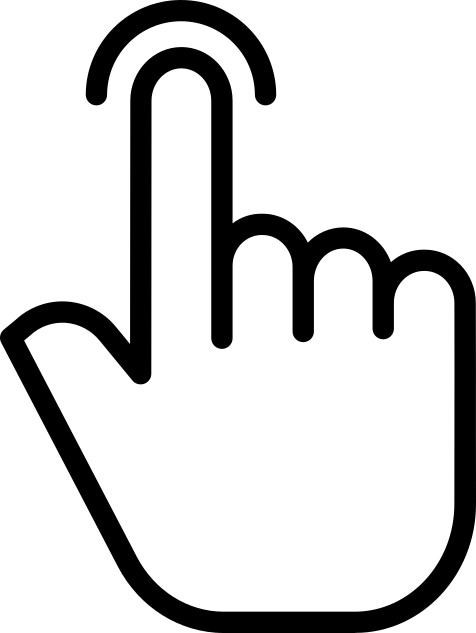
\includegraphics[width=0.10\textwidth]{static/dedo.png}} ;
    \node[const, left=of d] (nd) {\Large $S$};

    \edge {r} {d};
  }
  \caption{Modelo A}
  \label{fig:modelo_causal_1}
  \end{subfigure}
  \begin{subfigure}[b]{0.33\textwidth}
  \centering
  \tikz{

    \node[latent] (d) {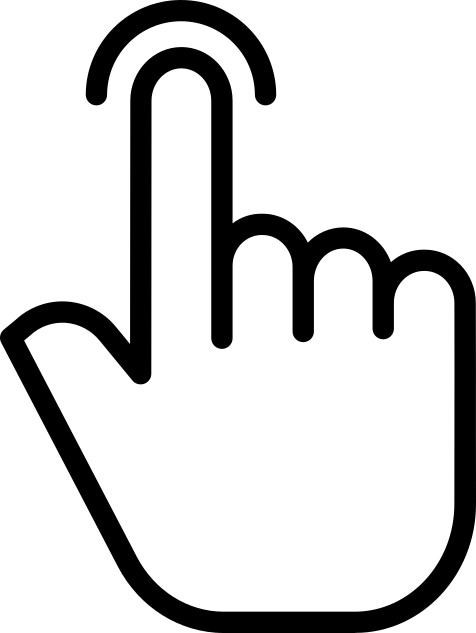
\includegraphics[width=0.10\textwidth]{static/dedo.png}} ;
    \node[const,above=of d] (nd) {\Large $S$} ;

    \node[latent, above=of d, yshift=-0.3cm, xshift=-1.2cm] (r) {
\includegraphics[width=0.12\textwidth]{static/regalo.png}} ;
    \node[const,left=of r] (nr) {\Large $\ \ R$} ;

    \node[latent, fill=black!30, above=of d, yshift=-0.3cm, xshift=1.2cm] (c) {
\includegraphics[width=0.12\textwidth]{static/cerradura.png}} ;
    \node[const,right=of c] (nc) {\Large $C=c_1$} ;

    \edge {r,c} {d};
  }
  \caption{Modelo B}
  \label{fig:modelo_causal_2}
  \end{subfigure}
  \caption{Modelos alternativos especificados como redes bayesianas. Los nodos representan las hipótesis, la flecha representa relaciones de dependencia entre hipótesis, y los nodos pintados de gris representan hipótesis ya conocidas (datos).
  En el Modelo A~\subref{fig:modelo_causal_1} la pista s\'olo depende de la posici\'on del regalo, no puede mostrarse el interior de la caja que contiene el regalo $P(r_i, s_i|c_1,M_A)=0$. En el Modelo B~\subref{fig:modelo_causal_2} la pista depende de la posici\'on del regalo y la caja elegida previamente, no puede mostrarse el interior de la caja que contiene el regalo, ni la caja elegida $P(r_i, s_i|c_1,M_B)=0$, $P(r_i, s_1|c_1,M_B)=0$.
  }
  \label{fig:modelos_causales}
\end{figure}


% Parrafo

En la figura~\ref{fig:modelo_causal_2} se especifica el modelo $B$ de forma gr\'afica a través de una red bayesiana.
%
En la notación de redes bayesianas, las hipótesis que finalmente son observadas (los datos) se agregan como nodos pintados de gris.
%
Es el caso de la hipótesis $C=c_1$, que aparece en la representación gráfica del modelo $B$.
%
En el modelo $A$ podríamos haber agregado el nodo, pero decidimos no hacerlo debido que según el modelo $A$ la hipótesis $C$ no interactúa con el resto de las hipótesis.

% Parrafo

Para calcular las distribuciones de probabilidad honesta, $P(R,S|c_1,M_A)$ y $P(R,S|c_1,M_B)$, analicemos en detalle las restricciones de los modelos.
%
En particular, cada modelo tiene asociado un conjunto de universos posibles.
%
En ambos modelos, el regalo puede estar indistintamente en cualquier caja.
%
Sin embargo, las cajas que se pueden mostrar dependen del modelo y la posición del regalo.
%
En el modelo $A$, si el regalo se encuentra en la caja 1, $R=r_1$, la caja que se nos muestra puede ser indistintamente $S=s_2$ o $S=s_3$.
%
De forma equivalente, para cada posible posición del regalo $R =r_i$, en el modelo $A$ nos pueden mostrar indistintamente cualquiera de las otras dos cajas.
%
En el modelo $B$, solo cuando la posición de regalo no coincide con la caja que elegimos, se nos puede mostrar indistintamente $s_2$ o $s_3$.
%
En el resto de los casos, cuando la elección de la caja no coincide con la posición del regalo, solo es posible que nos muestren una única caja.

% Parrafo

Aplicando el principio de indiferencia, la distribución honesta surge de dividir la probabilidad en partes iguales en cada una de las bifurcaciones de los universos paralelos que producen los modelos alterativos.
%
En la figura~\ref{fig:caminos} se representan el árbol de los posibles universos paralelos baja  cada uno de los modelos.
%
Cada camino que va de la raíz a una de las hojas representa un universo posible.
%
Los nodos de ese camino representan las hipótesis elementales que son ciertas en ese universo (o el estado del universo).
%
Y las bifurcaciones contienen una fracción que representa cómo se divide la probabilidad entre los universos paralelos (en este caso aplicando el principio de indiferencia en todos los niveles)

%

\begin{figure}[H]
\centering
\begin{subfigure}[b]{0.48\textwidth}
\centering
\tikz{
\node[latent, draw=white, yshift=0.7cm] (b0) {$\frac{1}{3}$};

\node[latent,below=of b0,yshift=0.7cm, xshift=-2cm] (r1) {$r_1$};
\node[latent,below=of b0,yshift=0.7cm] (r2) {$r_2$};
\node[latent,below=of b0,yshift=0.7cm, xshift=2cm] (r3) {$r_3$};

\node[latent, below=of r1, draw=white, yshift=0.7cm] (br1) {$\frac{1}{2}$};
\node[latent, below=of r2, draw=white, yshift=0.7cm] (br2) {$\frac{1}{2}$};
\node[latent, below=of r3, draw=white, yshift=0.7cm] (br3) {$\frac{1}{2}$};
\node[latent,below=of br1,yshift=0.7cm, xshift=-0.5cm] (r1d2) {$s_2$};
\node[latent,below=of br1,yshift=0.7cm, xshift=0.5cm] (r1d3) {$s_3$};

% \node[latent,below=of r1d2,yshift=0.7cm,draw=white] (br1d2) {$\frac{1}{3}\frac{1}{2}$};
% \node[latent,below=of r1d3,yshift=0.7cm, draw=white] (br1d3) {$\frac{1}{3}\frac{1}{2}$};
\node[latent,below=of br2,yshift=0.7cm, xshift=-0.5cm] (r2d1) {$s_1$};
\node[latent,below=of br2,yshift=0.7cm, xshift=0.5cm] (r2d3) {$s_3$};
\node[latent,below=of br3,yshift=0.7cm, xshift=-0.5cm] (r3d1) {$s_1$};
\node[latent,below=of br3,yshift=0.7cm, xshift=0.5cm] (r3d2) {$s_2$};

% \node[latent,below=of r2d1,yshift=0.7cm, draw=white] (br2d1) {$\frac{1}{3}\frac{1}{2}$};
% \node[latent,below=of r2d3,yshift=0.7cm,draw=white] (br2d3) {$\frac{1}{3}\frac{1}{2}$};
% \node[latent,below=of r3d1,yshift=0.7cm, draw=white] (br3d1) {$\frac{1}{3}\frac{1}{2}$};
% \node[latent,below=of r3d2,yshift=0.7cm,draw=white] (br3d2) {$\frac{1}{3}\frac{1}{2}$};
\edge[-] {b0} {r1,r2,r3};
\edge[-] {r1} {br1};
\edge[-] {r2} {br2};
\edge[-] {r3} {br3};
\edge[-] {br1} {r1d2,r1d3};
% \edge[-] {r1d2} {br1d2};
% \edge[-] {r1d3} {br1d3};
\edge[-] {br2} {r2d1, r2d3};
\edge[-] {br3} {r3d1,r3d2};
% \edge[-] {r2d1} {br2d1};
% \edge[-] {r2d3} {br2d3};
% \edge[-] {r3d1} {br3d1};
% \edge[-] {r3d2} {br3d2};
}
\caption{Modelo A}
\label{fig:caminos_pre_montyhall}
\end{subfigure}
\begin{subfigure}[b]{0.48\textwidth}
\centering
\tikz{
\node[latent, draw=white, yshift=0.7cm] (b0) {$\frac{1}{3}$};
\node[latent,below=of b0,yshift=0.7cm, xshift=-2cm] (r1) {$r_1$};
\node[latent,below=of b0,yshift=0.7cm] (r2) {$r_2$};
\node[latent,below=of b0,yshift=0.7cm, xshift=2cm] (r3) {$r_3$};

% \node[latent, below=of r1, draw=white, yshift=0.8cm] (br1) {$\frac{1}{3}$};
% \node[latent, below=of r2, draw=white, yshift=0.8cm] (br2) {$\frac{1}{3}$};
% \node[latent, below=of r3, draw=white, yshift=0.8cm] (br3) {$\frac{1}{3}$};
% \node[latent,below=of br1,yshift=0.8cm] (c11) {$c_1$};
% \node[latent,below=of br2,yshift=0.8cm] (c12) {$c_1$};
% \node[latent,below=of br3,yshift=0.8cm] (c13) {$c_1$};

\node[latent, below=of r1, draw=white, yshift=0.7cm] (bc11) {$\frac{1}{2}$};
\node[latent, below=of r2, draw=white, yshift=0.7cm] (bc12) {$1$};
\node[latent, below=of r3, draw=white, yshift=0.7cm] (bc13) {$1$};
\node[latent,below=of bc11,yshift=0.7cm, xshift=-0.5cm] (r1d2) {$s_2$};
\node[latent,below=of bc11,yshift=0.7cm, xshift=0.5cm] (r1d3) {$s_3$};
\node[latent,below=of bc12,yshift=0.7cm] (r2d3) {$s_3$};
\node[latent,below=of bc13,yshift=0.7cm] (r3d2) {$s_2$};

% \node[latent,below=of r1d2,yshift=0.7cm,draw=white] (br1d2) {$\frac{1}{3}\frac{1}{2}$};
% \node[latent,below=of r1d3,yshift=0.7cm, draw=white] (br1d3) {$\frac{1}{3}\frac{1}{2}$};
% \node[latent,below=of r2d3,yshift=0.7cm,draw=white] (br2d3) {$\frac{1}{3}$};
% \node[latent,below=of r3d2,yshift=0.7cm,draw=white] (br3d2) {$\frac{1}{3}$};
\edge[-] {b0} {r1,r2,r3};
% \edge[-] {r1} {br1};
% \edge[-] {r2} {br2};
% \edge[-] {r3} {br3};
% \edge[-] {br1} {c11};
% \edge[-] {br2} {c12};
% \edge[-] {br3} {c13};
\edge[-] {r1} {bc11};
\edge[-] {r2} {bc12};
\edge[-] {r3} {bc13};
\edge[-] {bc11} {r1d2,r1d3};
\edge[-] {bc12} {r2d3};
\edge[-] {bc13} {r3d2};
% \edge[-] {r1d2} {br1d2};
% \edge[-] {r1d3} {br1d3};
% \edge[-] {r2d3} {br2d3};
% \edge[-] {r3d2} {br3d2};
}
\caption{Modelo B}
\label{fig:caminos_montyhall}
\end{subfigure}
\caption{Los posibles universos dadas las restricciones de los modelos alternativos. Por el principio de indiferencia dividimos la creencia en partes iguales en cada una de las bifurcaciones de los caminos paralelos del modelo causal. Por simplicidad suponemos que $c_1$.}
\label{fig:caminos}
\end{figure}

% Parrafo

Luego, para calcular la probabilidad conjunta de que el regalo se encuentre en la caja $i$ y se nos muestre la caja $j$, $P(r_i, s_j|c_1,M)$, debemos multiplicar todas las fracciones presentes en cada uno de los caminos que van de la raíz a las hojas.
%
Los caminos no presentes en el árbol de universos paralelos se les debe asignar probabilidad 0 debido a que son caminos imposibles dadas las restricciones del modelo.
%
Esta informaci\'on la podemos resumir en forma de tabla~\ref{tab:creencia_conjunta}, que representa la probabilidad asignada a cada uno de los universos paralelos.
%
\begin{table}[ht!]
\centering
$P(r_i, s_j |c_1, M_A)$ \hspace{3cm} $P(r_i, s_j | c_1, M_B)$ \\[0.1cm]
 \begin{tabular}{|c|c|c|c|} \hline \setlength\tabcolsep{0.4cm}
       & \, $r_1$ \, &  \, $r_2$ \, & \, $r_3$ \, \\ \hline
  $s_1$ & $0$ & $1/6$ & $1/6$  \\ \hline
  $s_2$ & $1/6$ & $0$ & $1/6$  \\ \hline
  $s_3$ & $1/6$ & $1/6$ & $0$ \\ \hline
  \end{tabular}
  \hspace{1.5cm}
  \begin{tabular}{|c|c|c|c|} \hline  \setlength\tabcolsep{0.4cm}
 & \, $r_1$ \, &  \, $r_2$ \, & \, $r_3$ \,  \\ \hline
  $s_1$ & $0$ & $0$ & $0$ \\ \hline
  $s_2$ & $1/6$ & $0$ & $1/3$ \\ \hline
  $s_3$ & $1/6$ & $1/3$ & $0$  \\ \hline
  \end{tabular}
  \caption{Distribución de probabilidad honesta para cada uno de los modelos. Las celdas representan universos paralelos y el valor la probabilidad asignada a cada una de ellos.}
  \label{tab:creencia_conjunta}
\end{table}

% Parrafo

Una vez calculada la distribución de probabilidad conjunta honesta, podemos responder cualquier pregunta relacionada al problema de investigación mediante la aplicación estricta de las reglas de la probabilidad.
%
La regla de la suma establece que cualquier creencia marginal honesta puede ser obtenida integrando la creencia conjunta.
%
Por ejemplo, para obtener la probabilidad de la hipótesis $s_j$ debemos recuperar las probabilidades que asignamos a todos los universos paralelos en los que esa hipótesis elemental está presente,
%
\begin{equation} \label{eq:creencia_marginal}
\begin{split}
P(s_j|c_1,M_A) = \sum_{r_i \in R} P(r_i, s_j|c_1, M_A) = 1/3 \\
P(s_j|c_1,M_B) = \sum_{r_i \in R} P(r_i, s_j|c_1, M_B) = 1/2
\end{split}
\end{equation}
%
Esto es equivalente a sumar todos los elementos de una de las filas de la tabla.
%
Del mismo modo podemos calcular la probabilidad marginal de la hipótesis $R=r_i$.
%
En ese caso deberíamos sumar todos los elementos de una columna.
%
En ambos modelos, la probabilidad marginal sobre la posición del regalo es $1/3$.

% Parrafo

\begin{figure}[H]
\centering
\begin{subfigure}[b]{0.48\textwidth}
\centering
\tikz{ %
         \node[factor, minimum size=1cm] (p1) {
\includegraphics[width=0.05\textwidth]{static/cerradura.png}} ;
         \node[factor, minimum size=1cm, xshift=1.5cm] (p2) {} ;
         \node[factor, minimum size=1cm, xshift=3cm] (p3) {} ;

         \node[const, above=of p1, yshift=.15cm] (fp1) {$1/3$};
         \node[const, above=of p2, yshift=.15cm] (fp2) {$1/3$};
         \node[const, above=of p3, yshift=.15cm] (fp3) {$1/3$};
         \node[const, below=of p2, yshift=-.10cm, xshift=0.3cm] (dedo) {};
        }
\caption{$P(r_i|c_1,M)$}
\label{fig:prior_regalo}
\end{subfigure}
\begin{subfigure}[b]{0.48\textwidth}
\centering
\tikz{ %

         \node[factor, minimum size=1cm] (p1) {
\includegraphics[width=0.05\textwidth]{static/cerradura.png}} ;
         \node[det, minimum size=1cm, xshift=1.5cm] (p2) {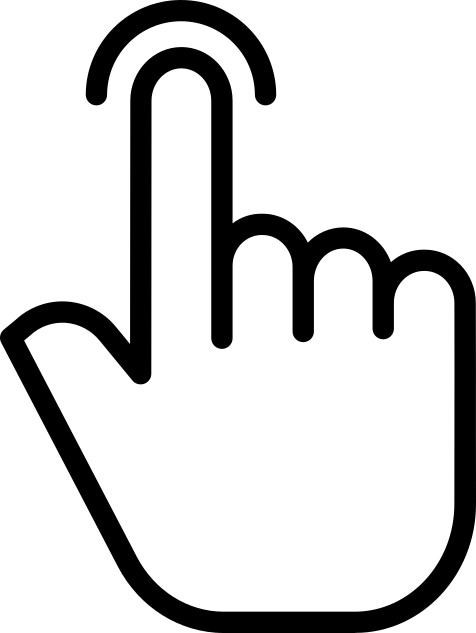
\includegraphics[width=0.06\textwidth]{static/dedo.png}} ;
         \node[factor, minimum size=1cm, xshift=3cm] (p3) {} ;
         \node[const, above=of p1, yshift=.15cm] (fp1) {$?$};
         \node[const, above=of p2, yshift=.15cm] (fp2) {$?$};
         \node[const, above=of p3, yshift=.15cm] (fp3) {$?$};
         \node[const, below=of p2, yshift=-.10cm, xshift=0.3cm] (dedo) {};

        }
\caption{$P(r_i|s_2,c_1,M)$}
\label{fig:posterior_regalo}
\end{subfigure}
\caption{En la figura~\ref{fig:prior_regalo} mostramos la distribución de probabilidad marginal de la hipótesis $R$ a priori. La cerradura representa la restricción $c_1$. En ambos modelos el prior sobre el regalo es el mismo. En la figura \ref{fig:posterior_regalo} nos preguntamos cuál es la distribución de probabilidad honesta sobre la posición del regalo luego de observar que la caja 2 está vacía.}
\end{figure}

% Parrafo

Para calcular la distribución de probabilidad honesta luego de observar que la caja dos está vacía, debemos aplicar la regla del producto.
%
La regla del producto simplemente codifica el principio de coherencia pues para calcularla nos debemos quedar únicamente con la creencia previa que siguen siendo compatibles con el observable, $P(r_i, s_2)$, esto es la fila de la distribución de probabilidad conjunta a priori correspondiente a la hipótesis elemental $s_2$.
%
\begin{table}[ht!]
\centering
$P(r_i, s_2 |c_1, M_A)$ \hspace{4.3cm} $P(r_i, s_2 | c_1, M_B)$ \\[0.1cm]
\begin{tabular}{|c|c|c|c||c|} \hline \setlength\tabcolsep{0.2cm}
       & \, $r_1$ \, &  \, $r_2$ \, & \, $r_3$ \, & \\ \hline
  $s_2$ & $1/6$ & $0$ & $1/6$ & $1/3$ \\ \hline
  \end{tabular}
  \hspace{1.5cm}
  \begin{tabular}{|c|c|c|c||c|} \hline  \setlength\tabcolsep{0.2cm}
 & \, $r_1$ \, &  \, $r_2$ \, & \, $r_3$ \, & \\ \hline
  $s_2$ & $1/6$ & $0$ & $1/3$ & $1/2$ \\ \hline
  \end{tabular}
  \caption{La creencia conjunta y marginal que sobrevive luego de ver el dato.}
  \label{tab:creencia_compatible}
\end{table}

% Parrafo

La probabilidad que sobrevive, $P(r_i, s_2|c_1,M)$, no representa todav\'ia nuestra nueva creencia total pues no integrar 1, $\sum_i P(r_i,s_2|c_1,M) = P(s_2|c_1,M) < 1$.
%
Para que la probabilidad que sobrevive sea considerada nuestra nueva creencia total necesitamos normalizarla para que en conjunto vuelva a sumar 1.
%
\begin{equation*}
\underbrace{P(r_i| s_2, c_1, \text{Modelo})}_{\hfrac{\text{Nueva creencia}}{\text{}}} = \frac{\overbrace{P(r_i, s_2|c_1, \text{Modelo})}^{\hfrac{\text{Creencia que}}{\text{sobrevive}}}}{\underbrace{P(s_2| c_1, \text{Modelo})}_{\hfrac{\text{Creencia total}}{\text{que sobrevive}}}}
\end{equation*}
%
Si multiplicamos a ambos lados por el denominador, obtenemos la expresi\'on de la regla del producto de la teor\'ia de la probabilidad.
%
La nueva distribuci\'on de probabilidad a la que llegamos depende del modelo elegido.
%
\begin{figure}[ht!]
\centering
\begin{subfigure}[b]{0.48\textwidth}
\centering
\tikz{ %

         \node[factor, minimum size=1cm] (p1) {
\includegraphics[width=0.05\textwidth]{static/cerradura.png}} ;
         \node[det, minimum size=1cm, xshift=1.5cm] (p2) {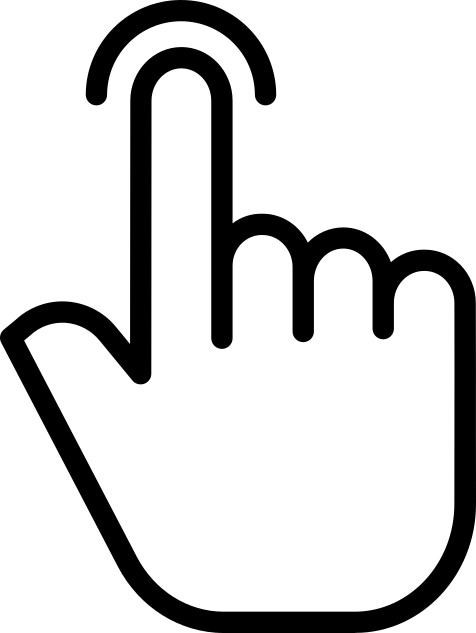
\includegraphics[width=0.06\textwidth]{static/dedo.png}} ;
         \node[factor, minimum size=1cm, xshift=3cm] (p3) {} ;

         \node[const, above=of p1, yshift=.15cm] (fp1) {$1/2$};
         \node[const, above=of p2, yshift=.15cm] (fp2) {$0$};
         \node[const, above=of p3, yshift=.15cm] (fp3) {$1/2$};
         \node[const, below=of p2, yshift=-.10cm, xshift=0.3cm] (dedo) {};
}
\caption{$P(r_i|s_2,c_1,M_A)$}
\end{subfigure}
\begin{subfigure}[b]{0.48\textwidth}
\centering
\tikz{ %

         \node[factor, minimum size=1cm] (p1) {
\includegraphics[width=0.05\textwidth]{static/cerradura.png}} ;
         \node[det, minimum size=1cm, xshift=1.5cm] (p2) {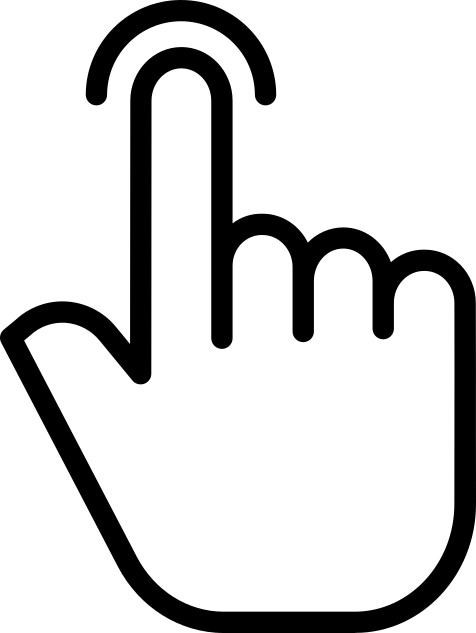
\includegraphics[width=0.06\textwidth]{static/dedo.png}} ;
         \node[factor, minimum size=1cm, xshift=3cm] (p3) {} ;

         \node[const, above=of p1, yshift=.15cm] (fp1) {$1/3$};
         \node[const, above=of p2, yshift=.15cm] (fp2) {$0$};
         \node[const, above=of p3, yshift=.15cm] (fp3) {$2/3$};
         \node[const, below=of p2, yshift=-.10cm, xshift=0.3cm] (dedo) {};
        }
\caption{$P(r_i|s_2,c_1,M_A)$}
\end{subfigure}
\caption{Distribución de probabilidad a posterior dado el dato $s_2$ y el modelo. El modelo $A$ asigna la misma probabilidad a la caja 1 y 3. El modelo $B$ asigna $1/3$ a la hipótesis $r_1$ y $2/3$ a la hipótesis $r_3$.}
\end{figure}
%
Si bien ambas respuesta son diferentes, ellas comparten la propiedad de ser la distribuci\'on de probabilidad honesta dada las restricciones.
%
Lo que hemos hecho no es otra cosa que aplicar el teorema de Bayes,
%
\begin{equation}
\begin{split}
\underbrace{P(r_i|s_2,c_1,M)}_{\text{Posterior}} = \frac{P(r_i,s_2|c_1,M)}{P(s_2|c_1,M)} = \frac{\overbrace{P(s_2|r_i,c_1,M)}^{\text{Verosimilitud}}\overbrace{P(r_i|c_1,M)}^{\text{Prior}}}{\underbrace{P(s_2|c_1,M)}_{\text{Evidencia}}}
\end{split}
\end{equation}

% Parrafo
% \subsubsection{Evidencia}
%
% De forma similar a la verosimilitud, la evidencia es una predicci\'on a priori del dato observado, pero que est\'a hecha con la contribuci\'on de todas las hip\'otesis.
% %
% Por la reglas de la probabilidad, el denominador del teorema de Bayes puede expresarse como una suma sobre todos los posibles valores del numerador, uno por cada hip\'otesis.
% %
% Esto hace que la evidencia sea constante para las diferentes hip\'otesis, por lo que puede ser ignorado cuando se comparan hip\'otesis alternativas.
% %
% Sin embargo, la evidencia va a ser distinta para los diferentes modelos.
% %
% En el modelo B la predicci\'on a priori de que la caja se\~nalada sea $s=2$, integrando todas las hip\'otesis, es $1/2$.
% %
% \begin{equation}
% P(s_2|M_B) = \sum_i P(s_2|r_i, M_B) P(r_i, M_B) = \frac{1}{2} \frac{1}{3} + 0 \frac{1}{3} + \frac{1}{1} \frac{1}{3} = 1/2
% \end{equation}
% %
% Mientras que en el modelo A la predicci\'on a priori de que la caja se\~nalada sea $s=2$, integrando todas las hip\'otesis, es $1/3$.
% %
% \begin{equation}
% P(s_2|M_A) = \sum_i P(s_2,r_i| M_A) = 1/3
% \end{equation}
% %
% Lo que ya hab\'ia sido calculado previamente en las marginales de la tabla \ref{eq:creencia_marginal}.
%
% % Parrafo
%
% La evidencia ser\'a de inter\'es cuando queramos evaluar modelos causales alternativos.
%
%
% \subsubsection{Evaluaci\'on de modelos alternativos}\label{sec:modelos_alternativos}

% Es una pr\'actica muy com\'un dejar impl\'icita la dependencia respecto del modelo causal.

% Parrafo

\subsection{Evaluación honesta de modelos}

Computar las distribuciones de probabilidad honesta dado los modelos no tendría ningún valor si la elección del modelo quedara librado al arbitrio de las subjetividades individuales.
%
¿Cuál de los dos modelos debemos usar?
%
¿Cuál de los dos posterior debemos reportar?
%
En la formulación del teorema de Bayes inicial~\eqref{eq:teorema_bayes} solo hay hipótesis y datos.
%
Sin embargo, los modelos tambi\'en son hip\'otesis, y por lo tanto, pueden ser evaluadas mediante la aplicación estricta de las reglas de la probabilidad.
%
Es decir, en el fondo nuestro problema de investigación (o experimento) $\mathcal{H}$ debe incluir también la hipótesis $M = \{M_A, M_B\}$, tal que $\mathcal{H} = \{R, S, M\}$.
%
Si aplicamos el teorema de Bayes para actualizar la probabilidad de los modelos $M$ dado los datos $D = \{r_i, s_j\}$ y la información incial $I = \{c_1\}$,
%
\begin{equation}\label{eq:p_modelo_|_datos}
 P(\text{Model\es{o}}|\text{Dat\en{a}\es{os}}, I) = \frac{\overbrace{P(\text{Dat\en{a}\es{os}}|\text{Model\es{o}}, I)}^{\text{Evidencia}}\overbrace{P(\text{Model\es{o}}|I)}^{\text{Prior}}}{P(\text{Dat\en{a}\es{os}}|I)}
\end{equation}
%
La evidencia es la predicción de los datos con la contribución de todas las hipótesis.
%
\begin{equation}
P(\text{Datos}|\text{Modelo},I) = \sum_{\text{Hipótesis}} P(\text{Datos}|\text{Hipótesis}, \text{Modelo},I) P(\text{Hipótesis}|\text{Modelo},I)
\end{equation}
%
Por la regla del producto, podemos expresar la evidencia conjunta de muchos datos $\{d_1, d_2, \dots \}$ como una productoria de predicciones a priori individuales,
%
\begin{equation} \label{eq:p<datos|modelo>}
\begin{split}
P(\text{Dat\en{a}\es{os}}=\{d_1, d_2, \dots \}|\text{Model\es{o}},I) & = P(d_1|\text{Model\es{o}},I)P(d_2|d_1,\text{Model\es{o}},I) \dots
\end{split}
\end{equation}
%
La probabilidad conjunta de todos los datos dado el modelo es igual a la probabilidad del primer dato $d_1$ dado el modelo, multiplicado por la probabilidad del segundo dato $d_2|d_1$ dado el primer dato y el modelo, y as\'i sucesivamente.
%
Notar que si alguna de las predicciones es $0$, toda la productoria se anula.
%
Por su parte, el denominador de la ecuaci\'on \ref{eq:p_modelo_|_datos} es la predicci\'on a priori del dato observado con la contribuci\'on de todos los modelos (y todas sus hip\'otesis).
%
\begin{equation}
P(\text{Datos}|I) = \sum_{\text{Modelo}} P(\text{Dat\en{a}\es{os}}|\text{Model\es{o}}, I) P(\text{Model\es{o}}, I)
\end{equation}

% Parrafo

Para evaluar los modelos generaremos datos sintéticos utilizando la distribución de la probabilidad del modelo $B$, $P(R,S|c_1,M_B)$, eligiendo primero la posici\'on del regalo $r_i$ a partir de la distribución $P(r_i|c_1,M_B)$ y eligiendo luego la pista $s_j$ a partir de la distribución $P(s_j|r_i,c_1,M_B)$.
%
Repetiremos el procedimiento $N$ veces, $t \in \{1, \dots, N\}$ .
%
Luego, nuestro problema de investigación (o experimento) contiene $\mathcal{H} = \{R_1, S_1, R_2, S_2, \dots, R_N, S_N, M_A, M_B\}$, con $R_t = \{r_{1t}, r_{2t}, r_{3t}\}$ y $S_t = \{s_{1t}, s_{2t}, s_{3t} \}$.
%
Vamos a considerar los mismos modelos, es decir, las mismas dependencias entre hipótesis al interior de cada repetición pero ninguna dependencia adicional entre repeticiones.
%
Las repeticiones se especifican en redes bayesianas mediante el uso de placas (ver figura~\ref{fig_modelos_con_repeticiones}).
%
\begin{figure}[ht!]
  \centering
  \begin{subfigure}[b]{0.33\textwidth}
  \centering
  \tikz{
    \node[latent,] (r) {
\includegraphics[width=0.12\textwidth]{static/regalo.png}} ;
    \node[const,left=of r] (nr) {\Large $R_t$} ;


    \node[latent, below=of r, yshift=0.3cm] (d) {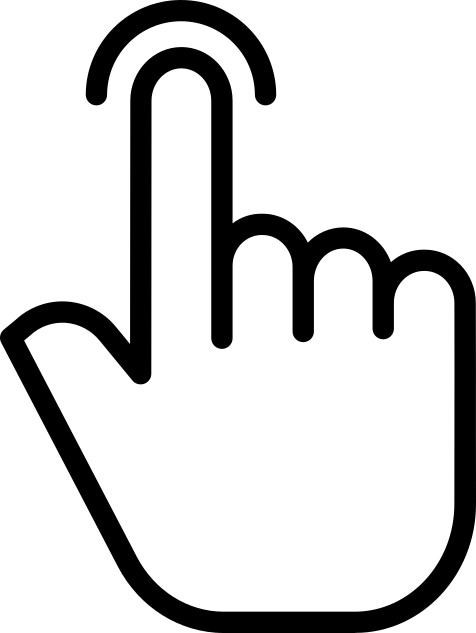
\includegraphics[width=0.10\textwidth]{static/dedo.png}} ;
    \node[const, left=of d] (nd) {\Large $S_t$};

    \edge {r} {d};
    \plate {Datos} {(r)(nr)(d)(nd)} {$t \in \{1, \dots N\} $}; %
  }
  \caption{Modelo A}
  \end{subfigure}
  \begin{subfigure}[b]{0.33\textwidth}
  \centering
  \tikz{

    \node[latent] (d) {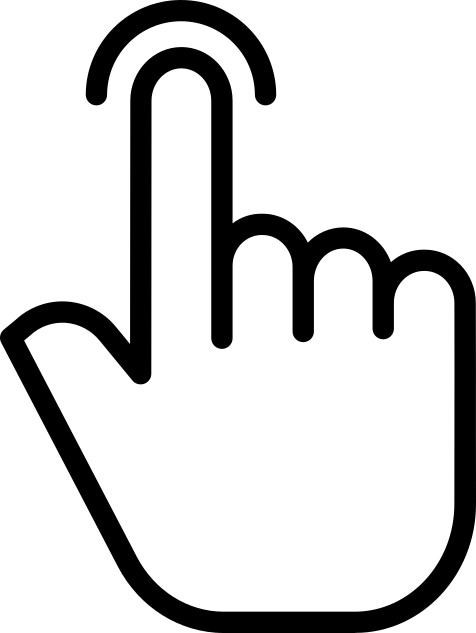
\includegraphics[width=0.10\textwidth]{static/dedo.png}} ;
    \node[const,above=of d] (nd) {\Large $S_t$} ;

    \node[latent, above=of d, yshift=-0.3cm, xshift=-1.2cm] (r) {
\includegraphics[width=0.12\textwidth]{static/regalo.png}} ;
    \node[const,left=of r] (nr) {\Large $\ \ R_t$} ;

    \node[latent, fill=black!30, above=of d, yshift=-0.3cm, xshift=1.2cm] (c) {
\includegraphics[width=0.12\textwidth]{static/cerradura.png}} ;
    \node[const,right=of c] (nc) {\Large $C_t=c_{1t}$} ;

    \edge {r,c} {d};
    \plate {Datos} {(r)(nr)(d)(nd)(c)(nc)} {$t \in \{1, \dots N\} $}; %
  }
  \caption{Modelo B}
  \end{subfigure}
  \caption{}
  \label{fig_modelos_con_repeticiones}
\end{figure}
%
Si se despliegan las placas de la figura~\ref{fig_modelos_con_repeticiones} veríamos N redes bayesianas, una al lado de la otra, sin dependencias que las vinculen entre sí.
%
El hecho de que no estén conectadas entre sí hace que los datos que se observan en una de las repeticiones no afecte al resto.
%
Luego, vamos a calcular la predicción de los datos dado los modelos $M = \{M_A, M_B\}$ y la información inicial $I = \{c_{11}, \dots, c_{1N}\}$,
%
\begin{equation}
P(\{r_{i1}, s_{j1}, \dots \}|M,I) = \prod_{t=1}^N P(s_{jt}|M,c_{1t})P(r_{it}|s_{jt},M,c_{1t})
\end{equation}
%
Debido a que los datos fueron generados usando la distribución de probabilidad el modelo $B$, los datos respetan las restricciones entre hipótesis presenten en el modelo $B$, y por lo tanto también la restricción entre hipótesis del modelo $A$.
%
Esto significa que no los modelos no observaran eventos imposibles.
%
Luego, las predicciones que hace el modelo $A$ son siempre las mismas debido que no importa cual sea la pista $s_{jt}$ y la posición del reaglo $r_{it}$, siempre vale $P(s_{jt}|M_A,c_{1t}) = 1/3$ y $P(r_{it}|s_{jt},M_A,c_{1t}) = 1/2$.
%
El modelo $B$ tambi\'en predice la pista siempre con la misma probabilidad $P(s_{jt}|M_A,c_{1t})=1/2$, pues no habr\'a en los datos generados $s_{1t}$.
%
Sin embargo, el modelo $B$ un tercio de las veces el regalo estará en la caja elegida, $P(r_{1t}|s_{jt},M_A,c_{1t}) = 1/3$, y dos tercios de las veces el regalo estará en la caja $i$ no elegida, $P(r_{it}|s_{jt},M_A,c_{1t}) = 2/3$, con $i\neq1$ y $i\neq j$.

\begin{equation}\label{eq:posterior_modelo_montyhall}
P(M_k|\overbrace{r_{i1},s_{j1}, \dots }^{\text{Datos}},\overbrace{c_1}^{I}) = \frac{\prod_{t=1}^N P(s_{jt}|M,c_{1t})P(r_{it}|s_{jt},M,c_{1t}) P(M_k|c_1)}{P(\text{Datos}|c_1)}
\end{equation}


R\'apidamente, con unas decenas de observaciones podemos tener una preferencia fuerte por modelo $B$, que es justamente el modelo que se utilizó para generar los datos.
%
\begin{figure}[H]
    \centering
    \begin{subfigure}[b]{0.45\textwidth}
    \includegraphics[width=\linewidth]{figures/monty_hall_selection.pdf}
    \end{subfigure}
    \caption{
    Selecci\'on de modelos alternativos
    }
    \label{fig:monty_hall_selection}
\end{figure}
%
Este mismo m\'etodo ser\'a usado para evaluar el modelo a lo largo de la tesis.


\subsection{Costo computacional y balance natural de las reglas de la probabilidad}

El obstáculo hist\'orico de la aplicaci\'on estricta de las reglas de la probabilidad ha sido el costo computacional asociado a la evaluaci\'on completa del las hip\'otesis de investigación (o experimento) $\mathcal{H} = \{H_1, H_2, \dots, H_N\}$.
%
En el caso más simple, con hip\'otesis de investigación binarias $|H_i|=2$, la cantidad de combinaciones (o universos paralelos) a evaluar, $P(h_1, h_2, \dots h_N)$, crece de forma exponencial $2^N-1$.
%
No solo hay que asignar probabilidades iniciales a cada una de esas combinaciones.
%
Hay que incorporar la información que transmite la observación de una hipótesis elemental en las restantes $2^N-2$ combinaciones a través del grado de sorpresa asociada a los supuestos iniciales del modelo o conjunto de restricciones
%(formalmente es la cantidad de probabilidad asignada por los supuestos a la hipótesis elemental que fue observada con anterioridad a que sea observada,predicción a priori).
%
En casos más complejos, que involucran además preguntas (o hipótesis) de investigación continuas ni siquiera es posible aplicar la regla de la suma cuando sus integrales no tiene solución analítica.
%
El famoso modelo lineal es un caso paradigmático en la historia de la probabilidad, es un modelo para el cual sus integrales tienen solución analítica pero que no pudo ser evaluado correctamente hasta el desarrollo de la computación moderna debido al costo computacional asociado a la inversión de matrices.

%

Revisemos el modelo lineal.
%
Comenzaremos a introducir lentamente algunos conceptos de causalidad.
%
Un modelo causal lineal de grado D supone que el mundo tiene $D+1$ causas ($W_0$ a $W_D$ con $D\geq 1$) que actúan sobre $N+1$ consecuencias ($Y_0$ a $Y_{N}$ con $N\geq1$) y que entre ellas existe la siguiente dependencias causales.
%
\begin{equation*} \label{eq:modelo_lineal}
y_i \leftarrow \sum_{d = 0}^{D} w_d x_d^d \hspace{1cm} \text{con $i \in \{0, \dots,N+1$}
\end{equation*}
%
La flecha representa la dependencia causal.
%
Esta notación, adoptada en el área de Inferencia Bayesiana Causal~\cite{pearl2009-causality}, involucra la idea de que cambios en los valores de las causas producen cambios en los valores de las consecuencias, pero no a la inversa.
%
Las hipótesis de investigación (o experimento) del modelo causal lineal más básico ($N=1, D=1$) son $\mathcal{H}=\{Y_0, Y_1, W_0, W_1\}$, con $Y_0=Y_1=W_0=W_1 = (-\infty, \infty)$.
%
\begin{equation*}
y_i \leftarrow  w_0 + w_1 x_i  \hspace{1cm}   \text{con $i \in \{0,1\}$}
\end{equation*}
%
Las variables $x_i \in (-\infty, \infty)$ no son hipótesis sino constantes que se nos informa con exactitud al recibir la observación de la hipótesis $Y_i$.
%
Las hipótesis $Y_1$ hasta $Y_N$ son observables.
%
A través de la observación de las consecuencias $Y_1$ a $Y_N$ tenemos que inferir el valor de las causas no observables $W_1$, $W_2$ y $W_3$ para predecir en todo el rango de $x_{N+1}$ el valor de la consecuencia todavía no observada $Y_{N+1}$.

% Parrafo

Al modelo lineal, se le agrega un elemento más.
%
Los valores observados $y_i$ se generan con un ruido aleatorio que tiene media 0 y desvío $\beta$.
%
La distribución honesta respecto a la información de la media y el desvío es la distribución Gaussiana o Normal.
%
\begin{equation}
P(y_i|x_i, w_1, w_2, w_3, \beta) = \N(y_i| w_0 + w_1 x_i + w_2 x_i^2,\ \beta^2)
\end{equation}
%
Esta es la distribución de probabilidad condicional de las hipótesis $Y_i$.
%
La distribución de probabilidad a priori de las causas $W_i$ son,
%
\begin{equation}
P(w_i|\sigma) = \N(w_i|0, \sigma )
\end{equation}
%
En la figura~\ref{fig:modelo_lineal} se especifica las dependencias entre hipótesis mediante una red bayesiana y las probabilidades condicionales de las hipótesis.
%
\begin{figure}[ht!]
    \centering
    \begin{subfigure}[c]{0.45\textwidth}
      \begin{equation*}
      \begin{split}
      p(y | x, \bm{w}, \beta ) &= \N(y \,|\, w_0 + w_1 x + w_2 x^2, \beta^2) \\[0cm]
      p(w_i) &= \N(w_i \,|\, 0, \sigma^2) \\[0cm]
      \end{split}
      \end{equation*}
    \end{subfigure}
    \begin{subfigure}[c]{0.45\textwidth}
    \centering
    \tikz{

    \node[latent, fill=black!100, minimum size=2pt] (beta) {} ; %
    \node[latent, fill=black!20, yshift=-1.5cm] (t) {$y_i$} ; %
    \node[latent, fill=black!100, yshift=-1.5cm , xshift=-2cm,minimum size=2pt] (x) {} ; %
    \node[const, above=of x] (c_x) {$x_i$};

    \node[const, above=of beta] (c_beta) {$\beta$};
    \node[latent, fill=black!0, yshift=-1.5cm, xshift=2cm] (w) {$w_d$};
    \node[latent, fill=black!100,yshift=-1.5cm, xshift=3.75cm, minimum size=2pt] (alpha) {} ; %
    \node[const, right=of alpha] (c_alpha) {$\sigma$};

    \node[latent, xshift=2cm] (ypred) {$y_{N+1}$} ; %
    \node[latent, fill=black!100, xshift=3.75cm, minimum size=2pt] (xpred) {} ; %
    \node[const, above=of xpred] (c_xpred) {$x_{N+1}$};


    \edge {x,beta,w} {t};
    \edge {beta,xpred,w} {ypred};
    \edge {alpha} {w};

    \node[invisible, above=of c_x, xshift=-0.2cm] (ia) {};
    \node[invisible, above=of w] (ib) {};


    \plate {no} {(x)(t)(ia)} {\scalebox{0.7}{$i \in \{1, \dots, N\}$}}; %
    \plate {si} {(w)(ib)} {\scalebox{0.7}{$d \in \{1, \dots, D\} $}}; %
    }
    \end{subfigure}
    \caption{Modelo causal lineal. Continuamos con la notación de redes bayesianas presentada en la figura~\ref{fig:modelos_causales}. Los puntos negros representan constantes.}
    \label{fig:modelo_lineal}
\end{figure}

% Parrafo

La distribución de probabilidad a posteriori sobre las causas, $P(\bm{w}|\bm{y}, \bm{x}, \sigma)$, y la predicción de la próxima consecuencia $P(y_{N+1}|x_{N+1}, \bm{w}, \bm{y}, \bm{x}, \beta)$, ambas son distribuciones Gaussianas conocidas (capítulo 2~\cite{Bishop2006}).
%
El vector $\bm{w}$ contiene las hipótesis elementales de $w_1$ a $w_D$, el vector $\bm{y}$ contiene las hipótesis elementales de $y_1$ a $y_N$, y el vector $\bm{x}$ contiene los valores $x_1$ a $x_N$.
%
Ante la dificultad para resolver la inferencia de este modelo aplicando estrictamente las reglas de la probabilidad, durante el siglo 20 se adoptó el hábito de seleccionar una \'unica hip\'otesis en base a alg\'un criterio ad-hoc, como por ejemplo \emph{maximo a posteriori}.
%
\begin{equation*}
 \underset{\bm{w}}{\text{ max }} P(\bm{y} | \bm{x}, \bm{w}, \beta) P(\bm{w}|\sigma)
\end{equation*}
%
donde la función $\bm{\phi}$ devuelve un vector de longitud $D$ con la transformación que sufre la variable $x_i$ en cada caso.
%
Y también se adoptó un procedimiento ad-hoc, que incluye una etapa llamada de ``entrenamiento'' y una etapa
%


Si bien este enfoque permiti\'o durante el siglo 20 ``ajustar'' funciones lineales a los datos, introdujo al mismo una serie de problemas que siguen presente en muchos de los algoritmos de inteligencia artificial modernos.

% Parrafo

Supongamos que tenemos un conjunto de datos generados a partir de una funci\'on objetivo que decidimos modelar con polinomios de distinto grado $n \in \{0, 1, \dots, 9\}$.
%
\begin{equation*}
y = \sum_{i=0}^n w_i \, x^i
\end{equation*}
%
Una inc\'ognita muy b\'asica que quisi\'eramos resolver en general es determinar cu\'al es el mejor modelo.
%
El problema de los enfoques que seleccionan una \'unica hip\'otesis es precisamente el uso de criterios ad-hoc.
%
Sin poder recurrir a las reglas de la probabilidad para evaluar modelos, ?`qu\'e significar\'ia que un modelo es mejor que otro?

% Parrafo

La funci\'on objetivo es una sinoidal $\N(y \,| \, \text{sen}(x), \beta^2)$ en el rango $x \in [-\pi,\pi]$ (l\'inea punteada en figura~\ref{fig:model_selection_OLS}).
%
En este caso, si bien ning\'un modelo es cierto, el modelo de grado 3 (l\'inea roja en figura~\ref{fig:model_selection_OLS}) deber\'ia ser suficiente para ajustar la funci\'on objetivo.
%
Sin embargo, al evaluando por m\'axima la versoimilutd nos encontramos con el hecho de que la verosimilutd crece indefinidamente a medida que le agregamos complejidad (grados) a los modelos.
%
El problema es que el modelo de grado 9 (l\'inea celeste en figura~\ref{fig:model_selection_OLS}), a pesar de ser el que m\'as cerca pasa por los todos puntos observados, no es el que m\'as cerca pasa por la funci\'on objetivo oculta, y por lo tanto no ser\'a el que mejor desempe\~no tenga sobre los datos nuevos.

% Parrafo

\begin{figure}[ht!] \centering
  \begin{subfigure}[t]{0.32\textwidth}
  \centering
  \includegraphics[width=0.9\textwidth]{figures/pdf/model_selection_OLS.pdf}
  \caption{Ajuste de modelos}
  \label{fig:model_selection_OLS}
  \end{subfigure}
  \begin{subfigure}[t]{0.32\textwidth}
  \centering
  \includegraphics[width=0.9\textwidth]{figures/pdf/model_selection_maxLikelihood.pdf}
  \caption{Verosimilitud de modelos}
  \label{fig:model_selection_maxLikelihood}
  \end{subfigure}
  \begin{subfigure}[t]{0.32\textwidth}
  \centering
  \includegraphics[width=0.9\textwidth]{figures/pdf/model_selection_maxApriori_online.pdf}
  \caption{Validaci\'on en l\'inea}
  \label{fig:model_selection_maxApriori_online}
  \end{subfigure}
  \caption{Modelos polinomiales de grado 0 a 9 ajustados por m\'axima versoimilutd a datos generados con una sinodal, $\N(y \,| \, \text{sen}(x), \beta^2) \ \ x \in [-\pi,\pi]$. Los modelo de grado 3 y 9 se muestran en rojo y celeste respectivamente.}
  \label{fig:overfitting}
\end{figure}

% Parrafo

Este problema se lo conoce con el nombre de \emph{overfitting} y en parte surge debido a que la predicci\'on de los modelos que estamos evaluando no ``pre-dice'' en sentido estricto, debido a que antes seleccionamos los par\'ametros que mejor ajustaban los datos.
%
\begin{align*}
\widehat{P}(\text{dato}|\text{Modelo}) & = P(\text{dato} \, | \, \overbrace{\underset{h}{\text{arg max}} \ P(\text{dato}|h, \text{Modelo})}^{\text{Hip\'otesis que mejor predice}},  \, \text{Modelo} )
\end{align*}
%
Ser\'ia m\'as honesto decir que el modelo ``post-dice'', dice despu\'es de haber visto los datos.
%
Para evitar esta ``trampa'', los enfoques que usan criterios ad-hoc para seleccionar hip\'otesis se ven obligados a evaluar modelos separando los datos en al menos dos partes: una para ``entrenar'', para seleccionar la hip\'otesis al interior del modelo; y otra para ``evaluar'', para seleccionar el modelo que mejor predice.
%
\begin{align*}
\widehat{P}(\text{dato}_{\textbf{Evaluar}}|\text{Modelo}) & = P(\text{dato}_{\textbf{Evaluar}} \, | \, \underset{h}{\text{arg max}} \ P(\text{dato}_{\textbf{Entrenar}}|h, \text{Modelo}),  \, \text{Modelo} )
\end{align*}
%
Si revisamos la definici\'on exacta que dan las reglas de la probabilidad de $P(\text{Datos}|\text{Modelo})$ (ecuaci\'on~\ref{eq:p<datos|modelo>}), observamos que se trata de una secuencia de predicciones del siguiente dato, con la informaci\'on de todos los datos anteriores.
%
Las reglas de la probabilidad nos resuelven este problema de forma  autom\'atica.
%
Si emulamos este procedimiento ``online'' que se observa en la descomposici\'on (\ref{eq:p<datos|modelo>}), entrenando el modelo en cada iteraci\'on y prediciendo el sieguiente dato, encontramos que el modelo que mejor predice es el modelo de grado 3 (figura~\ref{fig:model_selection_maxApriori_online}).

% Parrafo

Si bien parece que hemos resuelto el problema principal, sigue sobreajustando los datos.
%
Pues si comenzamos a observar puntos por fuera del rango $[-\pi, \pi]$, el modelo de grado 3 va a tener un p\'esimo desempe\~no.
%
Con los criterios ad-hoc aparce siempre, por alg\'un lado, el problema.

% % Parrafo
%
% Para explicar el comportamiento del modelo lineal basado en la aplicaci\'on estricta de las reglas de la probabilidad vamos a ver c\'omo se actualizan las distribcuiones de creencias a medida que vamos observando datos en un modelo que tiene solo dos par\'ametros, $y = w_0 + w_1 x$ (figura~\ref{fig:modelo_lineal_actualizaciones}).
% %
% Antes de observar el primer dato (ver la primera fila de la figura~\ref{fig:modelo_lineal_actualizaciones}) tenemos una distribuci\'on de creencias sobre los par\'ametros centrada en $0$ y con mucha incertidumbre (el eje $x$ e $y$ representa la ordenada al origen y la pendiente, y el punto rojo reprersenta el verdadero valor que queremos estimar).
% %
% Si usamos esa distribuci\'on a priori para muestrar valores del espacio de hip\'otesis, vamos a obtener combinaciones de ordenada al origen y pendiente que nos genera las rectas que se observan en la tercer columna.
%
% % Parrafo
%
%  \begin{figure}[ht!]
% \begin{subfigure}[t]{0.32\textwidth}
% \caption*{Verosimilitud}
% \end{subfigure}
% \begin{subfigure}[t]{0.32\textwidth}
% \caption*{Priori/Posteriori}
% \includegraphics[width=\textwidth]{figures/pdf/linearRegression_posterior_0.pdf}
% \end{subfigure}
% \begin{subfigure}[t]{0.32\textwidth}
% \caption*{Espacio de datos}
% \includegraphics[width=\textwidth]{figures/pdf/linearRegression_dataSpace_0.pdf}
% \end{subfigure}
%
%
% \begin{subfigure}[c]{0.32\textwidth}
% \includegraphics[width=\textwidth]{figures/pdf/linearRegression_likelihood_1.pdf}
% \end{subfigure}
% \begin{subfigure}[c]{0.32\textwidth}
% \includegraphics[width=\textwidth]{figures/pdf/linearRegression_posterior_1.pdf}
% \end{subfigure}
% \begin{subfigure}[c]{0.32\textwidth}
% \includegraphics[width=\textwidth]{figures/pdf/linearRegression_dataSpace_1.pdf}
% \end{subfigure}
%
% \begin{subfigure}[c]{0.32\textwidth}
% \includegraphics[width=\textwidth]{figures/pdf/linearRegression_likelihood_2.pdf}
% \end{subfigure}
% \begin{subfigure}[c]{0.32\textwidth}
% \includegraphics[width=\textwidth]{figures/pdf/linearRegression_posterior_2.pdf}
% \end{subfigure}
% \begin{subfigure}[c]{0.32\textwidth}
% \includegraphics[width=\textwidth]{figures/pdf/linearRegression_dataSpace_2.pdf}
% \end{subfigure}
% \caption{Actualizaci\'on de la distribuci\'on de creencias en un modelo lineal con ordenada al origen y pendiente. En las primeras dos columnas, los ejes $x$ e $y$ representan la ordenada al origen $w_0$ y la pendiente $w_1$ respectivamente. En la tercer columna los ejes $x$ e $y$ representan los datos $x$ e $y$ respectivamente.´}
% \label{fig:modelo_lineal_actualizaciones}
% \end{figure}
%
% % Parrafo
%
% La verosimilitud del primer dato (segunda fila de la figura~\ref{fig:modelo_lineal_actualizaciones}) asigna valores altos (regi\'on amarilla) a la combinaci\'on de ordenadas al origen y pendientes que pasan cerca del punto negro (en la tercera columna).
% %
% Al multiplicar la verosimilitud por el creencia previa, obtenemos el primer poterior (gr\'afico central).
% %
% Luego de observar un segundo dato (tercera fila) y repetir la operaci\'on, obtenemos un posterior muy cercano al verdadero valor.
%
% % Parrafo

%
% \subsection{El balance natural de las reglas de la probabilidad}
?`La aplicaci\'on estricta de las reglas de la probabilidad produce sobreajuste?
%
Los modelos polinomiales que estamos implementando tienen soluci\'on anal\'itica, por lo que hoy en d\'ia podemos pedirle a la computadora que calcule la predicci\'on exacta que hace cada uno de elos, $P(\text{Datos}|\text{Modelo})$, y calcular entonces el posterior exacto $P(\text{Modelo}|\text{Datos})$ .
%
Aplicando las reglas de la probabilidad obtenemos un resultado interesante.
%
\begin{figure}[ht!] \centering
  \begin{subfigure}[t]{0.32\textwidth}
  \centering
  \includegraphics[width=0.9\textwidth]{figures/pdf/model_selection_MAP_non-informative.pdf}
  \caption{Ajuste bayesiano}
  \label{fig:model_selection_MAP_non-informative}
  \end{subfigure}
  \begin{subfigure}[t]{0.32\textwidth}
  \centering
  \includegraphics[width=0.9\textwidth]{figures/pdf/model_selection_evidence.pdf}
  \caption{Posterior de modelos}
  \label{fig:model_selection_evidence}
  \end{subfigure}
  \caption{Modelos polinomiales de grado 0 a 9 ajustados mediante las reglas de la probabilidad a datos generados con una sinodal, $\N(y \,| \, \text{sen}(x), \beta^2) \ \ x \in [-\pi,\pi]$.}
  \label{fig:evaluacion_de_modelo}
\end{figure}

% Parrafo

La alicaci\'on estricta de las reglas de la probabilidad no produce ninguno de los sobreajustes que vimos en la secci\'on anterior quye emergen de los enfoques con criterios ad-hoc.
%
En primer lugar, el modelo que tiene la complejidad m\'inima necesaria (el de grado 3), es el que recibe mayor probabilidad a posteriori.
%
Al mismo tiempo, los modelos con complejidad mayor a la necesaria no son rechazados.
%
Todos ellos reciben una probabilidad visiblemente mayor a 0.
%
Si empezamos a ver datos por fuera del rango $[-\pi, \pi]$, estos modelos complejos iran a nuestro rescate, podr\'an explicar los nuevos datos.
%
Los \'unicos modelos rechazados son los que tienen menor complejidad de la necesaria (grado 0 a 2).

% Parrafo

Este balance surge naturalemente de las reglas de la probabilidad.
%
Por definici\'on, toda distribuci\'on de creencias debe sumar o integrar 1.
%
Los modelos que m\'as complejos, al ser m\'as flexibles, distribuyen la predicci\'on en un espacio m\'as amplio que los modelos m\'as simples.
%
Esto hace que siempre haya una regi\'on donde los modelos m\'as simples ganan, y otra donde los modelos m\'as complejos ganan.
%
Supongamos que recibimos un datos $x = 0.2$.
%
En la figura~\ref{fig:balance_natural} vemos la predicci\'on que hacen los distintos modelos de la variable $y$.
%
\begin{figure}[ht!] \centering
 \includegraphics[page=2,width=0.45\textwidth]{figures/pdf/evidencia_de_modelos_alternativos}
  \caption{Representa la predicci\'on que los diversos tipos de modelos polinomiales (clasificados por su complejidad) hacen de la variable $y$ para $x=0.2$.}
  \label{fig:balance_natural}
\end{figure}

% Parrafo

Los modelos r\'igidos (grado 0 a 2) colocan toda su creencia en una regi\'on lejana al verdadero valor, por lo que siempre tienen un mal desempe\~no predictivo.
%
Los modelos simples (grado 3), la mayor parte de su creencia sobre el verdadero valor.
%
Y los modelos complejos (grado 4 a 9) tambi\'en ponen la mayor parte de su creencia sobre el verdadero valor, pero distribuyen tambi\'en algo de creencia hacia los costados.
%
Dependiendo de d\'onde caiga el siguiente dato, hay una regi\'on en la que gana el modelo m\'as simple, y hay otra regi\'on donde gana el modelo m\'as complejo.

% Parrafo

A diferencia de los enfoque basados en criterios ad-hoc, la aplicaci\'on estricta de las reglas de la probabilidad realiza las predicciones con la contribuci\'on de todas las hip\'otesis.
%
Por la regla de la suma, podemos expresar la evidencia como una suma de las predicciones conjuntas realizadas individualmente por cada una de sus hip\'otesis.
%
\begin{equation}
\begin{split}
P(\text{Dat\en{a}\es{os}}|\text{Model\es{o}}) & = \sum^{\text{Hip\'otesis}}_h P(\text{Dat\en{a}\es{os}}|h,\text{Model\es{o}}) P(h|\text{Model\es{o}})
\end{split}
\end{equation}
%
Con que una \'unica hip\'otesis asigne a los datos probabilidad mayor a $0$, la evidencia tambi\'en ser\'a mayor a $0$, evitando as\'i el peor caso.
%
De esta forma, las hip\'otesis de un mismo modelo cooperan en la predicci\'on a priori de los datos observados, evitando los problemas de sobreajuste asociados a los enfoque que seleccionan una \'unica hip\'otesis del espacio.
%
Combinando la regla del producto y de la suma podemos expresar la evidencia como una productoria de sumatorias.
%
 \begin{equation}
\begin{split}
P(\text{Dat\en{a}\es{os}}|\text{Model\es{o}}) & = P(d_1|\text{Model\es{o}})P(d_2|d_1,\text{Model\es{o}}) \dots \\
& = \left( \sum^{\text{Hipo}}_h P(d_1|h,\text{M}) P(h|\text{M}) \right) \left( \sum^{\text{Hipo}}_h P(d_2|d_1,h,\text{M}) P(h|d_1,\text{M}) \right)  \dots \\\end{split}
\end{equation}
%
Cada predicci\'on individual de la productoria es una en el fondo una media aritm\'etica.
%
As\'i, el modelo reduce fluctuaciones en cada una de las predicciones individuales a trav\'es de la contribuci\'on que realiza el conjunto de sus hip\'otesis.




\section{Cuestiones relativas a la operacionalizaci\'on del los datos} \label{sec:base_empirica_metodo}



El problema fundamental de la teor\'ia de la informaci\'on es el de la comunicaci\'on con la realidad.
%
En palabras de Claude Shannon~\cite{shannon1948-theoryOfCommunication},
%
\begin{quotation}
The fundamental problem of communication is that of reproducing at one point either exactly or approximately a message selected at another point.
(\dots).
The significant aspect is that the actual message is one selected from a set of possible messages.
The system must be designed to operate for each each possible selection, not just the one which will actually be chosen since this is unknown at the time of design.
\end{quotation}
%
En ciencias empíricas, al no tener acceso directo a la realidad, debemos inferirla a partir de los mensajes distorsionados e indirectos que percibimos.
%

%
Quisi\'eramos que el mensaje que recibimos de la realidad sea igual al enviado.
%
Las soluciones a este problema se suelen dividir en dos tipos~\cite{Mackay2003}.
%
Una soluci\'on f\'isica, que podr\'ia ser ``acercarse para escuchar mejor''.
%
Y una soluci\'on inferencial, que ser\'ia simplemente interpretar la se\~nal con ruido que recibimos.
%
En cualquier caso, la soluci\'on f\'isica tambi\'en requiere resolver un proceso de inferencia.
%
En definitiva, el problema consiste en que nunca tenemos contacto directo con la realidad.
%
Ni siquiera nuestras propias percepciones son la realidad externa, sino el resultado de una maquinaria biol\'ogica sumamente compleja.
%
En este contexto ?`c\'omo podemos hacer para acceder a la realidad?
%
?`Cu\'al es el conjunto de elementos del mundo que sirven de evidencia indubitable (dato)?

\subsection{Base emp\'irica y datos T-te\'oricos}

Llamamos \emph{base emp\'irica} a la porci\'on del ``mundo'' que es aceptada como verdad por una comunidad, al menos por un cierto momento.
%
Para aceptar la entidad de nuestros objetos m\'as cotidianos, como por ejemplo el precio al que ayer nos vendieron los tomates en la verduler\'ia, o el resultado de la final de los \'ultimos mundiales de f\'utbol, son suficientes los supuestos del sentido com\'un.
%
A pesar de que existan c\'irculos filos\'oficos que pretendan poner en duda las percepciones y supuestos m\'as b\'asicos, reduciendo la base emp\'irica a un conjunto vac\'io (que Klimovsky~\cite{klimovsky1994-desventuras} llama \emph{base emp\'irica filos\'ofica}), en la vida cotidiana no hay mayor controversia al respecto.
%
Los objetos que cualquier persona tomar\'ia por ciertos en su vida cotidiana constituyen una base emp\'irica significativamente m\'as amplia, que llama \emph{base emp\'irica epistemol\'ogica}, pues son la base de control inicial de toda actividad cient\'ifica.
%
Sin embargo, a medida que la ciencia y la t\'ecnica avanza, el resultado de algunos nuevos instrumentos de medici\'on, como la temperatura atmosf\'erica o la inflaci\'on, pasan a ser aceptados como ``datos'' indubitable cuando las hip\'otesis o teor\'ias sobre los que est\'an construidos dejan de estar en duda al interior de cierta comunidad.
%
El conjunto de objetos que incluye aquellos objetos derivados de los nuevos acuerdos cient\'ificos se lo conoce como \emph{base emp\'irica metodol\'ogica}~\cite{klimovsky1994-desventuras}.

% Parrafo

Visto de esta forma, la definici\'on de base emp\'irica depende del conjunto de supuestos que una comunidad est\'a dispuesta a admitir sin poner en duda.
%
Los diferentes niveles de supuestos producen diferentes niveles de bases emp\'iricas, que formar\'ian una estructura en ``capas de cebolla'', con un n\'ucleo de base emp\'irica epistemol\'ogica y capas sucesivas $i$ de bases emp\'iricas metodol\'ogicas, BEM$_i$.
%
Para que uno de los niveles pueda actuar como base emp\'irica de control de una teor\'ia de nivel superior, es necesario que sus supuestos queden fuera de toda duda al momento de realizar la evaluaci\'on.
\begin{figure}[ht!]
    \centering
    \begin{subfigure}[b]{0.48\textwidth}
    \includegraphics[page=4,width=\linewidth]{figures/baseEmpirica.pdf}
    \end{subfigure}
    \caption{Niveles de base emp\'irica. En negro la base emp\'irica epistemol\'ogica, en gris las bases emp\'iricas metodol\'ogicas, y en blanco los instrumentos de medici\'on o inferencia que todav\'ia no han alcanzado un acuerdo intersubjetivo amplio, que dependen de la aceptaci\'on de una nueva teor\'ia T.}
\end{figure}

% Parrafo

Si los datos son una construcci\'on te\'orica entonces, concluyen los cr\'iticos, se pierde todo control externo y la ciencia no ser\'ia m\'as que un juego de auto justificaci\'on.
%
Sin embargo, es el concepto mismo de base emp\'irica como construcci\'on relativa a supuestos lo que permite superar esa cr\'itica pertinente.
%
La actividad cient\'ifica mantiene su control externo en tanto existe siempre un conjunto de datos que si bien est\'an cargados de supuestos, no lo est\'an de los supuestos de la teor\'ia para los que son datos.
%
En palabras de D\'iez y Lorenzano~\cite{lorenzano2002-concepcionEstructuralista},
%
\begin{quotation}
Un t\'ermino, un concepto, o una entidad, no es te\'orico o no te\'orico sin m\'as, sino relativamente a una teor\'ia dada.
Por eso no se debe hablar tanto de teoricidad cuanto de T-teoricidad, teoricidad relativa a la teor\'ia T. (...).
La idea es que un concepto es T-te\'orico si no se puede determinar sin presuponer la aplicabilidad de T, si todo procedimiento para su determinaci\'on la presupone; y puede obtenerse sin presuponer tal teor\'ia, si tiene alg\'un procedimiento de determinaci\'on T-independiente, por m\'as que tambi\'en tenga otros T-dependientes.
\end{quotation}
%
Los datos T-no te\'oricos son la base emp\'irica de control para una teor\'ia T pues pueden ser construidos mediante teor\'ias independientes, previamente aceptadas.

% En la secci\'on ``\nameref{sec:modelos_alternativos}'' hemos visto c\'omo garantizar los acuerdos intersubjetivos en la evaluaci\'on de los modelos causales alternativos.
% %
% En el cap\'itulo \ref{ch:ttt} seleccionamos el modelo de estimaci\'on de habilidad estado-del-arte en la industria del video juego, conocido como TrueSkill Through Time (TTT).



\subsection{La estructura invariante del dato emp\'irico} \label{sec:estructura_invariante}

Los datos cient\'ificos son funciones proposicionales, $f(x)=y$, donde la $x$ representa la unidad de an\'alisis, $f$ la variable, y la $y$ el valor de la variable.
%
%La estructura funcional de las proposiciones emp\'iricas obliga que se cumpla la propiedad de replicabilidad: cada vez que se vuelve a medir la misma variable sobre la misma unidad de an\'alisis debemos obtener el mismo resultado.
%
Al conversar informalmente usamos estas estructuras funcionales para expresar, por ejemplo, que la habilidad de Maradona fue superior a la de Messi, o que la ideolog\'ia del partido comunista es comunista.
%
\begin{align*}\label{eq:opiniones}
& \emph{Habilidad}(\text{Maradona}) > \emph{Habilidad}(\text{Messi}) \\[0.0cm]
& \textit{Ideolog\'ia}(\text{Partido Comunista}) = \text{Comunista}
\end{align*}
%
Las funciones \emph{Habilidad} e \emph{Ideolog\'ia} representan variables o caracter\'isticas que aplicadas sobre una unidad de an\'alisis particular, un jugador de f\'utbol o un partido pol\'itico, tienen un valor determinado, a pesar de que a veces no lo conozcamos con certidumbre.

% Parrafo

La estructura funcional, $f(x)=y$, es tan solo la parte abstracta del dato emp\'irico, su parte formal.
%
Esto es lo que permite usar modelos matem\'aticos o simulaciones computacionales, artefactos puramente formales, para describir sistemas naturales puramente emp\'iricos.
%
Cuando conversamos, constantemente nos expresamos usando funciones proposicionales de este tipo.
%
Sin embargo, raramente hacemos expl\'icita la definici\'on precisa de la funci\'on, por lo que dos personas pueden usar la misma palabra para expresar conceptos que en el fondo son distintos.
%
Ah\'i radica el origen de muchos de los desacuerdos que se producen en ciencia y en la vida cotidiana pues el significado preciso del dato depende de su ``operacionalizaci\'on'', del procedimiento preciso que una vez aplicado sobre una unidad de an\'alisis nos devuelve el valor de la variable.
%
Estos elementos de la praxis, que son los que determinan en los hechos el valor concreto que adquieren los conceptos abstractos, forman tambi\'en parte de la estructura de todo dato emp\'irico.

% Parrafo

%Debemos esta propuesta al epistem\'ologo Argentino, contempor\'aneo de Gregorio Klimovsky y Rolando Garc\'ia, el profesor Juan Samaja.

El epistem\'ologo Juan Samaja~\cite{Samaja1999} propone una hip\'otesis falsable (que \'el desaf\'ia a que encuentren un contra-ejemplo), de que todo dato emp\'irico se compone de dimensiones (D), que son especificaciones de la variable (V), y de procedimientos o protocolos (P), acciones que efectuadas sobre cierta fuente de datos (F) producen se\~nales o indicadores (I), objetos perceptibles desde el sentido com\'un, que interpretados con alguna hip\'otesis indicadora definen los resultados (R).
%
Samaja representa la estructura invariante del dato emp\'irico mediante el siguiente esquema (cuadro~\ref{tab:matriz_datos}).
%
\begin{table}[ht!]
\centering \footnotesize
\begin{tabular}{cccc}
$f$ & \normalsize $x$ &\normalsize  = & $y$    \\
  \normalsize  Variable (V) & \normalsize  Unidad de An\'alisis (UA) &\normalsize   &\normalsize  Resultado (R)    \\ \hline
 $\downarrow$ &$\downarrow$&&$\uparrow$ \\
 Examen de representatividad &Examen de viabilidad & & Hip\'otesis indicadora \\
 $\downarrow$ &$\downarrow$&&$\uparrow$ \\
 \normalsize Dimensiones (D) & \normalsize Fuente de datos (F) &  & \normalsize Indicador (I) \\
 $\downarrow$ &$\downarrow$&&$\uparrow$ \\
 \multicolumn{2}{c}{Examen de confiabilidad} & & Sentido com\'un \\
 \multicolumn{2}{c}{$\downarrow$} & &$\uparrow$ \\
 \multicolumn{2}{c}{\normalsize Procedimiento (P)} & $\rightarrow$ & \normalsize Percepci\'on \\
\end{tabular}
\caption{Estructura invariante del todo dato emp\'irico propuesta por Juan Samaja.}
\label{tab:matriz_datos}
\end{table}

% Parrafo

El contenido de cada uno de sus elementos depende de una serie de supuestos.
% Parrafo
La selecci\'on de las dimensiones (D) depende de que \'estas expresen lo m\'as fielmente posible el concepto de la variable (V), que una vez observada permita inferir el valor real de la variable (R).
%
Los supuestos utilizados en esta etapa forman parte del \emph{examen de representatividad}.
%
Por ejemplo, si la variable es la \emph{Habilidad$(\cdot)$}, una dimensi\'on relevante a ser observada ser\'ian los resultados de los eventos deportivos (ganar/perder), pues ellos nos dan informaci\'on valiosa para inferir la variable de inter\'es.
%
Por otra parte, durante la etapa de selecci\'on de la fuente de datos (F) se realiza el \emph{examen de viabilidad}, donde utilizamos otra series de supuestos para evaluar la autenticidad y accesibilidad de la informaci\'on.
%
Siguiendo con el mismo ejemplo, una fuente secundaria razonable sobre la que basarse ser\'ia la p\'agina oficial de la Federaci\'on Internacional de F\'utbol Asociado, \texttt{fifa.com}.
%
Por \'ultimo, para definir el procedimiento de medici\'on (P) necesitamos realizar un \emph{examen de confiabilidad} donde se eval\'ua su capacidad para detectar en la fuente s\'olo las dimensiones de inter\'es y no otros est\'imulos asociados, y de discriminar m\'inimas cantidades.
%
Por ejemplo, el desarrollo de un \emph{scraper} permite extraer los resultados de las partidas de la p\'agina oficial, generando en cada caso un indicador (I) binario (True/False) que se obtiene desde el sentido com\'un.
% \begin{itemize} \itemsep-0.05cm
% \item[$\bullet$] Dimensiones (D): Ganar/Perder
% \item[$\bullet$] Fuente de datos (F): \texttt{atptour.com}
% \item[$\bullet$] Procedimiento (P): Scraper
% \item[$\bullet$] Indicador (I): True/False
% \end{itemize}

% Parrafo

Ahora bien, ?`c\'omo hacemos para derivar el valor de la \textit{habilidad}(Messi) a partir del indicador (True/False)?
%
Para ello necesitamos contar con lo que Juan Samaja llama \emph{hip\'otesis indicadora}.
%
%Juan Samaja no responde c\'omo determinarla.
%
En la siguiente secci\'on veremos dos ejemplos en detalle.
%
El primero usa una hip\'otesis indicadora ad-hoc muy exitosa, propuesta a mediados del siglo 20, que sigue siendo utilizada por la Federaci\'on Internacional de Ajedrez para determinar la habilidad de los ajedrecistas profesionales.
%
El segundo ejemplo es una mejora de ese estimador, realizada a principios del siglo 21, que haciendo uso del mismo modelo causal emplea como hip\'otesis indicadora simplemente la aplicaci\'on estricta de las reglas de la probabilidad.

% Parrafo

La estructura invariante del dato emp\'irico, propuesta por Samaja, puede mapearse con el esquema emisor-receptor de la teor\'ia de la informaci\'on.
%
En definitiva, este esquema tambi\'en busca representar la estructura invariante del dato emp\'irico.
%
Adem\'as, la teor\'ia de la informaci\'on adhiere a la aplicaci\'on estricta de las reglas de la probabilidad como hip\'otesis indicadora universal~\cite{Mackay2003}.
%
En palabras de Shannon~\cite{shannon1948-theoryOfCommunication}, todo sistema de comunicaci\'on tiene la siguiente estructura (figura~\ref{fig:esquema_emisor_receptor}).
%
\begin{figure}[H]
    \centering
\tikz{

\node[det] (fuente) {};
\node[const, left=of fuente] (fx) {$f(x)$};
\node[const, above=of fuente] (n_fuente) {$\hfrac{\text{Fuente de}}{\text{informaci\'on}}$};
\node[const, right=of fuente, yshift=-0.35cm, xshift=0.05cm] (mensaje_enviado) {$\hfrac{\text{Mensaje}}{\text{enviado}}$};


\node[det, right=of fuente, xshift=0.6cm ] (transmisor) {};
\node[const, above=of transmisor] (n_transmisor) {\scriptsize Transmisor};
\node[const, right=of transmisor, yshift=-0.35cm, xshift=0.05cm] (senal_enviada) {$\hfrac{\text{Se\~nal}}{\text{enviada}}$};


\node[det, right=of transmisor, xshift=0.7cm , minimum size=6pt] (perceptor) {};
\node[const, above=of perceptor] (n_perceptor) {\scriptsize Perceptor};
\node[const, right=of perceptor, yshift=-0.35cm, xshift=0.05cm] (senal_recibida) {$\hfrac{\text{Se\~nal}}{\text{recibida}}$};

\node[det, below=of perceptor, yshift=0.2cm] (ruido) {};
\node[const, below=of ruido] (n_ruido) {\scriptsize Rudio};

\node[det, right=of perceptor, xshift=0.7cm] (receptor) {};
\node[const, above=of receptor] (n_receptor) {\scriptsize Receptor};
\node[const, right=of receptor, yshift=-0.35cm, xshift=0.05cm] (mensaje_recibido) {$\hfrac{\text{Mensaje}}{\text{recibido}}$};


\node[det, right=of receptor, xshift=0.6cm ] (destino) {};
\node[const, above=of destino] (n_destino) {$\hfrac{\text{Destino de}}{\text{informaci\'on}}$};

\node[const, right=of destino] (y) {$y$};


\node[invisible, above=of fuente, yshift=0.5cm] (ia) {};
\node[invisible, left=of fuente, xshift=-0.5cm] (il) {};
\node[invisible, right=of destino, xshift=0.5cm] (ir) {};


\edge {fuente} {transmisor};
\edge {transmisor, ruido} {perceptor};
\edge {perceptor} {receptor};
\edge {receptor} {destino};
}
\caption{Esquema de sistema de comunicaci\'on propuesto por Shannon.}
\label{fig:esquema_emisor_receptor}
 \end{figure}

% Parrafo

Haciendo el mapeo con los elementos de la estructura invariante del dato propuesta por Samaja obtenemos lo siguiente. \\[0.1cm]
\noindent \textbf{Fuente}: el estado \textit{real} de la variable que  queremos conocer \hfill
\textit{habilidad}(Messi)\\
\textbf{Transmisor}: dimensiones perceptibles de la variable \hfill
Ganar/Perder\\
\textbf{Perceptor}: el cuerpo o instrumento de medici\'on \hfill
\textit{Scraper} de \texttt{fifa.com}  \\
\textbf{Receptor}: indicador y lo que permite hacer inferencia \hfill
True/False (I), Modelo Causal (M)\\
\textbf{Destino}: la estimaci\'on, el posterior   \hfill
$P$(\textit{habilidad}(Messi) $= h|$I, M) \\

% Parrafo

Por su parte, el mensaje enviado, la se\~nal enviada y la se\~nal recibida son producidas por la \textbf{realidad causal}:
%
entre la fuente de informaci\'on y la dimensi\'on existe una realidad causal que las v\'incula;
%
la se\~nal observable que producen las dimensiones y la capacidad de los procedimientos de detectarla tambi\'en est\'a determinado por la realidad causal;
%
y la percepci\'on efectiva que producen los procedimientos hasta su registro en la base de datos, como indicador, sigue estando determinado por la realidad causal.
%
Una vez que recibimos el indicador (de base emp\'irica epistemol\'ogica), podemos usar nuestras hip\'otesis causales para realizar la \textbf{inferencia causal}, $P(\text{Indicador}|h, \text{M})$ \\

% Parrafo

Cada uno de los pasos de la estructura del dato emp\'irico forma parte de un camino que nos lleva de lo abstracto a lo concreto y de lo concreto a los abstracto.
%
\begin{figure}[H]
    \centering
\tikz{

\node[det] (fuente) {\large F};
\node[const, above=of fuente, yshift=0.1cm] (fx) {\textit{variable}$(\text{Unidad an\'alisis})$};
\node[const, right=of fx, xshift=0.6cm] (igual) {$=$};
\node[const, right=of igual, xshift=0.6cm] (v) {valor};


\draw[dashed] (-2.1,-0.65) -- (5.3,-0.65);
\node[const, below=of fx, xshift=-3cm, yshift=-0.65cm] (conceptual) {\footnotesize Nivel conceptual oculto};

\node[const, below=of fuente, yshift=-0.5cm] (realidad1) {$\phantom{\bigg|}\hfrac{\text{\footnotesize Realidad}}{\text{\footnotesize Causal}}\phantom{\bigg|}$};
\node[det, below=of fuente, yshift=-1.1cm] (dimension) {D};

\draw[dashed] (-2.1,-3.5) -- (5.3,-3.5);
\node[const, below=of dimension, xshift=-3cm, yshift=0.15cm] (conceptual2) {\footnotesize Nivel de mediaci\'on observacional};

\node[const, below=of dimension, yshift=-0.6cm] (realidad2) {$\phantom{\bigg|}\hfrac{\text{\footnotesize Realidad}}{\text{\footnotesize Causal}}\phantom{\bigg|}$};
\node[det, right=of realidad2, xshift=-0.3cm] (procedimiento) {P};
\node[const, right=of procedimiento, xshift=0.6cm] (observacion) {$\phantom{\bigg|}\hfrac{\text{\footnotesize Realidad}}{\text{\footnotesize Causal}}\phantom{\bigg|}$};

\node[det, above=of observacion, yshift=-0.3cm] (hipotesisI) {I};
\node[const, above=of hipotesisI, yshift=0.35cm] (inferencia) {$\phantom{\bigg|}\hfrac{\text{\footnotesize Inferencia}}{\text{\footnotesize Causal}}\phantom{\bigg|}$};
\node[det, above=of inferencia, yshift=-0.27cm] (resultado) {R};


\draw[dashed] (-2.1,-5.4) -- (5.3,-5.4);
\node[const, below=of procedimiento, xshift=-4.9cm, yshift=-0.15cm] (praxis) {\footnotesize Nivel de contacto con la realidad};


\edge[-] {fuente,dimension} {realidad1};
\edge[-] {dimension,procedimiento} {realidad2};
\edge[-] {procedimiento, hipotesisI} {observacion};
\edge[-] {hipotesisI, resultado} {inferencia};

\node[const, right=of resultado] (n_resultado) {\small Resultado};
\node[const, right=of fuente] (n_fuente) {\small Fuente};
\node[const, right=of dimension] (n_dimension) {\small Dimensiones};
\node[const, below=of procedimiento] (n_procedimiento) {\small Procedimiento};
\node[const, right=of hipotesisI] (n_hipotesis) {\small $\hfrac{\text{\small Indicador +}}{\text{\small Hip\'otesis causal}}$};


\node[invisible, left=of fx, xshift=-4cm] (il) {};
\node[invisible, right=of v, xshift=4cm] (ir) {};
}
\caption{Los niveles de abstracci\'on de la estructura invariante del dato emp\'irico (o el sistema de comunicaci\'on con la realidad).}
\end{figure}

% Parrafo

Todo dato de base emp\'irica metodol\'ogica se construye proponiendo una v\'inculo causal que ponga en de los conceptos abstractos no observables con la realidad concreta observable, y una interpretaci\'on de la realidad efectivamente observada, inferencial, de los conceptos abstractos no observados.

\subsection{Tasa de informaci\'on de las operacionalizaciones de los datos} \label{sec:tasa_de_informacion}

En la secci\'on~\ref{sec:modelos_alternativos} evaluamos los dos modelos causales alternativos que usamos para introducir las reglas de la probabilidad.
%
All\'i generamos datos a partir de uno de los modelos, que luego los usamos para evaluar el desempe\~no predictivo.
%
En esta secci\'on compararemos el desempe\~no de los modelos, esta vez analizando de forma anal\'itica el desempe\~no de los modelos en el tiempo.

% Parrafo

\begin{figure}[ht!]
\centering \small
\begin{subfigure}[c]{0.49\textwidth}
\centering
 \tikz{
    \node[latent,] (r) {
\includegraphics[width=0.12\textwidth]{static/regalo.png}} ;
    \node[const,left=of r] (nr) {\Large $r$} ;


    \node[latent, below=of r] (d) {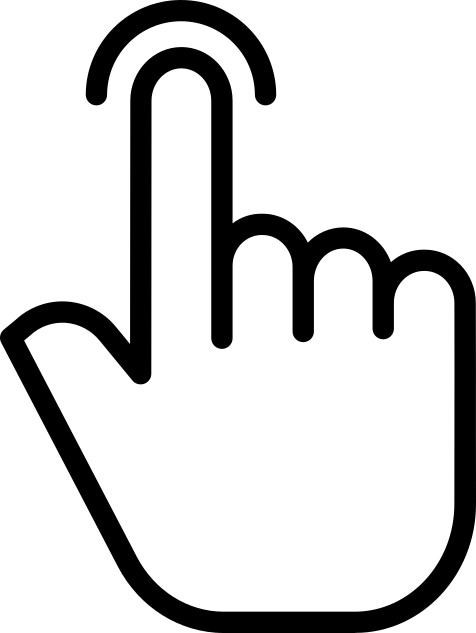
\includegraphics[width=0.10\textwidth]{static/dedo.png}} ;
    \node[const, left=of d] (nd) {\Large $s$} ;

    \edge {r} {d};
}
\caption{Modelo causal incorrecto}
\end{subfigure}
\begin{subfigure}[c]{0.49\textwidth}
\centering
\tikz{

    \node[latent] (d) {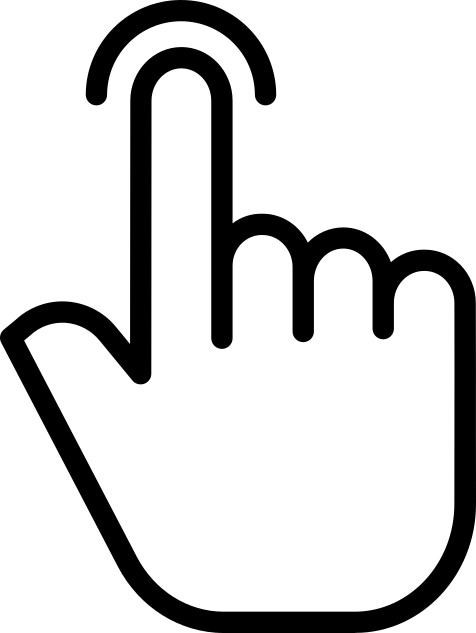
\includegraphics[width=0.10\textwidth]{static/dedo.png}} ;
    \node[const,left=of d] (nd) {\Large $s$} ;

    \node[latent, above=of d, xshift=-1.5cm] (r) {
\includegraphics[width=0.12\textwidth]{static/regalo.png}} ;
    \node[const,left=of r] (nr) {\Large $r$} ;


    \node[latent, fill=black!30, above=of d, xshift=1.5cm] (c) {
\includegraphics[width=0.12\textwidth]{static/cerradura.png}} ;
    \node[const,left=of c] (nc) {\Large $c$} ;

    \edge {r,c} {d};
}
\caption{Modelo causal correcto}
\end{subfigure}
\caption{Dos modelos causales, uno correcto y otro incorrecto.}
\end{figure}

Para simplificar el an\'alisis consideraremos que la caja elegida es siempre la 1, $c=1$.
%
Luego, en $T$ iteraciones del juego observaremos $n_{s2}$ pistas en caja 2 y $n_{s3}$ pistas en caja 3 (con $T=n_{s2} + n_{s3}$) y $n_{r1}$ regalos en caja elegida (1) y $n_{r0}$ regalos en otro caja (no 1), (con $T=n_{r1} + n_{r0}$).
%
La predicci\'on conjunta de los datos es,
\begin{align*}
P(\text{D}_{_T} = \{\overbrace{n_{s2}, n_{s3}}^{T}, \overbrace{n_{r1}, n_{r0}}^{T} \} \, | \, \text{M}) = P(s2|M)^{n_{s2}\phantom{/T}}  P(s3|M)^{n_{s3}\phantom{/T}} \, P(r1|M)^{n_{r1}\phantom{/T}} \, P(r0|M)^{n_{r0}\phantom{/T}}
\end{align*}
%
Debido a que todas las predicciones son valores entre 0 y 1, el producto de $2T$ predicciones r\'apidamente tiende a 0.
%
Para tener una intuici\'on del desempe\~no, podemos calcular la media geom\'etrica de la predicci\'on conjunta.
%
\begin{align*}
\underbrace{P(\text{D}_{_T} = \{n_{s2}, n_{s3}, n_{r1}, n_{r0}\} \, | \, \text{M})^{1/T}}_{\text{Media geom\'etrica}} = P(s2|M)^{n_{s2}/T}  P(s3|M)^{n_{s3}/T} \, P(r1|M)^{n_{r1}/T} \, P(r0|M)^{n_{r0}/T}
\end{align*}
%
La media geom\'etrica puede interpretarse como la tasa de predicci\'on de los modelos, en el sentido de que si reemplazamos cada una de las las predicciones con ese mismo valor recuperaremos la predicci\'on conjunta original.
%
Este valor var\'ia a medida que vamos observando nuevos datos, por la aleatoridad misma del proceso.
%
En el l\'imite, $T\rightarrow\infty$ las frecuencias observadas $n_{*}/T = p_*$, y el valor tiende as\'i a una constante que representa efectivamente la tasa de predicci\'on del modelo en el tiempo.
%
\begin{align*}
\overbrace{\lim_{T \rightarrow \infty} P(\text{D}|\text{M})^{1/T}}^{\text{Tasa de predicci\'on}} &= P(s2|M)^{p_{s2}} \, P(s3|M)^{p_{s3}} \, P(r1|M)^{p_{r1}} \, P(r0|M)^{p_{r0}} \\
\underbrace{\log \lim_{T \rightarrow \infty} P(\text{D}|\text{M})^{1/T}}_{\hfrac{\text{\scriptsize Tasa de predicci\'on en}}{\text{\scriptsize \'ordenes de magnitud}}} &= p_{s2} \log P(s2|M) + p_{s3} \log P(s3|M) + p_{r1} \log P(r1|M) + p_{r0} \log P(r0|M)
\end{align*}
%
En escala logar\'itmica tenemos la tasa de predicci\'on expresada en \'ordenes de magnitud.

% Parrafo

Si el modelo que estamos analizando es el correcto, el que se corresponde con la realidad, entonces las predicciones son iguales a la probabilidad de observar los datos.
%
\begin{align*}
\log \, \lim_{T \rightarrow \infty} P(\text{Datos}|\text{Modelo correcto})^{1/T} &= \sum_x p_x \log p_x = - \overbrace{\text{Entrop\'ia}}^{\hfrac{\text{\scriptsize Tasa de informaci\'on en}}{\text{\scriptsize \'ordenes de magnitud}}} \\
\log \, \lim_{T \rightarrow \infty} P(\text{Datos}|\text{Modelo incorrecto})^{1/T} &= \sum_x p_x \log p_{x|M} = - \underbrace{\text{Entrop\'ia cruzada}}_{\hfrac{\text{\scriptsize Entrop\'ia +}}{\text{\scriptsize divergencia}}}
\end{align*}
%
Donde la informaci\'on de Shannon (en \'ordenes de magnitud) se define como el negativo del logaritmo de la predicci\'on (si la predicci\'on es 0, tenemos informaci\'on infinita, si la predicci\'on es 1, tenemos informaci\'on nula) y la entrop\'ia se define como su esperanza.
%
\begin{equation*}
\overbrace{h(x) = - \log_2 P(x)}^{\text{Informaci\'on de Shannon}}  \hspace{2cm} \overbrace{H(X) = \sum_{x\in X} P(x) h(x)}^{\text{Entrop\'ia}}
\end{equation*}

% Parrafo

La tasa de predicci\'on no es m\'as que el negativo de la tasa de informaci\'on.
%
Es decir, a medida que mejoramos la predicci\'on disminuimos la cantidad de informaci\'on que obtenemos.
%
\begin{equation*}
\underset{\text{M}}{\text{arg \textbf{max}}}
\hspace{0.3cm}  \text{Predicci\'on}(\text{D}_{_T} \, | \, \text{M}) = \ \underset{\text{M}}{\text{arg \textbf{min}}} \hspace{0.3cm} \text{Informaci\'on} (\text{D}_{_T}\,|\,\text{M})
\end{equation*}

% Parrafo

Para construir un sistema de informaci\'on con la realidad (un dato de base emp\'irica metodol\'ogica) necesitamos minimizar la tasa de informaci\'on que recibimos de la realidad, maximizando la predicci\'on conjunta que hacemos de los datos (la evidencia).
%
En la siguiente secci\'on veremos c\'omo se ha construido el dato de base emp\'irica \emph{habilidad} durante el siglo 20 hasta princpios del siglo 21.


\section{Operacionalizaci\'on del dato \emph{habilidad}.}

Conocer c\'omo cambian las habilidades individuales a lo largo del tiempo es esencial en el sistema educativo y laboral.
%
Dado que son variables ocultas, lo mejor que podemos hacer es estimarlas a partir de sus consecuencias observables directas: el producto de la resoluci\'on de problemas y competencias.
%
Sin embargo la estimaci\'on de curvas de aprendiaje es tema sensible, especialmente cuando se las pretende utilizar para tomar decisiones que pueden impactar a las personas.
%
Considerar s\'olo la frecuencia de resultados positivos como indicador de la habilidad de los individuos puede conducir a aproximaciones erroneas, fundamentalmente porque su valor depende tambi\'en de la dificultad de los desaf\'ios.
%
Por esta raz\'on, todos los estimadores de habilidad ampliamente usados se basan en comparaciones por pares.
%
Desde los primeros modelos generativos, propuestos hace casi un siglo por~\cite{Thurstone1927} y~\cite{Zermelo1929}, se supone que la probabilidad de un resultado observado $r$ depende del rendimiento $p$ del agente $i$ y de su oponente $j$, expresada como $P(\, r \,|\, p_i, \, p_j \,)$.
%
El campo sigui\'o progresando con los trabajos de Bradley y Terry \cite{Bradley1952} y~\cite{Mosteller1951a,Mosteller1951b,Mosteller1951c}Mosteller, que condujeron al gran avance que tuvo lugar cuando Arpad Elo~\cite{Elo2008} desarroll\'o una metodolog\'ia para la Federaci\'on de Ajedrez de los Estados Unidos (USCF), adoptada hasta el d\'ia de hoy por la Federaci\'on Internacional de Ajedrez (FIDE).

\subsection{El estimadores de habilidad Elo: hip\'otesis indicadora ad-hoc.}

El modelo causal propuesto por Elo para estimar la habilidad de los ajedrecistas profesionales supone que las habilidades ocultas generan el resultado observable a trav\'es de desempe\~nos aleatorios.
%
\begin{figure}[ht!]
  \centering
  \begin{subfigure}[b]{0.5\textwidth}
  \centering \small
    \tikz{
    \node[det, fill=black!10] (r) {$r$} ;
    \node[const, left=of r, xshift=-1.35cm] (r_name) {\small Resultado:};
    \node[const, right=of r] (dr) {\normalsize $ r = (d > 0)$};
    \node[latent, above=of r, yshift=-0.45cm] (d) {$d$} ; %
    \node[const, right=of d] (dd) {\normalsize $ d = p_i-p_j$};
    \node[const, left=of d, xshift=-1.35cm] (d_name) {\small Diferencia:};
    \node[latent, above=of d, xshift=-0.8cm, yshift=-0.45cm] (p1) {$p_i$} ; %
    \node[latent, above=of d, xshift=0.8cm, yshift=-0.45cm] (p2) {$p_j$} ; %
    \node[const, left=of p1, xshift=-0.55cm] (p_name) {\small Desempe\~no:};
    \node[accion, above=of p1,yshift=0.3cm] (s1) {} ; %
    \node[const, right=of s1] (ds1) {$s_i$};
    \node[accion, above=of p2,yshift=0.3cm] (s2) {} ; %
    \node[const, right=of s2] (ds2) {$s_j$};
    \node[const, right=of p2] (dp2) {\normalsize $p \sim \N(s,\beta^2)$};
    \node[const, left=of s1, xshift=-.85cm] (s_name) {\small Habilidad:};
    \edge {d} {r};
    \edge {p1,p2} {d};
    \edge {s1} {p1};
    \edge {s2} {p2};

    \node[invisible, below=of r, yshift=-0.7cm] (inv) {};
  }
  \caption{}
  \label{fig:generative_model_elo}
  \end{subfigure}
  \begin{subfigure}[b]{0.375\textwidth}
      \centering
       \includegraphics[width=1\textwidth]{figures/probaOfWin_2D.pdf}
       \caption{}
     \label{fig:probaOfWin_2D}
    \end{subfigure}
     \caption{
    (\subref{fig:generative_model_elo}) Modelo generativo en el que las habilidades causan los resultados observables a trav\'es de la diferencia de rendimientos ocultos, $d=p_i-p_j$, ambas variables aleatorias centradas en la verdadera habilidad, $p \sim \N(s,\beta^2)$.
    %
    Quien haya obtenido mayor rendimiento gana, $r = (d > 0)$.
    %
    Las variables observables se pintan de gris, las ocultas en blanco, y las constantes se muestran como puntos negros.
    %
    (\subref{fig:probaOfWin_2D}) La probabilidad conjunta de los desempe\~nos.
    %
    El volumen de un lado y del otro de la diagonal representa la predicci\'on del resultado.
    }
\end{figure}
%
En su versi\'on ``Gaussiana'' (la figura~\ref{fig:generative_model_elo}, las persona exhiben distintos desempe\~nos en cada evento, que var\'ian alrededor de su verdadera habilidad, $\N(p\,|\,s,\beta^2)$.
%
El modelo supone que gana el agente con mayor desempe\~no, $r = (p_i > p_j)$.
%
El par\'ametro $\beta^2$, al ser el mismo para todos los agentes, act\'ua como la escala de las estimaciones: habilidades a una distancia de un $\beta$ implica 76\% probabilidad de ganar, independiente del valor absoluto de las estimaciones%
%
A partir de este modelo causal podemos derivar la predicci\'on a priori del resultado, $P(r|s_i^{\text{old}},s_j^{\text{old}})$.
%
En t\'erminos gr\'aficos, podemos representar esa probabilidad como el volumen indicado en la figura \ref{fig:probaOfWin_2D}.

% Parrafo

Arpad Elo propone a mediados del siglo 20 un procedimiento ad-hoc de selecci\'on de hip\'otesis sobre el valor de la variable (habilidad de los ajedrecistas) a trav\'es del indicador observado (el resultado de la partida) y el modelo causal descrito.
%
La idea es que la magnitud de la sorpresa est\'a relacionada con cuan buenas son las estimaciones previas, y por lo tanto podr\'ia usarse para actualizarlas.
%
Resultados inesperados indicar\'ian que las estimaciones actuales no son del todo correctas y deber\'ian actualizarse en mayor medida que si hubieran ocurrido como se esperaba.
%
La propuesta de Elo fue entonces utilizar la sorpresa $\Delta$ como factor de correcci\'on de las estimaciones previas.
%
\begin{equation}\label{eq:elo_update}
 s_{\text{winner}_\text{new}} = s_{\text{winner}_\text{old}} + \Delta \ \ \ \ \ s_{\text{loser}_\text{new}} = s_{\text{loser}_\text{old}} - \Delta
\end{equation}
%
Donde $\Delta$ se define como el complemento de la predicci\'on.
%
\begin{equation*}
 \Delta = \underbrace{(1 - P(r|s_i^{\text{old}},s_j^{\text{old}}))}_{\hfrac{\textbf{\footnotesize Sorpresa}}{\text{\footnotesize del resultado}}}
\end{equation*}
%
Esta es la hip\'otesis indicadora de Elo.
%
Esta soluci\'on es capaz de recuperar la escala relativa de los agentes, partiendo de valores iniciales arbitrarios.
%
\begin{center}
\tikz{ %
        \node[const] (e) {Estimaci\'on};

        \node[const, xshift=3cm] (p) {Predicci\'on};
        \node[const, xshift=1.5cm, yshift=-1cm] (s) {Sorpresa};

         \edge {e} {p};
         \edge {p} {s};
         \edge {s} {e};
}
\end{center}
%
Esta definici\'on de habilidad es usada todav\'ia hoy por la federaci\'on internacional de ajedrez (FIDE).
%
Sin embargo, el sistema Elo tiene algunas debilidades importantes.
%
La regla de actualizaci\'on (Ec.~\eqref{eq:elo_update}) es sim\'etrica, as\'i que lo que gana un agente el otro lo pierde.
%
Debido a que a los agentes nuevos comienzan con estimaciones arbitrarias (el mismo valor inicial para cualquier individuo), ellas tienden a generan alta sorpresa y por lo tanto pueden modificar bruscamente las estimaciones de sus oponentes a pesar de que ya hubieran convergido.
%
Esta debilidad ocurre por no tener en cuenta la incertidumbre sobre las estimaciones de los agentes.
%
Para resolver este problema se propuso reducir el impacto de la sorpresa en funci\'on de la cantidad de veces que el agente ha participado previamente.
%
Ese es rol que desempe\~na el K-factor usado por la FIDE, $\Delta_i = \Delta \cdot K_i$.
%
A medida que la persona tiene m\'as cantidad de partidas jugadas, el valor de K es menor.
%
De esa forma se rompe la simetr\'ia y se preserva las estimaciones de las personas que se consideran conocidas.


\subsection{TrueSkill, estimaci\'on mediante la hip\'otesis indicadora universal.} \label{sec:trueskill}

Los problemas asociados al algoritmo Elo se generan debido al uso de una hip\'otesis indicadora ad-hoc.
%
Por ello, para corregir los problemas del algoritmo Elo, en vez de seleccionar una \'unica hip\'otesis de habilidad (estimaci\'on puntual) debemos aplicar estrictamente las reglas de la probabilidad y calcular la distribuci\'on de creencia sobre todo el espacio de hip\'otesis.

% Parrafo

El m\'etodo TrueSkill~\cite{Herbrich2007} fue presentado en 2006 por Ralf Herbrich y tiene dos patentes~\cite{trueskill_patent_06, trueskill_patent_09}.
%
TrueSkill comparte el modelo de dependencia del sistema de calificaci\'on Elo entre habilidad, desempe\~no y probabilidad de ganar.
%
Lo extiende a trav\'es de un modelo bayesiano que incorpora una distribuci\'on de creencias de habilidades (el prior), y una funci\'on de actualizaci\'on no arbitraria (el posterior).

% Parrafo

Adem\'as, se extiende el modelo causal, permitiendo estimar la habilidad de los jugadores cuando participan en equipo, algo que no estaba incluido en el modelo causal original.

\subsubsection{Evidencia}

Una de las novedades de TrueSkill es la noci\'on de incertidumbre de la estimaci\'on de la habilidad.
%
La estimaci\'on de habilidad $s_i$, anteriormente representada por un escalar, ahora se representa mediante una distribuci\'on de creencias gaussiana.
%
\begin{equation}
p(s_i) = \N(s_i | \mu_i, \sigma_i^2)
\end{equation}
%
Para definir el valor a priori de la media, $\mu$, hay que recordar que el valor absoluto de habilidad no tiene ning\'un significado.
%
Lo que importa no es su valor absoluto sino la diferencia con otros jugadores: un $\beta$ de diferencia equivale a 76\% de probabilidad de ganar.
%
La incertidumbre a priori, $\sigma$, tiene ue ser lo suficientemente grande para asegurarnos de cubrir todas las posibles valores de habilidad que la persona puede tener.
%
Este valor depende del contexto.
%
En general se usa una incertidumbre que es 3 veces el desv\'io estandar del desempe\~no.

% Parrafo

Al igual que en el sistema Elo, se supone que el resultado final del juego depende del desempe\~no $p_i$ de los jugadores.
%
Sin embargo, en el modelo TrueSkill tenemos la definici\'on del desempe\~no condicional.
%
\begin{equation}
p(p_i|s_i) = \N(p_i | s_i, \beta^2)
\end{equation}
%
Para calcular el desempe\~no tenemos que integrar todos los posibles valores de habilidad.
%
En t\'erminos gr\'aficos esto es equivalente al \'area debajo de la l\'inea s\'olida en la Fig.~\ref{paso_1_multiplicacion_normales}.
%
\begin{figure}[ht!]
\centering
\begin{subfigure}[c]{0.4\textwidth}
\centering
\includegraphics[width=0.9\linewidth]{figures/Fig8}
\end{subfigure}
\begin{subfigure}[c]{0.5\textwidth}
\begin{align*}\label{p.p_i}
p(p_i) & = \int \N(p_i | s_i, \beta^2) \N(s_i | \mu_i,\sigma_i^2) ds_i  \\
&= \N(p_i|\mu_i, \beta^2 + \sigma^2)
\end{align*}
\end{subfigure}
\caption{Distribuci\'on conjunta de habilidades y desempe\~nos, calculada como el producto de la distribuci\'on de priori de las habilidad, $\N(s_i \, | \, \mu_i, \sigma_i^2)$, por la distribuci\'on condicional del desempe\~no, $\N(p_i \, | \, s_i, \beta^2)$.
%
El \'area debajo de la l\'inea s\'olida representa la probabilidad marginal de un cierto desempe\~no $p_i$.
%
La l\'inea punteada representa el valor m\'aximo.
}
\label{paso_1_multiplicacion_normales}
\end{figure}
%
Por las propiedades de la distribuci\'on gaussiana (ver anexo), esta integral se puede parametrizar usando otra gaussiana, centrada en la distribuci\'on de creencias a priori de la habilidad, $\mu$, y con la suma de incertidumbres del priori y del desempe\~no, $\N(p_i | \mu_i, \beta^2 +\sigma_i^2)$.
%
En la secci\'on~\ref{sec:2vs2} veremos en detalle c\'omo todas estas ecuaciones surgen de aplicar las reglas de las suma y el producto sobre el modelo.
%
Aqu\'i presentamos las conclusiones finales.

% Parrafo

Al igual que en el caso anterior, los desempe\~nos se expresan usando gaussianas y la probabilidad de ganar se corresponde con el volumen de un lado y del otro de la isol\'inea $p_i = p_j$ (figura~\ref{fig:probaOfWin_2D}).
%
En t\'erminos anal\'iticos, nuestra creencia a priori respecto de la diferencia de desempe\~nos, $d=p_i-p_j$, se puede expresar como una gaussiana centrada en la diferencia de las medias de las estimaciones a priori ($\mu_i - \mu_j$), con una varianza que incorpora la incertidumbre de ambas estimaciones ($\sigma$) y la varianza de ambos rendimientos ($\beta$), $\N(\, d \, | \, \mu_i -\mu_j \, ,\ 2\beta^2 + \sigma_i^2 + \sigma_j^2 \,)$.
%
Al observar que el agente $i$ gan\'o, sabemos por el modelo causal que la diferencia de desempe\~nos oculta fue en efecto positiva.
%
Por lo tanto, la predicci\'on a priori del resultado observado, o evidencia, es la densidad acumulada ($\Phi$) de todos los valores positivos de la gaussiana de diferencia de desempe\~nos (Eq.~\eqref{eq:evidence}).
%
A partir de ahora el rol del modelo se dejar\'a impl\'icito.
%
\begin{equation}\label{eq:evidence}
 \overbrace{P(r)}^{\text{Evidenc\en{e}\es{ia}}} = 1-\Phi(0 \, | \overbrace{\mu_i^{\phantom{2}} - \mu_j}^{\hfrac{\text{\en{Expected}\es{Diferencia}}}{\text{\en{difference}\es{esperada}}}} , \, \overbrace{2\beta^2 + \sigma_i^2+ \sigma_j^2}^{\hfrac{\text{\en{Total}\es{Incertidumbre}}}{\text{\en{uncertainty}\es{total}}}})
\end{equation}
%
La evidencia es una predicci\'on hecha con todas las hip\'otesis a priori.
%
% Como es constante, la incertidumbre a posteriori de cada hip\'otesis es proporcional al producto de su incertidumbre a priori y su verosimilitud, como se muestra en la ecuaci\'on~\eqref{eq:posterior_win}.

\subsubsection{Verosimilutd}

La evidencia es la verosimilitud marginal $p(r)$.
%
Para calcular el posterior sobre la habilidad $p(s_i|r)$ necesitamos la verosimilitud condicional, $p(r|s_i)$.
%
En el cap\'itulo~\ref{ch:ttt} mostramos todos los detalles que se requieren para llegar a la siguiente expresi\'on an\'al\'itica exacta.
%
\begin{equation}\label{eq:posterior_win}
\underbrace{p(\,s_i\, | \, r \, )}_{\text{Posterior}} \propto \underbrace{1-\Phi(0 \, |  s_i - \mu_j , \, 2\beta^2 + \sigma_j^2)}_{\text{\en{Likelihood}\es{Verosimilitud}} \ P(r|s_i)} \,  \underbrace{\N(s_i \, | \, \mu_i,\, \sigma_i^2)}_{\text{Prior} \ p(s_i)}
\end{equation}
%
Donde el posterior normalizado se obtiene dividiendo el lado derecho con la evidencia, $P(r)$.
%
Es interesante notar las similitudes y diferencias entre la verosimilitud y la evidencia.
%
La verosimilitud cuantifica la misma densidad acumulada que la evidencia, pero centrada ahora en la diferencia entre la hip\'otesis que estamos evaluando $s_i$ y la estimaci\'on media del oponente $\mu_j$, con una varianza que incluye todas las incertidumbres salvo la de la propia hip\'otesis $s_i$.
%
\begin{figure}[ht!]
    \centering
    \en{\includegraphics[page={1},width=.6\linewidth]{figures/posterior_win}}
    \es{\includegraphics[page={1},width=.6\linewidth]{figures/posterior_win}}
    \caption{
    %
    \en{Belief update for the winning case. }%
    \es{Actualizaci\'on de creencias para el caso ganador. }%
    %
    \en{The proportional posterior is obtained as the product of the prior (Gaussian) and the likelihood (cumulative Gaussian). }%
    \es{El posterior proporcional se obtiene como el producto de la distribuci\'on a priori (distribuci\'on gaussiana) y la verosimilitud (distribuci\'on gaussiana acumulada). }%
    %
    \en{The evidence is the integral of the proportional posterior. }%
    \es{La evidencia es la integral del posterior proporcional. }%
    %
    \en{The distributions are not necessarily on the same scale: the prior integrates to $1$, while the likelihood goes from $0$ to $1$. }%
    \es{Las distribuciones no est\'an necesariamente en la misma escala: la distribuci\'on a priori integra 1, mientras que la verosimilitud va de 0 a 1. }%
    }
    \label{fig:posterior_win}
\end{figure}

El posterior no es m\'as que la densidad del prior no filtrada por la verosimilitud.
%
La sorpresa, definida como el complemento de la verosimilitud, funciona como un filtro para el prior.
%
En la regi\'on de hip\'otesis de muy alta habilidad, donde el resultado ganador no nos hubiera generado casi ninguna sorpresa ($\lim_{s_i \to \infty}P(r|s_i) = 1$), el posterior recibe casi toda la densidad del prior.
%
En cambio, en la regi\'on de hip\'otesis de muy baja habilidad, donde el resultado habr\'ia generado mucha sorpresa ($\lim_{s_i \to -\infty}P(r|s_i) = 0$), el posterior no recibe casi nada de la densidad del prior.

% Parrafo


Esta es la estimaci\'on de habilidad correcta dado el modelo causal Elo.

\subsubsection{Posterior aproximado}

Es importante remarcar que la posterior, aunque se parezca, no es una distribuci\'on gaussiana, lo que nos impedir\'a usar la ecuaci\'on~\eqref{eq:posterior_win} iterativamente.
%
Por la forma del posterior exacto, una gaussiana puede ser usada como una buena aproximaci\'on, permiti\'endonos evitar el costo computacional de las metodolog\'ias de sampleo.
%
Uno de los principales aportes del sistema Glicko~\cite{Glikman2013} fue el desarroll\'o de un m\'etodo eficiente para aproximar la posterior exacta con una distribuci\'on gaussiana.
%
Sin embargo, este m\'etodo no garantiza que la distribuci\'on gaussiana seleccionada sea la que mejor aproxima.
%
El \'exito de la soluci\'on TrueSkill~\cite{Herbrich2007} se basa en la aplicaci\'on de m\'etodo eficiente para calcular la gaussiana que mejor aproxima al posterior exacto (secci\'on~\ref{sec:approximate_posterior}),
%
\begin{equation} \label{eq:approx}
 \widehat{p}(s_i| r, s_j) = \underset{\mu, \sigma}{\text{ arg min }} \ \ \text{KL}(\, p(s_i| r, s_j) \, || \,  \N(s_i|\mu, \sigma^2) \, )
\end{equation}
%
en t\'erminos de minizaci\'on de la divergencia Kullback-Leibler entre la distribuci\'on verdadera y la aproximada.
%
Este m\'etodo nos permite aplicar eficientemente la ecuaci\'on~\eqref{eq:posterior_win} iterativamente sobre una secuencia de observaciones, que de otra manera ser\'ia inviable.

% Parrafo

El enfoque adoptado por TrueSkill para tratar el proceso din\'amico, conocido como \emph{filtering}, usa el \'ultimo posterior aproximado como prior del siguiente evento.
%
Luego, el posterior aproximado en un determinado momento se define como,
%
\begin{equation}
 \widehat{\text{Posterior}}_t \propto \widehat{\text{Likelihood}}_t  \overbrace{\widehat{\text{Likelihood}}_{t-1} \dots \underbrace{\widehat{\text{Likelihood}}_{1} \text{Prior}_1}_{\widehat{\text{Posterior}}_{1} \text{ como } \text{Prior}_{2}} }^{\widehat{\text{Posterior}}_{t-1} \text{ \en{as}\es{como} } \text{Prior}_{t}} %= \text{Prior}_1 \prod_{i=1}^t \text{Likelihood}_i
\end{equation}
%
Donde {\footnotesize $\widehat{\text{Posterior}}_i$} y {\footnotesize $\widehat{\text{Likelihood}}_i$} representan la aproximaciones inducidas por la ecuaci\'on~\eqref{eq:approx} en el $i$-\'esimo evento.
%
Si consideramos la verosimilitud como un filtro del prior, cada posterior puede ser visto como una acumulaci\'on de todos los filtros anteriores.
%
De esta forma, la informaci\'on propaga del estimaciones pasadas hacia futuras.
%
Debido a que las habilidades cambian en el tiempo, es importante agregar alguna incertidumbre $\gamma$ luego de cada paso.
%
\begin{equation}
 \widehat{p}(s_{i_t}) = \N(s_{i_t} | \mu_{i_{t-1}}, \sigma_{i_{t-1}}^2 + \gamma^2 )
 \end{equation}
 %

\subsubsection{Modelo con equipos}

Otra de las novedades de TrueSkill fue incorporar la formaci\'on de equipos al modelo de estimaci\'on de habilidad.
%
Sea $A_e$ el conjunto de jugadores que forman parte del equipo $e$.
%
El modelo supone que el desempe\~no de un equipo es la suma de los desempe\~nos de sus miembros.
%
\begin{equation}
t_e = \sum_{j\in A_e } p_j
\end{equation}
%
El resto del modelo se preserva igual.
%
Un equipo vence a otro cuando su desempe\~no es mayor al del equipo contrario.
%
El resultado de una partida con varios equipos se modela con una desigualdad de los desempe\~nos de los equipos, tal que $t_{o_1}< \dots < t_{o_{|A|}}$, donde $o_i$ representa el equipo que qued\'o en la $i$-\'esima posici\'on.
%
En resumen, el modelo TrueSkill puede representarse mediante el siguiente modelo causal (figura~\ref{fig:modelo_trueskill_equipos}).
%


\begin{figure}[ht!]
\centering
  \scalebox{.9}{
  \tikz{ %
        \node[latent] (r) {$r_j$} ; %
        \node[const, above=of r] (dfr) {\large $\mathbb{I}(d_j>0)$}; %
        \node[latent, left=of r, xshift=-1cm] (d) {$d_j$} ; %
        \node[const, above=of d] (dfd) {\large $\delta(d_j=t_{o_j} - t_{o_{j+1}})$}; %
        \node[latent, left=of d,xshift=-2cm] (t) {$t_{o_j}$} ; %
        \node[const, above=of t,xshift=0.5cm] (dft) {\large $\delta(t_{o_j} = \sum_{i} p_i)$}; %
        \node[latent, left=of t, xshift=-0.5cm] (p) {$p_i$} ; %
        \node[const, above=of p] (dfp) {\large $\N(p_i|s_i,\beta^2)$}; %
        \node[latent, left=of p, xshift=-1cm] (s) {$s_i$} ; %
        \node[const, above=of s] (dfs) {\large $\N(s_i|\mu_i,\sigma^2)$}; %

        \edge {d} {r};
        \edge {t} {d};
	    \edge {p} {t};
        \edge {s} {p};
        \plate {personas} {(p)(s)(dfp)(dfs)} {Miembros del equipo $o_j$ \hspace{0.5cm} $i \in \text{\en{Team}\es{Equipo}}_{o_j}$}; %
        \node[invisible, below=of t, yshift=-0cm] (inv_below_e) {};
	\node[invisible, above=of t, yshift=0cm] (inv_above_e) {};
	\plate {equipos} {(personas) (t)(dft) (inv_above_e) (inv_below_e)} {$o\equiv$ lista de equipos ordenados de acuerdo al resultado  \hspace{0.3cm} $1 \leq j \leq |o|$}; %
	\node[invisible, below=of r, yshift=-0.57cm] (inv_below) {};
	\node[invisible, above=of r, yshift=0.57cm] (inv_above) {};
	\plate {comparaciones} {(dfd) (d) (dfr) (inv_below) (inv_above)} {$1 \leq j < |o|$};
    }
    }
\caption{Modelo general con equipos.
  %
  Los sub\'indices que aparecen abajo a la derecha en las placas, indican replicaci\'on.
  %
  El sub\'indice $j$ de la placa izquierda abre los $k$ desempe\~nos de equipos, y el sub\'indice $i$ de la placa interna despliega sus jugadores.
  %
  El sub\'indice $j$ de la placa derecha abre los $k-1$ comparaciones entre equipos consecutivos.
}
\label{fig:modelo_trueskill_equipos}
\end{figure}


% Parrafo

Entonces, la probabilidad del desempe\~no de un equipo integrando los desempe\~nos individuales es,
\begin{align}
 P(t_e|A_e) &= \int \dots \int \mathbb{I}(t_e = \sum_{j\in A_e } p_j ) \left(\prod_{i \in A_e} \N(p_i;\mu_i,\beta^2 + \sigma^2) \right) d\vec{p} \\
 & = \N\left(t\,|\,\sum_{i\in A_e} \mu_i,\sum_{i\in A_e} \beta^2 + \sigma_i^2\right)
\end{align}
%
Con dos equipos, la funci\'on exacta de actualizaci\'on posterior es (ver \ref{ch:ttt}),
%
\begin{equation}
 P(s_i \mid r, A) \propto
 \begin{cases}
  \N(s_i \, | \, \mu_i, \sigma_i^2) \, \Phi(0 \, | \, \delta(s_i), \vartheta - \sigma_i^2) & \text{Winning case} \\
  \N(s_i \, | \, \mu_i, \sigma_i^2 ) \, (1 - \Phi(0 \, | \, \delta(s_i), \vartheta - \sigma_i^2)) & \text{Losing case}
 \end{cases}
\end{equation}
%
donde $\delta(s_i) = \delta - \mu_i + s_i$, la diferencia esperada entre equipos reemplazando la habilidad estimada ($\mu$) por su verdadera habilidad $s_i$.
%
La soluci\'on multiequipos no tiene una forma cerrada, requiere una iteraci\'on para alcanzar convergencia que ser\'a explicada en detalle en el cap\'itulo \ref{ch:ttt}.

\subsection{Base emp\'irica metodol\'ogica \emph{habilidad}.}

El modelo de habilidad TrueSkill corrije los errores del modelo Elo a trav\'es del la evaluaci\'on bayesiana de todo el espacio de hip\'otesis.
%
Si bien en la actualidad la federaci\'on de internacional de ajedrez, y una parte de la industria del video juego sigue usando el modelo Elo por tradici\'on hist\'orica, los resultados que se obtienen con el modelo TrueSkill son ampliamente superiores.
%
El sistema Glicko~\cite{Glikman2013} es un desarroll\'o bayesiano previo, que a diferencia de TrueSkill, no garantiza que la distribuci\'on gaussiana seleccionada para aproximar al posterior exacto sea la mejor en t\'erminos de minizaci\'on de la divergencia Kullback-Leibler entre la distribuci\'on verdadera y la aproximada.

% Pararfo

Ambos modelos bayesianos de habilidad, TrueSkill y Glicko, son los elegidos por la industria del video juego, considerados como los est\'andares para estimar la habilidad de los usuarios en el tiempo.
%
Al ser los modelos m\'as ampliamente adoptados por la comunidad de los video juegos, las estimaciones de habilidad pueden ser considerada base emp\'irica metodol\'ogica sobre la cual evaluar modelos de aprendizaje.
% Parrafo
\begin{figure}[ht!]
    \centering
    \begin{subfigure}[b]{0.45\textwidth}
    \includegraphics[page=3,width=\linewidth]{figures/baseEmpirica.pdf}
    \end{subfigure}
    \caption{Niveles de base emp\'irica. En negro la base emp\'irica epistemol\'ogica, en gris la base emp\'irica metodol\'ogica, y en blanco los datos que todav\'ia no han alcanzado un acuerdo intersubjetivo amplio.}
\end{figure}
%
En cualquier caso, los resultados de las partidas son la base emp\'irica epistemol\'ogica a partir de la cual se infieren las distribuciones de creencias sobre las habilidades ocultas (no observable) de la personas.
%
Estas estimaciones de habilidad ser\'an la base emp\'irica metodol\'ogica que utilizaremos a lo largo del pr\'oximo cap\'itulo para estudiar los factores de aprendizaje social.
























\chapter{Resultado 1. Efecto de la formaci\'on de equipos sobre el aprendizaje}\label{ch:team}

El problema de la adquisici\'on de habilidades es ubicuo y fundamental para la vida.
%
La mayor\'ia de las tareas humanas se realizan en sociedad, lo que  la cooperaci\'on con otros sujetos.
%
A pesar de su importancia fundamental, la selecci\'on de compa\~neros de equipo suele pasarse por alto cuando se estudia el aprendizaje.
%
Aprovechamos el repositorio virtualmente infinito de comportamiento humano disponible en Internet para estudiar un tema relevante en la ciencia antropol\'ogica: c\'omo las estrategias de agrupaci\'on pueden afectar el aprendizaje.
%
Analizamos el impacto de las estrategias de formaci\'on de equipos en la adquisici\'on de habilidades mediante un juego por turnos donde los jugadores pueden participar individualmente o en equipos.
%
Revelamos un efecto sutil pero fuerte en la adquisici\'on de habilidades basado en la forma en que se forman y mantienen los equipos a lo largo del tiempo.
%
El \emph{``Faithfulness-boost effect''} proporciona un impulso de habilidad durante los primeros juegos que solo se adquirir\'ia despu\'es de miles de partidas de experiencia.
%
La tendencia a jugar en equipos se asocia con una mejora de las habilidades a largo plazo, mientras que jugar lealmente con el mismo compa\~nero de equipo acelera significativamente la adquisici\'on de habilidades a corto plazo.

\section{Introducci\'on}

La habilidad se adquiere principalmente a partir de la experiencia individual.
%
Sin embargo, el ser humano por sus capacidades sociales incorpora muchos de los conocimientos aprendiendo de los dem\'as.
%
El aprendizaje social puede afectar el proceso de adquisici\'on de habilidades esperado por la experiencia individual, que pueden ser tanto beneficiosas como riesgosas~\cite{Boyd2011}.
%
En este art\'iculo, aprovechamos el repositorio virtualmente infinito del comportamiento humano disponible en Internet para estudiar un tema relevante en la ciencia antropol\'ogica: c\'omo las estrategias de agrupaci\'on pueden afectar la adquisici\'on de habilidades.

% Parrafo

Las investigaciones sobre toma de decisiones expertas se iniciaron con el estudio del comportamiento de los ajedrecistas profesionales~\cite{deGroot1978-thoughtAndChoiceInChess,chase1973-perceptionInChess,simon1974-howBigIsAChunk}.
%
La experiencia individual ha sido durante mucho tiempo estudiado como el factor principal en la mejora del desempe\~no.
%
Newell se\~nal\'o en 1981 que la ley de potencia, en funci\'on del grado de pr\'actica adquirida, describ\'ia todos los datos sobre aprendizaje analizados hasta el momento~\cite{Newell1981}.
%
En los \'ultimos a\~nos, algunos autores se\~nalaron que la ley de potencia explica solamente las curvas de aprendizaje poblacionales y afirman la necesidad de proponer otras funciones para aproximar las curvas de aprendizaje individuales~\cite{heathcote2000-powerLawRepealedExponentialLawOfPractice}.
%
Sin embargo, las curvas de aprendizaje individuales son m\'as irregulares que las curvas de aprendizaje promediadas y la predicci\'on del desempe\~no a gran escala de tiempo basado en eventos de peque\~na escala de tiempo demostr\'o ser dif\'icil~\cite{howard2014-learningCurvesChessPlayersATestOfPowerLawGenerality}.
%
La pr\'actica es un factor de aprendizaje importante pero no es el \'unico.
%
Se deben tener en cuenta otros componentes esenciales para comprender mejor los procesos de aprendizaje.

% Parrafo

En los animales pro-sociales, la capacidad de aprendizaje social es un factor que modifica las curvas de aprendizaje esperadas por aprendizaje individual.
%
El aprendizaje social se define como cambios a largo plazo en el comportamiento causados por est\'imulos derivados de la observaci\'on o la interacci\'on con otros individuos~\cite{hoppitt2013-socialLearningAnIntroductionBook,bandura1977-socialLearning}.
%
Nuestra especie estuvo involucrada en una coevoluci\'on gen\'etica-cultura \'unica que provoc\'o el surgimiento de nuestras habilidades especiales de aprendizaje social: una maquinaria cognitiva costosa que permite la adquisici\'on eficiente de tradiciones complejas~\cite{Richerson2010}.
%
Los seres humanos aprendemos conocimientos de los dem\'as, los modificamos y los transmitimos a la siguiente generaci\'on, lo que lleva a una acumulaci\'on cultural que no puede ser desarrollada por un solo individuo durante su vida~\cite{boyd1985-evolutionaryProcess}.
%
La capacidad de adquirir comportamientos basados en la experiencia de otros sin tener que construirla por ensayo y error conduce a una evoluci\'on cultural acumulativa, lo que permite que las poblaciones humanas se adapten r\'apidamente a los cambios y nuevos entornos~\cite{Boyd2011}.
%
Se requiere un grado de credulidad para que este proceso funcione y, por lo tanto, los aprendices pueden adquirir informaci\'on inapropiada incluso en entornos uniformes y estables.~\cite{feldman1996-individualVsSocialLearningEvolutionaryAnalysis,giraldeau2002-potentialDisadvantagesSocialLearning}.
%
Descifrar c\'omo aprovechar la informaci\'on social mientras se manejan los inconvenientes que se derivan de su uso se ha convertido en el tema principal en la investigaci\'on sobre estrategias de aprendizaje social~\cite{henrich2003-evolutionOfCulturalEvolution,rendell2011-cognitiveCulture}.

% Parrafo

Se han propuesto muchos modelos sobre estrategias de aprendizaje social y su din\'amica de poblacional emergente.
%
Los investigadores han identificado varias estrategias te\'oricas~\cite{rendell2011-cognitiveCulture,rendell2010-socialLearningTournament}, que se puede clasificar como:
(a) aquellas que especifican las circunstancias bajo las cuales los individuos copian a otros, y
(b) aquellas que identifican de qui\'en aprenden los individuos.
%
Se han realizado muchos estudios de aprendizaje social utilizando diferentes m\'etodos, como observaciones de campo~\cite{henrich2011-adaptativeLearningBiasesFiji}, controlled laboratory experiments~\cite{mesoudi2011-experimentalPayoffBiasedSocialLearningUnderused,toelch2014-humanSocialInformationUse,caldwell2016-innovationLaboratoryCulturalEvolution,muthukrishna2016-whenAndWhoSocialLearning} y experimentos de campo~\cite{henrich2001-eco15Soc,efferson2007-learningCulturalTransmissionBolivia,wisdom2013-experiment,Glowacki2017}.
%
El aprendizaje social ahora constituye un \'area importante de estudio dentro de la biolog\'ia evolutiva y del comportamiento~\cite{mesoudi2016-individualAndCulturalVariationSocialLearning}.

% Parrafo

Todos estos m\'etodos tiene una dificultad inherente para obtener muestras de datos grandes y longitudinales.
%
Con el advenimiento de las comunidades virtuales surge la posibilidad de estudiar conjuntos de datos masivos sobre aprendizaje social correspondientes a largos per\'iodos de tiempo.
%
En este trabajo nos apoyamos en un vasto corpus ($\sim4.5$ millones de juegos), aprovechando la tendencia mundial de las personas a jugar juegos en l\'inea de varios jugadores y la existencia de servidores que acumulan datos p\'ublicos.
%
Esta novedosa metodolog\'ia busca la aparici\'on estad\'istica de efectos potencialmente sutiles, que pueden ser detectables solo con un n\'umero notable de observaciones y pueden pasar desapercibidos en tama\~nos de muestra peque\~nos t\'ipicos de los estudios de laboratorio~\cite{slezak2012-doNotFearYourOpponent}.
%
Nuestro estudio tambi\'en incorpora la capacidad actual para estimar las habilidades con alta precisi\'on.
%
Estos resultados se obtienen en condiciones experimentales \'unicas en la que los jugadores se involucran en relaciones naturales, libres de elegir a sus compa\~neros de equipo y oponentes, produciendo resultados confiables que se pueden medir directamente sin depender de m\'etodos indirectos como los cuestionarios.

% Parrafo

Los juegos en l\'inea ya se han utilizado como modelo para estudiar procesos cooperativos complejos en las ciencias sociales~\cite{Beheim2014,Johnson2009-onlineGuildsOfflineGangs}, neurociencias~\cite{slezak2012-doNotFearYourOpponent,sigman2010-chess}, y ciencias sociales computacionales~\cite{delong2013-phd_teamChemistry, shim2010-teamPerformancePrediction}.
%
El ajedrez ha sido, por su complejidad y reglas claras, un modelo privilegiado para el estudio del aprendizaje y la toma de decisiones.
%
Los datos de ajedrez masivos permitieron el an\'alisis de la influencia de la edad, las cohortes, el g\'enero y otras caracter\'isticas en el aprendizaje~\cite{chabris_glickman2006-sexDifferencesChessPerformance, roring2007-expertiseInChessAcrossLifeSpan,vaci2016-chessDatabasesAgePerformance}.

% Parrafo

Aqu\'i nos propusimos investigar el impacto de las estrategias de juego en equipo en la adquisici\'on de habilidades en \emph{Conquer Club}, un juego multijugador en l\'inea por turnos.
%
A diferencia de la naturaleza individual del ajedrez, en \emph{Conquer Club} (inspirado en el juego de mesa RISK) puede participar una cantidad variable de jugadores en cada evento, jugando individualmente o en equipos.
%
En Conquer Club hay un fuerte incentivo para la colaboraci\'on: los resultados de los juegos son por equipos.
%
Todos los miembros de un equipo ganan o pierden juntos.
%
Un jugador que es eliminado durante un juego a\'un puede terminar ganando si sus compa\~neros de equipo derrotan al resto de los equipos.
%
Por lo tanto, es fundamental que los compa\~neros de equipo puedan coordinar sus acciones.
%
A diferencia de otras plataformas, no hay contenido pago, ofreciendo las mismas condiciones para todos los jugadores.
%
No existe un mecanismo que defina la composici\'on de los equipos en funci\'on de las probabilidad de ganar de los jugadores.
%
La plataforma tiene una secci\'on ``Unirse a un juego'', donde todos los jugadores pueden ver todos los juegos abiertos.
%
Un entorno de juego t\'ipico de Conquer Club tiene cuatro elementos relevantes: el mapa actual con la ocupaci\'on de tropas en cada regi\'on, el estado del juego que muestra la ronda actual y un resumen de la informaci\'on de los jugadores, un chat p\'ublico del juego y un registro de movimientos.

% Parrafo

Los investigadores que estudian aprendizaje en ajedrez se basan en Elo, un estimador de habilidades utilizado por la Federaci\'on Mundial de Ajedrez~\cite{glickman1995-guideToChessRatings,glickman2001}.
%
Nosotros nos basamos en \emph{TrueSkill}~\cite{Herbrich2007}, una extensi\'on Bayesiana del sistema de clasificaci\'on Elo.
%
En primer lugar, TrueSkill utiliza una distribuci\'on de creencias a priori, en lugar de un escalar, para representar las estimaciones de habilidades.
%
En segundo lugar, TrueSkill modela el desempe\~no de los equipos, lo que le permite estimar la habilidad de las personas individuales a pesar de que el resultado sea el mismo para todos sus miembros.
%
Finalmente, TrueSkill utiliza una funci\'on de actualizaci\'on no arbitraria, el posterior del modelo bayesiano, que se calcula marginalizando la distribuci\'on conjunta~\cite{Kschischang2001}.
%
Como resultado, TrueSkill puede identificar con precisi\'on la habilidad de los jugadores con la menor cantidad de partidas posibles.

% Parrafo

Con nuestro enorme conjunto de datos, podemos investigar el impacto de las estrategias de juego en equipo en la adquisici\'on de habilidades individuales que, de otro modo, no ser\'ia posible estudiar.

\section{La ley de la pr\'actica}

Primero, estudiamos c\'omo las personas mejoran su desempe\~no a medida que ganan experiencia, es decir, la ley de la pr\'actica.
%
Estimamos la experiencia de cada jugador por el n\'umero de partidas jugadas.
%
La habilidad se estima seg\'un el m\'etodo \emph{TrueSkill}~\cite{Herbrich2007}.
%
La diferencia de habilidad entre los oponentes indica con alta precisi\'on la probabilidad de ganar.
%
Con dos oponentes (equipos o individuos), la probabilidad de ganar cuando el otro tiene la misma habilidad es $1/2$ y una diferencia de $4$~tsp (puntos TrueSkill) aumenta la probabilidad de ganar a $2/3$~tsp.

% Parrafo

En nuestro contexto, la curva de aprendizaje es la progresi\'on de habilidades a medida que se adquiere experiencia (es decir, la cantidad de partidas jugadas).
%
Como se mencion\'o, las curvas de aprendizaje de la poblaci\'on deben seguir una funci\'on de ley de potencia~\cite{Newell1981},
%
\begin{equation}\label{lawOfPractice}
   \text{\emph{habilidad}} = \text{\emph{habilidad}}_0 \cdot \text{\emph{Experiencia}}^{\alpha}
\end{equation}
%
donde $\alpha$ es la tasa de aprendizaje caracter\'istica de la poblaci\'on y \emph{Skill}$_0$ la habilidad de la poblaci\'on despu\'es del primer juego.

% Parrafo

Para analizar la ley de la pr\'actica, dividimos a los jugadores seg\'un su actividad total: (1) jugadores con al menos $8$ partidas y menos de $16$, (2) jugadores al menos $16$ partidas y menos de $32$, etc.
%
Por lo tanto, ajustamos los par\'ametros de la ley de la pr\'actica a cada uno de los conjuntos de jugadores seg\'un su nivel de actividad.
%
De acuerdo con la ley de la pr\'actica, observamos una dependencia lineal en las curvas de aprendizaje en escala logar\'itmica en todos los segmentos poblacionales~(Figura~\ref{learningskill_curve}).

\begin{figure}[ht!]
\centering
\includegraphics[width=.49\linewidth]{figures/Fig1}
\caption{
Ley de la pr\'actica.
%
Curva de aprendizaje de la subpoblaciones de jugadores seg\'un su nivel actividad total.
%
Cada curva de aprendizaje muestra la habilidad de los primeros $2^n$ partidas jugadas de la subpoblaci\'on con al menos $2^n$ partidas jugadas y menos de $2^{n+1}$.
%
Las subfiguras muestran los valores de los parametros (es decir, $\alpha$ y \emph{Skill}$_0$) de cada curva de aprendizaje siguiendo la ecuaci\'on~\ref{lawOfPractice}.
}
\label{learningskill_curve}
\end{figure}

Las curvas de aprendizaje dependen del abandono, exhibi\'endose una habilidad m\'as baja para las subpoblaciones con una actividad total m\'as baja.
%
Sin embargo, la tasa de aprendizaje ($\alpha$) se mantiene estable para las subpoblaciones con al menos $32$ de partidas jugadas (subfigura superior derecha en~\ref{learningskill_curve}).
%
La diferencia entre ellos causa poca variaci\'on en la adquisici\'on de habilidades a largo plazo, con menos de $0.24$~tsp despu\'es de $1000$ partidas jugadas.
%
La habilidad de inicial de la subpoblaci\'on ($Skill_0$) tambi\'en se ve afectada por el abandono (subfigura abajo a la izquierda en~\ref{learningskill_curve}).
%
Sin embargo, todas las subpoblaciones con al menos $64$ juegos jugados, no tienen una habilidad inicial significativamente diferente (Wilcoxon rank-sum test en Anexo).

% Parrafo

Por lo tanto, todas las cohortes con al menos $64$ partidas jugadas tienen curvas de aprendizaje casi equivalentes.
%
Son lo que llamamos la ``curva de aprendizaje esperada por la experiencia''.
%
Este aprendizaje b\'asico puede verse alterado por muchos factores.
%
Por ejemplo, el compromiso de terminar los juegos es sin duda un factor relevante en el proceso de adquisici\'on de habilidades.
%
De hecho, los jugadores que siempre terminan sus juegos tienen una curva de aprendizaje m\'as alta que el resto de la poblaci\'on, alrededor de $0.5$~tsp (Fig.~\ref{learningskill_comprometidos} Anexo).

\section{Aprendizaje social}

El aprendizaje social es esencial para los animales prosociales.
%
Nuestra hip\'otesis es que la curva de aprendizaje esperada por la experiencia individual podr\'ia verse alterada por diferentes comportamientos de agrupaci\'on.
%
Para estudiarlo, analizamos el comportamiento de los jugadores en la selecci\'on de equipos.

% Parrafo

En la plataforma de juego, los usuarios pueden elegir entre jugar individualmente o en equipos.
%
Definimos el concepto \emph{Team-oriented behavior} (TOB) de los jugadores como el n\'umero de partidas en las que participa de un equipo dividido por el n\'umero total de partidas jugadas:
%
\begin{equation}
\text{\emph{Team-oriented behavior}} = \frac{\text{\emph{Partidas de equipo jugadas}}}{\text{\emph{Partidas jugadas}}}
\end{equation}
%
Para evaluar la influencia de TOB en las curvas de aprendizaje, dividimos la poblaci\'on en TOB fuerte, medio y d\'ebil (es decir, $0.8<\text{\emph{TOB}}\leq 1$, $0.4 <\text{\emph{TOB}}\ leq 0,6$ y $0 <\text{\emph{TOB}}\leq 0.2$, respectivamente).
%
En adelante, excluimos a los jugadores con menos de cuatro partidas en equipo.

% Parrafo

En el largo plazo, entre $200$ y $500$ juegos de experiencia, las curvas de aprendizaje se ordenan seg\'un su nivel de TOB, exhibiendo un mayor nivel de habilidad para las poblaciones con mayor TOB (Figura~\ref{learningskill_team_hasta4team}).
%
Los jugadores TOB altos muestran, despu\'es de $250$ partidas, una habilidad final significativamente m\'as alta en comparaci\'on con TOB medio y d\'ebil (Wilcoxon rank-sum test, $p<1 \times10^{-4}$).

% Parrafo

En este intervalo, la poblaci\'on de TOB fuerte y media est\'a distanciada por alrededor de $1$~tps.
%
Un comportamiento TOB alto adquiere, a largo plazo, un mayor valor de habilidad incluso en comparaci\'on con jugadores sin juegos de equipo.


\begin{figure}[ht!]
\centering
\includegraphics[width=.49\linewidth]{figures/Fig2}
\caption{
Aprendizaje social.
%
La curva de aprendizaje para TOB fuerte, medio y d\'ebil.
%
La banda representa el intervalo de confianza de $95\%$ del Wilcoxon rank-sum y la l\'inea central representa la pseudomediana.
%
Como referencia, mostramos la curva de aprendizaje de toda la poblaci\'on.
%
Los resultados son an\'alogos a los obtenidos con la media y el intervalo de confianza de $95\%$ del t-test.
}
\label{learningskill_team_hasta4team}
\end{figure}


\subsection{Faithfulness-boost effect}

Los jugadores pueden elegir entre jugar con el mismo compa\~nero de equipo o seleccionar diferentes jugadores en cada juego.
%
Nuestra hip\'otesis es que un comportamiento leal puede afectar el aprendizaje (aumentar o disminuir la tasa de adquisici\'on de habilidades) cuando se juega en equipo.
%
La mayor\'ia de las veces que dos personas aparecen recurrentemente en la misma partida vemos que la inmensa mayor\'ia las personas son compa\~neras de equipo en lugar de oponentes.
%
Por lo tanto, enfocamos nuestro an\'alisis solo en la lealtad de los compa\~neros de equipo ya que la lealtad en los oponentes no est\'a presente en nuestra base de datos.
%
Definimos el concepto \emph{loyalty} de las personas como la proporci\'on de veces que juegan con el compa\~nero de equipo m\'as recurrente dividida por la cantidad de partidas de equipo jugadas:
%
\begin{equation}
\text{\emph{Loyalty}} = \frac{\text{\emph{M\'aximo de partidas jugadas con un mismo compa\~nero}}}{\text{\emph{Partidas de equipo jugadas}}}
\end{equation}
%
Para evaluar la influencia del loyalty sobre el aprendizaje, examinamos la evoluci\'on de las habilidades de los jugadores con TOB fuerte en funci\'on de su valor de loyalty.
%
Definimos un jugador como \emph{leal} cuando $\text{\emph{loyalty}}>0.5$, y un jugador como \emph{casual} cuando $\text{\emph{loyalty}}\leq 0.2$.

% Parrafo

Si comparamos las curvas de aprendizaje de jugadores leales y casuales, obtenemos una separaci\'on sustancial entre ellos en los primeros juegos de experiencia.
%
Los jugadores leales muestran un incremento en la habilidad media de aproximadamente $4$~tsp sobre los jugadores casuales (Fig.~\ref{learningskill_pteam89_ployal}).
%
La distribuci\'on de habilidades en cada punto de la curva de aprendizaje es significativamente diferente hasta $386$ partidas jugadas (Wilcoxon rank-sum test $p<0.01$).
%
Un comportamiento an\'alogo entre las subclases leales y casuales ocurre tambi\'en para los TOB medios y d\'ebiles(Fig.~\ref{learning_curve_ployal_hasta4team_longRun} en Anexo), aunque menos intensos ya que est\'an menos orientados a equipos.

% Parrafo

Para estudiar la interacci\'on entre TOB y loyalty en la adquisici\'on de habilidades, fijamos el n\'umero de juegos jugados en $100$.
%
Al aislar esta interacci\'on (sin la interferencia de la experiencia) encontramos que un aumento en loyalty siempre implica un aumento en la habilidad, m\'as prominente para valores m\'as altos de TOB (Fig.~\ref{skillModels_loyaltyTeamOriented_imageEmpirical}).
%
Por el contrario, el aumento de los valores de TOB muestra una disminuci\'on de la habilidad para los niveles bajos de loyalty, y solo implica un aumento de la habilidad para los niveles altos de loyalty.
%
La diferencia de habilidad del m\'inimo al m\'aximo es mayor a $4.5$~tsp.

\clearpage
\begin{figure}[ht!]
\centering
\includegraphics[width=.49\linewidth]{figures/Fig3}
\caption{
Curvas de aprendizaje de las subclases leal y casual de la clase TOB fuerte.
%
La banda representa el intervalo de confianza 95\% Wilcoxon rank-sum, y la l\'inea media representa la pseudomediana.
%
Como referencia, mostramos la curva de aprendizaje de toda la poblaci\'on y la clase TOB fuerte.
%
Los resultados son an\'alogos a los obtenidos con la media y el intervalo de confianza 95\% t-test.
%
La l\'inea vertical en $100$ partidas jugadas indica el an\'alisis realizado en la Fig.~\protect\ref{skillModels_loyaltyTeamOriented_imageEmpirical}.
}
\label{learningskill_pteam89_ployal}
\end{figure}

\begin{figure}[ht!]
\centering
\includegraphics[width=.49\linewidth]{figures/Fig4}
\caption{
Interacci\'on de la habilidades entre loyalty y TOB para todos los jugadores.
%
El papel de la experiencia se aisl\'o tomando la habilidad de los jugadores en el mismo punto de la experiencia.
%
Todos los jugadores tienen $100$ de partidas jugadas.
%
La habilidad promedio de cada parcela se informa mediante la escala de grises.
%
Se muestran las curvas de nivel.
%
Las parcelas vac\'ias tienen menos de cinco jugadores.
}
\label{skillModels_loyaltyTeamOriented_imageEmpirical}
\end{figure}

La interacci\'on entre loyalty y TOB se puede resumir como $ \text{\emph{Loyalty}} \cdot \text{\emph{TOB}} = \text{\emph{faithfulness}}$, lo que queda definido como,
%
\begin{equation}
\text{\emph{Faithfulness}} = \frac{\text{\emph{M\'aximo de partidas jugadas con un mismo compa\~nero}}}{\text{\emph{Partidas jugadas}}}
\end{equation}
%
que es simplemente la proporci\'on de veces jugadas con el compa\~nero de equipo m\'as leal sobre todos las partidas jugadas.

% Parrafo

Para medir la influencia sobre la adquisici\'on de habilidades de loyalty, TOB and faithfulness, construimos un modelo lineal que ser\'a resuelto por m\'inimos cuadrados.
%
La correlaci\'on entre las variables loyalty y TOB es baja ($0,11$) y Variance Inflation Factor es nulo ($1,01$), lo que sugiere que no hay evidencia de colinealidad.

\begin{equation}
\text{skill}_i \sim \beta_1\text{loyalty}_i + \beta_2\text{TOB}_i + \beta_3\text{faithfulness}_i
\end{equation}

Con $100$ partidas jugadas, la variable loyalty tiene una pendiente positiva significativa, la variable TOB tiene una negativa significativa, mientras que la variable faithfulness tiene una pendiente positiva pronunciada significativa (Table~\ref{model}).
%
La variable faithfulness es lo suficientemente fuerte como para revertir la contribuci\'on negativa de TOB sobre la habilidad a una positiva cuando $\text{\emph{loyalty}}>0.27$.
%
El \emph{faithfulness-boost effect} es de alrededor de $3.7$~tsp, lo que genera una diferencia de habilidades entre jugadores con la misma experiencia extremadamente relevante en t\'erminos de probabilidad de ganar.

\begin{table}[ht]
\centering
\begin{tabular}{rrrrl}
  \hline
 & Estimate & Std. Error & t value & Pr($>|t|$) \\
  \hline
Intercept & 28.5707 & 0.0405 & 705.59 & $p< 2e^{-16}$ \\
  Loyalty & 0.7594 & 0.0972 & 7.82 & $p< 2e^{-14}$ \\
  Team-oriented & -1.0042 & 0.1088 & -9.23 & $p< 2e^{-16}$ \\
  Faithfulness & 3.7077 & 0.2611 & 14.20 & $p< 2e^{-16}$ \\
   \hline
\end{tabular}
\caption{
Influencia sobre el aprendizaje de las variables de loyalty, TOB and faithfulness (modelo lineal). Reportamos el valor de la pendiente estimada, su desviaci\'on est\'andar y la significatividad respecto a una pendiente cero. Todos los jugadores tienen juegos de $100$ de experiencia.
}
\label{model}
\end{table}

Repetimos este procedimiento para jugadores con la misma experiencia, a partir de $100$ a $1300$ partidas jugadas (Fig.~\ref{skillModels_loyaltyTeamOriented_parameterGifFitted} en Anexo).
%
El \emph{faithfulness-boost effect} sigue siendo significativo hasta $400$ partidas jugadas, siempre por encima de $3$~tsp.
%
A partir de $500$ partidas jugadas, la variable faithfulness deja de ser significativa pero la pendiente de la variable TOB revierte su contribuci\'on a una significativa positiva.
%
La variable loyalty tiene un efecto positivo significativo en cualquier nivel de experiencia ($\geq 100$ partidas jugadas).
%
Aunque el efecto de interacci\'on del modelo lineal (faithfulness) ya no es significativo a partir de $500$ partidas de experiencia, el punto de m\'axima habilidad siempre se alcanza maximizando tanto la variable loyalty y TOB.
%
La magnitud de esta contribuci\'on siempre es relevante en t\'erminos de probabilidad de ganar, con m\'as de $2$~tsp.

% Parrafo

Para integrar todas las observaciones parciales realizadas hasta aqu\'i, realizamos un modelo general ajustado a todos los datos, incluyendo la experiencia, loyalty y TOB como predictores y la identidad de la persona como efecto aleatorio (Table~\ref{lmm}).
%
Elegimos un modelo mixto lineal porque la relaci\'on entre la experiencia y la habilidad es lineal en una escala logar\'itmica (Eq.~\ref{lawOfPractice}).
%
La variable dependiente, habilidad de los jugadores, se transform\'o a una escala logar\'itmica,

\begin{center}
$\text{log$_{10}$(\emph{skill})} = \text{log$_{10}$(\emph{experience})} + \text{\emph{loyalty}} + \text{\emph{TOB}} + \text{\emph{individual player}} + \varepsilon$
\end{center}

El conjunto de datos utilizado contiene los valores para todos los jugadores entre $10$ y $500$ partidas jugadas.
%
La colinealidad entre variables es nula en t\'erminos del Variance Inflation Factor calculado a partir de un modelo lineal resuelto por m\'inimos cuadrados (es decir, todos los VIF son inferiores a $1.5$).
%
Por tanto, podemos ajustar el modelo lineal sin incurrir en resultados artificiales.

\begin{table}[ht!]
\centering
\begin{tabular}{rrrrrr}

 & Estimate & Norm.Est. & t value  & [0.005 & 0.995] \\
  \hline
Intercept               &  1.415  &  26.00   & 5966.264  &  1.414 &  1.415 \\
exp           		&  0.016  &   0.98   &  225.628  &  0.016 &  0.017 \\
loyal         		& -0.007  &  -0.42   &  -28.846  & -0.008 & -0.006 \\
tob           		& -0.044  &  -2.51   &  -91.773  & -0.045 & -0.043 \\
(faithful) loyal:tob    &  0.090  &   5.99   &   91.801  &  0.088 &  0.093 \\
exp:tob       		&  0.016  &   0.98   &   70.829  &  0.015 &  0.016 \\
exp:loyal     		&  0.004  &   0.24   &   29.678  &  0.003 &  0.004 \\
exp:loyal:tob 		& -0.026  &  -1.51   &  -56.129  & -0.027 & -0.025 \\
Group Var     		&  0.002  &          &           &        &       \\
   \hline
\end{tabular}
\caption{
Modelo mixto lineal para ajustado para todos los datos entre 10 y 500 partidas jugadas de experiencia individual.
%
En la columna Norm.Est. transformamos los estimadores, en escala logar\'itmica, a su valor normalizado (e.g. $\text{Intercept} = 10^{1.415}$, $\text{exp} = 10^{1.415+0.016} - 10^{1.415}$).
%
M\'etodo: REML converged. N\'umero de grupos: $65335$. Tama\~no m\'aximo de grupo: $491$. Tama\~no medio de grupos: $99.5$}
\label{lmm}
\end{table}

Este modelo general confirma las observaciones ya introducidas.
%
La experiencia es el principal predictor en cuanto a su nivel de significatividad, tiene la pendiente m\'as significativa.
%
Inicialmente, la variable loyalty solo tiene un efecto positivo en contextos de orientados a equipos (loyal:tob).
%
Ser leal sin un comportamiento orientado a equipo tiene un efecto muy marginal (loyal).
%
Sin un compa\~nero de equipo estable, jugar en equipos es un mal plan (tob).
%
Sin embargo a medida que se gana mayor experiencia, y el efecto de la interacci\'on faithfulness pierde fuerza (exp:loyal:tob), el efecto de la variable loyalty (exp:loyal) y TOB (exp:tob) revierten su contribuci\'on a una positiva.
%
Debido a esta din\'amica el valor m\'aximo de habilidad se alcanza siempre cuando se maximizan ambas variables TOB y loyalty, es decir maximizando el faithfulness.

\section{Discusi\'on}

Tradicionalmente el aprendizaje ha sido modelado en funci\'on de la experiencia.
%
En este art\'iculo nos enfocamos en c\'omo la curva de aprendizaje esperada por la experiencia individual se ve alterada por diferentes estrategias de agrupamiento.
%
Nuestro m\'etodo se basa en datos masivos que permitieron realizar un estudio longitudinal con una precisi\'on muy alta para detectar cambios sutiles.

% Parrafo

Analizamos el aprendizaje en un contexto competitivo.
%
En este tipo de juegos el aprendizaje se mide en t\'erminos de la probabilidad de ganar a otras personas.
%
A diferencia de las tareas en las que se puede determinar la cantidad absoluta de errores que comete un individuo al resolverla, en los juegos competitivos la probabilidad de ganar es una propiedad relativa que depende del nivel de aprendizaje de los oponentes.
%
Las curvas de aprendizaje derivadas de tareas en las que la habilidad se mide en t\'erminos relativos son m\'as vol\'atiles que las medidas en t\'erminos absolutos.
%
Por lo tanto, las curvas de aprendizaje individuales de los jugadores que compiten a veces son dif\'iciles de ajustar~\cite{howard2014-learningCurvesChessPlayersATestOfPowerLawGenerality,Gaschler2014}.

% Parrafo

Si bien las curvas de aprendizaje individual son m\'as irregulares que el promedio de un conjunto de curvas de aprendizaje, la variaci\'on entre ellas debe ser explicada.
%
Nuestra hip\'otesis para explicar las variaciones observadas afirma que el aprendizaje social produce un efecto de segundo orden en la adquisici\'on de habilidades.
%
Seg\'un las teor\'ias del aprendizaje social, los jugadores tienen dos opciones para aprender: i) descubrir por s\'i mismos las claves para jugar mejor; o ii) imitar la estrategia de otros disponibles en su red.
%
Nos basamos en el juego en l\'inea Conquer Club porque, a diferencia del ajedrez, se puede jugar en equipos.
%
En Conquer Club tanto los oponentes como los compa\~neros de equipo son observables y, en consecuencia, son modelos a imitar.
%
Sin embargo, enfocamos nuestro an\'alisis solo en la lealtad de los compa\~neros de equipo ya que la lealtad en los oponentes no est\'a presente en nuestra base de datos.

% Parrafo

Por ejemplo, una estrategia de aprendizaje social simple consiste en copiar la mayor\'ia de los otros modelos disponibles, lo que se conoce como \emph{frequency-based strategy}.
%
Otra estrategia de aprendizaje social es copiar el modelo disponible m\'as exitoso, denominado como \emph{payoff-based strategy}.
%
Hasta donde sabemos, no se ha propuesto ninguna estrategia de aprendizaje social que tenga en cuenta diferentes estrategias de agrupaci\'on.
%
Encontramos que las estrategias de agrupaci\'on afectan significativamente c\'omo se adquiere la habilidad.

% Parrafo

Se sabe que el \'exito de nuestra especie depende de la formaci\'on de grupos~\cite{Richerson2010,dunbar1993-coevolutionNeocorticalSizeGroupSizeAndLanguage}.
%
Aqu\'i exploramos en qu\'e medida este comportamiento afecta la adquisici\'on de habilidades utilizando un entorno controlado: Conquer Club.
%
Hemos visto que la decisi\'on de jugar en equipos est\'a asociada con una mejora de habilidades a largo plazo.
%
Encontramos que la tendencia a jugar en grupos (el n\'umero de partidas jugadas en equipo dividido por el n\'umero total de partidas jugadas) mejora significativamente el nivel de habilidad alcanzado.

% Parrafo

Los modelos matem\'aticos muestran que las estrategias adaptadas a entornos distintos a los actuales (e.g. migraci\'on) puede ser un factor de riesgo para el aprendizaje social~\cite{boyd1989-socialLearningAsAdaptation}.
%
Estudiamos una versi\'on reducida de la migraci\'on entre grupos analizando c\'omo los jugadores repiten compa\~neros de equipo, lo que conduce a una estabilidad intragrupal (i.e.~loyalty).
%
Siguiendo la teor\'ia del riesgo del cambio ambiental, afirmamos que no hay modificaciones ambientales en Conquer Club y, por lo tanto, la movilidad intergrupal no es una fuente para la difusi\'on de ideas mal adaptativas.
%
Por el contrario, la migraci\'on implicar\'ia el acceso a diferentes grupos y, por lo tanto, aprender de diferentes jugadores y aumentar las habilidades al aprender de una mayor variedad de compa\~neros de equipo.
%
En este sentido, lo que esper\'abamos encontrar era que este tipo de migraci\'on sea beneficiosa para mejorar el aprendizaje.
%
Sin embargo encontramos lo opuesto.

% Parrafo

Primero, verificamos la ley de la pr\'actica en nuestro conjunto de datos.
%
% Encontramos la forma emp\'irica de lo que llamamos la ``curva de aprendizaje esperada por la experiencia''.
%
Tom\'andolo como \emph{baseline}, cuantificamos en qu\'e medida los diferentes comportamientos de agrupamiento alteran la adquisici\'on de habilidades esperadas por la experiencia.
%
Encontramos que un comportamiento orientado a equipo est\'a relacionado con una mejora significativa del nivel de habilidad a largo plazo.
%
Una tendencia de estabilidad dentro del grupo (la lealtad) se asocia con una r\'apida mejora de las habilidades a corto plazo.
%
La combinaci\'on de estos dos efectos puede ser aprovechado para el aprendizaje.
%
El \emph{faithfulness-boost effect} proporciona un impulso de habilidad que se adquirir\'ia, a trav\'es de la experiencia, solo despu\'es de miles de partidas de pr\'actica.

% Parrafo

Afirmamos que la habilidad actual del compa\~nero de equipo puede ser ignorada.
%
No se observan efectos secundarios derivados de la heterogeneidad de habilidades entre los compa\~neros de equipo.
%
La probabilidad de victoria de un equipo es independiente de la diferencia entre compa\~neros (Fig.~\ref{fig:trueskillDimorphismMaxMin_ProbWin} en Anexo).
%
Tambi\'en es importante se\~nalar que ser parte de un equipo con pocas probabilidades de ganar no significa perder la habilidad.
%
Asociarse con un compa\~nero de equipo con menos habilidades implicar\'a efectivamente una disminuci\'on en la probabilidad de ganar, pero no necesariamente implicar\'a una disminuci\'on en la habilidad.
%
Si la colaboraci\'on es s\'olida, ambos jugadores se beneficiar\'an del efecto positivo sobre la adquisici\'on de habilidades.

% Parrafo

La evidencia deja importantes preguntas abiertas que pueden tener implicaciones pr\'acticas para la planificaci\'on de estrategias de capacitaci\'on.
%
Nuestra hip\'otesis sugiere que la sociabilidad es el factor de aprendizaje subyacente de diferentes t\'acticas de agrupaci\'on.
%
Sin embargo, se necesita m\'as trabajo para poder formular explicaciones y recomendaciones confiables.
%
La investigaci\'on experimental es necesaria para determinar con certeza las causas de esos efectos observados.
%
Creemos que el efecto positivo de la asociaci\'on surge del compromiso social.
%
Los derivados sociocognitivos de la lealtad como la confianza, la constancia y la comunicaci\'on fluida superan los costes de coordinaci\'on y la reducci\'on del abanico de relaciones que se pueden establecer.


\section{Materiales y m\'etodos}

Todos los juegos se descargaron de Conquer Club, un servicio gratuito que ofrece jugar juegos tipo RISK.
%
El sitio web permite a cualquier persona, y no solo a los participantes registrados, explorar los partidos y buscar sus datos relacionados.
%
Los usuarios registrados se identifican por sus apodos y, para ser aceptados como usuarios, deben aceptar que sus partidas se almacenen en un servidor de acceso p\'ublico.
%
Adem\'as, durante el proceso de descarga, cada jugador fue identificado por un n\'umero de identificaci\'on interno, anonimizando los datos.
%
En consecuencia, no fue necesario el consentimiento individual debido a esta doble capa de anonimato y la naturaleza abierta del sitio web.
%
Nos comunicamos con los propietarios de Conquer Club para obtener la autorizaci\'on para realizar este proceso, cumpliendo as\'i con los t\'erminos de uso de este sitio.

% Parrafo

La aplicaci\'on consta de un script \texttt{Python} que se conecta al servidor de Conquer Club.
%
Los datos entre $2006/01/03$ y $2009/07/12$ se almacenan en una base de datos \texttt{PostgreSQL}.
Hay cerca de $4.4$ millones de partidas jugadas por casi $270$ mil usuarios diferentes.

Para calcular la habilidad, usamos el paquete \texttt{TrueSkill 0.4.4} de \texttt{Python}.
%
Todos los jugadores comienzan con una habilidad media $\mu = 25$ y una desviaci\'on est\'andar de habilidad de $\sigma = 8,33$.
%
El valor de probabilidad de empate se estableci\'o en 0 ya que no hay posibilidad de empate en Conquer Club.

\subsection{La plataforma}

\paragraph{Gameplay}\label{sub:gameplay}

Al comienzo de cada partida, las regiones del mapa se distribuyen aleatoriamente entre los jugadores a las que le asignan una cierta cantidad de tropas.
%
Cada turno consiste en i) desplegar nuevas tropas, ii) asaltar las regiones vecinas del oponente y iii) reforzar las regiones.
%
El entorno del juego tiene cuatro elementos relevantes: el tablero actual, un panel con el estado del juego, un chat p\'ublico y un registro de movimientos (Fig.~\ref{conquerImage}).

% Parrafo

En este ejemplo, se juega una partida de dos equipos en equipos de dos jugadores.
%
Los nodos del gr\'afico representan las regiones, el color indica a qui\'en pertenece, los n\'umeros representan el n\'umero de tropas y las formas indican la agrupaci\'on de regiones por zonas.
%
Al lado hay un panel con el n\'umero de ronda, el jugador activo y el tiempo restante para jugar la ronda actual, y un resumen de las tropas totales y las regiones controladas totales para cada jugador.
%
El color junto al apodo identifica el n\'umero total de regiones que tiene cada jugador en el mapa.
%
Un servicio de chat p\'ublico est\'a disponible dentro de cada juego.
%
El Log registra todos los movimientos de los jugadores.

% Parrafo

Al comienzo de cada turno, los jugadores ganan nuevas tropas.
%
La cantidad de tropas resulta del n\'umero de \emph{regions} ocupadas y la bonificaci\'on de la \emph{zone} controlada y eventualmente por el intercambio de \emph{spoils} (Section A en Anexo).
%
Podemos ver en la primera l\'inea del Log en la Fig.~\ref{conquerImage}d que el jugador $c$ recibi\'o tropas por mantener el Continente 4.
%
Estas tropas pueden desplegarse en sus regiones ocupadas.
%
Por ejemplo, el jugador $c$ despliega todas sus tropas en la regi\'on $M$.

% Parrafo

Una vez finalizado el despliegue comienza la fase de asalto.
%
Un jugador puede asaltar la regi\'on de cualquier oponente siempre que ambas est\'en adyacentes y la regi\'on asaltante tenga un m\'inimo de dos tropas.
%
El motor del juego tira un dado por cada tropa que asalta, excepto por una tropa que necesita permanecer en la regi\'on, hasta un m\'aximo de tres tropas.
%
Luego, el sistema lanza un dado por cada tropa defensora, hasta un m\'aximo de dos tropas.
%
Los valores obtenidos de cada lado se ordenan de forma creciente y luego se comparan uno por uno.
%
Si el dado de asalto es m\'as alto, la regi\'on defensora pierde una tropa.
%
Si el dado defensor es mayor o igual, la regi\'on atacante pierde una tropa.
%
Si el atacante destruye todas las tropas defensoras, algunas de las tropas restantes deben moverse para ocupar la regi\'on reci\'en conquistada.
%
In our example, player $c$ assaults region $N$ from region $M$ and conquers it from player $a$.
%
Luego, este jugador usa las tropas movidas recientemente para conquistar otra regi\'on.

\begin{figure}[ht!]
    \centering
    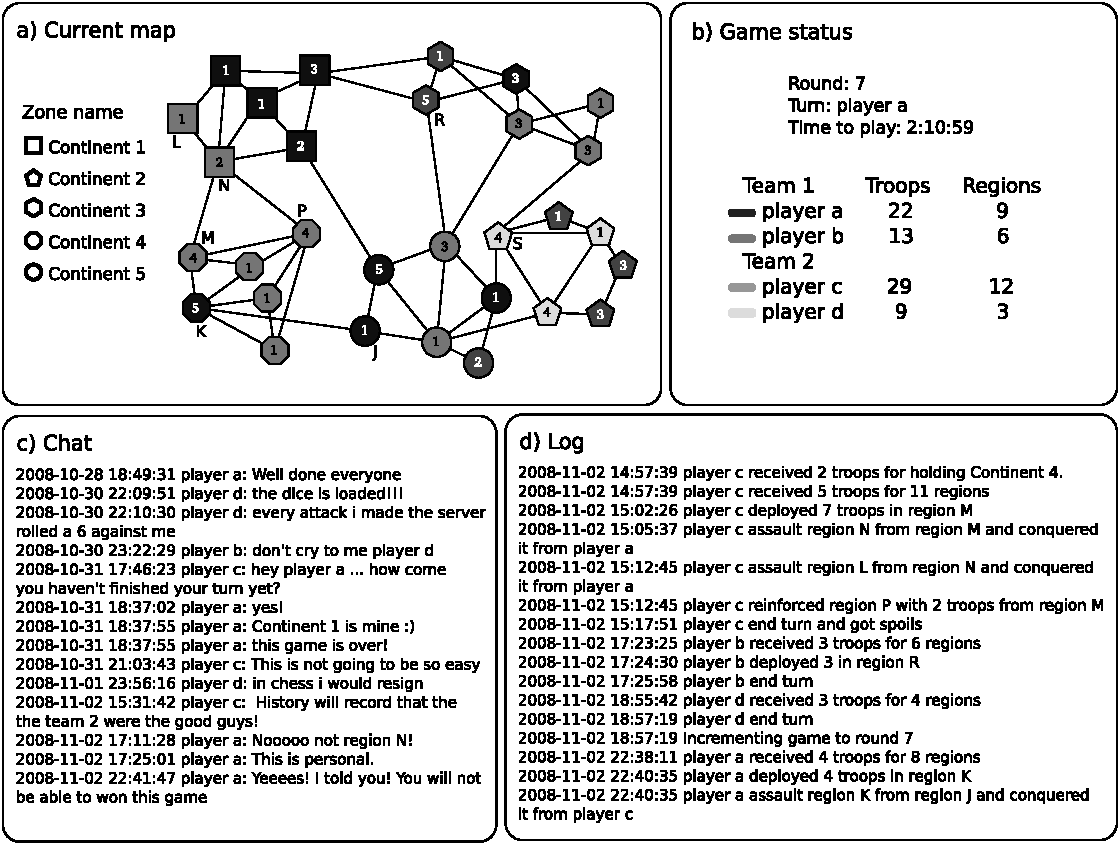
\includegraphics[width=0.8\linewidth]{figures/Fig5}
    \caption{
    Esquema del juego Conquer Club. a) El mapa mostrado como un gr\'afo con continentes (nodos con misma forma), jugadores (identificados con la escala de grises) y un n\'umero de tropas en cada regi\'on.
    b) Estado general del juego: ronda actual, jugador activo y tiempo restante para jugar; y un resumen del total de tropas y regiones controladas para cada jugador.
    c) Ejemplo de sesi\'on de chat durante un juego.
    d) Registro del juego utilizado para extraer informaci\'on a trav\'es del web scrapper.
    }
    \label{conquerImage}
\end{figure}

Cuando el jugador termina los asaltos, se pueden usar algunas tropas para reforzar la posici\'on de defensa.
%
El jugador puede mover algunas (pero no todas) las tropas de una de sus regiones a cualquier otra de sus regi\'on que est\'en conectadas.
%
La configuraci\'on de las reglas del juego de refuerzos determina cu\'antas de estas jugadas de refuerzo est\'an permitidas.
%
En nuestro ejemplo, el jugador $c$ refuerza la regi\'on $P$ moviendo dos tropas de la regi\'on $M$.
%
Finalmente, el jugador $c$ termina el turno y el jugador $b$ comienza con su ronda.

\paragraph{Matchmaking}

La plataforma tiene una secci\'on ``Unirse a un juego'', donde todos los jugadores pueden ver todos los juegos abiertos.
%
Cuando un jugador crea un juego, elige: a) opciones de juego, b) tipo de juego, todos contra todos o juego en equipo, c) el n\'umero de participantes, y d) el m\'etodo de participaci\'on, p\'ublico, p\'ublico con espacios reservados, y privado
%
Los juegos p\'ublicos son aquellos a los que cualquiera puede unirse.
%
Los juegos p\'ublicos con espacios reservados tienen espacios asignados a jugadores particulares, y el resto est\'a abierto a jugadores generales.
%
En los juegos privados solo las personas que tenga la contrase\~na pueden jugar.

% Parrafo

En esta plataforma, no existe un mecanismo de formaci\'on de equipos autom\'atico basado en la probabilidad de ganar entre jugadores.
%
Hay una clasificaci\'on interna y un sistema de puntos que los jugadores pueden usar como referencia para estimar la habilidad de los dem\'as.
%
El sistema de puntos se actualiza como {\small $\Delta = \text{min}(\frac{\text{Loser's score}}{\text{Winner's score}}20\,,\,100 )$}.
%
Sin embargo, no son indicadores precisos de la habilidad de los jugadores y la probabilidad de ganar entre oponentes.
%
El ranking interno es la conjunci\'on entre el n\'umero de partidos jugados y los puntos alcanzados.

% Parrafo

Cuando un jugador selecciona un juego, puede ver los nombres de los que ya se han unido.
%
Aparece un icono y una estrella junto a los nombres.
%
Los iconos representan el ranking de habilidad interno.
%
Las estrellas resumen la opini\'on sobre la jugadora que expresaron algunos de sus anteriores contrincantes.
%
Al final de un juego, los jugadores pueden reportar, en una escala de 1 a 5, el comportamiento del resto de jugadores en cuanto a Fair Play, Gameplay y Actitud.
%
















































































\chapter{Resultado 2. Implementaci\'on del estimador de habilidad estado del arte} \label{ch:ttt}

Si bien las redes bayesianas han mostrado ser \'utiles para evaluar el aprendizaje en los sistemas educativos, hace falta m\'as trabajo en el desarrollo de redes bayesianas din\'amicas~\cite{Almond2015}.
%
Por ejemplo, los estimadores de habilidad m\'as utilizados en la industria del video juego, como Elo y TrueSkill, no permiten obtener estimaciones iniciales fiables ni garantizar la comparabilidad entre estimaciones distantes en el tiempo y el espacio debido a que propagan la informaci\'on en una sola direcci\'on a trav\'es del sistema, utilizando el \'ultimo posterior como prior del siguiente evento.
%
Durante el doctorado descubrimos la especificaci\'on de un modelo conocido como TrueSkill Through Time (TTT), que propaga toda la informaci\'on hist\'orica a trav\'es del sistema, lo que permite realizar estimaciones fiables de la habilidad inicial y garantizar la comparabilidad hist\'orica.
%
Si bien el modelo TTT fue publicado hace m\'as una d\'ecada, no se encontraba disponible hasta entonces en ning\'un lenguajes de programaci\'on.
%
Por ello, decidimos realizar nuestra propia implementaci\'on con la que ofrecimos el primer software para \texttt{Julia}, \texttt{Python} y \texttt{R}, acompa\~nado por una explicaci\'on intuitiva comprensible para el p\'ublico general, y otra explicaci\'on en profundidad espec\'ifica para las persona con conocimientos b\'asicos en probabilidad.
%
La mejora de este modelo se hace evidente a partir de las predicciones a priori, que son varios \'ordenes de magnitud m\'as precisas que las obtenidas con los modelos mencionados.
%
Con no m\'as de tres hiperpar\'ametros intuitivos, el modelo TTT logra resultados similares y hasta mejores que modelos m\'as complejos como KickScore, de forma m\'as eficiente.
%
Luego de ilustrar su modo de uso b\'asico, mostramos c\'omo estimar la curvas de aprendizaje de los jugadores hist\'oricos de la Asociaci\'on de Tennis Profesional (ATP).
%
Este algoritmo requiere pocas iteraciones para converger, permitiendo analizar millones de observaciones usando cualquier ordenador de gama baja.

\section{Introducci\'on} \label{sec:intro}

% \en{Humans develop complex skills through time. }%
% \es{Los humanos desarrollamos habilidades complejas a trav\'es del tiempo. }%
% %
% \en{Knowing how individual abilities change is essential in a wide range of activities. }%
% \es{Saber c\'omo cambian las capacidades individuales es esencial en varias actividades. }%
% %

Todos los estimadores de habilidad ampliamente utilizados en la actualidad comparten alguna variante del modelo causal propuesto por Elo~\cite{Glickman1999, Herbrich2007, VanDerLinden2016}.
%
La figura~\ref{fig:generative_model} ofrece un modelo causal en el que las habilidades generan el resultado observable.
%
\begin{figure}[ht!]
\centering \small
    \tikz{
    \node[det, fill=black!10] (r) {$r$} ;
    \node[const, left=of r, xshift=-1.35cm] (r_name) {\small Resultado:};
    \node[const, right=of r] (dr) {\normalsize $ r = (d > 0)$};
    \node[latent, above=of r, yshift=-0.45cm] (d) {$d$} ; %
    \node[const, right=of d] (dd) {\normalsize $ d = p_i-p_j$};
    \node[const, left=of d, xshift=-1.35cm] (d_name) {\small Diferencia:};
    \node[latent, above=of d, xshift=-0.8cm, yshift=-0.45cm] (p1) {$p_i$} ; %
    \node[latent, above=of d, xshift=0.8cm, yshift=-0.45cm] (p2) {$p_j$} ; %
    \node[const, left=of p1, xshift=-0.55cm] (p_name) {\small Desempe\~no:};
    \node[accion, above=of p1,yshift=0.3cm] (s1) {} ; %
    \node[const, right=of s1] (ds1) {$s_i$};
    \node[accion, above=of p2,yshift=0.3cm] (s2) {} ; %
    \node[const, right=of s2] (ds2) {$s_j$};
    \node[const, right=of p2] (dp2) {\normalsize $p \sim \N(s,\beta^2)$};
    \node[const, left=of s1, xshift=-.85cm] (s_name) {\small Habilidad:};
    \edge {d} {r};
    \edge {p1,p2} {d};
    \edge {s1} {p1};
    \edge {s2} {p2};
}
     \caption{
    Modelo generativo en el que las habilidades causan los resultados observables a trav\'es de la diferencia de rendimientos ocultos, $d=p_i-p_j$, ambas variables aleatorias centradas en la verdadera habilidad, $p \sim \N(s,\beta^2)$.
    %
    Quien haya obtenido mayor rendimiento gana, $r = (d > 0)$.
    %
    Las variables observables se pintan de gris, las ocultas en blanco, y las constantes se muestran como puntos negros.
    }
    \label{fig:generative_model}
\end{figure}
%
Los agentes exhiben distintos desempe\~nos en cada evento, que var\'ian alrededor de su verdadera habilidad, $\N(p\,|\,s,\beta^2)$.
%
El modelo supone que gana el agente con mayor rendimiento, $r = (p_i > p_j)$.
%
El par\'ametro $\beta^2$, al ser el mismo para todos los agentes, act\'ua como la escala de las estimaciones: habilidades a una distancia de un $\beta$ implica 76\% probabilidad de ganar, independiente del valor absoluto de las estimaciones%

% Parrafo

Los estimadores de habilidad com\'unmente utilizados en la industria del video juego y la academia, como Elo, Glicko~\cite{Glickman1999}, TrueSkill \cite{Herbrich2007} e IRT \cite{Fox2010,VanDerLinden2016}, no pueden obtener estimaciones iniciales fiables ni asegurar la comparabilidad hist\'orica debido a que propagan la informaci\'on en una sola direcci\'on a trav\'es del sistema, utilizando el \'ultimo posterior como prior del siguiente evento (enfoque \emph{filtering}).

%

El enfoque adoptado por TrueSkill para tratar el proceso din\'amico, conocido como \emph{filtering}, usa el \'ultimo posterior aproximado como prior del siguiente evento.
%
Luego, el posterior aproximado en un determinado momento se define como,
%
\begin{equation}\label{eq:filter} %\tag{\text{filtering}}
 \widehat{\text{Posterior}}_t \propto \widehat{\text{Likelihood}}_t  \overbrace{\widehat{\text{Likelihood}}_{t-1} \dots \underbrace{\widehat{\text{Likelihood}}_{1} \text{Prior}_1}_{\widehat{\text{Posterior}}_{1} \text{ como } \text{Prior}_{2}} }^{\widehat{\text{Posterior}}_{t-1} \text{ \en{as}\es{como} } \text{Prior}_{t}} %= \text{Prior}_1 \prod_{i=1}^t \text{Likelihood}_i
\end{equation}
%
Donde {\footnotesize $\widehat{\text{Posterior}}_i$} y {\footnotesize $\widehat{\text{Likelihood}}_i$} representan la aproximaciones inducidas por la ecuaci\'on~\eqref{eq:approx} en el $i$-\'esimo evento.
%
Si consideramos la verosimilitud como un filtro del prior, cada posterior puede ser visto como una acumulaci\'on de todos los filtros anteriores.
%
De esta forma, la informaci\'on propaga del estimaciones pasadas hacia futuras.
%
Debido a que las habilidades cambian en el tiempo, es importante agregar alguna incertidumbre $\gamma$ luego de cada paso.
%
\begin{equation}\label{eq:dynamic_factor}
 \widehat{p}(s_{i_t}) = \N(s_{i_t} | \mu_{i_{t-1}}, \sigma_{i_{t-1}}^2 + \gamma^2 )
 \end{equation}
 %
Debido a que el enfoque de filtrado es un procedimiento ad-hoc que no surge de ning\'un modelo probabil\'istico, sus estimaciones exhiben una serie problemas.
%
El m\'as obvio es que el inicio de toda secuencia de estimaciones siempre tiene alta incertidumbre.
%
Pero tambi\'en pueden producirse desacoplamientos temporales y espaciales que impidan comparar estimaciones distantes.
%
Aunque la diferencias relativas entre estimaciones contempor\'aneas al interior de comunidades bien conectadas sean correctas, las estimaciones separadas en el tiempo y entre comunidades poco conectadas pueden ser incorrectas.
%
Todos estos problemas est\'an relacionados al hecho de que la informaci\'on propaga en una sola direcci\'on a trav\'es del sistema, cuando la inferencia deber\'ia realizarse con toda la informaci\'on disponible, tambi\'en de eventos que ocurren de forma paralela como de eventos futuros disponibles.

\subsection{TrueSkill Through Time model}

Para corregir los problemas del algoritmo TrueSkill es necesario realizar la inferencia dentro de una red bayesiana que inlcuya todas las actividades hist\'oricas, de modo que la informaci\'on pueda propagar por todo el sistema.
%
De esta forma se garantiza tanto buenas estimaciones iniciales como la comparabilidad de las estimaciones que est\'an separadas en el tiempo y el espacio.
%
La conectividad entre eventos surge de suponer que la habilidad de un jugador en un tiempo $t$ depende de su propia habilidad en un tiempo anterior $t-1$, generando un red que adquiere su estructura dependiendo de quienes participan en cada evento.
%
Algoritmos similares fueron implementados por \cite{Coulom2008} y \cite{Maystre2019} basados en aproximaciones laplacianas y procesos gaussianos respectivamente.
%
Exluyendo el aspecto din\'amico, $\gamma = 0$, el prior de un agente $i$ en el $t$-\'esimo evento es el producto del todas sus verosimilitudes, salvo la del $t$-\'esimo evento.
%
\begin{equation}\label{eq:smooth_prior}
 \text{Prior}_{i_t} = \text{Prior}_{i_0} \underbrace{\prod_{k = 1}^{t-1} \text{Verosimilitud}_{i_k}}_{\text{\en{Past information}\es{Informaci\'on pasada}}} \underbrace{\prod_{k = t + 1}^{T_i} \text{\en{Likelihood}\es{Verosimilitud}}_{i_k}}_{\text{\en{Future information}\es{Informaci\'on futura}}}
\end{equation}
%
Donde $T_i$ es la cantidad total de eventos del agente $i$, siendo {\small Prior$_{i_0}$} su prior inicial.
%
Esto produce una mutua dependencia entre estimaciones que nos obliga a usar iterativamente las \'ultimas verosimilitudes disponibles hasta alcanzar convergencia (detalles en la secci\'on~\ref{sec:throughTime}).
%
\begin{figure}[ht!]
  \centering
  \scalebox{.9}{
    \tikz{ %
      \node[latent] (s10) {$s_{a_0}$} ;
      %
      \node[latent,  below=of s10,yshift=-0.7cm] (s11) {$s_{a_1}$} ;
      \node[latent, right=of s11, xshift=3cm] (p11) {$p_{a_1}$} ;
      %
      \node[latent, below=of s11,yshift=-0.4cm] (s12) {$s_{a_2}$} ;
      \node[latent, right=of s12, xshift=3cm] (p12) {$p_{a_2}$} ;
      \node[const, right=of p11,xshift=0.5cm] (r1) {$\bm{>}$} ;
      \node[const, above=of r1, yshift=0.3cm] (nr1) {\footnotesize \ \  Observed result} ;
      \node[const, right=of p12,xshift=0.5cm] (r2) {$\bm{<}$} ;
      \node[const, above=of r2, yshift=0.3cm] (nr2) {\footnotesize \ \ Observed result} ;
      \node[latent, left=of s10, xshift=13.4cm] (s20) {$s_{b_0}$} ;
      \node[latent, below=of s20,yshift=-0.7cm] (s21) {$s_{b_1}$} ;
      \node[latent, left=of s21, xshift=-3cm] (p21) {$p_{b_1}$} ;
      \node[latent, below=of s21, yshift=-0.4cm] (s22) {$s_{b_2}$} ;
      \node[latent, left=of s22, xshift=-3cm] (p22) {$p_{b_2}$} ;
      \edge {s10} {s11};
      \edge {s11} {s12};
      \edge {s20} {s21};
      \edge {s21} {s22};
      \edge {s11} {p11};
      \edge {s12} {p12};
      \edge {s21} {p21};
      \edge {s22} {p22};
      \node[const, right=of s10, yshift=0cm ] (wp10) {\includegraphics[page={13},width=.125\linewidth]{figures/smoothing}} ;
      \node[const, left=of s20, yshift=0cm ] (wp20) {\includegraphics[page={13},width=.125\linewidth]{figures/smoothing}} ;
      \node[const, left=of s11, yshift=0.6cm ] (post11) {\includegraphics[page={1},width=.125\linewidth]{figures/smoothing}} ;
      \node[const, right=of s11, yshift=0.6cm ] (wp11) {\includegraphics[page={2},width=.125\linewidth]{figures/smoothing}} ;
      \node[const, left=of p11, yshift=0.6cm ] (lh11) {\includegraphics[page={3},width=.125\linewidth]{figures/smoothing}} ;
      \node[const, left=of s12, yshift=0.6cm ] (post12) {\includegraphics[page={4},width=.125\linewidth]{figures/smoothing}} ;
      \node[const, right=of s12, yshift=0.6cm ] (wp12) {\includegraphics[page={5},width=.125\linewidth]{figures/smoothing}} ;
      \node[const, left=of p12, yshift=0.6cm ] (lh12) {\includegraphics[page={6},width=.125\linewidth]{figures/smoothing}} ;
      \node[const, right=of s21, yshift=0.6cm ] (post21) {\includegraphics[page={7},width=.125\linewidth]{figures/smoothing}} ;
      \node[const, left=of s21, yshift=0.6cm ] (wp21) {\includegraphics[page={8},width=.125\linewidth]{figures/smoothing}} ;
      \node[const, right=of p21, yshift=0.6cm ] (lh21) {\includegraphics[page={9},width=.125\linewidth]{figures/smoothing}} ;
      \node[const, right=of s22, yshift=0.6cm ] (post22) {\includegraphics[page={10},width=.125\linewidth]{figures/smoothing}} ;
      \node[const, left=of s22, yshift=0.6cm ] (wp22) {\includegraphics[page={11},width=.125\linewidth]{figures/smoothing}} ;
      \node[const, right=of p22, yshift=0.6cm ] (lh22) {\includegraphics[page={12},width=.125\linewidth]{figures/smoothing}} ;
      \node[const, above=of post11] (npost11) {\scriptsize Posterior} ;
      \node[const, above=of wp11] (nwp11) {\scriptsize Prior} ;
      \node[const, above=of lh11] (nlh11) {\scriptsize Verosimilitud} ;
      \node[const, above=of post21] (npost21) {\scriptsize Posterior} ;
      \node[const, above=of wp21] (nwp21) {\scriptsize Prior} ;
      \node[const, above=of lh21] (nlh21) {\scriptsize Verosimilitud} ;
      \node[const, above=of post12] (npost12) {\scriptsize Posterior} ;
      \node[const, above=of wp12] (nwp12) {\scriptsize Prior} ;
      \node[const, above=of lh12] (nlh12) {\scriptsize Verosimilitud} ;
      \node[const, above=of post22] (npost22) {\scriptsize Posterior} ;
      \node[const, above=of wp22] (nwp22) {\scriptsize Prior} ;
      \node[const, above=of lh22] (nlh22) {\scriptsize Verosimilitud} ;
      \node[const, above=of wp10,yshift=-0.55cm] (nwp10) {\scriptsize Prior} ;
      \node[const, above=of wp20,yshift=-0.55cm] (nwp20) {\scriptsize Prior} ;
      }
  }
  \caption{
  Convergencia de una red Bayesiana con dos eventos y dos agentes: la primera partida la gana el jugador $a$ y la segunda la gana el jugador $b$.
  %
  La luminosidad de las curvas indican el orden: la primera (la m\'as clara) correponde a las estimaciones de TrueSkill, y la \'ultima (la m\'as oscura) correponde con las estimaciones de TrueSkill Through Time.
  }
  \label{fig:smooth_example}
\end{figure}
%
En la figura~\ref{fig:smooth_example} mostramos c\'omo convergen las estimaciones en una red bayesiana dos agentes y dos eventos.
%
TrueSkill Through Time recupera, de acuerdo a lo que sugieren los datos (una victoria cada uno), las verdaderas diferencias entre habilidades indicando que ambos jugadores tienen misma habilidad (posterior centrado en cero), a diferencia de TrueSkill que ofrece estimaciones sesgadas.
% Parrafo

La ventaja de TrueSkill Through Time radica en que el modelo causal temporal permite que la informaci\'on propage correctamente por todo el sistema.
%
A diferencia de las redes neuronales que tienen estructuras regulares, estas redes bayesianas adquieren siempre una estructura compleja, creci\'endo t\'ipicamente a millones de par\'ametros (e.g., videojuego).
%
El procedimiento converge con unas pocas iteraciones lineales sobre los datos.
%
La correcci\'on de los sesgos es un paso fundamental para construir estimadores confiables que sirvan tanto para la toma de decisiones en \'areas sensibles como para la evaluaci\'on de teor\'ias cient\'ificas que utilicen la habilidad como dato observable.
%
Con este art\'iculo ponemos a disposici\'on los primeros paquetes de TrueSkill Through Time para \texttt{Julia}, \texttt{Python} y \texttt{R}, junto con su documentaci\'on cient\'ifica completa~\cite{Landfried-repo:ttt}.


\subsection{Evaluaci\'on de modelos}

El modelo TrueSkill Through Time (TTT)~\cite{Dangauthier2007} propaga la informaci\'on hist\'orica a trav\'es de toda la red, proporcionando estimaciones con baja incertidumbre en cualquier momento, ofreciendo estimaciones iniciales de habilidad fiables y garantizando la comparabilidad de las estimaciones distantes en el tiempo y el espacio (enfoque \emph{smoothing}).
%
Enfoque similares fueron implementados por \cite{Coulom2008} (Whole History Rating) y \cite{Maystre2019} (KickScore), basados en aproximaciones laplacianas y procesos gaussianos respectivamente.
% Parrafo

En la tabla~\ref{Tab:Models} comparamos nuestra implementaci\'on del algoritmo TTT contra KickScore TrueSkill, Elo, y un modelo ``Constante'' en el que las habilidades no cambian en el tiempo.
%
Para evaluar los modelos debemos calcular su probabilidad dados los datos,%
%
\begin{equation}
 P(\text{Modelo}|\text{Datos}) = \frac{P(\text{Dat\en{a}\es{os}}|\text{Model\es{o}})P(\text{Model\es{o}})}{P(\text{Dat\en{a}\es{os}})}
\end{equation}
%
Cuando no tenemos acceso a todos los modelos, no podremos calcular la probabilidad $P(\text{Modelo}|\text{Datos})$, pero s\'i podremos comparar modelos.
%
\begin{equation}\label{eq:bayes_factor}
 \frac{P(\text{Modelo}_i|\text{Dat\en{a}\es{os}})}{P(\text{Model\es{o}}_j|\text{Dat\en{a}\es{os}})} = \frac{P(\text{Dat\en{a}\es{os}}|\text{Model\es{o}}_i)P(\text{Model\es{o}}_i)}{P(\text{Dat\en{a}\es{os}}|\text{Model\es{o}}_j)P(\text{Model\es{o}}_j)} \overset{\text{\en{if}\es{si} } *}{=} \frac{P(\text{Dat\en{a}\es{os}}|\text{Model\es{o}}_i)}{P(\text{Dat\en{a}\es{os}}|\text{Model\es{o}}_j)}
\end{equation}
%
Esta expresi\'on se conoce como el \emph{Bayes factor}, el cual se suele expresar en escala logar\'itmica para reportar la diferencia en \'ordenes de magnitud.
%
En el caso especial en el que no tenemos preferencia a priori sobre ning\'un modelo (
%
\begin{equation}
P(\text{Dat\en{a}os}|\text{Model\es{o}}) = P(d_1|\text{Model\es{o}})P(d_2|d_1,\text{Model\es{o}}) \dots P(d_n|d_1,\dots, d_{n-1},\text{Model\es{o}})
\end{equation}
%
donde cada elementos de la productoria es una predicci\'on del siguiente dato en base a los datos previos y el modelo.
%
En este trabajo tambi\'en vamos a reportare la media geom\'etrica debido a que puede interpretarse como la predicci\'on ``caracter\'istica'' del modelo,%
%
\begin{equation}\label{eq:gmean}
P(\text{Dat\en{a}os}|\text{Model\es{o}}) = \text{geometric mean}(P(\text{Dat\en{a}\es{os}}|\text{Model\es{o}}))^{|\text{Dat\en{a}\es{os}}|}
\end{equation}
%
donde $|\text{Datos}|$ representa el tama\~no del conjunto de datos.
% Parrafo

Para realizar la comparaci\'on seguiremos la metodolog\'ia empleada por \cite{Maystre2019} analizando las cuatro base de datos sobre las cuales ellos reportan sus predicciones a priori: ATP (tenis), NBA (baloncesto), FIFA (f\'utbol), y FIDE (ajedrez).
Usamos el \SI{70}{\percent} inicial de la base de datos para entrenar los hiperpar\'ametros y el \SI{30}{\percent} final para evaluar los modelos.
%
Para predecir el resultado de una observaci\'on en el tiempo $t$, ellos utilizan todos los datos (en los conjuntos de entrenamiento y de prueba) hasta el d\'ia anterior a $t$.
%
La tabla~\ref{Tab:Models} se resumen las comparaciones de los modelos en las cuatro base de datos.
%
\begin{table}[ht!] \centering
  \scriptsize
  \begin{tabular}{c|cc|cc|cc|cc|c||c}
 \multirow{2}{*}{$\hfrac{\text{\scriptsize Dataset}}{\text{Test size}}$} & \multicolumn{2}{c|}{Constante$^\dagger$}& \multicolumn{2}{c|}{Elo$^\dagger$} & \multicolumn{2}{c|}{TrueSkill} & \multicolumn{2}{c|}{KickScore$^\dagger$} &  \multicolumn{2}{c}{TTT} \\
 & GM & $\log_2$BF & GM & $\log_2$BF & GM & $\log_2$BF & GM & $\log_2$BF & GM & LOOCV \\ \hline
\multirow{2}{*}{$\hfrac{\text{\scriptsize Ten\en{n}is}}{\num{186361}}$} & \multirow{2}{*}{$0.5593$} & \multirow{2}{*}{\num{7910}} & \multirow{2}{*}{$0.5695$} & \multirow{2}{*}{\num{3051}} & \multirow{2}{*}{$0.5722$} & \multirow{2}{*}{\num{1780}} & \multirow{2}{*}{$0.5758$} & \multirow{2}{*}{\num{93}} & \multirow{2}{*}{$\bm{0.5760}$} & \multirow{2}{*}{${0.5908}$} \\
 & & & & & & & & & & \\
 \multirow{2}{*}{$\hfrac{\text{\scriptsize Basketball}}{\num{20300}}$} & \multirow{2}{*}{$0.5006$} & \multirow{2}{*}{\num{1771}} & \multirow{2}{*}{$0.5305$} & \multirow{2}{*}{\num{72}} & \multirow{2}{*}{$0.5316$} & \multirow{2}{*}{\num{11}} & \multirow{2}{*}{$\bm{0.5328}$} & \multirow{2}{*}{-55} & \multirow{2}{*}{${0.5318}$} & \multirow{2}{*}{${0.5382}$} \\
  & & & & & & & & & & \\
 \multirow{2}{*}{$\hfrac{\text{\scriptsize Chess}}{\num{92004}}$} & \multirow{2}{*}{$0.3570$} & \multirow{2}{*}{\num{520}} & \multirow{2}{*}{$0.3552$} & \multirow{2}{*}{\num{1190}} & \multirow{2}{*}{$0.3580$} & \multirow{2}{*}{\num{148}} & \multirow{2}{*}{$\bm{0.3584}$} & \multirow{2}{*}{0} & \multirow{2}{*}{$\bm{0.3584}$} & \multirow{2}{*}{${0.3641}$} \\
 & & & & & & & & & \\
 \multirow{2}{*}{$\hfrac{\text{\scriptsize \en{Football}F\'utbol}}{\num{5759}}$} & \multirow{2}{*}{$0.3949$} & \multirow{2}{*}{\num{30}} & \multirow{2}{*}{$0.3867$} & \multirow{2}{*}{\num{204}} & \multirow{2}{*}{$0.3921$} & \multirow{2}{*}{\num{89}} & \multirow{2}{*}{$\bm{0.3961}$} & \multirow{2}{*}{\num{4}} & \multirow{2}{*}{$\bm{0.3963}$} &  \multirow{2}{*}{${0.3974}$} \\
  & & & & & & & & & & \\ \hline
  \end{tabular}
  \caption{
  Comparaciones de modelos en cuatro base de datos.
  %
  Las columnas GM reportan la media geom\'etrica de las predicciones a priori de los modelos (ecuaci\'on \ref{eq:gmean}).
  %
  Las columnas $\text{log}_2$BF reportan el Bayes Factor (ecuaci\'on \ref{eq:bayes_factor}) entre TTT y otros modelos en escala logar\'itmica.
  %
  Como referencia, la columna LOOCV reporta la media geom\'etrica de las predicciones usando toda la informaci\'on hist\'orica, $p(d_i| d_1, \dots, d_{i-1}, d_{i+1}, \dots, d_n , M)$.
  %
  La media geom\'etrica de los modelos se\~nalados con el s\'imbolo $\dagger$ fue obtenida por \cite{Maystre2019}.
  }
  \label{Tab:Models}
\end{table}
%
El modelo TTT supera KickScore en la base de datos de tenis por $93$ \'ordenes de magnitud, mientras que KickScore supera a TTT en la base de ajedrez por $55$ \'ordenes de magnitud.
%
Consideramos que los modelos empatan en las bases de datos de ajedrez y de f\'utbol en tanto la diferencia entre s es menor a 10 \'ordenes de magnitud.
%
Unificando las cuatro base de datos en una sola, el modelo TTT supera a KickScore por m\'as de 40 \'ordenes de magnitud.
% Parrafo

Para computar las predicciones ellos utilizan un cluster para crear en paralelo un modelo diferente por cada d\'ia $t$, que requieren cada uno cerca de 100 iteraciones para alcanzar convergencia.
%
En cambio, para nosotros fue suficiente usar una computadora de escritorio para crear un \'unico modelo al que le agregamos las datos d\'ia a d\'ia, realizando una \'unica iteraci\'on en cada paso.
%
La selecci\'on de modelo la hemos realizado optimizando los hiperpar\'ametros, pero una selecci\'on de modelo bayesiana completa deber\'ia computar las predicciones integrando todo el espacio de hiperpar\'ametros.
%
Este procedimiento suele penalizar a los modelos complejos cuando la b\'usqueda en el espacio de hiperpar\'ametros es innecesaria.
%
Con no m\'as de tres hiperpar\'ametros intuitivos (incertidumbre a priori, incertidumbre din\'amica y probabilidad de empate), el modelo TTT logra resultados similares y hasta mejores que KickScore de forma m\'as eficiente, debido a que el \'ultimo debe optimizar en un espacio de par\'ametros mucho m\'as grande, que incluye la definci\'on de un \emph{kernel} y luego los hiperpar\'ametros espec\'ificos a ese \emph{kernel}.
% Parrafo

Cuando el objetivo es estimar las curvas de aprendizaje en el tiempo con la mayor precisi\'on posible, en vez de forzar al modelo a hacer la inferencia usando solamente la informaci\'on del pasado (como hicimos para comparar el desempe\~no de los modelos), conviene hacer la inferencia usando toda la informaci\'on hist\'orica.
%
Esto es \'util debido a que los modelos probabil\'isiticos pueden usar informaci\'on del futuro para inferir eventos del pasado, algo que intuitivamente hacemos cuando sospechamos que los deportistas destacados tambi\'en eran h\'abiles un tiempo antes de hacerse conocidos.
%
La columna LOOCV de la tabla~\ref{Tab:Models} reporta la media geom\'etrica de las predicciones que usan toda la informaci\'on hist\'orica excepto el evento que se est\'a prediciendo, $p(d_i| d_1, \dots, d_{i-1}, d_{i+1}, \dots, d_n , M)$.
%
Si bien no usamos estas predicciones offline para comparar modelos (Bayes Factor), es interesante notar que incorporar toda la informaci\'on hist\'orica al modelo TTT mejora sus propias estimaciones centenas de \'ordenes de magnitud.
% Parrafo

Debido a que la estimaci\'on de habilidad es un problema sensible para los individuos, en las siguientes secciones ofrecemos una explicaci\'on lo m\'as intuitiva y completa posible.
%
Las comunidades que son evaluadas tanto en la industria del video juego como en los sistemas educativos necesitan conocer c\'omo funciona el algoritmo que mide su habilidad.
%
Este trabajo, adem\'as de ofrecer una herramienta de software, ofrece una reporte cient\'ifico completo y accesible al p\'ublico en general.




\section{Software: implementaci\'on del modelo}


En esta secci\'on ofrecemos la documentaci\'on matem\'atica completa del modelo TrueSkill Through Time.
%
La ventaja de este modelo reside en la aplicaci\'on estricta de la teor\'ia de la probabilidad: todos los supuestos se hacen expl\'icitos a trav\'es de un modelo generativo, y la inferencia se resuelve s\'olo con las regla de la probabilidad, nada m\'as que las reglas de la suma y el producto.
%
En la secci\'on~\ref{sec:sumProductAlgorithm} introducimos el \emph{sum-product algorithm}, que nos permite aplicar eficientemente estas reglas para computar las distribuciones marginales, e.g., el posterior y la predicci\'on a priori.
%
En la secci\'on~\ref{sec:propiedades} enumeramos las propiedades que necesitaremos para derivar las distribuciones marginales de inter\'es.
%
En las secci\'on \ref{sec:Gaussian} introducimos las operaciones de la clases \texttt{Gaussian}, la que realiza la mayor parte del c\'omputo.
%
En las secciones \ref{sec:2vs2}, \ref{sec:empate}, \ref{sec:approximate_posterior}, mostramos c\'omo resolver la predicci\'on a priori y el posterior exacto de un evento, incorporamos empate al modelo y explicamos c\'omo aproximar el posterior exacto en partidas con dos equipos.
%
En la secci\'on \ref{sec:iterative_posterior} explicamos la soluci\'on general multi-equipos, que requiere la aplicaci\'on de un algoritmo iterativo.
%
En la secci\'on~\ref{sec:throughTime} justificamos los pasos matem\'aticos requeridos para resolver el modelo TrueSkill Through Time completo.


\subsection{Sum-product algorithm} \label{sec:sumProductAlgorithm}

El \emph{sum-product algorithm}~\cite{Kschischang2001} aprovecha la estructura de la distribuci\'on de probabilidad conjunta, impuesta por el modelo causal, para aplicar eficientemente las reglas de la probabilidad.
%
Cualquier modelo puede factorizarse en el producto de probabilidades condicionales.
%
Haciendo uso de las independencias entre las variables, nuestro modelo (figura~\ref{fig:generative_model}) puede factorizarse como,
%
\begin{equation} \label{eq:factorization}
 p(\bm{s},\bm{p},d,r) = p(s_1)p(s_2)p(p_1|s_1)p(p_2|s_2)p(d|\bm{p})P(r|d)
\end{equation}
%
En la figura~\ref{fig:factor_graph} mostramos esta factorizaci\'on graficamente.
%
Este tipo de representaciones, conocidas como \emph{factor graph}, son gr\'afos con dos tipos de nodos: nodos variables (c\'irculos blancos), y nodos funciones (cuadrados negros).
%
Los ejes entre nodos variables y nodos funciones representan la relaci\'on matem\'atica ``la variable $v$ es argumento de la funci\'on $f$''.
%
\begin{figure}[ht!]
\centering \small
    \tikz{
%         \node[const, above=of fr] (nfr) {$f_r$}; %
% 	\node[const, above=of nfr] (dfr) {\large $\mathbb{I}(d >0)$}; %
    \node[factor] (fr) {} ;
    \node[const, left=of fr] (nfr) {\normalsize $P(r|d)$};
    \node[const, right=of fr] (dfr) {\normalsize \hspace{2.4cm} $P(r|d)=\mathbb{I}(d>0)$};
    \node[latent, above=of fr, yshift=-0.6cm] (d) {$d$} ; %
    \node[const, left=of d, xshift=-1.35cm] (d_name) {\small Diferencia:};
    \node[factor, above=of d,yshift=-0.6cm] (fd) {} ;
    \node[const, left=of fd] (nfd) {\normalsize $p(d|\bm{p})$};
    \node[const, right=of fd] (dfd) {\normalsize \hspace{2.4cm} $p(d|\bm{p}) =\delta(d=p_1-p_2) $};
    \node[latent, above=of fd, xshift=-0.8cm, yshift=-0.6cm] (p1) {$p_1$} ; %
    \node[latent, above=of fd, xshift=0.8cm, yshift=-0.6cm] (p2) {$p_2$} ; %
    \node[const, left=of p1, xshift=-0.55cm] (p_name) {\small Rendimiento:};
    \node[factor, above=of p1 ,yshift=-0.6cm] (fp1) {} ;
    \node[factor, above=of p2 ,yshift=-0.6cm] (fp2) {} ;
    \node[latent, above=of fp1,yshift=-0.6cm] (s1) {$s_1$} ; %
    \node[latent, above=of fp2,yshift=-0.6cm] (s2) {$s_2$} ; %
    \node[factor, above=of s1 ,yshift=-0.6cm] (fs1) {} ;
    \node[factor, above=of s2 ,yshift=-0.6cm] (fs2) {} ;
    \node[const, left=of fp1] (nfp1) {\normalsize $p(p_1|s_1)$};
    \node[const, right=of fp2] (nfp2) {\normalsize $p(p_2|s_2)$};
    \node[const, right=of fp2] (dfp2) {\normalsize \hspace{1.6cm} $p(p_i|s_i)=\N(p_i|s_i,\beta^2)$};
    \node[const, left=of s1, xshift=-.85cm] (s_name) {\small Habilidad:};
    \node[const, left=of fs1] (nfs1) {\normalsize $p(s_1)$};
    \node[const, right=of fs2] (nfs2) {\normalsize $p(s_2)$};
    \node[const, right=of fs2] (dfs) {\normalsize \hspace{1.6cm} $p(s_i) = \N(s_i|\mu_i,\sigma_i^2)$};
    \edge[-] {d} {fr};
    \edge[-] {p1,p2,d} {fd};
    \edge[-] {fp1} {p1,s1};
    \edge[-] {fp2} {p2,s2};
    \edge[-] {fs1} {s1};
    \edge[-] {fs2} {s2};
}
     \caption{%
     Forma gr\'afica de representar la factorizaci\'on de la distribuci\'on conjunta inducida por el modelo causal b\'asico (ecuaci\'on~\eqref{eq:factorization}).
     %
     Los cuadrados negros representan las funciones, los c\'irculos blancos representan las variable, y los ejes entre ellos representan la relaci\'on matem\'atica ``la variable es argumento de la funci\'on''.
     %
     }
    \label{fig:factor_graph}
\label{modelo}
\end{figure}
%
En nuestro caso querermos computar dos marginales, el posterior proporcional de las habilidades $p(s_i, r)$ y la probabilidad a priori del resultado $p(r)$.
%
El \emph{sum-product algorithm} es una forma general de descomponer las reglas de la probabilidad como mensajes que se env\'ian los nodos del \emph{factor graph}.
%
Hay dos tipos de mensajes: los mensajes que envian los nodos variables a sus funciones vecinas ($m_{v \rightarrow f}(v)$); y los mensajes que env\'ian los nodos funciones a sus variables vecinas ($m_{f \rightarrow v}(v)$).
%
El primero codifica una porci\'on de la regla del producto.
%
\begin{equation*}\label{eq:m_v_f} \tag{\text{paso del producto}}
m_{v \rightarrow f}(v) = \prod_{h \in n(v) \setminus \{f\} } m_{h \rightarrow v}(v)
\end{equation*}
%
donde $n(v)$ representa el conjunto de vecinos del nodo $v$.
%
En pocas palabras, los mensajes que env\'ia una variable $v$ es simplemente la multiplicaci\'on de los mensajes que recibi\'o del resto de sus vecinos $h \in n(v)$ salvo $f$.
%
Los mensajes que env\'ian los nodos funciones codifican una parte de la regla de la suma.
%
\begin{equation*}\label{eq:m_f_v}  \tag{\text{paso de la suma}}
m_{f \rightarrow v}(v) = \int \cdots \int \Big( f(\bm{h},v) \prod_{h \in n(f) \setminus \{v\} } m_{h \rightarrow f}(h) \Big) \,  d\bm{h}
\end{equation*}
%
donde $\bm{h} = n(f)\setminus \{v\}$ es el conjunto de todos los vecinos de $f$ salvo $v$, y $f(\bm{h},v)$ representa la funci\'on $f$, evaluada en todos sus argumentos.
%
En pocas palabras, los mensajes que env\'ia una funci\'on $f$ tambi\'en es la multiplicaci\'on de los mensajes que recibi\'o del resto de sus vecinos $h \in n(f)$ salvo $v$, por s\'i misma $f(\cdot)$, integrando (o sumando) sobre $\bm{h}$.
%
Finalmente, la distribuci\'on de probabilidad marginal de una variable $v$ es simplemente la multiplicaci\'on de los mensajes que $v$ recibe de todos sus vecinos.
%
\begin{equation*}\label{eq:marginal}  \tag{\text{probabilidad marginal}}
p(v) = \prod_{h \in n(v)} m_{h \rightarrow v}
\end{equation*}
%
Este algoritmo codifica la m\'inima cantidad de pasos que se requieren para calcular cualquier distribuci\'on de probabilidad marginal.

\subsection{Propiedades matem\'aticas y notaci\'on}\label{sec:propiedades}

La eficiencia de TrueSkill Through Time se obtiene gracias que las marginales se pueden computar de forma anal\'itica.
%
En esta secci\'on enumeramos las propiedades que necesitamos para derivar los mensajes exactos y aproximados que surgen del \emph{sum-product algorithm}.
%
La primera propiedad establece que el producto de dos distribuciones gaussianas, ambas evaluadas en el mismo punto $x$, pueden expresarse como la producto de otras dos distribuciones gaussianas con s\'olo una de ellas evaluada en $x$.
%
\begin{equation*}\label{eq:gaussian_product} \tag{\text{Producto de gaussianas}}
\N(x|\mu_1,\sigma_1^2)\N(x|\mu_2,\sigma_2^2) \overset{\ref{multiplicacion_normales}}{=} \N(\mu_1|\mu_2,\sigma_1^2+\sigma_2^2) \N(x|\mu_{*},\sigma_{*}^2)
\end{equation*}
%
con $\mu_{*} = \frac{\mu_1}{\sigma_1^2} + \frac{\mu_2}{\sigma_2^2}$ y $\sigma_{*}^2 = \left(\frac{1}{\sigma_1^2} + \frac{1}{\sigma_2^2} \right)^{-1}$.
%
Algo similar ocurre con la divisi\'on de dos distribuciones gaussianas, ambas evaluadas en el mismo punto $x$.
\begin{equation*}\label{eq:gaussian_division} \tag{\text{Divisi\'on de gaussianas}}
\N(x|\mu_1,\sigma_1^2)/\N(x|\mu_2,\sigma_2^2) \overset{\ref{sec:division_normales}}{\propto} \N(x|\mu_{\div},\sigma_{\div}^2)/\N(\mu_1|\mu_2,\sigma_1^2+\sigma_2^2)
\end{equation*}
%
con $\mu_{\div} = \frac{\mu_1}{\sigma_1^2} - \frac{\mu_2}{\sigma_2^2}$ y $\sigma_{\div}^2 = \left(\frac{1}{\sigma_1^2} - \frac{1}{\sigma_2^2} \right)^{-1}$.
La funci\'on indicadora $\mathbb{I}(\cdot=\cdot)$ vale $1$ cuando la igualdad es verdadera y $0$ en caso contrario.
%
% \en{When we can use it to replace variable within an integral,}
% Cuando podemos usarla para remplazar variable dentro de una integral,}
% %
% \begin{equation}\label{eq:integral_con_indicadora} \tag{\text{\en{Indicator function}Funci\'on indicadora}}}
% \begin{split}
%  \iint  \mathbb{I}(x=h(y,z)) f(x) g(y)\, dx\, dy = \int f(h(y,z)) g(y) dy
%  \end{split}
% \end{equation}
% %
%
% la dimensionalidad del problema se reduce.
% %
Se usa para representar distribuciones de probabilidad de variables discretas no aleatorias, como el resultado de las partidas dada la diferencia de desempe\~nos $p(r|d)$.
%
De la misma forma, la funci\'on delta de Dirac $\delta(\cdot=\cdot)$ se usa para representar distribuciones de probabilidad de variables continuas no aleatoria, es la diferencia de desempe\~nos dados los rendimientos de los agentes $p(d|\bm{p})$.
%
Cuando permite remplazar variable dentro de una integral,
%
\begin{equation*}\label{eq:integral_con_dirac} \tag{\text{Funci\'on delta de dirac}}
\begin{split}
 \iint  \delta(x=h(y,z)) f(x) g(y)\, dx\, dy = \int f(h(y,z)) g(y) dy
 \end{split}
\end{equation*}
%
la dimensionalidad del problema se reduce.
%
Usaremos adem\'as las propiedades que se derivan de la simetr\'ia de gaussianas.
%
\begin{equation*}\label{eq:simetria} \tag{\text{Simetr\'ia de gaussianas}}
 \N(x|\mu,\sigma^2) = \N(\mu|x,\sigma^2) = \N(-\mu|-x,\sigma^2) = \N(-x|-\mu,\sigma^2)
\end{equation*}
%
La estandizarizaci\'on de la gaussiana,
\begin{equation*}\label{eq:estandarizar} \tag{\text{Estandarizaci\'on de gaussianas}}
  \N(x|\mu,\sigma^2) = \N((x-\mu)/\sigma | 0, 1)
\end{equation*}
%
La igualdad entre la distribuci\'on gaussiana y la derivada de la su acumulada,
\begin{equation*}\label{eq:phi_norm} \tag{\text{Derivada de la gaussiana acumulada}}
 \frac{\partial}{\partial x} \Phi(x|\mu,\sigma^2) = \N(x|\mu,\sigma^2)
\end{equation*}
%
que vale por definici\'on.
%
La simetr\'ia de la distribuci\'on gaussiana acumulada.
\begin{equation*}\label{eq:phi_simetria} \tag{\text{Simetr\'ia de la gaussiana acumulada}}
\Phi(0|\mu,\sigma^2) = 1-\Phi(0|-\mu,\sigma^2)
\end{equation*}

%%%%%%%%%%%%%%%%%5
\subsection{La clase gaussiana}\label{sec:Gaussian}

La clase \texttt{Gaussian} realiza la mayor parte del c\'omputo en todos los paquetes.
%
Se representa mediante dos par\'ametros, la media y el desv\'io estandar.
% %
\begin{lstlisting}[captionpos=b,backgroundcolor=\color{all},label=lst:N1_N2, caption={Inicializaci\'on de distribuciones gaussianas}, belowskip=0cm]
N1 = Gaussian(mu = 1.0, sigma = 1.0); N2 = Gaussian(1.0, 2.0)
\end{lstlisting}
%
La clase sobreescribe los operadores suma (\texttt{+}), resta (\texttt{-}), producto (\texttt{*}) y divisi\'on (\texttt{/}) con las principales propiedades requeridas para computar las distribuciones marginales en el modelo TrueSkill Through Time.
%
\begin{equation*} \tag{\texttt{N1 * N2}}
 \N(x|\mu_1,\sigma_1^2)\N(x|\mu_2,\sigma_2^2) \overset{\ref{multiplicacion_normales}}{\propto} \N(x|\mu_{*},\sigma_{*}^2)
\end{equation*}
%
\begin{equation*} \tag{\texttt{N1 / N2}}
 \N(x|\mu_1,\sigma_1^2)/\N(x|\mu_2,\sigma_2^2)  \overset{\ref{sec:division_normales}}{\propto} \N(x|\mu_{\div},\sigma_{\div}^2)
\end{equation*}
%
\vspace{-0.3cm}
%
\begin{equation*} \tag{\texttt{N1 + N2}} \label{eq:suma_normales}
\begin{split}
\iint \delta(t=x + y) \N(x|\mu_1, \sigma_1^2)\N(y|\mu_2, \sigma_2^2) dxdy \overset{\text{\ref{suma_normales_induccion}}}{=} \N(t|\mu_1+\mu_2,\sigma_1^2 + \sigma_2^2)
\end{split}
\end{equation*}
%
\vspace{-0.5cm}
%
\begin{equation*} \tag{\texttt{N1 - N2}} \label{eq:resta_normales}
\begin{split}
\iint \delta(t = x - y) \N(x|\mu_1, \sigma_1^2)\N(y|\mu_2, \sigma_2^2) dxdy \overset{\text{\ref{suma_normales_induccion}}}{=} \N(t|\mu_1 - \mu_2,\sigma_1^2 + \sigma_2^2)
\end{split}
\end{equation*}
%
Aunque estas propiedades son ampliamente conocidas, adjuntamos sus demostraciones completas en el material suplementario.

\subsection{Soluci\'on exacta para eventos con dos equipos}\label{sec:2vs2}


% TrueSkill permite estimar la habilidad de los individuos incluso cuando estos juegan en equipo.
%
En presencia de equipos, el modelo Elo supone que el desempe\~no de los equipos $t$ es la suma de los desempe\~nos de sus integrantes, y que el equipo con mayor desempe\~no gana, $r = (t_i > t_j)$.
%
En la figura~\ref{fig:modelo_trueskill_2vs2} mostramos la factorizaci\'on gr\'afica del modelo Elo que incorpora equipos.
%
\begin{figure}[ht!]
  \centering
  \scalebox{.9}{
  \tikz{
        \node[factor] (fr) {} ;
        \node[const, right=of fr] (nfr) {$f_{r}$}; %
	\node[latent, above=of fr, yshift=-0.4cm] (d) {$d$} ; %
        \node[factor, above=of d, yshift=-0.4cm] (fd) {} ;
        \node[const, above=of fd] (nfd) {$f_{d}$}; %
        \node[latent, left=of fd,xshift=0.4cm] (ta) {$t_a$} ; %
        \node[factor, left=of ta,xshift=0.4cm] (fta) {} ;
        \node[const, above=of fta] (nfta) {$f_{t_a}$}; %
        \node[latent, left=of fta,yshift=1cm,xshift=0.4cm] (p1) {$p_1$} ; %
        \node[factor, left=of p1,xshift=0.4cm] (fp1) {} ;
        \node[const, above=of fp1] (nfp1) {$f_{p_1}$}; %
        \node[latent, left=of fp1,xshift=0.4cm] (s1) {$s_1$} ; %
        \node[factor, left=of s1,xshift=0.4cm] (fs1) {} ;
	\node[const, above=of fs1] (nfs1) {$f_{s_1}$}; %
        \node[latent, left=of fta,yshift=-1cm,xshift=0.4cm] (p2) {$p_2$} ; %
        \node[factor, left=of p2,xshift=0.4cm] (fp2) {} ;
        \node[const, above=of fp2] (nfp2) {$f_{p_2}$}; %
        \node[latent, left=of fp2,xshift=0.4cm] (s2) {$s_2$} ; %
        \node[factor, left=of s2,xshift=0.4cm] (fs2) {} ;
	\node[const, above=of fs2] (nfs2) {$f_{s_2}$}; %
        \node[latent, right=of fd,xshift=-0.4cm] (tb) {$t_b$} ; %
        \node[factor, right=of tb,xshift=-0.4cm] (ftb) {} ;
        \node[const, above=of ftb] (nftb) {$f_{t_b}$}; %
        \node[latent, right=of ftb,yshift=1cm,xshift=-0.4cm] (p3) {$p_3$} ; %
        \node[factor, right=of p3,xshift=-0.4cm] (fp3) {} ;
        \node[const, above=of fp3] (nfp3) {$f_{p_3}$}; %
        \node[latent, right=of fp3,xshift=-0.4cm] (s3) {$s_3$} ; %
        \node[factor, right=of s3,xshift=-0.4cm] (fs3) {} ;
	\node[const, above=of fs3] (nfs3) {$f_{s_3}$}; %
        \node[latent, right=of ftb,yshift=-1cm,xshift=-0.5cm] (p4) {$p_4$} ; %
        \node[factor, right=of p4,xshift=-0.4cm] (fp4) {} ;
        \node[const, above=of fp4] (nfp4) {$f_{p_4}$}; %
        \node[latent, right=of fp4,xshift=-0.4cm] (s4) {$s_4$} ; %
        \node[factor, right=of s4,xshift=-0.4cm] (fs4) {} ;
	\node[const, above=of fs4] (nfs4) {$f_{s_4}$}; %
        \edge[-] {fr} {d};
	\edge[-] {d} {fd};
        \edge[-] {fd} {ta};
        \edge[-] {ta} {fta};
        \edge[-] {fta} {p1};
        \edge[-] {p1} {fp1};
        \edge[-] {fp1} {s1};
        \edge[-] {s1} {fs1};
        \edge[-] {fta} {p2};
        \edge[-] {p2} {fp2};
        \edge[-] {fp2} {s2};
        \edge[-] {s2} {fs2};
	\edge[-] {fd} {tb};
        \edge[-] {tb} {ftb};
        \edge[-] {ftb} {p3};
        \edge[-] {p3} {fp3};
        \edge[-] {fp3} {s3};
        \edge[-] {s3} {fs3};
        \edge[-] {ftb} {p4};
        \edge[-] {p4} {fp4};
        \edge[-] {fp4} {s4};
        \edge[-] {s4} {fs4};
	\node[const, below=of fr,xshift=7cm,yshift=-0.3cm] (dfr) { $f_r = \mathbb{I}(d>0)$}; %
	\node[const, left=of dfr,xshift=-0.5cm] (dfd) {$f_d = \delta(d=t_a - t_b)$}; %
	\node[const, left=of dfd,xshift=-0.5cm] (dft) {$f_{t_e} = \delta(t_e = \sum_{i \in A_e} p_i)$}; %
        \node[const, left=of dft,xshift=-0.5cm] (dfp) {$f_{p_i} = \N(p_i|s_i,\beta^2)$}; %
        \node[const, left=of dfp,xshift=-0.5cm] (dfs) {$f_{s_i} = \N(s_i|\mu_i,\sigma^2)$}; %
   }
   }
  \caption{
  Factorizaci\'on gr\'afica de una partida con dos equipos de dos jugadores.
  %
  El modelo Elo incorpora una variable nueva, $t$, que modela el desempe\~no de los equipos.
  }
  \label{fig:modelo_trueskill_2vs2}
\end{figure}
%
En este ejemplo, tenemos dos equipos con dos jugadores cada uno.
%
Toda partida con dos equipos tiene soluci\'on anal\'itica exacta.
% Parrafo

%
En esta secci\'on mostramos los pasos para calcular la evidencia exacta y los likelihoods exactos de una partida con dos equipos.
S\'olo necesitamos el \emph{sum-product algorithm} y las propiedades arriba mencionadas.
%
Empezaremos primero con los mensajes ``descendentes'', desde los priors al resultado, hasta calcular la evidencia, y seguiremos con los mensajes ``ascendentes'', desde el resultado observado a los priors, hasta calcular el posterior de cada agente.

\subsubsection{Mensajes descendentes.}%
%
Siguiendo el~\ref{eq:m_f_v} del \emph{sum-product algorithm} y la factorizaci\'on del modelo presentado en la figura~\ref{fig:modelo_trueskill_2vs2}, podemos ver que los mensajes que env\'ian los factores de habilidad $f_{s_i}$ a la variable $s_i$ no son otra cosa m\'as que el prior.
%
\begin{equation*}\label{eq:m_fs_s} \tag{\texttt{prior}}
 m_{f_{s_i} \rightarrow s_i}(s_i) = \N(s_i| \mu_i, \sigma_i^2)
\end{equation*}
%
Tenemos acceso a este mensaje llamando al atributo \texttt{prior} de la clase \texttt{Player}.
%
Podemos ver tambi\'en, siguiendo el~\ref{eq:m_v_f} del \emph{sum-product algorithm} y la factorizaci\'on del modelo, que el mensaje que env\'ia la variable $s_i$ al factor rendimiento $f_{p_i}$ es nuevamente el prior.
%
Debido a que es trivial calcular los mensajes que env\'ian las variables (siempre es el producto de los mensajes que reciben de atr\'as), vamos a evitar escribirlos.
%
Veamos entonces el mensaje que env\'ian los factores rendimiento $f_{p_i}$ a su variable $p_i$.
%
\begin{equation*}\label{eq:m_fp_p} \tag{\texttt{performance()}}
m_{f_{p_i} \rightarrow p_i}(p_i) = \int \N(p_i| s_i, \beta^2) \N(s_i| \mu_i, \sigma_i^2) ds_i = \N(p_i|\mu_i,\beta^2 + \sigma_i^2)
\end{equation*}
%
Tenemos acceso a estos mensajes mediante el m\'etodo \texttt{performance()} de la clase \texttt{Player}.
%
\begin{paracol}{3}
\begin{lstlisting}[backgroundcolor=\color{julia!60},belowskip=0cm]
p1 = performance(a1)
p2 = performance(a2)
p3 = performance(a3)
p4 = performance(a4)
\end{lstlisting}
  \switchcolumn
\begin{lstlisting}[backgroundcolor=\color{python!60},belowskip=0cm]
p1 = a1.performance()
p2 = a2.performance()
p3 = a3.performance()
p4 = a4.performance()
\end{lstlisting}
   \switchcolumn
\begin{lstlisting}[backgroundcolor=\color{r!50},belowskip=0cm]
p1 = performance(a1)
p2 = performance(a2)
p3 = performance(a3)
p4 = performance(a4)
\end{lstlisting}
\end{paracol}
\begin{lstlisting}[captionpos=b,backgroundcolor=\color{white},label=lst:performance, caption={Computando el desempe\~no individual a priori}, aboveskip=0cm, belowskip=0cm]
\end{lstlisting}
%
donde los agentes \texttt{a1}, \texttt{a2}, \texttt{a3} y \texttt{a4}, fueron inicializados en el c\'odigo~\ref{lst:player}.
%
El mensaje que env\'ian los factores equipos $f_{t_e}$ a la variable equipo $t_e$ es una integral sobre todas las variables de desempe\~no individual,
%
\begin{equation*} \label{eq:m_ft_t} \tag{\texttt{ta = p1 + p2}}
\begin{split}
 m_{f_{t_e} \rightarrow t_e}(t_e) &= \iint \delta(t_e = p_i + p_j) \N(p_i|\mu_i,\beta^2 + \sigma_i^2)\N(p_j|\mu_j,\beta^2 + \sigma_j^2) dp_idp_j  \\ &=  \N(t_e|\underbrace{\mu_i+\mu_j}_{\text{\normalsize $\mu_e\phantom{^2}$}}, \underbrace{2\beta^2 + \sigma_i^2 + \sigma_j^2}_{\text{\normalsize $\sigma_e^2$}})
\end{split}
\end{equation*}
%
donde la funci\'on delta de Dirac impone la restricci\'on de que la suma de los desempe\~nos individuales sea igual a un valor de rendimiento del equipo $t_e$ constante.
%
Haciendo uso de las propiedades podemos resolver esta integral de forma anal\'itica, obteniendo como resultado que el desempe\~no a priori de los equipos es una distribuci\'on gaussiana centrada en la suma de las estimaciones medias $\mu_e = \mu_i + \mu_j$ con una varianza que incluye tanto las incertidumbres de las estimaciones, $\sigma_i^2 + \sigma_j^2$, como la varianza de los rendimientos individuales, $\beta^2 + \beta^2$.
%
Tenemos acceso a este mensaje cuando usamos el operador \texttt{+} de la clase \texttt{Gaussian} para sumar los desempe\~nos de los agentes,
%
\begin{lstlisting}[captionpos=b,backgroundcolor=\color{all},label=lst:team_performance, caption={Computando el desempe\~no a priori de los equipos}, belowskip=0cm]
ta = p1 + p2; tb = p3 + p4
\end{lstlisting}
%
El siguiente mensaje, que env\'ia el factor diferencia $f_{d_1}$ a la variable diferencia $d_1$ es,
\begin{equation*}\label{eq:m_fd_d} \tag{\texttt{d = ta - tb}}
 \begin{split}
  m_{f_{d} \rightarrow d}(d) & = \iint \delta(d = t_a - t_b) \N(t_a| \mu_a, \sigma_a^2)  \N(t_b| \mu_b, \sigma_b^2)  dt_adt_b \\[0.25cm]
  & = \N\big( d | \underbrace{\mu_a - \mu_b}_{\hfrac{\text{Differencia}}{\text{\en{difference}\es{esperada}}}:  \ \psi}, \underbrace{\sigma_a^2 +\sigma_b^2}_{\hfrac{\text{\en{Total}\es{incertidumbre}}}{\text{\en{uncertainty}\es{total}}} : \ \vartheta^2}  \big) = \N(d | \psi, \, \vartheta^2)
 \end{split}
\end{equation*}
%
La diferencia de desempe\~nos a priori es una distribuci\'on gaussiana centrada en la diferencia esperada a priori $\psi = \mu_a - \mu_b$ con una varianza $\vartheta^2 = \sigma_a^2 + \sigma_b^2$ que incluye la incertidumbre de ambos equipos.
%
Tenemos acceso a este mensaje cuando usamos el operador \texttt{-} de la clase \texttt{Gaussian} para obtener la diferencia de los desempe\~nos de los equipos,
%
\begin{lstlisting}[captionpos=b,backgroundcolor=\color{all},label=lst:difference_performance, caption={Computando la diferencia de desempe\~nos a priori}, belowskip=0cm]
d = ta - tb
\end{lstlisting}
%
El \'ultimo mensaje descendente, el que env\'ia el factor $f_r$ a la variable $r$, permite computar la evidencia, es decir la predicci\'on a priori del resultado observado.
%
\begin{equation*}\label{eq:m_fr_r} \tag{\texttt{evidence}}
\begin{split}
 m_{f_{r} \rightarrow r}(r) = \int \mathbb{I}(d > 0) \N(d | \psi, \vartheta^2)  dd = 1 - \Phi(0|\psi, \vartheta^2)
\end{split}
\end{equation*}
%
Tenemos acceso a este mensaje calculando el valor acumulado desde $0$ hasta $\infty$ de la distribuci\'on de diferencia de desempe\~nos de los equipos.
%
\begin{paracol}{3}
\begin{lstlisting}[backgroundcolor=\color{julia!60}, belowskip=0cm]
e = 1.0 - cdf(d, 0.0)
\end{lstlisting}
 \switchcolumn
\begin{lstlisting}[backgroundcolor=\color{python!60}, belowskip=0cm]
e = 1 - cdf(0,d.mu,d.sigma)
\end{lstlisting}
 \switchcolumn
\begin{lstlisting}[backgroundcolor=\color{r!50}, belowskip=0cm]
e = 1 - cdf(0,d@mu,d@sigma)
\end{lstlisting}
\end{paracol}
\begin{lstlisting}[captionpos=b,backgroundcolor=\color{white},label=lst:difference, caption={Computando la predicci\'on a priori del resultado observado (o evidencia)}, aboveskip=0cm, belowskip=0cm]
\end{lstlisting}
%
Donde \texttt{e} contiene el valor de la ecuaci\'on \texttt{evidence}.

\subsubsection{Mensajes ascendentes.}%
%
Examinemos ahora los mensajes ascendentes.
%
%
% As\'i como los mensajes descendente pod\'iamos interpretarlos como priors, en este caso los mensajes ascendentes van a poder ser interprestados como likelihoods, debido a que transmiten la informaci\'on del resultado observado.
% %
El primer mensaje ascendentes lo env\'ia el factor de resultados $f_r$ a la variable de diferencia $d$.
%
\begin{equation}%\label{eq:m_fr_d} \tag{\texttt{exact\_lhood\_d}}
\begin{split}
m_{f_r \rightarrow d}(d) & = \mathbb{I}(d>0)
\end{split}
\end{equation}
%
El mensaje contiene la funci\'on indicadora del factor $f_r$, que transite la informaci\'on del resultado observado.
%
El mensaje que el factor diferencia $f_d$ env\'ia la variables de desempe\~no del equipo ganador $t_a$ es,
\begin{equation}%\label{eq:m_fd_ta} \tag{\texttt{exact\_lhood\_ta}}
\begin{split}
m_{f_{d} \rightarrow t_a}(t_a) & = \iint \delta(d = t_a - t_b) \mathbb{I}(d > 0) \N(t_b | \mu_b , \sigma_b^2 ) \, dd\,dt_b \\
& = \int \mathbb{I}( t_a > t_b)  \N(t_b | \mu_b , \sigma_b^2 ) \,dt_b  = 1 - \Phi (0| t_a -\mu_b, \sigma_b^2) = \Phi (t_a| \mu_b, \sigma_b^2)
\end{split}
\end{equation}
%
En este caso se integra el mensaje ascendente anterior junto con el mensaje descendente del otro equipo.
%
Este mensaje, parametrizado en $t_a$, es la acumulada de la distribuci\'on gaussiana de los rendimientos del equipo contrario desde $t_a$ hasta $\infty$, y codifica la verosimilitud de las hip\'otesis de rendimiento de equipo ganador.
%
El mensaje enviado por el factor de rendimiento del equipo $f_{t_a}$ a la variable del rendimiento individual $p_1$ es,
%
\begin{equation}%\label{eq:m_fta_p_inicial} \tag{\texttt{exact\_lhood\_p1}}
\begin{split}
m_{f_{t_a} \rightarrow p_1}(p_1)  & = \iint \delta( t_a = p_1 + p_2) \, N(p_2| \mu_2, \beta^2 + \sigma_2^2 ) \, \Phi (t_a| \mu_b , \sigma_b^2 ) \, dt_a dp_2 \\
& = \int  \, \N(p_2| \mu_2, \beta^2 + \sigma_2^2 ) \, \Phi (p_1 + p_2| \mu_b , \sigma_b^2 ) \, dp_2 \\
& = 1 - \Phi( 0 | p_1 + \underbrace{\mu_2 - \mu_b}_{\mu_1 - \psi}, \underbrace{\beta^2 + \sigma_2^2 + \sigma_b^2}_{\vartheta^2 - (\sigma_1^2 + \beta^2)}) \\
\end{split}
\end{equation}
%
Otra vez, el mensaje ascendente anterior se integra junto con un mensaje descendente, el desempe\~no a priori de su compa\~nero de equipos.
%
El mensaje, parametrizado en $p1$, codifica la verosimilitud de las hip\'otesis de rendimiento individual del jugador ganador.
%
El mensaje enviado por el factor de rendimiento individual $f_{p_1}$ a la variable del habilidad $s_1$ es,
%
\begin{equation}%\label{eq:m_fp_s1} \tag{\texttt{exact\_lhood\_s1}}
\begin{split}
m_{f_{p_1} \rightarrow s_1}(s_1) & = \int N(p_1| s_1, \beta^2) \, \Phi(p_1| \mu_1-\psi, \vartheta^2 - (\sigma_1^2 + \beta^2)) \, dp_1 \\[0.1cm]
& = 1 - \Phi(0 | \underbrace{(s_1 + \mu_2) - (\mu_3 + \mu_4)}_{\hfrac{\text{Diferencia esperada}}{\text{\en{parameterized in }\es{parametrizada en }$s_1$}} } \ , \underbrace{\ \ \ \ \vartheta^2 - \sigma_1^2 \ \ \ \ }_{\hfrac{\text{\en{Total uncertainty}\es{Incertidumbre total}}}{\text{\en{except the one of }\es{salvo la de }$s_1$}}})\end{split}
\end{equation}
%
Esta es la verosimilitud exacta discutida en la ecuaci\'on~\eqref{eq:posterior_win}, que computa la probabilidad a priori de un resultado ganador si la verdadera habilidad del jugador fuera $s_1$.

\subsection{Modelo b\'asico de empates} \label{sec:empate}
%
El modelo supone que ocurre un empate cuando la diferencia de rendimientos no supera un cierto margen, $|t_a - t_b| \leq \varepsilon$.
%
En la figura~\ref{fig:draw_a} se puede ver en t\'erminos gr\'aficos las probabilidades de los tres resultados posibles.
%
\begin{figure}[ht!]
\centering
\begin{subfigure}[t]{0.48\textwidth}
 \includegraphics[width=1\textwidth]{figures/draw.pdf}
 \caption{Los tres posibles resultados}
 \label{fig:draw_a}
\end{subfigure}
\begin{subfigure}[t]{0.48\textwidth}
  \includegraphics[page=2,width=1\textwidth]{figures/draw.pdf}
  \caption{
  Probabilidad de empate constante}
 \label{fig:draw_b}
\end{subfigure}
  \caption{
  Distribuci\'on de diferencia de desempe\~no bajo el modelo de empate.
  %
  En la figura~\subref{fig:draw_a} mostramos un ejemplo de las \'areas correspondientes a la probabilidad de perder, empatar y ganar.
  %
  En la figura~\subref{fig:draw_b} mostramos c\'omo el margen de empate se debe adaptar para mantener la probabilidad de empate constante cuando la incertidumbre de la distribuci\'on cambia.
  }
  \label{fig:draw}
\end{figure}
%
Este modelo b\'asico requiere determinar el largo del margen.
%
El art\'iculo original~\cite{Herbrich2007} propone usar la frecuencia emp\'irica de empates como indicio para definirlo.
%
Sin embargo, este valor depende de la diferencia de habilidad real, que justamente no conocemos.
%
Suponiendo que podemos definir la ``probabilidad de empate entre equipos con misma habilidad'', es importante notar que el margen tambi\'en depende de la cantidad de jugadores.
%
En la figura~\ref{fig:draw_b} se puede ver que para mantener el \'area de empates constante, es necesario adaptar el margen dependiendo de la incertidumbre.
%
%
%Esto es as\'i porque la distribuci\'on de diferencias de rendimientos real depende de cu\'antos jugadores hay en la partida.
%
Como los resultados observados son independientes de nuestras creencias, la \'unica fuente de incertidumbre proviene de varianza de los rendimientos $\beta$.
%
As\'i es que podemos definir una ecuaci\'on que vincula el margen con la probabilidades de empate.
%
\begin{equation}
 \text{Draw probability} = \Phi(\frac{\varepsilon}{\sqrt{n_1+n_2}\beta}) - \Phi(\frac{-\varepsilon}{\sqrt{n_1+n_2}\beta})
\end{equation}
%
En el siguiente c\'odigo usamos la funci\'on \texttt{compute\_margin()} para calcular el tama\~no del margen de empate.
\begin{paracol}{3}
\begin{lstlisting}[backgroundcolor=\color{julia!60},belowskip=0cm]
na = length(team_a)
nb = length(team_b)
sd = sqrt(na + nb)*beta
\end{lstlisting}
\switchcolumn
\begin{lstlisting}[backgroundcolor=\color{python!60},belowskip=0cm]
na = len(team_a)
nb = len(team_b)
sd = math.sqrt(na + nb)*beta
\end{lstlisting}
\switchcolumn
\begin{lstlisting}[backgroundcolor=\color{r!50},belowskip=0cm]
na = length([a1, a2])
nb = length([a3, a4])
sd = sqrt(na + nb)*beta
\end{lstlisting}
\end{paracol}
\begin{lstlisting}[captionpos=b,backgroundcolor=\color{all},label=lst:draw, caption={Computando el margen de empate}, aboveskip=0cm, belowskip=0cm]
p_draw = 0.25
margin = compute_margin(p_draw, sd)
\end{lstlisting}
%
donde los agentes \texttt{a} fueron inicializados en el c\'odigo \ref{lst:player}, y \texttt{beta} en el c\'odigo~\ref{lst:parameters}.

\subsection{Aproximaci\'on \'optima del posterior exacto} \label{sec:approximate_posterior}
%
En la secci\'on~\ref{sec:2vs2} hemos visto como encontrar el posterior exacto.
%
En esta secci\'on mostraremos c\'omo encontrar la distribuci\'on gaussiana que mejor aproxima al posterior exacto, considerando la posibilidad de empates.
%
Los paquetes lo resuelven con las siguientes dos l\'ineas de c\'odigo.
%
\begin{lstlisting}[backgroundcolor=\color{all},belowskip=-0.77 \baselineskip]
g = Game(teams, p_draw = 0.25)
\end{lstlisting}
\begin{paracol}{3}
\begin{lstlisting}[backgroundcolor=\color{julia!60}, belowskip=0cm]
post = posteriors(g)
\end{lstlisting}
\switchcolumn
\begin{lstlisting}[backgroundcolor=\color{python!60}, belowskip=0cm]
post = g.posteriors()
\end{lstlisting}
\switchcolumn
\begin{lstlisting}[backgroundcolor=\color{r!50}, belowskip=0cm]
post = posteriors(g)
\end{lstlisting}
\end{paracol}
\begin{lstlisting}[captionpos=b,backgroundcolor=\color{white}, label=lst:post_2vs2, caption={Computando el posterior aproximado}, belowskip=0cm, aboveskip=0cm]
\end{lstlisting}
%
Donde la variable \texttt{teams} fue inicializada en el c\'odigo~\ref{lst:game}.
%
La necesidad de aproximar el posterior ocurre debido a que la distribuci\'on de diferencia de desempe\~nos es una gaussiana truncada.
%
\begin{equation}\label{eq:p_d}
p(d) =
\begin{cases}
\N(d|\psi,\vartheta^2) \mathbb{I}(-\varepsilon < d < \varepsilon) & \text{tie} \\
\N(d|\psi,\vartheta^2) \mathbb{I}(d > \varepsilon) & \text{not tie}
\end{cases}
\end{equation}
%
Se sabe que la familia exponencial, a la que pertenece la distribuci\'on gaussianas, minimizan la divergencia Kullback-Leibler respecto de la verdadera distribuci\'on $p$, $KL(p||q)$, cuando ambas tienen mismos momentos~\cite{Minka2005}.
%
La esperanza y la varianza de una gaussiana truncada $\N(x|\mu,\sigma^2)$ en un intervalo $[a,b]$ son,
%
\begin{equation}\label{eq:mean_aprox_double}
 E(X| a < X < b) = \mu + \sigma \frac{\N(\alpha) - \N(\beta) }{\Phi(\beta) - \Phi(\alpha) }
\end{equation}
%
\begin{equation}\label{eq:variance_aprox_double}
 V(X| a < X < b) = \sigma^2 \Bigg( 1 + \bigg(\frac{\alpha N(\alpha) - \beta N(\beta) }{\Phi(\beta) - \Phi(\alpha) }\bigg) - \bigg(\frac{N(\alpha) - N(\beta) }{\Phi(\beta) - \Phi(\alpha) }\bigg)^2 \Bigg)
\end{equation}
%
donde $\beta = \frac{b-\mu}{\sigma}$ y $\alpha = \frac{a-\mu}{\sigma}$.
%
Con un \'unico truncamiento, se pueden simplificar como,
%
\begin{equation*}
 E(X| a < X )   =  \mu + \sigma \frac{\N(\alpha)}{1 - \Phi(\alpha) } \ \ , \ \ V(X| a < X )  = \sigma^2 \Bigg( 1 + \bigg(\frac{\alpha \N(\alpha)}{1 - \Phi(\alpha) }\bigg) - \bigg(\frac{\N(\alpha)}{1 - \Phi(\alpha) }\bigg)^2 \Bigg)
\end{equation*}
%
Luego, la gaussiana que mejor aproxima a $p(d)$ es
%
\begin{equation}\label{eq:p*_d} \tag{\texttt{approx()}}
 \widehat{p}(d) = \N(d | \widehat{\psi}, \widehat{\vartheta}^2) =
 \begin{cases*}
 \N\Big(d \,  | \, E(d | -\varepsilon < d < \varepsilon ) , \,  V(d | -\varepsilon < d < \varepsilon ) \, \Big) & \text{tie} \\
\N\Big(d \,  | \, E(d | d > -\varepsilon ) , \,  V(d | d > -\varepsilon ) \, \Big) & \text{not tie}
  \end{cases*}
\end{equation}
%
\begin{paracol}{3}
\begin{lstlisting}[backgroundcolor=\color{julia!60},belowskip=0cm]
tie = true
\end{lstlisting}
\switchcolumn
\begin{lstlisting}[backgroundcolor=\color{python!60},belowskip=0cm]
tie = True
\end{lstlisting}
\switchcolumn
\begin{lstlisting}[backgroundcolor=\color{r!50},belowskip=0cm]
tie = T
\end{lstlisting}
\end{paracol}
\begin{lstlisting}[captionpos=b,backgroundcolor=\color{all},label=lst:d_approx, caption={Computando la aproximaci\'on de la diferencia de desempe\~nos},belowskip=0cm,aboveskip=0cm]
d_approx = approx(d, margin, !tie)
\end{lstlisting}
%
donde la distribuci\'on de diferencias \texttt{d} fue inicializada en el c\'odigo~\ref{lst:difference_performance}, y \texttt{margin} en el c\'odigo~\ref{lst:draw}.
%
Dada $\widehat{p}(d)$, podemos calcular el resto de los mensaje ascendentes usando las operaciones de la clase \texttt{Gaussian}.
%
Para derivar el primer mensaje ascendente aproximado, recordar que cualquier distribuci\'on marginal se puede calcular como el producto de los mensajes que le env\'ian todos los factores vecinos.
%
\begin{equation}\label{eq:m^_d_fd} \tag{\texttt{approx\_lh\_d}}
\begin{split}
 m_{d \rightarrow f_{d}}(d)   = \frac{p(d)}{m_{f_{d} \rightarrow d}(d)}
 & \approx \frac{\widehat{p}(d)}{m_{f_{d} \rightarrow d}(d)}  \\
& = \frac{\N(d \,  | \,\widehat{\psi} , \, \widehat{\vartheta}^{\,2} )}{\N(d | \psi, \vartheta^2)}
\propto N(d,\psi_{\div},\vartheta_{\div}^2 )
\end{split}
\end{equation}
%
donde $m_{f_r \rightarrow d}(d) = m_{d \rightarrow f_{d}}(d)$ vale por la factorizaci\'on del modelo.
%
Tenemos acceso a este mensaje cuando usamos el operador \texttt{/} de la clase \texttt{Gaussian}, para dividir las gaussianas indicadas,
%
\begin{lstlisting}[captionpos=b,backgroundcolor=\color{all},label=lst:d_div, caption={Computando el primer mensaje aproximado},belowskip=0cm]
approx_lh_d = d_approx / d
\end{lstlisting}
%
Todos estos mensajes aproximados pueden ser interpretados como verosimilitudes  porque contienen la informaci\'on del resultado observado.
%
El mensaje aproximado que el factor diferencia $f_d$ env\'ia a la variables de desempe\~no del equipo ganador $t_a$ es,
%
\begin{equation}
\begin{split}
\widehat{m}_{f_{d} \rightarrow t_a}(t_a) & =  \iint \delta(d = t_a - t_b) \N(d_1 | \psi_{\div}, \vartheta_{\div}^2) \N(t_b | \mu_b , \sigma_b^2 )  \, d{d} \,dt_b \\
& = \int  \N( t_a-t_b | \psi_{\div}, \vartheta_{\div}^2) \N(t_b | \mu_b , \sigma_b^2 )  \,  d_{t_b} = \N(t_a \, | \, \mu_b + \psi_{\div} \, , \, \vartheta_{\div}^2 + \sigma_b^2) \\
\end{split}
\end{equation}
%
El mensaje aproximado que el factor desempe\~no de equipo $f_{t_a}$ env\'ia a la variables de desempe\~no individual $p_1$ es,
%
\begin{equation}
\begin{split}
\widehat{m}_{f_{t_a} \rightarrow p_1}(p_1) &= \iint \delta(t_a = p_1 + p_2) \N(t_a \, | \, \mu_b + \psi_{\div} \, , \, \vartheta_{\div}^2 + \sigma_b^2) \N(p_2 | \mu_2 , \sigma_2^2 + \beta^2)  \, d{t_a} d_{p_2} \\
& = \int \N(p_1 + p_2 \, | \, \mu_b + \psi_{\div} \, , \, \vartheta_{\div}^2 + \sigma_b^2) \N(p_2 | \mu_2 , \sigma_2^2+ \beta^2 )   \, d_{p_2} \\
& = \N( p_1 \,|\,  \underbrace{\mu_b - \mu_2}_{\mu_1-\psi} + \psi_{\div}  \,,\,\vartheta_{\div}^2 + \underbrace{\sigma_b^2 + \sigma_2^2 + \beta^2}_{\vartheta^2 - (\sigma_1^2 + \beta^2)})  \\
\end{split}
\end{equation}
%
El mensaje aproximado que el factor de desempe\~no individual $f_{p_1}$ env\'ia a la variables de habilidad $s_1$ es,
%
\begin{equation}
\begin{split}
\widehat{m}_{f_{p_1} \rightarrow s_1}(s_1) & = \int \N(p_1|s_1,\beta^2) \N(p_1| \mu_1 - \psi + \psi_{\div}, \vartheta_{\div}^2 + \vartheta^2 - \sigma_1^2 - \beta^2)dp_1 \\
& = \N(s_1| \mu_1 - \psi + \psi_{\div}, \vartheta_{\div}^2 + \vartheta^2 - \sigma_1^2)
\end{split}
\end{equation}
%
Finalmente, el posterior proporcional aproximado de la variable $s_1$ se obtiene multiplicando los mensajes que recibe de sus factores vecinos.
%
\begin{equation}\label{eq:^p_s} \tag{\texttt{posterior}}
 \widehat{p}(s_1, r) = \N(s_1|\mu_1, \sigma_1^2) \N(s_1| \mu_1 - \psi + \psi_{\div}, \vartheta_{\div}^2 + \vartheta^2 - \sigma_1^2)
\end{equation}
%
Tenemos acceso al posterior normalizado usando el operador \texttt{*} de la clase \texttt{Gaussian}, o tomando el primer elemento de la lista \texttt{post} computada en el c\'odigo~\ref{lst:post_2vs2}.
%
\begin{paracol}{3}
\begin{lstlisting}[backgroundcolor=\color{julia!60},belowskip=-0.77 \baselineskip]
mu = a1.prior.mu
sigma2 = a1.prior.sigma^2
phi = d.mu
v2 = d.sigma^2
phi_div = approx_lh_d.mu
v2_div = approx_lh_d.sigma^2
prior = a1.prior
posterior = post[1][1]
\end{lstlisting}
\switchcolumn
\begin{lstlisting}[backgroundcolor=\color{python!60},belowskip=-0.77 \baselineskip]
mu = a1.prior.mu
sigma2 = a1.prior.sigma**2
phi = d.mu
v = d.sigma**2
phi_div = approx_lh_d.mu
v2_div =approx_lh_d.sigma**2
prior = a1.prior
posterior = post[0][0]
\end{lstlisting}
\switchcolumn
\begin{lstlisting}[backgroundcolor=\color{r!50},belowskip=-0.77 \baselineskip]
mu = a1@prior@mu
sigma2 = a1@prior@sigma^2
phi = d@mu
v2 = d@sigma^2
phi_div = approx_lh_d@mu
v2_div = approx_lh_d@sigma^2
prior = a1@prior
posterior = post[[1]][[1]]
\end{lstlisting}
\end{paracol}
\begin{lstlisting}[captionpos=b,backgroundcolor=\color{all},label=lst:posterior_s1_approx, caption={Accediendo al posterior aproximado},belowskip=0cm]
print( prior * Gaussian(mu-phi+phi_div, sqrt(v2 + v2_div - sigma2)) )
> Gaussian(mu=2.461, sigma=5.507)
print(posterior)
> Gaussian(mu=2.461, sigma=5.507)
\end{lstlisting}
%
con \texttt{a1}, \texttt{d} y \texttt{approx\_lh\_d} computadas en los c\'odigos \ref{lst:player}, \ref{lst:difference_performance} y \ref{lst:d_div}.
%
Se puede ver que el posterior que nosotros hemos computado es el mismo que devuelve la clase \texttt{Gaussian}.

\subsection{Varios equipos} \label{sec:iterative_posterior}

La interfaz de los paquetes exhiben ninguna diferencia entre partidas de dos equipos o de varios equipos, como se puede ver en los c\'odigos de ejemplo \ref{lst:game} y \ref{lst:multiple_team_game}.
%
Sin embargo, en presencia de m\'as de dos equipos nos vemos obligados a implementar un algoritmo iterativo debido a una dependencia mutua entre resultados.
%
Gracias a la transitividad de los resultados, si participan $k$ equipos en un evento, es suficiente con evaluar $k-1$ diferencias de desempe\~no $d_i$ entre equipos en posiciones consecutivas.
%
Para ello definimos una lista $o$ en la que los equipos est\'an ordenados seg\'un el resultado observado, con $o_1$ el equipo ganador, y en general con $o_i$ el equipo ubicado en la posici\'on $i$.
%
En la figura~\ref{fig:factorGraph_trueskill} mostramos la factorizaci\'on del modelo general de TrueSkill.
%
\begin{figure}[ht!]
  \centering
  \scalebox{.9}{
  \tikz{ %
        \node[factor] (fr) {} ;
        \node[const, above=of fr] (nfr) {$f_r$}; %
	\node[const, above=of nfr] (dfr) {\large $\mathbb{I}(d_j>0)$}; %
        \node[latent, left=of fr] (d) {$d_j$} ; %
        \node[factor, left=of d] (fd) {} ;
        \node[const, above=of fd] (nfd) {$f_d$}; %
        \node[const, above=of nfd] (dfd) {\large $\delta(d_j=t_{o_j} - t_{o_{j+1}})$}; %
        \node[latent, left=of fd,xshift=-0.9cm] (t) {$t_{o_j}$} ; %
        \node[factor, left=of t] (ft) {} ;
        \node[const, above=of ft] (nft) {$f_t$}; %
        \node[const, above=of nft,xshift=0.5cm] (dft) {\large $\delta(t_{o_j} = \sum_{i} p_i)$}; %
        \node[latent, left=of ft] (p) {$p_i$} ; %
        \node[factor, left=of p] (fp) {} ;
        \node[const, above=of fp] (nfp) {$f_p$}; %
        \node[const, above=of nfp] (dfp) {\large $\N(p_i|s_i,\beta^2)$}; %
        \node[latent, left=of fp] (s) {$s_i$} ; %
        \node[factor, left=of s] (fs) {} ;
        \node[const, above=of fs] (nfs) {$f_s$}; %
        \node[const, above=of nfs] (dfs) {\large $\N(s_i|\mu_i,\sigma^2)$}; %
        \edge[-] {d} {fr};
	\edge[-] {fd} {d};
        \edge[-] {fd} {t};
        \edge[-] {t} {ft};
        \edge[-] {ft} {p};
        \edge[-] {p} {fp};
        \edge[-] {fp} {s};
        \edge[-] {s} {fs};
        \plate {personas} {(p)(s)(fs)(nfs)(dfp)(dfs)} {Miembros del equipo $o_j$ \hspace{0.5cm} $i \in \text{\en{Team}\es{Equipo}}_{o_j}$}; %
        \node[invisible, below=of ft, yshift=-0.6cm] (inv_below_e) {};
	\node[invisible, above=of ft, yshift=1.1cm] (inv_above_e) {};
	\plate {equipos} {(personas) (t)(ft)(dft) (inv_above_e) (inv_below_e)} {$o\equiv$ lista de equipos ordenados de acuerdo al resultado  \hspace{0.3cm} $1 \leq j \leq |o|$}; %
	\node[invisible, below=of fr, yshift=-0.7cm] (inv_below) {};
	\node[invisible, above=of fr, yshift=1.1cm] (inv_above) {};
	\plate {comparaciones} {(fd) (dfd) (d) (fr) (dfr) (inv_below) (inv_above)} {$1 \leq j < |o|$};
    }
    }
  \caption{
  Factorizaci\'on general del modelo de equipos.
  %
  Los sub\'indices que aparecen abajo a la derecha en las placas, indican replicaci\'on.
  %
  El sub\'indice $j$ de la placa izquierda abre los $k$ rendimientos de equipos, y el sub\'indice $i$ de la placa interna despliega sus jugadores.
  %
  El sub\'indice $j$ de la placa derecha abre los $k-1$ comparaciones entre equipos consecutivos.
  }
  \label{fig:factorGraph_trueskill}
\end{figure}
%
La idea b\'asica es actualizar repetidamente hacia adelante y hacia atr\'as todos los mensajes en el camino m\'as corto entre dos marginales $p(d_j)$ hasta la convergencia.
% Parrafo

Veamos el algoritmo involucrado en resolver una partida con tres equipos.
%
En vez de utilizar la notaci\'on de mensajes propuesta por el \emph{sum-product algorithm}, le ponemos nombres a los mensajes como se muestra en la figura~\ref{fig:ep_ts}.
%
\begin{figure}[ht!]
  \centering
  \scalebox{.9}{
\tikz{ %
        \node[factor, xshift=-5cm] (fta) {} ;
        \node[const, right=of fta] (nfta) {$f_{t_a}$}; %
        \node[latent, below=of fta,yshift=-0.5cm] (ta) {$t_a$} ; %
        \node[factor] (ftb) {} ;
        \node[const, right=of ftb] (nftb) {$f_{t_b}$}; %
        \node[latent, below=of ftb,yshift=-0.5cm] (tb) {$t_b$} ; %
        \node[factor, xshift=5cm] (ftc) {} ;
        \node[const, right=of ftc] (nftc) {$f_{t_c}$}; %
        \node[latent, below=of ftc,yshift=-0.5cm] (tc) {$t_c$} ; %
        \node[factor, below=of tb, xshift=-3cm] (fd1) {} ;
        %\node[const, left=of fd1] (nfd1) {$f_{d_0}$}; %
        \node[latent, below=of fd1,yshift=-1cm] (d1) {$d_1$} ; %
        \node[factor, below=of d1,yshift=-1cm] (fr1) {} ;
        \node[factor, below=of tb, xshift=3cm] (fd2) {} ;
        %\node[const, above=of fd2] (nfd2) {$f_{d_{1}}$}; %
        \node[latent, below=of fd2,yshift=-1cm] (d2) {$d_2$} ; %
        \node[factor, below=of d2,yshift=-1cm] (fr2) {} ;
        \edge[-] {ta} {fta,fd1}
        \edge[-] {tb} {ftb,fd1,fd2}
        \edge[-] {tc} {ftc,fd2}
        \edge[-] {d1} {fd1,fr1}
        \edge[-] {d2} {fd2,fr2}
        \path[draw, ->, fill=black!50,sloped] (fd1) edge[bend left,draw=black!50] node[midway,above,color=black!75] {\scriptsize  \texttt{lhood\_lose\_tb}} (tb);
        \path[draw, ->, fill=black!50,sloped] (tb) edge[bend left,draw=black!50] node[midway,below,color=black!75] {\scriptsize \texttt{ \ prior\_lose\_tb}} (fd1);
        \path[draw, ->, fill=black!50,sloped] (fd2) edge[bend right,draw=black!50] node[midway,above,color=black!75] {\scriptsize \texttt{lhood\_win\_tb}} (tb);
        \path[draw, ->, fill=black!50,sloped] (tb) edge[bend right,draw=black!50] node[midway,below,color=black!75] {\scriptsize \texttt{prior\_win\_tb}} (fd2);
        \path[draw, ->, fill=black!50,sloped] (fta) edge[bend left,draw=black!50] node[midway,above,color=black!75] {\scriptsize \texttt{prior\_ta}} (ta);
        \path[draw, ->, fill=black!50,sloped] (fr1) edge[bend left,draw=black!50] node[midway,above,color=black!75, rotate=180] {\scriptsize \texttt{lhood\_d1}} (d1);
        \path[draw, ->, fill=black!50,sloped] (d1) edge[bend left,draw=black!50] node[midway,above,color=black!75] {\scriptsize \texttt{lhood\_d1\_approx}} (fd1);
        \path[draw, ->, fill=black!50,sloped] (fd1) edge[bend left,draw=black!50] node[midway,above,color=black!75] {\scriptsize \texttt{prior\_d1}} (d1);
        \path[draw, ->, fill=black!50,sloped] (tc) edge[bend left,draw=black!50] node[midway,above,color=black!75] {\scriptsize \texttt{lhood\_tc}} (ftc);
        %\path[draw, ->, fill=black!50,sloped] (fr2) edge[bend left,draw=black!50] node[midway,above,color=black!75, rotate=180] {\scriptsize \textbf{5:} \emph{likelihood}$(d_{0})$} (d2);
        %\path[draw, ->, fill=black!50,sloped] (fd2) edge[bend left,draw=black!50] node[midway,above,color=black!75] {\scriptsize \textbf{4:} \emph{prior}$(d_{0})$} (d2);
}
}
\caption{
 Factorizaci\'on de una partida con tres equipos.
 %
 Mostramos s\'olo factores desde los equipos hasta los resultados.
 %
 Los nombres se usar\'an para explicar el procedimiento iterativo conocido como \emph{loopy belief propagation}.
}
\label{fig:ep_ts}
\end{figure}
Antes de empezar preparamos el escenario: computamos el desempe\~no a priori de los equipos usando la funci\'on \texttt{performance()}; inicializamos los mensajes que a\'un no est\'an definidos con una forma neutra, como una distribuci\'on gaussiana con varianza infinita; y calculamos los m\'argenes de cada comparaci\'on $d_j$.
%
\begin{paracol}{3}
\begin{lstlisting}[backgroundcolor=\color{julia!60}, belowskip=0cm]
team_a = [a1]
team_b = [a2, a3]
team_c = [a4]
\end{lstlisting}
  \switchcolumn
\begin{lstlisting}[backgroundcolor=\color{python!60}, belowskip=0cm]
team_a = [a1]
team_b = [a2, a3]
team_c = [a4]
\end{lstlisting}
   \switchcolumn
\begin{lstlisting}[backgroundcolor=\color{r!50}, belowskip=0cm]
team_a = c(a1)
team_b = c(a2, a3)
team_c = c(a4)
\end{lstlisting}
\end{paracol}
\begin{lstlisting}[backgroundcolor=\color{all},aboveskip=0cm,belowskip=0cm]
prior_ta= performance(team_a); prior_tb= performance(team_b); prior_tc= performance(team_c)
\end{lstlisting}
\begin{paracol}{3}
\begin{lstlisting}[backgroundcolor=\color{julia!60},aboveskip=0cm,belowskip=0cm]
N_inf = Gaussian(0., Inf)
\end{lstlisting}
\switchcolumn
\begin{lstlisting}[backgroundcolor=\color{python!60}, aboveskip=0cm,belowskip=0cm]
N_inf = Gaussian(0, inf)
\end{lstlisting}
\switchcolumn
\begin{lstlisting}[backgroundcolor=\color{r!50}, aboveskip=0cm,belowskip=0cm]
N_inf = Gaussian(0, Inf)
\end{lstlisting}
\end{paracol}
\begin{lstlisting}[captionpos=b,backgroundcolor=\color{all},label=lst:graphical_model, caption={Preparaci\'on del escenario}, aboveskip=0cm, belowskip=0cm]
lhood_win_ta = N_inf; lhood_lose_tb = N_inf; lhood_win_tb = N_inf; lhood_lose_tc = N_inf
margin = compute_margin(p_draw, sqrt(3)*beta)
\end{lstlisting}
%
donde los equipos fueron definidos en el c\'odigo~\ref{lst:game}.
%
Como en ambas comparaciones hay tres jugadores, ajustamos ambos margenes con ese mismo tama\~no.
%
Empecemos el proceso iterativo aproximando la distribuci\'on $d_1$.
%
Recuerden que cualquier distribuci\'on marginal es el producto de los mensajes que esta recibe de sus vecinos.
%
\begin{lstlisting}[captionpos=b,backgroundcolor=\color{all}, label=lst:d1, caption={Aproximando la distribuci\'on $d_1$ con el \'ultimo mensajes enviado por $t_b$},belowskip=0cm]
prior_lose_tb = prior_tb * lhood_win_tb
prior_d1 = prior_ta - prior_lose_tb
lhood_d1_approx = approx(prior_d1, margin, !tie) / prior_d1
\end{lstlisting}
%
En la primera l\'inea inicializamos el mensaje que las variable $t_b$ env\'ia al nodo factor $f_{d_1}$: la multiplicaci\'on de los mensajes que reciben de atr\'as.
%
Notar que en la primera vuelta es equivalente a \texttt{prior\_tb} debido a que la variable \texttt{lhood\_win\_tb} ha sido definida con un valor neutro.
%
En la segunda l\'inea computamos el mensaje que env\'ia el factor $f_{d_1}$ a la variable $d_1$.
%
En la \'ultima l\'inea, calculamos el mensaje aproximado enviado por la variable $d_1$ al factor $f_{d_1}$.
%
Esto nos permite actualizar el mensaje que recibe la variable $t_b$ del factor $f_{d_1}$.
%
\begin{lstlisting}[captionpos=b,backgroundcolor=\color{all},label=lst:tb_lose, caption={Actualizando la distribuci\'on $t_b$ con la \'ultima aproximaci\'on de $d_1$},belowskip=0cm]
lhood_lose_tb = prior_ta - lhood_d1_approx
\end{lstlisting}
%
Ac\'a computamos el mensaje que env\'ia el factor $f_{d_1}$ a la variable $t_b$.
%
Luego aproximamos la distribuci\'on $d_2$ usando los mensajes actualizados.
%
\begin{lstlisting}[captionpos=b,backgroundcolor=\color{all},label=lst:d2, caption={
Aproximando la distribuci\'on $d_2$ con el \'ultimo mensaje enviado por $t_b$},belowskip=0cm]
prior_win_tb = prior_tb * lhood_lose_tb
prior_d2 = prior_win_tb - prior_tc
lhood_d2_approx = approx(prior_d2, margin, tie) / prior_d2
\end{lstlisting}
%
En la primera l\'inea inicializamos el mensaje que la variable $t_b$ env\'ia al nodo factor $f_{d_2}$.
%
En la segunda l\'inea computamos el mensaje que env\'ia el factor $f_{d_2}$ a la variable $d_2$.
%
En la \'ultima l\'inea, calculamos el mensaje aproximado enviado por la variable $d_2$ al factor $f_{d_2}$.
%
Esto nos permite actualizar el mensaje que recibe la variable $t_b$ del factor $f_{d_2}$.
%
\begin{lstlisting}[captionpos=b,backgroundcolor=\color{all},label=lst:tb_win, caption={Actualizando la distribuci\'on $t_b$  con la \'ultima aproximaci\'on de $d_2$},belowskip=0cm]
lhood_win_tb = prior_lose_tc + lhood_d2_approx
\end{lstlisting}
%
Ac\'a computamos el mensaje que env\'ia el factor $f_{d_2}$ a la variable $t_b$.
%
Para alcanzar convergencia hay que iterar los c\'odigos \ref{lst:d1}, \ref{lst:tb_lose}, \ref{lst:d2}, \ref{lst:tb_win}.
%
Una vez terminada, enviamos los mensajes ascendentes a los equipos de ambos extremos.
%
\begin{lstlisting}[captionpos=b,backgroundcolor=\color{all}, label=lst:multi_bordes, caption={C\'omputo de los mensajes que reciben los factores $f_t$ del equipo ganador y perdedor},belowskip=0cm]
lhood_win_ta = posterior_lose_tb + lhood_d1_approx
lhood_lose_tc = posterior_win_tb - lhood_d2_approx
\end{lstlisting}
%
Estos son los mensajes que env\'ian el factor $f_{d_1}$ y $f_{d_2}$ a la variable $t_a$ y $t_c$ respectivamente.
%
Finalmente computar los likelihood de cada equipo.
%
\begin{lstlisting}[captionpos=b,backgroundcolor=\color{all}, label=lst:multi_ascendente, caption={Mensajes ascendentes de los factores $f_t$ a las variables $t$},belowskip=0cm]
lhood_ta = lhood_win_ta
lhood_tb = lhood_lose_tb * lhood_win_tb
lhood_tc = lhood_lose_tc
\end{lstlisting}
%
Los siguientes mensajes ascendentes se calculan como se describe en la secci\'on \ref{sec:approximate_posterior}.

\subsection{Propagaci\'on de la informaci\'on en la clase History} \label{sec:throughTime}
En esta secci\'on explicamos c\'omo la informaci\'on provista por los datos se propaga por toda la red bayesiana que contiene la historia de los eventos.
%
TrueSkill Through Time crea un modelo causal \'unico en el que todas las actividades hist\'oricas est\'an vinculadas.
%
La conectividad entre eventos surge de suponer que la habilidad de un jugador en un tiempo $t$ depende de su propia habilidad en un tiempo anterior $t-1$.
%
El modelo admite que en un mismo paso temporal $t$ (e.g., d\'ia, semana, mes, a\~no) un agente $i$ participe en m\'as de un evento.
%
%
% Las habilidades de los jugadores est\'an conectadas entre s\'i por las partidas y las habilidades de un mismos jugador est\'an conectadas temporalmente con las habilidad pasada y futura.
% %
%
% Todo esto junto forma una red complejo dif\'icil de mostrar visualmente.
% %
%
La figura~\ref{fig:history} mostramos una parte de la factorizaci\'on gr\'afica de la historia de eventos: los nodos vecinos a una variable de habilidad y los mensajes entre estos nodos.
%
\begin{figure}[ht!]
  \centering
  \scalebox{.9}{
\tikz{ %
        \node[latent] (s0) {$s_{t-1}$} ; %
        \node[factor, right=of s0,xshift=1cm ] (fs1) {} ;
        \node[const, above=of fs1] (nfs1) {$f_{s_t}$}; %
        \node[latent, right=of fs1, xshift=1.25cm] (s1) {$s_t$} ; %
        \node[factor, right=of s1, xshift=1.25cm ] (fs2) {} ;
        \node[const, above=of fs2] (nfs2) {\ \ \ $f_{s_{t+1}}$}; %
        \node[latent, right=of fs2,xshift=1cm] (s2) {$s_{t+1}$} ; %
        \node[factor, below=of s1,xshift=-1.4cm,yshift=-1cm] (fp0) {} ;
        \node[const, right=of fp0] (nfp0) {$f_{p_t(1)}$}; %
        \node[factor, color=white, below=of s1] (fp1) {} ;
        \node[const, below=of fp1, yshift=0.2cm] (nfp1) {$\dots$}; %
        \node[factor, below=of s1,xshift=1.4cm,yshift=-1cm] (fp2) {} ;
        \node[const, left=of fp2] (nfp2) {$f_{p_t(k)}$}; %
        \node[latent, below=of fp0] (p0) {\footnotesize$p_t(1)$} ; %
        %\node[latent, below=of fp1] (p1) {\footnotesize$p_i^{t}(2)$} ; %
        \node[latent, below=of fp2] (p2) {\footnotesize$p_t(k)$} ; %
%         %\draw[bend right=90] (fs1) arc (s1) node[midway,above]{label};
        %\draw[bend left,->]  (fs1) to node [auto] {Link} (s1);
        \edge[-] {s1} {fp0,fp1,fp2};
        \edge[-] {fp0} {p0};
        %\edge[-] {fp1} {p1};
        \edge[-] {fp2} {p2};
        \edge[-] {fs1} {s0,s1};
        \edge[-] {fs2} {s1,s2};
        %\edge[bend right] {s0} {fs1};
        \path[draw, -latex, fill=black!50] (s0) edge[bend right,draw=black!50] node[midway,below,color=black!75] {\scriptsize \emph{forwardPosterior}$(s_{t-1})$} (fs1);
        \path[draw, -latex, fill=black!50] (fs1) edge[bend left,draw=black!50] node[midway,above,color=black!75] {\scriptsize \emph{forwardPrior}$(s_t)$} (s1);
        \path[draw, -latex, fill=black!50] (s2) edge[bend left,draw=black!50] node[midway,below,color=black!75] {\scriptsize \emph{\ \ backwardPosterior}$(s_{t+1})$} (fs2);
        \path[draw, -latex, fill=black!50] (fs2) edge[bend right,draw=black!50] node[midway,above,color=black!75] {\scriptsize \emph{backwardPrior}$(s_t)$} (s1);
        \path[draw, -latex, fill=black!50,sloped] (fp0) edge[bend left,draw=black!50] node[midway,above,color=black!75] {\scriptsize \emph{likelihood}$_k(s_t)$} (s1);
        \path[draw, -latex, fill=black!50,sloped] (s1) edge[bend left,draw=black!50] node[midway,above,color=black!75] {\scriptsize \emph{\ \ withinPrior}$_k(s_t)$} (fp2);
}
}
\caption{
Nodos del grafo de factorizaci\'on de la historia de eventos que son vecinos a la variable de habilidad de un agente en el paso temporal $t$.
%
Las variables $p_t(j)$ representa el rendimiento $p$ que ese agente tuvo en la $j$-\'esima partida al interior del paso temporal $t$.
%
Los nombres de las flechas representan los mensajes computados por el algoritmo de sum-product.
}
\label{fig:history}
\end{figure}
%
Por el \emph{sum-product algorithm} sabemos que la distribuci\'on marginal de cualquier variable es el producto de los mensajes que esta recibe de sus vecinos.
%
Usando los nombres seleccionados en la figura~\ref{fig:history}, sabemos que la distribuci\'on posteriori de la habilidad de un agente $i$ en un tiempo $t$ es:%
%
\begin{equation} \label{eq:posterior_history}
 \text{posterior}(s_t) = \emph{forwardPrior}(s_t) \cdot \emph{backwardPrior}(s_t) \cdot \prod_{k=1}^{K_t} \emph{likelihood}_k(s_t)
\end{equation}
%
donde $K_t$ es la cantidad de eventos en los que participa el agente en el paso temporal $t$.
%
Los mensajes \emph{likelihood} son las verosimilitudes de los eventos descritas en la secciones \ref{sec:approximate_posterior} y \ref{sec:iterative_posterior}, y los mensajes \emph{forwardPrior} y \emph{backwardPrior} son las estimaciones de habilidad vecinas, a las que se le agrega cierta incertidumbre $\gamma$ por el paso temporal.
%
\begin{equation} \label{eq:dynamic_history}
\begin{split}
\emph{forwardPrior}(s_t) = \N(s_t\,|\, \mu_f, \sigma_f^2 + \gamma^2)  \ \ , \ \  \emph{backwardPrior}(s_t) = \N(s_t\,|\, \mu_b, \sigma_b^2 + \gamma^2)
\end{split}
\end{equation}
%
donde $\emph{forwardPosterior}(s_{t-1}) = \N(s_{t-1} \, | \, \mu_f, \sigma_f^2)$ y $\emph{backwardPosterior}(s_{t+1}) = \N(s_{t-1} \, | \, \mu_b, \sigma_b^2)$.
%
El mensaje \emph{forwardPrior}$(s_t)$ es el \emph{forwardPosterior}$(s_{t-1})$ luego de que se le agrega la incertidumbre din\'amica del tiempo $t$, $f_{s_t}$.
%
Estos mensajes coinciden con las definiciones de prior y posterior del modelo b\'asico de TrueSkill.
%
La coincidencia surge de aplicar el \emph{sum-product algorithm}.
%
Pero de su aplicaci\'on tambi\'en aparece la existencia del mensaje~\emph{backwardPrior}$(s_t)$, que es el \emph{backwardPosterior}$(s_{t+1})$ luego de que se le agrega la incertidumbre din\'amica del tiempo $t+1$, $f_{s_{t+1}}$.
%
La cantidad de incertidumbre din\'amica agregada a los mensajes \emph{forwardPrior} y \emph{backwardPrior} en la ecuaci\'on \eqref{eq:dynamic_history} es la misma.
%
Sin embargo, a veces quisi\'eramos que la incertidumbre dinamica dependa de la distancia temporal entre variables de habilidad adyacentes.
%
Nuestros paquetes admiten ambas opciones.
%
Cuando inicializamos la clase \texttt{History} sin especificar el tiempo de los eventos, como hicimos en los c\'odigos \ref{lst:history} y \ref{lst:estimating_the_simulated}, los factores din\'amicos incorporan siempre un $\gamma$ entre variables que son adyacentes seg\'un la composici\'on de los eventos.
%
Cuando especificamos el tiempo de los eventos, como hicimos en el c\'odigo \ref{lst:atp}, la adyacencia depende de esos tiempos y la incertidumbre din\'amica depende de la distancia temporal entre dos variables adyacentes $s_t$ y $s_{t-1}$.
%
\begin{equation}
 f_{s_t} = \N(s_t | s_{t-1}, \text{distanciaTemporal}(s_t,s_{t-1})\cdot \gamma^2 )
\end{equation}
%
Los priors que se usan para computar las verosimilitudes de los evento son los mensajes descendentes \emph{withinPrior}.
%
Siguiendo el \emph{sum-product algorithm} sabemos que los mensajes que env\'ian las variable son la mutliplicaci\'on de los mensajes que reciben de atr\'as, por lo que el mensaje \emph{withinPrior} es,
%
 \begin{equation}
 \begin{split}
 \emph{withinPrior}_q(s_t) & = \emph{forwardPrior}(s_t) \cdot \emph{backwardPrior}(s_t) \cdot \prod_{\hfrac{k=1}{q\neq k}}^{K_t} \emph{likelihood}_k(s_t)  \\[-0.45cm]
 & = \frac{\text{posterior}(s_t) }{\emph{likelihood}_q(s_t)}
 \end{split}
 \end{equation}
%
El \emph{withinPrior} contiene toda la informaci\'on del posterior$(s_t)$, salvo la informaci\'on que proviene de la verosimilitud del evento $q$ para la que es prior.
%
Para resolver la mutua dependencia entre verosimilitudes, actualizamos repetidas veces los mensajes hacia adelante y hacia atr\'as hasta alcanzar convergencia.
%
En cada pasada hacia adelante guardamos el \'ultimo mensajes que los agentes env\'ian para adelante, \emph{forwardPosterior}, y en cada pasada hacia atr\'as guardamos el \'ultimo mensajes que los agentes env\'ian para atr\'as, \emph{backwardPosterior}.
%
\begin{equation}
\begin{split}
  \emph{forwardPosterior}(s_t) & = \frac{\text{posterior}(s_t)}{\emph{backwardPrior}(s_t)} =  \emph{forwardPrior}(s_t) \cdot \prod_{k=1}^{K_t} \emph{likelihood}_k(s_t) \\
  \emph{backwardPosterior}(s_t) & = \frac{\text{posterior}(s_t)}{\emph{forwardPrior}(s_t)} = \emph{backwardPrior}(s_t) \cdot \prod_{k=1}^{K_t} \emph{likelihood}_k(s_t)
\end{split}
\end{equation}
%
Los mensajes que no est\'an todav\'ia definidos, como por ejemplo el \emph{backwardPrior}$(s_t)$ en la primer pasada, deben ser remplazados por una forma neutral como la distribuci\'on gaussiana con varianza infinita.
%
Este algoritmo requiere s\'olo unas pocas iteraciones lineales sobre los datos para converger y permite escalar a millones de observaciones en pocos minutos.





\section{Interfaz y aplicaciones} \label{sec:illustrations}

En esta secci\'on mostramos c\'omo usar los paquetes de \texttt{Julia}, \texttt{Python} y \texttt{R} para resolver un evento, una secuencia de tres eventos, la evoluci\'on de habilidad de un jugador, y la historia de la Asociaci\'on de Tenis Profesional (ATP).
%
Presentamos las soluciones de los modelos TrueSkill y TrueSkill Through Time, y los pasos para obtener los posteriors, las curvas de aprendizaje, y la predicci\'on a priori del dato observado (i.e.~evidencia).
%
Debido a que la herramienta fue desarrollada con tres lenguajes de programaci\'on, identificaremos las diferentes sintaxis usando el siguiente formato:
%
\begin{lstlisting}[captionpos=b, backgroundcolor=\color{all}, belowskip=-0.77 \baselineskip,escapechar=|]
Syntax common to Julia, Python and R
\end{lstlisting}
\begin{paracol}{3}
\begin{lstlisting}[backgroundcolor=\color{julia!60}]
Julia syntax
\end{lstlisting}
  \switchcolumn
\begin{lstlisting}[backgroundcolor=\color{python!60}]
Python syntax
\end{lstlisting}
   \switchcolumn
\begin{lstlisting}[backgroundcolor=\color{r!50}]
R syntax
\end{lstlisting}
\end{paracol}
%
donde la l\'inea completa la usamos cuando la sintaxis de los tres lenguajes coinciden, y las columnas las usamos cuando los lenguajes difieren: \texttt{Julia} a la izquierda, \texttt{Python} al centro, y \texttt{R} a la derecha.

%%%%%%%%%%%%%%%
\subsection{\'Unico evento} \label{sec:singleEvent}

La clase \texttt{Game} la utilizamos para modelar eventos y realizar la inferencia a partir de los datos de los equipos, el resultado y la probabilidad de empate t\'ipica de esos eventos (\texttt{p\_draw}).
%
Las caracter\'isticas de los agentes se definen al interior de la clase \texttt{Player}: la distribuci\'on gaussiana a priori caracterizada por la media (\texttt{mu}) y el desv\'io est\'andar (\texttt{sigma}); el desv\'io est\'andar de los rendimientos (\texttt{beta}); y el factor din\'amico de la habilidad (\texttt{gamma}).
%
En el siguiente c\'odigo definimos las variables que utilizaremos m\'as adelante, con los valores por defecto.
%
\begin{lstlisting}[captionpos=b,backgroundcolor=\color{all},label=lst:parameters, caption={Par\'ametros de los paquetes y sus valores por defecto},belowskip=0.cm]
mu = 0.0; sigma = 6.0; beta = 1.0; gamma = 0.03; p_draw = 0.0
\end{lstlisting}
%
El valor inicial de \texttt{mu}, com\'un a todos los jugadores, puede elegirse a gusto debido que es la diferencia de habilidades lo que realmente importa y no su valor absoluto.
%
El desv\'io est\'andar del prior \texttt{sigma} debe ser suficientemente grande para incluir todas las posibles hip\'otesis de habilidad.
%
El valor de \texttt{beta} quiz\'as sea el m\'as importante debido a que funciona como la escala de las estimaciones.
%
Una diferencia de habilidad real de un $\beta$, $s_i - s_j = \beta$, equivale a 76\% de probabilidad de ganar.
%
Como es la unidad de medida, elegimos \texttt{beta=1.0}.
%
El factor din\'amico \texttt{gamma} es en general una peque\~na fracci\'on de \texttt{beta}.
%
Y la probabilidad de empate de las partidas (\texttt{p\_draw}) se suele inicializar con la frecuencia observada de empates.
%
\begin{figure}[ht!]
    \centering
    \begin{subfigure}[b]{0.32\textwidth}
        \begin{tabular}{cc}
        Parameter & Default value \\ \hline
        \texttt{mu} & $0.0$ \\ \hline
        \texttt{sigma} & $6.0$ \\ \hline
        \texttt{beta} & $1.0$ \\ \hline
        \texttt{gamma} & $0.03$ \\ \hline
        \texttt{p\_draw} & $0.0$ \\ \hline
        \end{tabular}
    \vspace{0.5cm}
    \caption{Parameters.}
    \label{fig:default_values}
    \end{subfigure}
%
    \begin{subfigure}[b]{0.32\textwidth}
    \centering
    \includegraphics[page={1},width=.75\linewidth]{figures/optimization.pdf}
    \caption{Optimizaci\'on}
    \label{fig:optimization}
    \end{subfigure}
    \caption{
    \subref{fig:default_values} presentamos todos los par\'ametros del modelo y sus valores por defecto.
    %
    \subref{fig:optimization} buscamos la combinaci\'on de valores \texttt{sigma} y \texttt{gamma} que maximice la probabilidad del modelo dado los datos.
    }
    \label{fig:parameters}
\end{figure}
%
En la figura \ref{fig:parameters} resumimos estos valores por defecto y mostramos la posibilidad de optimizar dos de ellos que sus valores dependen del conjunto de datos.
%
Con estos valores creamos cuatro jugadores id\'enticos.
%
\begin{lstlisting}[captionpos=b,backgroundcolor=\color{all},label=lst:player, caption={Inicializaci\'on de los jugadores}, belowskip=0cm]
a1 = Player(Gaussian(mu, sigma), beta, gamma); a2 = Player(); a3 = Player(); a4 = Player()
\end{lstlisting}
%
El primer jugador fue creado haciendo expl\'icitos los par\'ametros, mientras que el resto se inicializan con los valores por defecto del constructor.
%
La clase \texttt{Gaussian} se usa para modelar las operaciones estandar de las distribuciones gaussianas, incluyendo multiplicaci\'on, suma, divisi\'on y resta (detalles en la secci\'on~\ref{sec:Gaussian}).
%
En el siguiente paso creamos una partida con dos equipos de dos jugadores.
%
En presencia de equipos, el rendimiento observado depende de la suma de los rendimientos de cada equipo (detalles en la secci\'on \ref{sec:2vs2}).
%
\begin{paracol}{3}
\begin{lstlisting}[backgroundcolor=\color{julia!60}, belowskip=0cm]
team_a = [ a1, a2 ]
team_b = [ a3, a4 ]
teams = [team_a, team_b]
\end{lstlisting}
  \switchcolumn
\begin{lstlisting}[backgroundcolor=\color{python!60}, belowskip=0cm]
team_a = [ a1, a2 ]
team_b = [ a3, a4 ]
teams = [team_a, team_b]
\end{lstlisting}
   \switchcolumn
\begin{lstlisting}[backgroundcolor=\color{r!50}, belowskip=0cm]
team_a = c(a1, a2)
team_b = c(a3, a4)
teams = list(team_a, team_b)
\end{lstlisting}
\end{paracol}
\begin{lstlisting}[captionpos=b,backgroundcolor=\color{all},label=lst:game,caption={Equipos e inicializaci\'on del juego}, aboveskip=0cm,belowskip=0cm]
g = Game(teams)
\end{lstlisting}
%
donde el resultado de la partida queda definido impl\'icitamente por el orden de los equipos en la lista \texttt{teams}: los equipos que aparecen primero en la lista (menor \'indice) le ganan a los que aparecen despu\'es (mayor \'indice).
%
Este es el ejemplo de uso m\'as simple.
%
M\'as adelante veremos como especificar expl\'icitamente el resultado.
%
Duarante la inicializaci\'on, la clase \texttt{Game} calcula la predicci\'on a priori del resultado observado (\texttt{evidence}) y las verosimilitud aproximada de cada jugador (\texttt{likelihoods}).
%
\begin{paracol}{3}
\begin{lstlisting}[backgroundcolor=\color{julia!60},belowskip=0cm]
lhs = g.likelihoods[1][1]
ev = g.evidence
ev = round(ev, digits=3)
\end{lstlisting}
  \switchcolumn
\begin{lstlisting}[backgroundcolor=\color{python!60},belowskip=0cm]
lhs = g.likelihoods[0][0]
ev = g.evidence
ev = round(ev, 3)
\end{lstlisting}
   \switchcolumn
\begin{lstlisting}[backgroundcolor=\color{r!50},belowskip=0cm]
lhs = g@likelihoods
ev = g@evidence
ev = round(ev, 3)
\end{lstlisting}
\end{paracol}
\begin{lstlisting}[captionpos=b,backgroundcolor=\color{all},label=lst:evidence_likelihoods,caption={Consulta de la evidencia y las verosimilitudes},aboveskip=0cm,belowskip=0cm]
print(ev)
> 0.5
\end{lstlisting}
%
En este caso, la evidencia es de $0.5$ porque ambos equipos ten\'ian misma estimaciones de habilidad a priori.
%
Los posteriors se pueden obtener multiplicando manualmente las verosimilitudes y los priors, o podemos llamar al m\'etodo \texttt{posteriors()} de la clase \texttt{Game} para que los compute.
%
Las verosimilitudes y posteriors mantienen el orden en el que los jugadores y equipos fueron cargados durante la inicializaci\'on de la clase \texttt{Game}.
%
% \begin{lstlisting}[captionpos=b,backgroundcolor=\color{white},label=lst:game_posterior, caption={\en{Posteriors query and their manual computation}Consulta de los posteriors y su c\'omputo manual}}, belowskip=-1.0 \baselineskip, ,aboveskip=0.3cm, belowskip=-0.1cm]
% \end{lstlisting}
\begin{paracol}{3}
\begin{lstlisting}[backgroundcolor=\color{julia!60}, belowskip=-0.77 \baselineskip]
pos = posteriors(g)
print(pos[1][1])
\end{lstlisting}
  \switchcolumn
\begin{lstlisting}[backgroundcolor=\color{python!60}, belowskip=-0.77 \baselineskip]
pos = g.posteriors()
print(pos[0][0])
\end{lstlisting}
   \switchcolumn
\begin{lstlisting}[backgroundcolor=\color{r!50}, belowskip=-0.77 \baselineskip]
pos = posteriors(g)
print(pos[[1]][[1]])
\end{lstlisting}
\end{paracol}
\begin{lstlisting}[backgroundcolor=\color{all}, belowskip=-0.77 \baselineskip]
> Gaussian(mu=2.361, sigma=5.516)
\end{lstlisting}
\begin{paracol}{3}
\begin{lstlisting}[backgroundcolor=\color{julia!60}, belowskip=-0.77 \baselineskip]
print(lhs[1][1] * a1.prior)
\end{lstlisting}
  \switchcolumn
\begin{lstlisting}[backgroundcolor=\color{python!60}, belowskip=-0.77 \baselineskip]
print(lhs[0][0] * a1.prior)
\end{lstlisting}
   \switchcolumn
\begin{lstlisting}[backgroundcolor=\color{r!50}, belowskip=-0.77 \baselineskip]
print(lhs[[1]][[1]]*a1@prior)
\end{lstlisting}
\end{paracol}
\begin{lstlisting}[captionpos=b,backgroundcolor=\color{all},label=lst:game_posterior, caption={Consulta de los posteriors y su c\'omputo manual},belowskip=0cm]
> Gaussian(mu=2.361, sigma=5.516)
\end{lstlisting}
%
donde el posterior impreso corresponde al primer jugador del primer equipo.
%
Debido al resultado ganador, la estimaci\'on del jugador tiene ahora una media m\'as grande y una incertidumbre m\'as chica.
%
El producto de gaussianas, la verosimilitud por el prior, genera el mismo posterior normalizado.
% Parrafo

Ahora analizamos un ejemplo m\'as complejo en el que los mismos cuatro jugadores participan en un juego de varios equipos.
%
Los jugadores se organizan en tres equipos de diferente tama\~no: dos equipos con un solo jugador, y el otro con dos jugadores.
%
El resultado tiene un \'unico equipo ganador y un empate entre los otros dos equipos perdedores.
%
A diferencia del ejemplo anterior, ahora necesitamos usar una probabilidad de empate mayor a cero.
%
\begin{paracol}{3}
\begin{lstlisting}[backgroundcolor=\color{julia!60}, belowskip=-0.77 \baselineskip]
ta = [a1]
tb = [a2, a3]
tc = [a4]
teams_3 = [ta, tb, tc]
result = [1., 0., 0.]
\end{lstlisting}
  \switchcolumn
\begin{lstlisting}[backgroundcolor=\color{python!60}, belowskip=-0.77 \baselineskip]
ta = [a1]
tb = [a2, a3]
tc = [a4]
teams_3 = [ta, tb, tc]
result = [1, 0, 0]
\end{lstlisting}
   \switchcolumn
\begin{lstlisting}[backgroundcolor=\color{r!50}, belowskip=-0.77 \baselineskip]
ta = c(a1)
tb = c(a2, a3)
tc = c(a4)
teams_3 = list(ta, tb, tc)
result = c(1, 0, 0)
\end{lstlisting}
\end{paracol}
\begin{lstlisting}[captionpos=b,backgroundcolor=\color{all},label=lst:multiple_team_game,caption={Juego con m\'ultiples equipos de diferente tama\~no y posibilidad de empate},belowskip=0cm]
g = Game(teams_3, result, p_draw=0.25)
\end{lstlisting}
%
donde \texttt{teams} contiene a los jugadores distribuidos en diferentes equipos, mientras que \texttt{result} indica ahora la puntuaci\'on obtenida por cada equipo.
%
El equipo con la mayor puntuaci\'on es el ganador y los equipos con misma puntuaci\'on est\'an empatados.
%
De este modo podemos especificar cualquier resultado, incluidos empates globales.
%
La evidencia y el posterior se obtienen de la misma forma que hemos visto.

\subsection{Secuencia de eventos} \label{sec:sequence_of_events}
La clase \texttt{History} se usa para computar los posteriors y la evidencia de secuencias de eventos.
%
En el primer ejemplo, inicializamos la clase \texttt{History} con tres jugadores (\texttt{"a"}, \texttt{"b"} y \texttt{"c"}) y tres partidas.
%
En la primera partida \texttt{"a"} le gana a \texttt{"b"}, en la segunda \texttt{"b"} le gana a \texttt{"c"} y en la tercera \texttt{"c"} le gana a \texttt{"a"}.
%
En resumen, todos los agentes ganan una partida y pierden otra.
%
\begin{paracol}{3}
\begin{lstlisting}[backgroundcolor=\color{julia!60},belowskip=-0.77 \baselineskip]
c1 = [["a"],["b"]]
c2 = [["b"],["c"]]
c3 = [["c"],["a"]]
composition = [c1, c2, c3]
\end{lstlisting}
  \switchcolumn
\begin{lstlisting}[backgroundcolor=\color{python!60},belowskip=-0.77 \baselineskip]
c1 = [["a"],["b"]]
c2 = [["b"],["c"]]
c3 = [["c"],["a"]]
composition = [c1, c2, c3]
\end{lstlisting}
   \switchcolumn
\begin{lstlisting}[backgroundcolor=\color{r!50},belowskip=-0.77 \baselineskip]
c1 = list(c("a"),c("b"))
c2 = list(c("b"),c("c"))
c3 = list(c("c"),c("a"))
composition = list(c1,c2,c3)
\end{lstlisting}
\end{paracol}
\begin{lstlisting}[captionpos=b,backgroundcolor=\color{all},label=lst:history, caption={Inicializaci\'on de una instancia de \texttt{History} con una secuencia de tres eventos},belowskip=0cm]
h = History(composition, gamma=0.0)
\end{lstlisting}
%
donde la variable \texttt{c1}, \texttt{c2} y \texttt{c3} modela la composici\'on de cada partida usando los nombres de los agentes (i.e.~sus identificadores), la variable \texttt{composition} es una lista que contiene las tres partidas, y el valor nulo del par\'ametro \texttt{gamma} especifica que las habilidad no cambian en el tiempo.
%
El resultado queda definido impl\'icitamente por el orden en el que la composiciones de las partidas fueron inicializadas: los equipos que aparecen primero en la lista vencen a los que aparecen despu\'es.
%
El resto de los par\'ametros se inicializa con los valores por defecto vistos en el c\'odigo~\ref{lst:parameters}.
% Parrafo

En este ejemplo, en el que todos los agentes se ganan mutuamente y sus habilidades no cambian en el tiempo, los datos sugieren que todos tienen la misma habilidad.
%
Al inicializarse, la clase \texttt{History} inmediatamente instancia un nuevo jugador por cada nombre y activa el computo de las estimaciones TrueSkill, usando los posteriors de cada partida como prior de la siguiente.
%
Para acceder a ellas podemos llamar al m\'etodo \texttt{learning\_curves()} de la clase \texttt{History}, que devuelve un diccionario indexado por los nombres de los agentes.
%
Las curvas de aprendizaje individuales son listas de tuplas: el primer elemento indica el tiempo, y el segundo la estimaci\'on correspondiente a ese tiempo.
%
\begin{paracol}{3}
\begin{lstlisting}[backgroundcolor=\color{julia!60}, belowskip=-0.77 \baselineskip]
lc = learning_curves(h)
print(lc["a"])
\end{lstlisting}
  \switchcolumn
\begin{lstlisting}[backgroundcolor=\color{python!60}, belowskip=-0.77 \baselineskip]
lc = h.learning_curves()
print(lc["a"])
\end{lstlisting}
   \switchcolumn
\begin{lstlisting}[backgroundcolor=\color{r!50}, belowskip=-0.77 \baselineskip]
lc = h$learning_curves()
lc_print(lc[["a"]])
\end{lstlisting}
\end{paracol}
\begin{lstlisting}[backgroundcolor=\color{all}, belowskip=-0.77 \baselineskip]
> [(1, Gaussian(mu=3.339, sigma=4.985)), (3, Gaussian(mu=-2.688, sigma=3.779))]
\end{lstlisting}
\begin{paracol}{3}
\begin{lstlisting}[backgroundcolor=\color{julia!60}, belowskip=-0.77 \baselineskip]
print(lc["b"])
\end{lstlisting}
  \switchcolumn
\begin{lstlisting}[backgroundcolor=\color{python!60}, belowskip=-0.77 \baselineskip]
print(lc["b"])
\end{lstlisting}
   \switchcolumn
\begin{lstlisting}[backgroundcolor=\color{r!50}, belowskip=-0.77 \baselineskip]
lc_print(lc[["b"]])
\end{lstlisting}
\end{paracol}
\begin{lstlisting}[captionpos=b,backgroundcolor=\color{all},label=lst:trueskill, caption={Curvas de aprendizaje de los jugadores que participan en una secuencia de eventos},belowskip=0cm]
> [(1, Gaussian(mu=-3.339, sigma=4.985)), (2, Gaussian(mu=0.059, sigma=4.218))]
\end{lstlisting}
%
Las curvas de aprendizaje de los jugador \texttt{"a"} y \texttt{"b"} contienen una tupla por partida jugada (no incluye el prior inicial).
%
% events for each player and also among players for each event
A pesar de que en este ejemplo ning\'un jugador muestra ser m\'as fuerte que los dem\'as, las estimaciones de TrueSkill var\'ian mucho entre jugadores.
%
Las estimaciones obtenidas luego de la primera partida, en la que \texttt{"a"} vence a \texttt{"b"}, tienen misma incertidumbre y mismo media en valor absoluta, siendo positiva para el jugador ganador y negativo para el perdedor.
%
Las estimaciones calculadas luego de los eventos en los que juega \texttt{"c"}, tienen menor incertidumbre y medias que se encuentran m\'as cerca del cero.
% Parrafo

TrueSkill Through Time resuelve la incapacidad de TrueSkill para obtener las estimaciones correctas permitiendo que la informaci\'on propague por todo el sistema.
%
Para computarlas es necesario llamar al m\'etodo \texttt{convergence()} de la clase \texttt{History}.
\begin{paracol}{3}
\begin{lstlisting}[backgroundcolor=\color{julia!60}, belowskip=-0.77 \baselineskip]
convergence(h)
lc = learning_curves(h)
print(lc["a"])
\end{lstlisting}
  \switchcolumn
\begin{lstlisting}[backgroundcolor=\color{python!60}, belowskip=-0.77 \baselineskip]
h.convergence()
lc = h.learning_curves()
print(lc["a"])
\end{lstlisting}
   \switchcolumn
\begin{lstlisting}[backgroundcolor=\color{r!50}, belowskip=-0.77 \baselineskip]
h$convergence()
lc = h.learning_curves()
lc_print(lc[["a"]])
\end{lstlisting}
\end{paracol}
\begin{lstlisting}[backgroundcolor=\color{all}, belowskip=-0.77 \baselineskip]
> [(1, Gaussian(mu=0.0, sigma=2.395)), (3, Gaussian(mu=-0.0, sigma=2.395))]
\end{lstlisting}
\begin{paracol}{3}
\begin{lstlisting}[backgroundcolor=\color{julia!60}, belowskip=-0.77 \baselineskip]
print(lc["b"])
\end{lstlisting}
  \switchcolumn
\begin{lstlisting}[backgroundcolor=\color{python!60}, belowskip=-0.77 \baselineskip]
print(lc["a"])
\end{lstlisting}
   \switchcolumn
\begin{lstlisting}[backgroundcolor=\color{r!50}, belowskip=-0.77 \baselineskip]
lc_print(lc[["a"]])
\end{lstlisting}
\end{paracol}
\begin{lstlisting}[captionpos=b,backgroundcolor=\color{all},label=lst:ttt, caption={C\'omputo de curvas de aprendizaje de TrueSkill Through Time},belowskip=0cm]
> [(1, Gaussian(mu=-0.0, sigma=2.395)), (3, Gaussian(mu=0.0, sigma=2.395))]
\end{lstlisting}
%
TrueSkill Through Time no s\'olo devuelve las estimaciones correctas (la misma para todos los jugadores), tambi\'en tienen menos incertidumbre.

\subsection{Evoluci\'on de habilidad} \label{sec:skill_evolution}
Ahora analizamos un escenario en el que un jugador nuevo se integra a una comunidad grande de jugadores ya conocidos.
%
En este ejemplo queremos ver cuan cercana es la estimaci\'on de la verdadera habilidad.
%
Para eso establecemos que la habilidad del jugador objetivo cambia en el tiempo siguiendo una funci\'on log\'istica.
%
La comunidad se genera asegurando que cada oponente tenga una habilidad similar a la del jugador objetivo durante toda su evoluci\'on.
%
En el siguiente c\'odigo generamos la curva de aprendizaje del agente objetivo y 1000 oponentes aleatorios.
%
\begin{lstlisting}[captionpos=b,backgroundcolor=\color{python!60}, label=lst:simulated_skill, caption={Inicializaci\'on de la curva de aprendizaje objetivo y la comunidad de oponentes}, belowskip=0cm]
import math; from numpy.random import normal, seed; seed(99); N = 1000
def skill(experience, middle, maximum, slope):
    return maximum/(1+math.exp(slope*(-experience+middle)))
target = [skill(i, 500, 2, 0.0075) for i in range(N)]
opponents = normal(target,scale=0.5)
\end{lstlisting}
%
Aqu\'i incluimos s\'olo la versi\'on de \texttt{Python} (las versiones de \texttt{Julia} y \texttt{R} se encuentran en el anexo \ref{sec:appendix_skill_evolution}).
%
La lista \texttt{target} contiene la habilidad del agente en cada momento: los valores comienzan en cero y crecen suavemente hasta que la habilidad del jugador objetivo llega a dos.
%
La lista \texttt{opponents} incluye los oponentes generadas mediante una distribuci\'on gaussiana centrada en cada una de las habilidades del jugador objetivo con un desv\'io estandar de $0.5$.
%
\begin{lstlisting}[captionpos=b,backgroundcolor=\color{python!60},label=lst:estimating_the_simulated, caption={Estimando la curva de aprendizaje simulada a partir de los resultados aleatorios}, belowskip=0cm]
composition = [[["a"], [str(i)]] for i in range(N)]
results = [[1,0] if normal(target[i]) > normal(opponents[i]) else [0,1] for i in range(N)]
times = [i for i in range(N)]
priors = dict([(str(i), Player(Gaussian(opponents[i], 0.2))) for i in range(N)])
h = History(composition, results, times, priors, gamma=0.015)
h.convergence()
mu = [tp[1].mu for tp in h.learning_curves()["a"]]
\end{lstlisting}
%
En este c\'odigo definimos cuatro variables para instanciar la clase \texttt{History} con el objetivo de obtener la curva de aprendizaje del agente.
%
La variable \texttt{composition} contiene 1000 partidas entre el jugador objetivo y los distintos oponentes.
%
Los resultados de la lista \texttt{results} se obtienen de forma aleatoria, muestreando los desempe\~nos de los jugadores a trav\'es de distribuciones gaussianas centradas en sus habilidades, siendo ganador el jugador con mayor rendimiento.
%
La variable \texttt{tiempo} es una lista de valores enteros que van de 0 a 999 y que representan el lote temporal en el que est\'a ubicada cada partida: la clase \texttt{History} utiliza la distancia temporal entre eventos para determinar la cantidad de incertidumbre din\'amica ($\gamma^2$) que se a\~nade entre partidas.
%
La variable \texttt{priors} es un diccionario usado para personalizar los atributos de los jugadores: asignamos baja incertidumbre a los priors de los oponentes, simuando que conocemos sus habilidades de antemano.
% Parrafo

La clase \texttt{History} recibe estos cuatro par\'ametros e inicializa al agente objetivo con los valores por defecto y una incertidumbre din\'amica \texttt{gamma=0.015}.
%
Usando el m\'etodo \texttt{convergence()} obtenemos las estimaciones de TrueSkill Through Time y la curva de aprendizaje del agente objetivo.
%
Debido a que las estimaciones dependen de los resultados aleatorios, repetimos la ejecuci\'on del c\'odigo~\ref{lst:estimating_the_simulated} para tener en cuenta su variabilidad.
%
La figura~\ref{fig:logistic} muestra la evoluci\'on de la curva de aprendizaje real (l\'inea s\'olida) y estimada (l\'inea punteada) del jugador objetivo.
%
\begin{figure}[ht!]
    \centering
    \begin{subfigure}[b]{0.48\textwidth}
    \includegraphics[page={4},width=1.\linewidth]{figures/logistic}
    \caption{
    Varias estimaciones medias}
    \label{fig:logistic_mu}
    \end{subfigure}
    \begin{subfigure}[b]{0.48\textwidth}
    \includegraphics[page={2},width=1.\linewidth]{figures/logistic}
    \caption{
    Incertidumbre de una estimaci\'on}
    \label{fig:logistic_sigma}
    \end{subfigure}
    \caption{
    Curva de aprendizaje sint\'etica y estimada de un jugador nuevo que se incorpora a una comunidad grande de jugadores ya conocidos.
    %
    La l\'inea continua representa la habilidad real del jugador objetivo, mientras que la l\'inea discontinua muestra la estimaci\'on media.
    %
    Las zonas oscuras y claras ilustra una y dos veces la incertidumbre de la estimaci\'on.
    }
    \label{fig:logistic}
\end{figure}
%
En la figura~\ref{fig:logistic_mu} vemos que las medias de las curvas de aprendizaje estimada se mantienen siempre cerca de la habilidad real durante toda la evoluci\'on.
%
En la figura~\ref{fig:logistic_sigma} vemos que la curva real esta siempre contenida en el intervalo de incertidumbre de cualquiera de las estimaciones.
%
Este ejemplo evidencia que TrueSkill Through Time es capaz de seguir la evoluci\'on de las habilidades de los jugador nuevos.


%%%%%%%%%%%%%%%%%%%%%%
\subsection{Historia de la Asociaci\'on de Tenistas Profesionales (ATP)} \label{sec:atp}

En este \'ultimo ejemplo utilizamos toda la historia de partidas de la Asociaci\'on de Tenistas Profesionales (ATP).
%
La base de datos cuenta con \num{447000} mil partidas que van desde el a\~no 1915 hasta el 2020, en las que participan \num{19000} jugadores.
%
La informaci\'on resumida en una archivo \texttt{csv}\footnote{Archivo disponible en \nolinkurl{https://github.com/glandfried/tennis_atp/releases/download/atp/history.csv.zip}. Una fuente de datos actualizada en \nolinkurl{https://github.com/JeffSackmann/tennis_atp}} contiene tanto partidas simples como dobles: si la columna \texttt{double} tiene la letra \texttt{t} la partida es doble.
%
Cada partida tiene un identificador (\texttt{match\_id}) y su n\'umero de ronda (\texttt{round\_number}), donde 0 representa la partida final, 1 la semi-final, etc.
%
The file also contains the identifiers and names of the players: por ejemplo \texttt{w2\_id} es el identificador del segundo jugador del equipo ganador y \texttt{l1\_name} es el nombre del primer jugador del equipo perdedor.
%
Finalmente tenemos el nombre del torneo (\texttt{tour\_name}), su identificado (\texttt{tour\_id}), la fecha de inicio del torneo (\texttt{time\_start}) y el tipo de piso (\texttt{ground}).
%
Aqu\'i mostramos s\'olo el c\'odigo de \texttt{Julia} debido a que es la versi\'on m\'as eficiente (los c\'odigos de \texttt{Python} y \texttt{R} se pueden encontrar en el anexo \ref{sec:appendix_atp_code}, y la comparaci\'on de rendimiento se puede encontrar en la secci\'on \ref{sec:computationDetails}).
%
\begin{lstlisting}[captionpos=b,backgroundcolor=\color{julia!60},label=lst:atp, caption={La historia de la Asociaci\'on de Tenistas Profesionales}, belowskip=0cm]
using CSV; using Dates
data = CSV.read("atp.csv")
dates = Dates.value.(data[:,"time_start"] .- Date("1900-1-1"))
matches = [ r.double == "t" ? [[r.w1_id,r.w2_id],[r.l1_id,r.l2_id]] : [[r.w1_id],[r.l1_id]] for r in eachrow(data) ]
h = History(composition = matches, times = dates, sigma = 1.6, gamma = 0.036)
convergence(h, epsilon = 0.01, iterations = 10)
\end{lstlisting}
%
En este c\'odigo abrimos el archivo \texttt{csv}, creamos las variables \texttt{times} y \texttt{composition} e instanciamos la clase \texttt{History}.
%
Los tiempos de los eventos se definen como los d\'ias transcurridos desde una fecha de referencia hasta el inicio del torneo, asumiendo que la habilidad es la misma al interior de cada torneo.
%
Al generar la lista \texttt{composition} discriminamos si los juegos son dobles o individuales en base a la columna \texttt{double}.
%
Los resultados se determinan por el orden de la composici\'on, poniendo siempre primero al equipo ganador.
%
Al inicializar la clase \texttt{History} modificamos los valores de \texttt{sigma} y \texttt{gamma} basados en un procedimiento de optimizaci\'on realizado previamente (figura~\ref{fig:optimization}).
%
Finalmente, usamos el m\'etodo \texttt{convergence()} para obtener las estimaciones de TrueSkill Through Time, indicando expl\'icitamente el criterio de corte: cuando el cambio entre iteraciones sea menor a $0.01$, o cuando se alcanzan las $10$ iteraciones.
%
\begin{figure}[ht!]
% \centering
\begin{subtable}[b]{0.29\textwidth}
    \scriptsize
    \begin{tabular}{c | c | c}
    Pos. &  Player                  &   Weeks\\
    \hline
    1       &   Novak Djokovic      &   320\\
    2       &   Roger Federer       &	310\\
    3       &	Pete Sampras        &   286\\
    4       &   Ivan Lendl          &   270\\
    5       &   Jimmy Connors       &   268\\
    6       &   Rafael Nadal        &   209\\
    7       &   John McEnroe        &   170\\
    8       &   Bj\"orn Borg        &   109\\
    9       &   Andre Agassi        &   101\\
    10      &   Lleyton Hewitt      &   80 \\
    11 	    &   Stefan Edberg       & 	72\\
    12 	    &   Jim Courier         & 	58\\
    13 	    &   Gustavo Kuerten     & 	43\\
    14 	    &   Andy Murray         & 	41\\
    15 	    &   Ilie N\u{a}stase    & 	40\\
    16 	    &   Mats Wilander       & 	20 \\
    \end{tabular}
    \caption{
    Semanas como No. 1%
    }
    \label{tab:atp_weeks}
\end{subtable}
%
\begin{subfigure}[b]{0.7\linewidth}
    \centering
    \includegraphics[width=.98\linewidth]{figures/atp}
    \caption{
    Curvas de aprendizaje estimadas de algunos jugadores masculinos.
    }
    \label{fig:atp}
\end{subfigure}
\caption{
\subref{tab:atp_weeks} Ranking hist\'orico de acuerdo a la cantidad de semanas que los jugadores alcanzaron la primera posici\'on del ranking ATP hasta el 10 de marzo del 2020.
%
\subref{fig:atp} Habilidad estimada de algunos de los l\'ideres hist\'oricos de la ATP.
%
El \'area sombrada representa un desv\'io estandar de incertidumbre.
%
La barra superior indica cual jugador estaba en el primer puesto del ranking ATP.
%
La l\'inea punteada, ubicada a los seis puntos de habilidad, se incluye para ayudar a comparar las curvas.
}
\end{figure}
%
La tabla~\ref{tab:atp_weeks} presenta el ranking hist\'orico de acuerdo a la cantidad de semanas que los jugadores alcanzaron la primera posici\'on del ranking ATP hasta el d\'ia de confecci\'on del presente documento.
%
En la figura~\ref{fig:atp} graficamos las curvas de aprendizaje de algunos jugadores famosos de la historia de la ATP, que identificamos usando diferentes colores.
%
La barra superior indica cual jugador estaba en el primer puesto del ranking ATP (la barra no tiene color cuando el jugador numero 1 no est\'a incluido en nuestro an\'alisis).
% Parrafo

Los puntos de la clasificaci\'on de la ATP se actualizan semanalmente en funci\'on del prestigio del torneo y la fase alcanzada.
%
S\'olo durante cortos per\'iodos de tiempo no hay concordancia entre las estimaciones de habilidad y qui\'en est\'a en el primer puesto del ranking ATP, mostrando una buen acuerdo entre ambas metodolog\'ias.
%
Sin embargo, hay algunas diferencias notables con respecto al ranking hist\'orico que se muestra en la tabla~\ref{tab:atp_weeks}.
%
La posici\'on que obtiene Lleyton Hewitt en el ranking hist\'orico de la ATP es producto de una ventana de oportunidad abierta cerca del a\~no 2000, pues su habilidad es relativamente baja en t\'erminos hist\'oricos.
%
Por otro lado, Andy Murray, siendo el cuarto jugador m\'as h\'abil, s\'olo ocupa el puesto 14 en la clasificaci\'on hist\'orica de la ATP, s\'olo un lugar por encima de Ilie N\u{a}stase.
% Parrafo

TrueSkill Through Time permite comparar la habilidad relativa de los jugadores en el tiempo, a diferencia del ranking hist\'orico de la ATP y de los estimadores basados en el enfoque de filtrado (como TrueSkill, Glicko e IRT).
%
Estas curvas de aprendizaje comparten un patr\'on similar: comienzan con un crecimiento r\'apido, alcanzan una meseta inestable, y terminan con una ca\'ida lenta (por razones de visualizaci\'on hemos ocultado la \'ultima porci\'on de los jugadores que tienen etapas finales largas).
%
Las curvas de aprendizaje individuales permiten reconocer los per\'iodos de crisis, estabilidad y \'exito de los jugadores, e incluso los efectos de los bajones emocionales como los que sufrieron Aggasi y Djokovic.
%
%
% En la figura~\ref{fig:atp} se pueden observar tres grandes etapas: i) desde el comienzo hasta 1990, ii) entre 1990 y 2003, iii) desde 2003 en adelante.
% %
Cabe destacar que la habilidad de los tenistas no aument\'o bruscamente a lo largo de los a\~nos: en contra de lo que cabr\'ia esperar, los jugadores de la d\'ecada de 1980 eran m\'as h\'abiles que los de la d\'ecada de 1990, y alcanzaron una habilidad similar a la que ten\'ian Federer, Nadal y Djokovic en 2020, aunque estos \'ultimos alcanzaron valores m\'as altos durante m\'as tiempo.
%
% COMPLETAR%
% Parrafo

\subsection{Habilidades multidimensionales}

En el ejemplo anterior resumimos la habilidad de los jugadores en una \'unica dimensi\'on.
%
TrueSkill Through Time permite estimar habilidades multi-dimensionales.
%
Sabemos que la habilidad de los jugadores de tenis puede variar significativamente seg\'un el tipo de suelo.
%
\en{To quantify this phenomenon, we propose modeling each player as a team composed of a generic player, who is included in all the games, and another player representing the ability of the player on a particular surface. } %
Para cuantificar este fen\'omeno, proponemos modelar cada jugador como un equipo compuesto por un jugador gen\'erico, que se incluye en todos los eventos, y otro jugador que representa la habilidad del jugador en una superficie particular.
%
Por ejemplo, Nadal se representar\'a como un equipo de dos jugadores: \emph{Nadal\_generic} y \emph{Nadal\_clay} cuando juegue en este tipo de superficie, y \emph{Nadal\_generic} y \emph{Nadal\_grass} cuando participe en el torneo de Wimbledon.
\begin{lstlisting}[captionpos=b,backgroundcolor=\color{julia!60},label=lst:atp_ground, caption={Modelando habilidades multi-dimensionales en la historia de la ATP}, belowskip=0cm]
players = Set(vcat((composition...)...))
priors = Dict([(p, Player(Gaussian(0., 1.6), 1.0, 0.036) ) for p in players])
composition_ground = [ r.double == "t" ? [[r.w1_id, r.w1_id*r.ground, r.w2_id, r.w2_id*r.ground],[r.l1_id, r.l1_id*r.ground, r.l2_id, r.l2_id*r.ground]] : [[r.w1_id, r.w1_id*r.ground],[r.l1_id, r.l1_id*r.ground]] for r in eachrow(data) ]
h_ground = History(composition = composition_ground, times = dates, sigma = 1.0, gamma = 0.01, beta = 0.0, priors = priors)
convergence(h_ground, epsilon = 0.01, iterations=10)
\end{lstlisting}
%
En este ejemplo mantenemos el mismo prior para todos los jugadores gen\'ericos, pero en esta ocasi\'on los definidos usando la variable \texttt{priors}.
%
Al igual que en el c\'odigo anterior (\ref{lst:atp}), creamos los equipos en funci\'on de si la partida es doble o simple, pero ahora a\~nadiendo las habilidades espec\'ificas de cada jugador como su compa\~nero de equipo (usamos el operador \texttt{*} para concatenar strings).
%
Como las habilidades espec\'ificas no est\'an definidas en el diccionario \texttt{prior}, ellas van a ser inicializadas con los valores por defecto que le indicamos a la clase \texttt{History}.
%
Para ellos elegimos un \texttt{beta} nulo de modo tal de no agregar m\'as ruido al rendimiento de los jugadores, manteniendo estable la escala de las estimaciones.
%
Elegimos un \texttt{sigma} que consideramos suficientemente grande y una factor din\'amico \texttt{gamma} que represente el 1\% de la incertidumbre a priori.
\begin{figure}[ht!]
    \centering
    \begin{subfigure}[t]{0.48\textwidth}
    \includegraphics[page={1},width=\linewidth]{figures/atp_ground}
    \caption{Nadal.}
    \end{subfigure}
    \begin{subfigure}[t]{0.48\textwidth}
    \includegraphics[page={3},width=\linewidth]{figures/atp_ground}
    \caption{Djokovic.}
    \end{subfigure}
    \caption{
    Diferencia de habilidad en los tres tipos de suelo principales.
    %
    Cada punto del eje $y$ representa una $\beta$ de distancia, es decir \SI{76}{\percent} de probabilidad de ganar.
    }
    \label{fig:atp_ground}
\end{figure}
%
En la figura~\ref{fig:atp_ground} mostramos la diferencia de habilidad que Nadal y Djokovic tiene entre los tres tipos de piso.
%
Podemos ver que Nadal tiene una diferencia de habilidad grande entre suelos, a diferencia de Djokovic que tiene habilidades muy similares en los tres tipos de suelo.
%
La diferencia de habilidad de Nadal entre piso de polvo de ladrillo y pasto es mayor a un $\beta$, lo que significa una diferencia de al menos 76\% de probabilidad de ganar si lo comparamos consigo mismo.
%
En el caso de Nadal parece importante modelar la multi-dimensionalidad de la habilidad, mientras que en el caso de Djokovic parece razonable resumir la habilidad en una \'unica dimensi\'on.
%
Para evaluar si la complejidad que se agrega al modelar la multidimensional conviene en t\'erminos generales, podemos comparar la predicci\'on a priori conjunta de los modelos, llamando al m\'etodo \texttt{log\_evidence()} de la clase \texttt{History}.
%Parrafo
En tenis es suficiente resumir las habilidades en una \'unica dimensi\'on, dado que la predicci\'on a priori se maximiza cuando los par\'ametros de los factores de piso, $\sigma$ y $\gamma$, se desvanecen.
%
En otros ejemplos, donde la multidimensionalidad de las habilidades sea m\'as relevante, convendr\'a separar la habilidad de todos los agente en diferentes componentes.
%
Si consideramos s\'olo las partidas en las que participa Nadal, la optimizaci\'on se alcanza cuando los par\'ametros toman los valores $\sigma=0.35$ y $\gamma=0$, indicando que conviene modelar habilidades multidimensionales ($\sigma>0$) pero considerando que su efecto no cambia en el tiempo ($\gamma = 0$).
%
En este escenario, la habilidad de Nadal en polvo de ladrillo es $0.87\beta$ mayor a la de cemento, y $1.05\beta$ mayor a la de pasto.





\section{Detalles computacionales}\label{sec:computationDetails}
%
% \begin{leftbar}
% If necessary or useful, information about certain computational details
% such as version numbers, operating systems, or compilers could be included
% in an unnumbered section. Also, auxiliary packages (say, for visualizations,
% maps, tables, \dots) that are not cited in the main text can be credited here.
% \end{leftbar}
En esta secci\'on reportamos los tiempos de ejecuci\'on de los ejemplos presentados en la secci\'on~\ref{sec:illustrations}.
%
Los c\'odigos fuentes de los paquetes TrueSkill Through Time se encuentran en:
\begin{itemize}
\item \href{github.com/glandfried/TrueSkillThroughTime.jl}{\url{github.com/glandfried/TrueSkillThroughTime.jl}} (\texttt{Julia})
\item \href{github.com/glandfried/TrueSkillThroughTime.py}{\url{github.com/glandfried/TrueSkillThroughTime.py}}  (\texttt{Python})
\item \href{github.com/glandfried/TrueSkillThroughTime.R}{\url{github.com/glandfried/TrueSkillThroughTime.R}}  (\texttt{R})
\end{itemize}

% Parrafo

El an\'alisis fue realizado en dos computadoras representativas de uso domiciliario.
% La computadora \textbf{A} tiene \SI{15.6}{\giga\byte} de RAM y un procesador Intel (i5-3330, \SI{3.00}{\giga\hertz}, cache \SI{6144}{\kilo\byte}), y la computadora \textbf{B} tiene \SI{3.33}{\giga\byte} de RAM y un procesador AMD (A4-6210, \SI{1.00}{\giga\hertz}, total cache \SI{2048}{\kilo\byte}). }
%
Los tiempos en \texttt{Julia}, \texttt{Python} y \texttt{R} fueron analizados con \texttt{@time}, \texttt{timeit} y \texttt{microbenchmark} respectivamente.
%
%
% En los ejemplos que resuelven eventos individuales tambi\'en analizamos los tiempos de ejecuci\'on del paquete b\'asico \texttt{trueskill}~0.4.5 de \texttt{Python}~\cite{}.
\textbf{Evento \'unico:}
%
En la secci\'on \ref{sec:singleEvent} presentamos dos ejemplos: en el c\'odigo~\ref{lst:game} y \ref{lst:multiple_team_game} presentamos una partida con dos y tres equipos respectivamente.
%
Aqu\'i evaluamos la eficiencia de la inicializaci\'on de la clase \texttt{Game} y el m\'etodo \texttt{posteriors()}.
%
En el paquete b\'asico de TrueSkill estos dos pasos lo resuelve la funci\'on \texttt{rate()}.
%
La tabla~\ref{Tab:TwoTeams} muestra los tiempos de ejecuci\'on.
%
\begin{table}[ht!] \centering
    \begin{subtable}{.48\linewidth}\centering
    \begin{tabular}{ccc}
        Versi\'on & \en{Runtime}\es{Tiempo} & \en{Speedup}\es{Mejora} \\
        \hline
        \texttt{trueskill} $0.4.5$     & \SI{1.45}{\ms}    & $1.0$X  \\ \hline
        \texttt{R} $3.4.4$        & \SI{4.35}{\ms}    & $0.33$X \\ \hline
        \texttt{Python} $3.6.9$   & \SI{0.14}{\ms}    & $10.4$X \\ \hline
        \texttt{Julia} $1.5.0$    & \SI{0.064}{\ms}   & $22.7$X \\ \hline
    \end{tabular}
    \caption{:  Two-teams game}
    \label{Tab:TwoTeams}
    \end{subtable}
    \begin{subtable}{.48\linewidth}\centering
    \begin{tabular}{ccc}
        Versi\'on & \en{Runtime}\es{Tiempo} & \en{Speedup}\es{Mejora} \\
        \hline
        \texttt{trueskill} $0.4.5$     & \SI{2.45}{\ms}    & $1.0$X  \\
        \hline
        \texttt{R} $3.4.4$        & \SI{31.3}{\ms}   & $0.078$X \\
        \hline
        \texttt{Python} $3.6.9$   & \SI{0.93}{\ms}    & $2.63$X \\
        \hline
        \texttt{Julia} $1.5.0$    & \SI{0.096}{\ms}   & $25.5$X \\
        \hline
    \end{tabular}
    \caption{:  Three-teams game}
    \label{Tab:ThreeTeams}
    \end{subtable}
     \caption{
     Tiempos de ejecuci\'on de la inicializaci\'on de la clase \texttt{Game} y del m\'etodo \texttt{posteriors()} para la partida de dos equipos, y la mejora es respecto al paquete original \texttt{trueskill} $0.4.5$ de \texttt{Python}.
     }
\end{table}
%
Nuestros paquetes de \texttt{Python} y \texttt{Julia} son 10 y 20 veces m\'as r\'apido que el paquete de \texttt{trueskill} original, mientras que el paquete de \texttt{R} es tres veces m\'as lento.
%
La table~\ref{Tab:ThreeTeams} presenta los tiempos de ejecuci\'on del evento con tres equipos.
%
Siempre que hay m\'as de dos equipos en la partida es necesario ejecutar un algoritmo iterativo que aumenta los tiempos requiridos para computar los posterios.
%
Nuevamente, nuestros paquetes de \texttt{Python} y \texttt{Julia} son m\'as r\'apido que el paquete de \texttt{trueskill} original, mientras que el paquete de \texttt{R} es m\'as lento.
\textbf{Secuencia de eventos:}
%
En la secci\'on \ref{sec:sequence_of_events} presentamos la inicializaci\'on de la clase \texttt{History} y el m\'etodo \texttt{convergence()} en los c\'odigos \ref{lst:history} y \ref{lst:ttt} respectivamente.
%
Si bien la inicializaci\'on de la clase \texttt{History} calcula las estimaciones para las cuales est\'a pensado el paquete original \texttt{trueskill}~$0.4.5$, no hacer m\'as comparaciones debido a que este paquete no cuenta con una funci\'on para resolver las secuencias de eventos autom\'aticamente.
%
En la tabla~\ref{Tab:Sequence} presentamos los tiempos de ejecuci\'on para inicializar la clase \texttt{History} y realizar una \'unica iteraci\'on del m\'etodo \texttt{convergence()}.
%
\begin{table}[ht!] \centering
    \begin{tabular}{ccc}
        Versi\'on & \texttt{History} & \texttt{convergence()} \\ \hline
        \texttt{R} $3.4.4$        & \SI{74.4}{\ms}   & \SI{46.8}{\ms} \\
        \hline
        \texttt{Python} $3.6.9$   & \SI{1.09}{\ms}    & \SI{1.88}{\ms} \\
        \hline
        \texttt{Julia} $1.5.0$    &  \SI{0.31}{\ms}   & \SI{0.58}{\ms} \\
        \hline
    \end{tabular}
    \caption{
     Tres eventos de dos equipos: tiempos de ejecuci\'on de la inicializaci\'on de la clase \texttt{History} y una \'unica iteraci\'on del m\'etodo \texttt{convergencia()}.
    }
    \label{Tab:Sequence}
\end{table}
%
La inicializaci\'on de la clase \texttt{History} incluye la creaci\'on de la red bayesiana y una pasada por todas las partidas, mientras que la convergencia realiza dos pasadas por la secuencia de eventos, una para atr\'as y otra para adelante.
%
La inicializaci\'on en el paquete \texttt{Python} es todav\'ia m\'as r\'apida que el computo de un \'unico evento aislado mediante el paquete original \texttt{trueskill}.
%
El paquete de \texttt{Julia} aumenta la velocidad respecto de nuestro paquete \texttt{Python}.
%
Y el paquete de \texttt{R}, si bien mantiene la diferencia de tiempo respecto de \texttt{Python} durante la convergencia, tiene una demora adicional durante la incializaci\'on debida a la creaci\'on de ``clases por referencia''.
\textbf{Evoluci\'on de habilidad:}
%
En la secci\'on \ref{sec:skill_evolution} analizamos la evoluci\'on de habilidad de un jugador que juega contra 1000 oponentes distintos.
%
Los tiempos de ejecuci\'on para inicializar la clase \texttt{History} y para una \'unica iteraci\'on de convergencia fueron,
%
\begin{table}[ht!] \centering
    \begin{tabular}{rrr}
        Lenguaje & \texttt{History} & \texttt{convergence()} \\ \hline
        \texttt{R} $3.4.4$        & \SI{31000}{\ms} & \SI{26000}{\ms} \\
        \hline
        \texttt{Python} $3.6.9$   & \SI{380.2}{\ms} & \SI{876.3}{\ms} \\
        \hline
        \texttt{Julia} $1.5.0$    & \SI{38.1}{\ms}  & \SI{75.7}{\ms}\\
    \end{tabular}
    \caption{
     Inicializaci\'on de la clase \texttt{History} y una \'unica iteraci\'on del m\'etodo \texttt{convergencia()} en una secuencia de $1000$ partidas que un jugador tiene contra oponentes distintos.
    }
    \label{Tab:Evolution}
\end{table}
%
En este caso el paquete de \texttt{Julia} es $10$ veces m\'as r\'apido que el paquete de \texttt{Python}.
%
Esto sugiere que la cantidad de trabajo mejora la eficiencia relativa del paquete de \texttt{Julia}.
%
La versi\'on \texttt{R} no aumenta su tiempo de ejecuci\'on durante la convergencia, lo que pone de manifiesto el impacto que tiene la inicializaci\'on de la clase en este lenguaje.
\textbf{Historia de la ATP:}
%
En la secci\'on~\ref{sec:atp} analizamos una base de datos real con \num{447000} partidas.
%
En este escenario realista, realizamos el an\'alisis utilizando una estaci\'on de trabajo adicional para mostrar el impacto de diferentes hardware en el tiempo de ejecuci\'on.
%
Incluimos la misma computadora que antes (llamada \textbf{A} ahora), y una nueva computadora con (llamada \textbf{B}) con \SI{16}{\giga\byte} de RAM y un procesador Intel (i5-3330, \SI{3.00}{\giga\hertz}, cache total \SI{6144}{\kilo\byte}).
%
La table~\ref{Tab:ATP} presenta los tiempos de ejecuci\'on totales de inicializaci\'on de la clase \texttt{History} y del m\'etodo  \texttt{convergence()}.
%
\begin{table}[ht!] \centering
    \begin{tabular}{ccc}
        Computadora & \en{Version}\es{Versi\'on} & \en{Runtime}\es{Tiempo} \\
        \hline
        A & \texttt{Python} $3.6.9$   & \SI{4498.8}{\s} \\
        \hline
        B & \texttt{Python} $3.6.8$   & \SI{1368.6}{\s} \\
        \hline
        A & \texttt{Julia} $1.5.0$    & \SI{387.5}{\s} \\
        \hline
        B & \texttt{Julia} $1.5.3$    & \SI{138.5}{\s} \\
        \hline
    \end{tabular}
    \caption{
     Inicialiaci\'on de la clase \texttt{History} y diez iteraciones del m\'etodo \texttt{convergence()} del ejemplo ATP.
    }
    \label{Tab:ATP}
\end{table}
%
La inicializaci\'on m\'as las 10 iteraciones de convergencia eval\'uan en total $447000\times 21$ eventos: una pasada sobre todas las partidas correspondiente al computar la estimaciones de TrueSkill durante la inicializaci\'on, y dos pasadas sobre todas las partidas por cada iteraci\'on (backward y forward).
%
Dados los tiempos de ejecuci\'on de los eventos reportados en la tabla \ref{Tab:TwoTeams}, el tiempo de ejecuci\'on m\'inimo que se necesitar\'ia para computar las estimaciones TrueSkill Through Time mediante el paquete original \texttt{trueskill}~$0.4.5$ no podr\'ia ser menor a \SI{13611}{\s} en la computadora A, tres veces m\'as de lo que tarda nuestro paquete \texttt{Python} para realizar la totalidad del computo.
%
Nuestro paquete de \texttt{Julia} demora menos de lo esperado considerando los tiempos reportados en la tabla \ref{Tab:TwoTeams} debido a optimizaciones que autom\'aticamente realiza \texttt{Julia}.
%
% The results in this paper were obtained using
% \texttt{R}~3.4.1 with the
% \texttt{MASS}~7.3.47 package. \texttt{R} itself
% and all packages used are available from the Comprehensive
% \texttt{R} Archive Network (CRAN) at
% \url{https://CRAN.R-project.org/}




\section{Conlusiones y discusi\'on} \label{sec:summary}


La principal contribuci\'on de este trabajo es la implementaci\'on de uno de los modelos m\'as importantes de la industria de los videojuegos, que a\'un no estaba disponible en los lenguajes de programaci\'on con mayores comunidades, como \texttt{Julia}, \texttt{Python} y \texttt{R}.
%
% \en{?`Hablar de la tabla 1 ac\'a?}
% ?`Hablar de la tabla 1 ac\'a?}
% %
Que un algoritmo tan importante como \'este haya estado ausente hasta ahora en estos lenguajes de programaci\'on creemos que ha sido la consecuencia de la falta de documentaci\'on que permitiera a los desarrolladores de software entender todos los aspectos te\'oricos que se requieren para su implementaci\'on.
%
Esta informaci\'on no est\'a presente ni en los art\'iculos originales \cite{Herbrich2007, Dangauthier2007} ni en reportes t\'ecnicos informales famosos como el desarrollado por \cite{Mosser2011}.
%
Por este motivo, hemos dedicado la secci\'on metodolog\'ia para documentar todos los argumentos te\'oricos paso a paso, de modo que sea comprensible para cualquier persona con conocimientos b\'asicos de probabilidad.
%
Pero adem\'as, como la estimaci\'on de habilidades es un tema muy sensible para muchas personas, hemos dedicado la secci\'on introductoria a explicar de la forma m\'as accesible posible al p\'ublico en general los detalles de este modelo de estimaci\'on de habilidades, contextualizando la importancia y las ventajas del modelo de habilidades que proponemos.
% Parrafo

La mayor\'ia de los servidores de juegos en l\'inea y art\'iculos cient\'ificos siguen utilizando algunas estimaciones de habilidad basadas en un enfoque de filtrado.
%
%Identificamos las deficiencias del modelo Elo y explicamos de forma gr\'afica c\'omo el modelo TrueSkill las resuelve (desarrollado por Microsoft en el a\~no 2006 y quiz\'as el estimador m\'as utilizado en la actualidad).
%
%
% Decidimos no explicar en detalle los otros modelos ampliamente utilizado en la industria del video juego y la academia, como Glicko e IRT, debido a que utilizan el mismo enfoque de TrueSkill.
%
Estos modelos comparten un problema com\'un: ellos propagan la informaci\'on hist\'orica en una sola direcci\'on a trav\'es del sistema, del pasado al futuro.
%
Esta estrategia, adem\'as de producir malas estimaciones iniciales de habilidad, impide comparar estimaciones que est\'an alejadas en el tiempo y el espacio.
% Parrafo

La aplicaci\'on estricta de las reglas de la probabilidad nos obliga a realizar la inferencia usando toda la informaci\'on disponible, incluso la que se encuentra en el el futuro, algo que intuitivamente hacemos cuando concluimos que los deportistas famosos tambi\'en eran h\'abiles tambi\'en un tiempo antes de hacerse famosos.
%
Por este motivo el modelo TTT, propagando toda la informaci\'on hist\'orica a trav\'es de una \'unica red causal, proporciona estimaciones con baja incertidumbre en todo la serie temporal, permitiendo estimaciones iniciales de habilidad fiables y asegurando su comparabilidad hist\'orica.
%
De esta forma, sus predicciones a priori son varios \'ordenes de magnitud m\'as precisas que las obtenidas con los modelos mencionados (Tabla~\ref{Tab:Models}).
%
Con no m\'as de tres hiperpar\'ametros intuitivos (incertidumbre a priori, incertidumbre din\'amica y probabilidad de empate), el modelo TTT logra resultados similares y hasta mejores que modelos m\'as complejos como KickScore.
%de forma m\'as eficiente, debido a que el \'ultimo debe optimizar en un espacio de par\'ametros mucho m\'as grande, que incluye la definci\'on de un \emph{kernel} y luego los hiperpar\'ametros espec\'ificos a ese \emph{kernel}.
% Parrafo

Propagar la informaci\'on hist\'orica correctamente por toda la red causal de eventos produce una mutua dependencia entre las estimaciones que obliga a implementar un algoritmo iterativo.
%
Gracias a los m\'etodos de aproximaci\'on anal\'itica y a los algoritmos de pasaje de mensajes, el modelo TTT puede resolverse eficazmente con cualquier ordenador de gama baja, incluso en redes causales con millones de nodos y estructuras irregulares.
%
Hemos mostrado que este procedimiento requiere pocas iteraciones para converger incluso en bases de datos grandes como la de la Asociaci\'on de Tennis Profesional.
%
En la siguiente secci\'on, detalles computacionales, estudiamos los tiempos de ejecuci\'on de los tres paquetes que presentamos en este trabajo.
%
Nuestro paquete de \texttt{Python} resuelve los eventos individuales diez veces m\'as r\'apido que el paquete original \texttt{trueskill}~$0.4.5$~\cite{Lee2012}.
%
A su vez, nuestro paquete de \texttt{Julia} resuelve las secuencias de eventos diez veces m\'as r\'apido  que nuestro paquete de \texttt{Python}.
%
Por el contrario, nuestro paquete de \texttt{R} es varias veces m\'as lento que que el paquete b\'asico \texttt{trueskill}~$0.4.5$.
% Parrafo

Esperamos que esta primera implementaci\'on abierta en \texttt{Julia}, \texttt{Python} y \texttt{R}, de uno de los modelos de estimaci\'on de habilidad m\'as importantes, acompa\~nada por una explicaci\'on cient\'ifica en profundidad, ofrezca las condiciones para generar una proceso colectivo continuo de mejora.
%
Por ejemplo, la implementaci\'on actual no cuenta todav\'ia con la extensi\'on realizada por~\cite{Guo2012}, en el que los datos observables ya no son los valores ordinales de los resultados (perder/empatar/ganar), sino la cantidad de puntos que obtuvo cada equipo.
%
Una de las dificultades m\'as grandes del modelo actual es distinguir la habilidad de los individuos de un mismo equipo usando los resultados del equipo como \'unico observable.
%
Esto podr\'ia resolverse incorporando otras variables como observables, espec\'ificas a los individuos.
%
Esta es la estrategia utilizada por el modelo TrueSkill 2~\cite{minka2018-trueskill2}, que desarrolla un modelo particular para los llamados ``shooters'' en l\'inea el n\'umero de logros individuales, su tendencia a abandonar y su habilidad en otros modos de juego.
%
De hecho, TrueSkill 2 ha sido desarrollado como una extensi\'on del modelo TrueSkill Through Time, que mejora significativa su rendimiento predictivo.
%
Ahora que ofrecemos la primera implementaci\'on de TrueSkill Through Time en \texttt{Julia}, \texttt{Python}, \texttt{R}, el desaf\'io es extenderlo, desarrollando un software con la mayor flexibilidad posible, que permita adaptarse a la mayor variedad de situaciones posibles.
%
%
% En el sistema educativo, el modelo puede ser alimentado por las evaluaciones de los propios docentes, y el modelo no s\'olo estimar\'a las habilidades de los estudiante, reconocer\'a tambi\'en la variabilidad de los docente al evaluarlos.
% %
%% -- Optional special unnumbered sections -------------------------------------











\chapter{Resultado 3. Efecto de la posici\'on en el red de intercambios en el aprendizaje.}\label{ch:topo}

Los seres humanos crecen y se desarrollan en entornos culturales din\'amicos, haciendo que el aprendizaje humano dependa en gran medida de las interacciones sociales y la transmisi\'on cultural.
%
Aunque est\'a ampliamente aceptado que la estructura de esas ``redes culturales'' afecta los procesos de aprendizaje social y acumulaci\'on cultural, estudios recientes han cuestionado la hip\'otesis de que todo lo que maximice el flujo de informaci\'on cultural deber\'ia repercutir positivamente en el aprendizaje.
%
La raz\'on por la que resulta dif\'icil para los estudios antropol\'ogicos evaluar estas hip\'otesis es la falta de datos granulares sobre la interacci\'on de todos los individuos de una comunidad humana a lo largo del tiempo.
%
En este trabajo estudiamos la estructura de interacciones y la evoluci\'on de las habilidades de todos los individuos de una de las comunidades virtuales de Go m\'as importantes, a lo largo de 8 a\~nos.
%
Dado que la tasa de aprendizaje depende de la etapa en la que se encuentran los individuos al inicio del proceso, implementamos el modelo de habilidad estado del arte para obtener estimaciones precisas a lo largo de toda la serie temporal, permitiendo comparar por separado a individuos novatos, intermedios y expertos.
%
Analizando la posici\'on topol\'ogica que ocupan los individuos en la red a lo largo del tiempo mediante t\'ecnicas cl\'asicas de grafos din\'amicos, descubrimos que los valores moderados de centralidad tienen un efecto positivo de segundo orden cuando los individuos est\'an en la mitad del proceso de aprendizaje.
%
Por el contrario, los jugadores novatos aprenden principalmente por experiencia individual, y los jugadores expertos no tienen nada m\'as que aprender.
%
Por \'ultimo, discutimos nuestros resultados en relaci\'on con trabajos anteriores.

\section{Introducci\'on}

La integraci\'on de los procesos biol\'ogicos, cognitivos y sociales que permite a los humanos desarrollar culturas complejas se debi\'o a una coevoluci\'on gen\'etico-cultural desencadenada por el surgimiento previo de la crianza cooperativa~\cite{Hrdy2020, Koster2020}.
%
El surgimiento de la comprensi\'on mutua produjo cambios radicales para nuestra especie.
%
Esas cadenas de transmisi\'on de informaci\'on producen artefactos m\'as complejos que cualquier individuo act\'uan solo~\cite{Derex2015}.
%
Emergi\'o as\'i un nuevo sistema de informaci\'on, aut\'onomo del sistema de informaci\'on biol\'ogico, lo que nos permiti\'o ocupar todos los nichos ecol\'ogicos de la tierra como ning\'un otro vertebrado terrestre hab\'ia logrado antes~\cite{Boyd2011}.

% Parrafo

La cultura es un fen\'omeno poblacional que surge como consecuencia del intercambio de informaci\'on entre individuos.
%
Todos los procesos de aprendizaje social modifican en cierta medida la variante cultural adoptada.
%
La descendencia, la mutaci\'on y la selecci\'on de la informaci\'on cultural se producen cuando un individuo adopta el comportamiento de otros, ya sea porque es el comportamiento de la mayor\'ia (estrategia basada en la frecuencia), porque el otro individuo es especialmente exitoso o prestigioso (estrategia basada en la retribuci\'on) o en funci\'on de diferentes sesgos de selecci\'on~\cite{muthukrishna2016-whenAndWhoSocialLearning,rendell2011-cognitiveCulture}.
%
En este proceso, algunas de las variantes culturales se extienden m\'as r\'apidamente o son m\'as estables que otras, lo que afecta al proceso general de adquisici\'on de habilidades y acumulaci\'on cultural.

% Parrafo

La estructura de estas ``redes culturales'' permite o impide el acceso a la informaci\'on cultural, afectando entonces los procesos de aprendizaje social y acumulaci\'on cultural~\cite{Derex2020}.
%
Aunque se ha demostrado que la capacidad de acumulaci\'on cultural es proporcional al tama\~no efectivo de la poblaci\'on~\cite{shennan2001-demographyAndCulture, Henrich2004, kempe2014-experiment}, estudios recientes han cuestionado la suposici\'on de que todo lo que maximice el flujo de informaci\'on cultural deber\'ia repercutir positivamente~\cite{Derex2020}.
%
La hip\'otesis afirma que las redes totalmente conectadas producen una homogeneizaci\'on cultural que reduce las posibilidades de innovaci\'on, mientras que las redes fragmentadas tienden a perder variantes culturales complejas con el tiempo~\cite{derex2018-divideAndConquer,Creanza2017}.
%
La raz\'on por la que es dif\'icil evaluar estas hip\'otesis en datos del mundo real es que debemos registrar todas las interacciones al interior de una comunidad a nivel individual, lo que suele ser dif\'icil~\cite{Derex2020}.
%
Existen algunos estudios, sin embargo, que demuestran que las sociedades humanas suelen desarrollar redes parcialmente conectadas, lo que maximizar\'ia la adaptabilidad al garantizar tanto contactos regulares con grupos externos como el mantenimiento de la diferenciaci\'on local~\cite{padilla2022-interconnectivity,migliano2017-hunterGathererNetwork}.

% Parrafo

Para responder c\'omo la estructura de la red de intercambio afecta los procesos de aprendizaje social a nivel individual, decidimos estudiar en detalle la evoluci\'on de una de las mayores comunidades de jugadores de Go en l\'inea (OGS \url{https://online-go.com}) durante 8 a\~nos.
%
El Go es un juego de mesa para dos jugadores creado en China hace aproximadamente 3.000 a\~nos.
%
Aunque las reglas son sencillas, el Go presenta una enorme complejidad en comparaci\'on con el ajedrez: fue en 1996 cuando el primer algoritmo de inteligencia artificial venci\'o a uno de los mejores jugadores de ajedrez~\cite{Campbell2002}, mientras que en el juego del Go este objetivo se consigui\'o 20 a\~nos despu\'es~\cite{Plata2016}.
%
Aprender a jugar al Go no solo implica adquirir una tradici\'on cultural milenaria, un conjunto de estrategias complejas acumuladas de generaci\'on en generaci\'on, sino tambi\'en adaptarse a las innovaciones que surgen cada d\'ia.

% Parrafo

Aunque nuestra base de datos cuenta con m\'as de 7 millones de jugadores y casi 15 millones de partidas entre noviembre de 2005 y julio de 2018, hemos decidido trabajar exclusivamente con los ocho primeros a\~nos (con \num{446000} jugadores y \num{818000} partidas) porque: 1. pudimos comprobar a trav\'es de la informaci\'on proporcionada por la plataforma OGS, que no hay bots en ese per\'iodo; 2. a finales de 2013 se produce una fusi\'on entre OGS y otro portal de Go que (Nova) que produce un cambio repentino en la estructura de la red.
%
El juego Go ya ha permitido estudiar c\'omo las variantes culturales particulares son impulsadas por una mezcla de procesos de aprendizaje individuales y sociales~\cite{Beheim2014}.

% Parrafo

Dado que los individuos aprenden principalmente cuando est\'an directamente implicados en tareas de resoluci\'on de problemas en los que se ven comprometidos personalmente~\cite{Ormrod2017}, nos enfocamos en la red de partidas, definida como un grafo en el que los nodos representan a los jugadores y los juegos jugados entre ellos son las aristas.
%
Para calcular la posici\'on topol\'ogica de los individuos en la red, nos basamos en una metodolog\'ia cl\'asica y robusta de ventanas deslizantes de an\'alisis din\'amico de grafos~\cite{Kossinets2006, Mcgregor2014}.
%
Esta t\'ecnica divide la red en peque\~nas subredes compuestas \'unicamente por nodos y v\'ertices activos en un periodo determinado.
%
Luego, cada una de estas subredes se analiza utilizando varias m\'etricas de redes cl\'asicas.

% Parrafo

Seg\'un los principales hallazgos de la bibliograf\'ia sobre aprendizaje social y acumulaci\'on cultural~\cite{Derex2020}, el aprendizaje humano depende de al menos cuatro variables fundamentales: el \emph{entorno}, el \emph{experiencia individual}, el \emph{estructura de red} que da acceso a la informaci\'on cultural, y la \emph{habilidad inicial}.
%
\begin{figure}[ht!]
\centering \small
\tikz{
    \node[accion, fill={rgb:red!65,15;green!50,1;blue!50,1},minimum size=0.3cm] (a) {} ;
    \node[const, below=of a] (na) {$\hfrac{\textbf{\small Learning}}{\text{(Individual and social)}}$} ;
    \node[accion, fill=black!85,above=of a, xshift=-0.85cm, yshift=-0.075cm] (e) {} ;
    \node[const,left=of e,yshift=0.075cm] (ne) {Environment};
    \node[accion,fill=black!7, line width=0.75pt, draw={rgb:red,20;green,3;blue,3},above=of a, xshift=0.85cm, yshift=-0.075cm] (s) {} ;
    \node[accion,fill=black!50, left=of a, xshift=-0.5cm, yshift=-0cm] (i) {} ;
    \node[const,left=of i] (ni) {Initial ability} ;
    \node[const,right=of s, yshift=-0.075cm] (ns) {Cultural information} ;
    \node[accion, fill=black!50, above=of a, yshift=0.35cm] (m) {} ;
    \node[const,left=of m,yshift=0.25cm, xshift=0.2cm] (nm) {Individual experience};
    \node[accion, fill={rgb:red,20;green,3;blue,3},above=of s,yshift=0.2cm,minimum size=0.3cm] (d) {} ;
    \node[const,right=of d, yshift=0.1cm,text width=1.6cm] (nd) {\textbf{Network structure}};
    \node[accion,fill=black!7,above=of d,xshift=0cm, yshift=0.2cm] (ien) {} ;
    \node[const,left=of ien] (nien) {Population size};

    \edge {i,e,m} {a};
    \edge[line width=1pt,draw={rgb:red,20;green,2;blue,2}] {s} {a};
    \edge[line width=1pt,draw={rgb:red,20;green,3;blue,3}] {d} {s};
    \edge {ien} {d};
    \edge {ien} {d};
    \edge {m} {d};
}
\caption{
  Modelo causal. El aprendizaje humano depende de la habilidad inicial, la experiencia individual, la informaci\'on cultural y el ambiente. Y el acceso a la informaci\'on cultural depende de la estructura de la red de intercambios.
  Los colores son los roles de las variables en el an\'alisis estad\'istico: causa (rojo), efecto (rosa), control (gris), constantes (negro), no observables (blanco).
}
\label{fig:general_model}
\end{figure}
% Parrafo

En la figure~\ref{fig:general_model} resumimos el modelo causal en t\'erminos gr\'aficos, donde las flechas representan relaciones causales entre las variables y los colores representan el rol que las variables cumplen en el an\'alisis estad\'istico: causa (rojo), efecto (rosa), control (gris), constante (negro), no observable (blanco).
%
Dado que queremos explorar el efecto que la estructura de la red tiene en el aprendizaje humano (camino rojo), la informaci\'on cultural debe tratarse como una variable oculta~\cite{pearl2009-causality}.
%
En nuestra base de datos, el ambiente es constante ya que las reglas del juego Go no cambian con el tiempo, y el tama\~no de la red permanece relativamente estable durante el periodo estudiado.
%
Entonces, para evaluar el efecto, necesitamos observar c\'omo cambia la habilidad dada la estructura de la red para diferentes valores de experiencia individual y habilidad inicial.
%
La diferencia en el aprendizaje que observamos entre las distintas estratificaciones basadas en la posici\'on de los individuos en la red, manteniendo fijas todas las dem\'as variables, puede considerarse el efecto del modelo causal propuesto.

% Parrafo

Si bien las redes bayesianas han mostrado ser \'utiles para evaluar el aprendizaje en los sistemas educativos, hace falta m\'as trabajo en el desarrollo de redes bayesianas din\'amicas~\cite{Almond2015}.
%
Por ejemplo, todos los estimadores de habilidad habitualmente utilizados en la industria del video juego y la academia (e.g.~Elo, Glicko, Item Response Theory y TrueSkill) no pueden obtener estimaciones iniciales fiables debido a que usan el \'ultimo posterior como prior del siguiente evento, propagando la informaci\'on en una sola direcci\'on por el sistema, del pasado al futuro.
%
En cambio, el modelo estado del arte de la industria del video juego, TrueSkill Through Time~\cite{Landfried2021-TTT, Dangauthier2007}, propaga la informaci\'on hist\'orica a trav\'es de toda la red, proporcionando estimaciones con baja incertidumbre en cualquier momento, ofreciendo estimaciones iniciales de habilidad fiables y garantizando la comparabilidad de las estimaciones distantes en el tiempo y el espacio.
%
Como este modelo no estaba disponible en los lenguajes de programaci\'on m\'as populares, lo implementamos en Julia, Python y R~\cite{Landfried2021-TTT}.

% Parrafo

Conocer las habilidades iniciales de los individuos nos permite comparar curvas de aprendizaje que se encuentran en el mismo estad\'io.
%
La diferencia de aprendizaje que observemos entre diferentes estratificaciones basadas en la posici\'on de los individuos en la red, manteniendo fijas el resto de las variables, puede ser considerado el efecto causal para el modelo causal propuesto.
%
Esto nos permitir\'ia detectar el efecto de la red de intercambio de informaci\'on sobre el proceso de aprendizaje individual dado el modelo causal propuesto.
%
Hasta donde sabemos, \'este es el primer trabajo que explora el efecto que la posici\'on en una red din\'amica tiene sobre el aprendizaje individual.
%
Nuestra base de datos est\'a disponible para que otros grupos de investigaci\'on eval\'uen modelos causales alternativos.

%

\section{Materiales y métodos}

Esta secci\'on est\'a dividida en cuatro partes: describimos el conjunto de datos; explicamos intuitivamente el modelo de estimaci\'on de habilidad; elaboramos la metodolog\'ia para estudiar los grafos en el tiempo; detallamos las medidas espec\'ificas que utilizamos para el an\'alisis.

\subsection{Base de datos}
% https://forums.online-go.com/t/can-we-get-an-sgf-database-dump/38837/22
% https://archive.org/details/ogs2021

En este trabajo usamos m\'etodos no experimentales, realizando an\'alisis sobre datos de archivo, provistos por la plataforma de juego de Go en l\'inea OGS.
%
El conjunto de datos se ha hecho p\'ublico hace varios a\~nos, y se encuentra disponibles para realizar trabajos de investigaci\'on cient\'ifica.
%
Para preservar el anonimato de los participantes, en ning\'un caso estudiamos el comportamiento de los individuos, sino el comportamiento agregado en conjuntos de partidas.

% Parrafo

El servidor de OGS se encuentra en los Estados Unidos y actualmente la base de datos p\'ublica cuenta con decenas de millones de partidas.
%
La plataforma OGS es, junto a KGS, la m\'as utilizada para jugar al Go en l\'inea en el hemisferio occidental.
%
Si bien la composici\'on de sus participantes por caracter\'isticas socio-culturales es desconocida, sabemos que el uso de este tipo de plataformas en l\'inea produce naturalmente sesgos por sexo, edad, nacionalidad, entre otras.
%
Sin embargo, el hecho de que la p\'agina oficial tenga la opci\'on de mostrar sus contenidos en casi $30$ idiomas indica que los participantes son de distintos pa\'ises alrededor del mundo.

% Parrafo

Para los objetivos de este trabajo decidimos analizar solamente las partidas que se encuentran en el per\'iodo 2005 al 2013.
%
Esto reduce el conjunto de datos a \num{446000} participantes y \num{818000} partidas.
%
La decisi\'on se tom\'o por dos razones.
%
Por un lado, excluimos del an\'alisis el impacto que la fusi\'on entre las plataformas OGS y Nova tuvo sobre la base de datos, la que se produjo a fines del 2013.
%
Por otro lado, restringiendo el an\'alisis al per\'iodo previo a 2013 garantizamos que la base de datos estuviera libre de bots, algo que pudimos constatar a trav\'es de consultas que le hicimos a la API que prove\'e OGS para interactuar con la base de datos.
%
Finalmente, si bien analizamos la base de datos completas, decidimos enfocar el estudio sobre los individuos que jugaron al menos $150$ partidas, para estudiar curvas de aprendizaje suficientemente largas.
%
Debido a que la cantidad de partidas jugadas por persona sigue una distribuci\'on exponencial, este filtro basado en la actividad produce un conjunto de individuos de tama\~no cercano a $1000$.


\subsection{Modelo de estimaci\'on de habilidad}

Los estimadores de habilidad habitualmente utilizados en la industria del video juego y la academia (e.g.~Elo, Glicko, Item Response Theory y TrueSkill) no permiten obtener estimaciones iniciales fiables debido a que usan el \'ultimo posterior como prior del siguiente evento, propagando la informaci\'on en una sola direcci\'on por el sistema, del pasado al futuro.
%
En cambio, el modelo de estimaci\'on de habilidad estado del arte, TrueSkill Through Time~\cite{Landfried2021-TTT, Dangauthier2007}, propaga la informaci\'on hist\'orica a trav\'es de toda la red, proporcionando estimaciones con baja incertidumbre en cualquier momento, ofreciendo estimaciones iniciales de habilidad fiables y garantizando la comparabilidad de las estimaciones distantes en el tiempo y el espacio.

% Parrafo

El modelo causal com\'un a todos los estimadores supone que los resultados observados de las partidas son una consecuencia directa de las habilidades ocultas (figura~\ref{fig:generative_model_elo_3} izquierda).
%
\begin{figure}[ht!]
\centering
    \begin{subfigure}[c]{0.39\textwidth}\centering \small
    \tikz{
    \node[det, fill=black!10] (r) {$r$} ;
    \node[const, left=of r, xshift=-0.9cm, yshift=0.2cm] (r_name) {\small Resultado};
    \node[const, left=of r, xshift=-0.9cm, yshift=-0.2cm] (dr) {\normalsize $ r = (d > 0)$};
    \node[latent, above=of r, yshift=-0.45cm] (d) {$d$} ;.
    \node[const, left=of d, xshift=-0.9cm, yshift=-0.2cm] (dd) {\normalsize $ d = p_i-p_j$};
    \node[const, left=of d, xshift=-0.9cm, yshift=0.2cm] (d_name) {\small Diferencia};
    \node[latent, above=of d, xshift=-0.8cm, yshift=-0.45cm] (p1) {$p_i$} ;.
    \node[latent, above=of d, xshift=0.8cm, yshift=-0.45cm] (p2) {$p_j$} ;.
    \node[const, left=of p1, xshift=-0.1cm, yshift=0.2cm] (p_name) {\small Desempe\~no};
    \node[accion, above=of p1,yshift=0.3cm] (s1) {} ;.
    \node[const, right=of s1] (ds1) {$s_i$};
    \node[accion, above=of p2,yshift=0.3cm] (s2) {} ;.
    \node[const, right=of s2] (ds2) {$s_j$};
    \node[const, left=of p1, xshift=-0.1cm, yshift=-0.2cm] (dp2) {\normalsize $\N(p|s,\beta^2)$};
    \node[const, left=of s1, xshift=-.5cm] (s_name) {\small Habilidad};
    \edge {d} {r};
    \edge {p1,p2} {d};
    \edge {s1} {p1};
    \edge {s2} {p2};
    %\node[invisible, right=of p2, xshift=4.35cm] (s-dist) {};
}
   \end{subfigure}
   \begin{subfigure}[c]{0.6\textwidth}\centering
    \includegraphics[page=1,width=\linewidth]{figures/posterior_win}
    \end{subfigure}
     \caption{
    (Izquierda) Modelo generativo en el que las habilidades causan los resultados observables a trav\'es de la diferencia de rendimientos ocultos.
    Las variables observables se pintan de gris, las ocultas en blanco, y las constantes se muestran como puntos negros.
    (Derecha) Actualizaci\'on de creencias para un caso ganador.
    El posterior proporcional se obtiene como el producto de la distribuci\'on a priori y la verosimilitud.
  }
    \label{fig:generative_model_elo_3}
\end{figure}
%
Seg\'un este modelo, gana la persona con mayor desempe\~no, $r = (p_i > p_j)$, siendo los desempe\~nos variables aleatorias centradas en las verdaderas habilidades, $\N(p\,|\,s,\beta^2)$.
%
La escala de las estimaciones est\'a determinada por el par\'ametro $\beta$: habilidades a distancia de un $\beta$ tienen 76\% de probabilidad de ganar.
%
Aqu\'i usamos $\beta=1$.

% Parrafo

En la figura~\ref{fig:generative_model_elo_3} derecha mostramos c\'omo se actualiza un prior gaussiano luego de que observamos a un jugador ganar una partida.
%
En la regi\'on de hip\'otesis de muy alta habilidad, donde el resultado ganador no nos hubiera generado casi ninguna sorpresa ($\lim_{s_i \to \infty}P(r|s_i) = 1$), el posterior recibe casi toda la densidad del prior.
%
En cambio, en la regi\'on de hip\'otesis de muy baja habilidad, ($\lim_{s_i \to -\infty}P(r|s_i) = 0$), posterior no recibe casi nada de la densidad del prior.
%
Debido a que las habilidades cambian en el tiempo, debemos agregar alguna incertidumbre luego de cada paso temporal, $\N(s_t | s_{t_1}, \gamma^2)$.

% Parrafo

Para analizar el aprendizaje en el tiempo, la mayor\'ia de los modelos utilizan el \'ultimo posterior como prior del siguiente evento.
%
Este enfoque ad-hoc, sin embargo, tiene varios problemas que el modelo TrueSkill Through Time resuelve aplicando estrictamente las reglas de la probabilidad, lo que obliga a propagar toda la informaci\'on hist\'orica a trav\'es de la red.
%
En la figura~\ref{fig:trueskillthroughtime} mostramos las estimaciones obtenidas con TrueSkill (rojo) y con TrueSkill Through Time (verde) luego de haber visto a dos jugadores competir dos veces.
%
\begin{figure}[ht!]
\centering
\tikz{
    \node[const] (a1) {\includegraphics[page=1,width=0.2\linewidth]{figures/trueskillthroughtime}};
    \node[const, left=of a1] (na) {Jugador A:};
    \node[const,right=of a1] (a2) {\includegraphics[page=2,width=0.2\linewidth]{figures/trueskillthroughtime}};
    \node[const,below=of a1] (b1) {\includegraphics[page=3,width=0.2\linewidth]{figures/trueskillthroughtime}};
    \node[const, left=of b1] (nb) {Jugador B:};
    \node[const,below=of a2] (b2) {\includegraphics[page=4,width=0.2\linewidth]{figures/trueskillthroughtime}};
    \node[const, above=of a1] (g1) {\small Game 1 ($p_A > p_B$) \ \ };
    \node[const, above=of a2] (g2) {\small \ \ Game 2 ($p_A < p_B$)};
}
\caption{
 Estimaciones obtenidas con TrueSkill (rojo) y con TrueSkill Through Time (verde) luego de haber visto a dos jugadores competir dos veces: la primera gana el jugador A y en la segunda el jugador B.
}
\label{fig:trueskillthroughtime}
\end{figure}
%
Las estimaciones de TrueSkill Through Time son correctas de acuerdo a lo que sugieren los datos (una victoria cada uno), teniendo ambos jugadores la misma habilidad (centradas en 0).
%
Los estimadores de habilidad usados com\'unmente, en cambio, ofrecen estimaciones sesgadas y con mayor incertidumbre.


\subsection{Una metodolog\'ia cl\'asica de an\'alisis de grafos din\'amicos}

Nos basamos en una metodolog\'ia cl\'asica y robusta de grafos din\'amicos~\cite{Kossinets2006, Mcgregor2014} para calcular la posici\'on topol\'ogica de los individuos en la red a lo largo del tiempo (donde los jugadores son los nodos y las partidas jugadas entre ellos son las aristas).
%
Esta t\'ecnica divide la red en peque\~nas subredes compuestas \'unicamente por nodos y v\'ertices activos en un periodo determinado.
%
A continuaci\'on, cada una de estas subredes se analiza utilizando diversas m\'etricas de red.

% Parrafo

Para determinar el tama\~no de la ventana, Kossinets y Watts~\cite{Kossinets2006} estudian c\'omo cambia el comportamiento de un conjunto de indicadores a trav\'es del tiempo.
%
\begin{figure}[ht!]
	\includegraphics[width=0.8\textwidth]{static/duncan-watts-metrics.pdf}
	\caption{
	Grado medio, tama\~no de la componente m\'as grande,  largo promedio de los caminos m\'inimos y el coeficiente de clustering para ventanas de una semana, dos semanas y un mes.
	}
	\label{Figuras.DW}
\end{figure}
%
Siguiendo esta metodolog\'ia, en la figura~\ref{Figuras.DW} analizamos el grado medio, el tama\~no de la componente m\'as grande, el largo promedio de los caminos m\'inimos, y el coeficiente de clustering, para diferentes tama\~nos de ventana: una semana, dos semanas, y un mes de largo.
%
Queremos un tama\~no de ventana que tenga suficiente granuralidad para detectar los peque\~nos cambios, pero que sea lo suficientemente suave para evitar ruidos locales.

% Parrafo

Podemos ver que el grado medio est\'a fuertemente influenciado por el tama\~no de la ventana.
%
A medida que aumentamos el tama\~no de la ventana aumenta el grado promedio, porque observamos m\'as partidas en promedio por jugador, pero el ruido nunca se reduce.
%
En segundo lugar, la proporci\'on de la componente principal no se ve muy afectada por el tama\~no de la ventana, salvo durante los primeros meses cuando todav\'ia hab\'ia poca actividad en el sitio, y en un breve falla del servidor ocurrida a fines del a\~no 2010.
%
La ventana de dos semanas es capaz de detectar la misma componente conexa que la ventana de un mes con mayor granularidad.
%
En tercer lugar, el largo promedio de los caminos m\'inimos de la componente m\'as grande muestra que, en general, los jugadores se encuentran a cuatro saltos de distancia.
%
Por \'ultimo, el coeficiente de clustering muestra que la densidad del grafo (la proporci\'on de tri\'angulos) es baja utilizando para cualquier tama\~no de ventana debido a que la plataforma estudiada favorece los v\'inculos sin necesidad que las personas tengan conocidos en com\'un, evitando as\'i la emergencia de comunidades cerradas.

% Parrafo

Decidimos utilizar una ventana de tama\~no medio debido a que nos permite evitar ruido sin perder la capacidad de detectar tendencia coyunturales relevantes.

\subsection{La posici\'on de los individuos en la red}

Para describir la posici\'on de los individuos analizamos 6 medidas de centralidad, que pueden ser clasificadas en 3 grupos.
%
\begin{enumerate}[i)]
\item Las medidas de popularidad, como \emph{degree} y \emph{eigenvector}, est\'an basadas en la cantidad de ejes que tiene los nodos (y sus vecinos): las personas que conocen a todo el mundo (y sus conocidos tambi\'en) tiene valores altos de popularidad.
%
\item Las medidas de cercan\'ia, como \emph{closeness} y \emph{harmonic}, est\'an basadas en la distancia t\'ipica que un nodo tiene hacia el resto: las personas que est\'a cerca de todo el mundo tiene valores altos de cercan\'ia.
%
\item Y medidas de intermediaci\'on, como \emph{betweenness} o \emph{communicability}, est\'an basadas en la influencia que un nodo tiene para los flujos de informaci\'on: las personas que conectan varias comunidades separadas tienen valores altos de intermediaci\'on.
\end{enumerate}
%
Las definiciones est\'an basadas en las implementaciones del paquete \texttt{networkx} de Python que usamos durante el estudio~\cite{hagberg2020-networkx}.


\subsubsection{Indicadores de popularidad o prestigio}

Llamamos indicadores de popularidad a aquellos que est\'an basados en la cantidad de contactos que tienen las personas.
%
Conocer \emph{directamente} a muchas otras puede ser un indicador de su popularidad.
%
Bajo esta idea, la centralidad conocida como \emph{grado} define la popularidad como la fracci\'on de contactos que tiene cada nodo $p$ sobre todos los contactos posibles.
%
\begin{equation}
\emph{degree}(p) = \frac{\text{Contactos efectivos de $p$}}{\text{Contactos potenciales}}
\end{equation}
%
Esta definici\'on de grado no tiene en cuenta el peso de los ejes.

% Parrafo

La popularidad (o el prestigio) tambi\'en puede verse influenciada por la cantidad de contactos \emph{indirectos}, la cantidad de contactos que tienen mis contactos.
%
Esta concepto es detectado por la centralidad conocida como \emph{eigenvector}.
%
La soluci\'on iterativa ofrece una interpretaci\'on intuitiva.
%
En el primer paso, multiplicamos la matriz de adyacencias $A$ por el vector unitario, $A \cdot \bm{1} = x^{\prime}$, y obtenemos la suma de contactos directos de los nodos.
%
En el segundo paso, $A \cdot x^{\prime} =  x^{\prime\prime}$, obtendremos la suma de los contactos de los vecinos.
%
Y as\'i sucesivamente.
%
En cada paso, sin embargo, se normaliza el vector para que tenga longitud 1, lo que produce un decaimiento en la importancia a medida que nos alejamos del nodo de origen.
%
Una vez que el vector convergi\'o, $x^*$, el valor de eigenvalue del nodo $p$ es su p-\'esimo elemento.
%
\begin{equation}
\emph{eigenvalue}(p) = x^{*}_p
\end{equation}


\subsubsection{Indicadores de cercan\'ia}

Llamamos indicadores de cercan\'ia a aquellos que est\'an basados la distancia que los individuos tienen hacia el resto de los nodos.
%
La medida de cercan\'ia paradigm\'atica es \emph{closeness}, definida como el rec\'iproco de las distancias m\'inimas promedio que un individuo tiene con todos los otros nodos.
%
Cuando hay m\'as de una componente, s\'olo se calcula el camino m\'as corto entre nodos de la misma componente, ponderando por la proporci\'on de la componente para no asignar valores de centralidad elevados a nodos pertenecientes a componentes perif\'ericas.
%
\begin{equation}
	\emph{closeness}(p) = { \text{Proporci\'on de la componente}  \cdot   \text{promedio invertido} }
\end{equation}
%
Esta soluci\'on es conocida como Wasserman y Faust closeness.
%
Otra forma de resolver el problema es calcular la \emph{harmonic centrality} (la suma de los rec\'iprocos de las distancias m\'inimas).
%
\begin{equation} \label{eq:harmonic}
    \emph{harmonic}(p)= \sum_r (\text{Distancia m\'inima entre $p$ y $r$})^{-1}
\end{equation}
%
Esta medida maneja apropiadamente $\infty$, asumiendo $\infty^{-1} = 0$.
%
En Harmonic centrality cada componente resulta independiente del resto, lo que no ocurre closeness.

\subsubsection{Indicadores de intermediaci\'on}

Llamamos indicadores de intermediaci\'on a aquellos que est\'an basados en la influencia que un nodo tiene para los flujos de informaci\'on.
%
La medida de intermediaci\'on paradigm\'atica es \emph{betweenness}, definida como la suma de las proporciones de caminos m\'inimos entre todos los pares $q$ y $r$ que pasan por $p$.
%
\begin{equation}
	\emph{betweenness}(p) = { \sum_{q,r}\frac{\text{Caminos m\'inimos entre $q$ y $r$ que pasan por $p$}}{\text{Caminos m\'inimos entre $q$ y $r$}}}
\end{equation}
%
Es una medida que beneficia a los nodos ``puente''.

% Parrafo

\emph{Load Centrality} es una variante de betweenness, pero su definici\'on formal usa el concepto de flujo.
%
El flujo que env\'ia un nodo $q$ hacia una nodo $r$ se transmite por los caminos m\'inimos, dividiendo el flujo en partes iguales cada vez que aparece m\'as de una alterativa disponible.
%
\begin{equation}
	\emph{load}(p)= { \sum_{q,r} \text{Cantidad de flujo enviada por el nodo $q$ al $r$ que pasa por $p$} }
\end{equation}
%
Si hay un solo camino con distancia m\'inima, todo el flujo ir\'a por ah\'i.
%
Estas dos soluciones est\'an basadas en caminos m\'inimos.


\section{An\'alisis}

En esta secci\'on exploramos el efecto causal que la posici\'on topol\'ogica de los individuos en la red partidas tiene sobre sus procesos de aprendizaje individual.
%
En la subsecci\'on~\ref{sec:initial_ability} estimamos la habilidad inicial de los individuos a trav\'es del modelo estado-del-arte de la industria y la academia (TrueSkill Through Time), que hemos publicado por primera vez desde su creaci\'on en \texttt{Julia}, \texttt{Python} y \texttt{R}~\cite{Landfried2021-TTT}.
%
En la subsecci\'on~\ref{sec:results_centralities} medimos la posici\'on topol\'ogica de los individuos en la red de intercambios de informaci\'on (indicadores de popularidad, cercan\'ia e intermediaci\'on) utilizando la metodolog\'ia cl\'asica de an\'alisis de grafos din\'amicos~\cite{Kossinets2006, Mcgregor2014}.
%
Finalmente, en la subsecci\'on~\ref{sec:efecto_topologia} evaluamos c\'omo cambia el aprendizaje en funci\'on de la posici\'on topol\'ogica los individuos en el red, manteniendo la habilidad incial y la experiencia individual fijas.


\subsection{La habilidad inicial de las curvas de aprendizaje individuales}\label{sec:initial_ability}


Conocer la habilidad inicial es importante debido a que en todos los modelos causales estructurales (e.g.~funciones sigmoideas, leyes de potencia o de von Bertalanffy) la tasa aprendizaje depende del estad\'io en el que se encuentra cada uno de los individuos al empezar el proceso.
%
Sin embargo, los modelos de habilidad m\'as utilizados en la industria del video juego y la academia no son capaces de ofrecer buenas estimaciones iniciales fiables.
%
Por el contrario, el estimador de habilidad estado del arte, TrueSkill Through Time, ofrece estimaciones con baja incertidumbre a lo largo de toda la curva de aprendizaje, proporcionando estimaciones precisas de la habilidad inicial y garantizando la comparabilidad de las estimaciones distantes en el tiempo y el espacio.
%
Si bien la especificaci\'on de este modelo hab\'ia sido publicadas m\'as de una d\'ecada atr\'as~\cite{Dangauthier2007}, no exist\'ia ninguna versi\'on de c\'odigo abierto disponible hasta el lanzamiento de nuestros paquetes en \texttt{Julia}, \texttt{Python} y \texttt{R}~\cite{Landfried2021-TTT}.
%
Sin nuestra implementaci\'on no hubiera sido posible distinguir el estad\'io inicial en el que se encuentran los individuos antes de comenzar el proceso de aprendizaje, y por lo tanto hubiera sido imposible evaluar el efecto causal que la posici\'on en la red tiene sobre el aprendizaje.

% Parrafo

En la figura~\ref{Figuras.HistogramaTTTInicial} mostramos la distribuci\'on de habilidades iniciales de los jugadores con al menos 150 partidas jugadas.
%
Antes de explorar los posibles efectos causales, discriminamos a la poblaci\'on en grupos seg\'un el nivel de su habilidad inicial: ``novatos'', ``intermedios'' y ``expertos''.
%
% Parrafo

En la figura~\ref{Figuras.HistogramaTTTInicial} mostramos la distribuci\'on de habilidades iniciales de los jugadores con al menos 150 partidas jugadas.
%
Antes de explorar los posibles efectos causales, discriminamos a la poblaci\'on en grupos seg\'un el nivel de su habilidad inicial: ``novatos'', ``intermedios'' y ``expertos''.
%
\begin{figure}[ht!]
 	\centering
	\includegraphics[width=0.5\linewidth]{static/hist-ttt-inicial-min-150-partidas}
	\caption{
	Distribuci\'on de habilidad inicial para individuos con al menos 150 partidas jugadas. En color se\~nalamos los estad\'ios iniciales de las curvas de aprendizaje individuales que analizamos en este trabajo: novatos, intermedio y experto.
	}
	\label{Figuras.HistogramaTTTInicial}
 \end{figure}
%
Definimos como novatos a los individuos con habilidades iniciales entre 7 y 10, como intermedios a los individuos con habilidades iniciales entre 12 y 13 , y como expertos a los individuos con habilidades iniciales entre 16 y 18.
%
La distancia que existe entre grupos nos permite distinguir claramente las clases.

% Parrafo

Las personas que reci\'en empiezan tienen mucho que aprender, por lo que sus curvas de aprendizaje suelen ser pronunciadas.
%
Las personas con cierta experiencia necesitan trabajar m\'as para adquirir nuevos conocimientos, por lo que sus curvas de aprendizaje suelen crecer m\'as lentamente.
%
Las personas expertas alcanzan un l\'imite en la adquisici\'on de nuevo conocimiento, por lo que sus curvas de aprendizaje suelen ser estables o incluso levemente decrecientes.
%
Por ello, es esperable que el efecto de la posici\'on en la red sea diferente en cada caso.



\subsection{La posici\'on topol\'ogica de los individuos en la red} \label{sec:results_centralities}

Para describir la posici\'on topol\'ogica de los individuos en cada una de las ventanas deslizantes computamos seis medidas de centralidad individual, que clasificamos en 3 grupos: popularidad, cercan\'ia e intermediaci\'on (descritos en la secci\'on metodolog\'ia).
% s
En la figura~\ref{Figuras.HistogramasCentralidades} mostramos la distribuci\'on de medianas de eigenvalue, harmonic y load, una medida de centralidad por cada tipo de indiciador (popularidad, cercan\'ia e intermediaci\'on).
%
\begin{figure}[ht!]
 	\centering
	 \begin{subfigure}[t]{0.32\textwidth}\centering
	\includegraphics[width=\linewidth]{static/eigenvector-centrality-150-partidas-hist}
	\caption{Eigenvector}
	\label{fig:eigenvector-centrality-150-partidas-hist}
	\end{subfigure}
	\begin{subfigure}[t]{0.32\textwidth}\centering
	\includegraphics[width=\linewidth]{static/harmonic-centrality-inverse-weight-150-partidas-hist}
	\caption{Harmonic}
	\label{fig:harmonic-centrality-inverse-weight-150-partidas-hist}
	\end{subfigure}
	\begin{subfigure}[t]{0.32\textwidth}\centering
	\includegraphics[width=\linewidth]{static/load-centrality-150-partidas-hist}
	\caption{Load}
	\label{fig:load-centrality-150-partidas-hist}
	\end{subfigure}
	\caption{
	Distribuci\'on de medianas de las centralidades eigenvalue, harmonic y load, teniendo en cuenta \'unicamente las primeras 50 partidas jugadas de usuarios con al menos 150 partidas jugadas totales. Las l\'ineas punteadas muestran los percentiles 2, 40, 60 y 98.
	}
	\label{Figuras.HistogramasCentralidades}
 \end{figure}
%
Las figuras \ref{fig:eigenvector-centrality-150-partidas-hist} y \ref{fig:load-centrality-150-partidas-hist} tienen el eje x en escala logar\'itmica.
%
Aqu\'i mostramos el valor mediano de centralidad en las primeras $50$ partidas de los jugadores activos que alcanzaron al menos $150$ partidos de experiencia.
%
En todos los casos las distribuciones se encuentran centradas alrededor de un valor t\'ipico, con diferentes tipos de dispersi\'on.
%
Otras combinaciones de valores fueron exploradas, y los resultados que aqu\'i presentamos no se ven afectados.
%
La distribuci\'on de valores medianos de centralidad de quienes tienen experiencia individual entre $50$ y $150$ partidas jugadas es similar a la que se muestra en la figura~\ref{Figuras.HistogramasCentralidades}.

% Parrafo

Para evaluar el efecto que tienen las posiciones de los individuos en la red sobre el aprendizaje, identificamos cohortes de centralidad baja y alta.
%.
Eliminamos del an\'alisis a los jugadores con valores de centralidad inferiores al percentil 2 y superiores al 98.
%
Y para distinguir con claridad las cohortes estudiadas, eliminamos tambi\'en el grupo de jugadores con valores de centralidad entre los percentiles 40 y 60.
%
De esa forma, los jugadores clasificados en las cohortes de baja y alta centralidad son aquellos que tienen sus valores de centralidad entre los percentiles 2 y 40, y entre los percentiles 60 y 98 respectivamente.
%
Es esperable que el efecto sobre el aprendizaje sea diferente en cada caso.


\subsection{El impacto que la posici\'on en la red tiene sobre el aprendizaje individual.}



Para explorar el efecto que la posici\'on en la red tiene sobre el aprendizaje individual, comparamos las curvas de aprendizaje de individuos pertenecientes a cohortes de centralidad baja o alta, dados los mismos valores de habilidad y experiencia iniciales.
%
Observando el comportamiento de las distintas curvas de aprendizaje dado un valor de habilidad inicial, podemos permite comparar tasas de aprendizaje que seg\'un la experiencia individual deber\'ian ser iguales.
%
De esta forma, la diferencia entre las curvas de aprendizaje puede ser interpretada como el efecto causal producido por la posici\'on de los individuos en la red.
%
La habilidad inicial, nos permite evaluar por separado este efecto en las diferentes etapas de aprendizaje (principiantes, intermedios y expertos).

% Parrafo

En la figura~\ref{fig:curvas_de_aprendizaje} podemos observar las diferentes curvas de aprendizaje dados mismos valores de habilidad inicial y experiencia.
%
Cada fila contiene un determinado nivel de habilidad inicial: novato, intermedio y experto.
%
Y en cada columna se eval\'ua una misma medida de centralidad, una por cada tipo de indicador: popularidad (\emph{eigenvector}), cercan\'ia (\emph{harmonic}) e intermediaci\'on (\emph{load}).
%
Las curvas de aprendizaje azule y naranja representa la habilidad en poblaciones con niveles de centralidad baja y alto respectivamente.
%
\begin{figure}[ht!]
    \centering
	\begin{subfigure}[t]{0.32\textwidth}\centering
	\includegraphics[width=\linewidth]{static/evolucion-ttt-inicial-low-eigenvector-centrality}
	\end{subfigure}
	\begin{subfigure}[t]{0.32\textwidth}\centering
	\includegraphics[width=\linewidth]{static/evolucion-ttt-inicial-low-harmonic-centrality-inverse-weight}
	\end{subfigure}
	\begin{subfigure}[t]{0.32\textwidth}\centering
	\includegraphics[width=\linewidth]{static/evolucion-ttt-inicial-low-load-centrality}
	\end{subfigure}
	\begin{subfigure}[t]{0.32\textwidth}\centering
	\includegraphics[width=\linewidth]{static/evolucion-ttt-inicial-med-eigenvector-centrality}
	\end{subfigure}
	\begin{subfigure}[t]{0.32\textwidth}\centering
	\includegraphics[width=\linewidth]{static/evolucion-ttt-inicial-med-harmonic-centrality-inverse-weight}
	\end{subfigure}
	\begin{subfigure}[t]{0.32\textwidth}\centering
	\includegraphics[width=\linewidth]{static/evolucion-ttt-inicial-med-load-centrality}
	\end{subfigure}
    \begin{subfigure}[t]{0.32\textwidth}\centering
	\includegraphics[width=\linewidth]{static/evolucion-ttt-inicial-high-eigenvector-centrality}
	\caption{Eigenvector}
	\end{subfigure}
	\begin{subfigure}[t]{0.32\textwidth}\centering
	\includegraphics[width=\linewidth]{static/evolucion-ttt-inicial-high-harmonic-centrality-inverse-weight}
	\caption{Harmonic}
	\end{subfigure}
	\begin{subfigure}[t]{0.32\textwidth}\centering
	\includegraphics[width=\linewidth]{static/evolucion-ttt-inicial-high-load-centrality}
	\caption{Load}
	\end{subfigure}
	\caption{
	Curvas de aprendizaje dado niveles de centralidad baja (azul) y alto (naranja). Cada columna contiene un medida de centralidad, y cada fila contiene un nivel de habilidad inicial.
	}
	\label{fig:curvas_de_aprendizaje}
\end{figure}
%
Al interior de cada figura, el eje x permite comparar las curvas de aprendizaje para mismos valores de experiencia.
%
En el eje y, las curvas de aprendizaje est\'an medidas usando el modelo de habilidad estado del arte de la industria del video juego, bajo una escala en la que un punto diferencia de habilidad equivalga a 76\% de probabilidad de ganar.
%
La leyenda indica el tama\~no de la poblaci\'on en cada una de las curvas de aprendizaje.
%
El \'area sombrada representa dos desv\'ios est\'andar de la curva de aprendizaje estimada.

% Parrafo

Curiosamente, el efecto de la centralidad sobre las curvas de aprendizaje solo se observa en la poblaci\'on con habilidad inicial intermedia.
%
El impacto en las curvas de aprendizaje no es significativo solo en t\'erminos estad\'isticos, es adem\'as relevante en t\'erminos cualitativos en tanto la diferencia de habilidad entre tig
las poblaciones con baja y alta centralidad alcanza al final de la serie una distancia de 1 punto, lo que equivale a 76\% de probabilidad de ganar.
%
No es sorprendente que este efecto no se observe en la poblaci\'on experta pues, como ellas no tienen nada m\'as que aprender, sus curvas de aprendizaje se mantienen planas.
%
Lo que puede parecer sorprendente es que las curvas de aprendizaje de la poblaci\'on de novatos, que es la que tiene m\'as por aprender, dependa solo de la experiencia y es independiente de la posici\'on de los individuos en la red.

%

\section{Discusiones}


En este trabajo, exploramos el efecto que la posici\'on topol\'ogica de los individuos en una red de intercambios culturales tiene sobre el aprendizaje individual.
%
Estudiando la red de partidas de una de las comunidades virtuales m\'as importantes de Go durante sus primeros 8 a\~nos de vida (2005-2013), pudimos detectar la existencia de un efecto de segundo orden de la posici\'on de los individuos en la red sobre el aprendizaje, que solo se activa cuando los jugadores tienen una habilidad inicial intermedia.
%
Para interpretar los resultados, especificamos un modelo causal que busca resumir los principales acuerdos alcanzados en el \'area de aprendizaje social y acumulaci\'on cultural.

% Parrafo

A diferencia del efecto de la experiencia en el aprendizaje, que decae continuamente, el efecto de este factor social parece regirse por un crecimiento inicial y un decaimiento final, una especie de patr\'on en forma de U invertida.
%
Por un lado, explotar los factores sociales puede requerir conocimientos previos para decodificar las estrategias del adversario e incorporar algunos de sus aspectos a la estrategia propia.
%
Los novatos no tienen la perspicacia necesaria para lograrlo, pero los jugadores intermedios y expertos s\'i.
%
Por otra parte, todo proceso de aprendizaje se satura en alg\'un momento, lo que tambi\'en produce un decaimiento del efecto de los factores de aprendizaje social.
%
As\'i, aunque los jugadores expertos pueden entender mejor que nadie las estrategias de sus oponentes, al no tener mucho m\'as que aprender no se observa por lo tanto el efecto del factor social en el aprendizaje.

% Parrafo

Esto parece indicar que la posici\'on de los individuos en la red tendr\'ia un efecto de segundo orden que s\'olo se activa cuando las personas han adquirido suficientes conocimientos para aprovechar la informaci\'on cultural.
%
Pero, ¿por qu\'e es mejor una centralidad baja que una centralidad alta?
%
Es importante se\~nalar que la plataforma online analizada facilita el contacto entre personas, con una tendencia a establecer juegos basados en el azar.
%
En este contexto, no existen barreras sociales o ambientales que produzcan la aparici\'on de comunidades aisladas.
%
En otras palabras, lo que llamamos baja centralidad est\'a lejos de representar situaciones de aislamiento, asociadas a la p\'erdida de conocimiento cultural.
%
Por esta raz\'on, nuestra cohorte de centralidad baja podr\'ia interpretarse como de centralidad media para la literatura sobre aprendizaje social y acumulaci\'on cultural.

% Parrafo

Nuestro resultado se alinea con recientes trabajos te\'oricos y experimentales, que muestran que las estructuras con conexi\'on moderada favorecen los procesos de aprendizaje social y acumulaci\'on cultural~\cite{Derex2020}.
%
Aunque todav\'ia no es com\'un encontrar en la literatura acad\'emica la formalizaci\'on gr\'afica de los modelos causales, en la introducci\'on especificamos un modelo causal que pretende resumir los principales acuerdos alcanzados en el campo de la evoluci\'on cultural acumulativa, considerando las caracter\'isticas particulares de nuestra base de datos.
%
Siempre podemos aumentar la complejidad de los modelos causales a\~nadiendo variables de importancia de segundo orden o detalles espec\'ificos de contextos particulares.
%
Sin embargo, su evaluaci\'on mediante la aplicaci\'on estricta de las reglas de probabilidad, $P(\text{Modelo}|\text{Datos})$, arroja un equilibrio natural a favor de los modelos que tienen la complejidad necesaria y suficiente, penalizando tanto a los modelos que no tienen la complejidad necesaria para predecir los datos observados como a los modelos que introducen una complejidad innecesaria que no mejora la predicci\'on previa de los datos.
%
En lugar de comparar el rendimiento de modelos causales alternativos presentes en la literatura, en este trabajo extraemos las ideas centrales compartidas por los principales modelos.

% Parrafo

La estimaci\'on de la capacidad inicial ha sido uno de los problemas centrales de este trabajo.
%
Los modelos com\'unmente utilizados en la industria y en el mundo acad\'emico propagan la informaci\'on en una sola direcci\'on, del pasado al futuro, produciendo estimaciones de la habilidad inicial con una incertidumbre muy elevada.
%
Si bien trabajos recientes intentan mejorar estas estimaciones analizando los chats entre jugadores mediante t\'ecnicas de procesamiento de lenguaje natural moderna~\cite{Rezapour2023}, sus estimaciones tiene una nivel de granularidad muy bajo en tanto solo permiten clasificar la habilidad en tres categor\'ias (expertos, novatos o desconocida).
%
Por el contrario, el desarrollo reciente de redes bayesianas din\'amicas, como TrueSkill Through Time~\cite{Dangauthier2007}, produce estimaciones precisas con baja incertidumbre incluso al principio de las series temporales de cada individuo.
%
Debido a que este modelo no estaba disponible en ninguno de los lenguajes de programaci\'on m\'as populares, nos vimos obligados a implementarlo~\cite{Landfried2021-TTT}.
%
A trav\'es de nuestro software de c\'odigo abierto, en \texttt{Julia}, \texttt{Python}, y \texttt{R}, pudimos conocer con precisi\'on la habilidad inicial de los individuos, permiti\'endonos analizar por separado el efecto que la estructura de red tiene sobre los procesos de aprendizaje.

% Parrafo

Estudiar la din\'amica estructural de una red que contiene medio mill\'on de nodos durante un periodo de ocho a\~nos fue otro de los retos que enfrent\'o este trabajo.
%
El an\'alisis de grafos es una tarea compleja e intensiva desde el punto de vista computacional.
%
En este contexto, decidimos seguir la metodolog\'ia cl\'asica y robusta~\cite{Kossinets2006, Mcgregor2014} que estudia la din\'amica del grafo utilizando ventanas deslizantes.
%
Dado que las redes sociales online suelen tener las propiedades fundamentales de las redes del ego humano~\cite{arnaboldi2017-egoNetwork}, nuestras observaciones pueden eventualmente ser representativas del comportamiento humano en otros dominios.

% Parrafo

Nuestros resultados tambi\'en est\'an alineados con otros an\'alisis nuestros anteriores, en el que observamos que repetir compa\~neros de equipo en juegos en l\'inea tambi\'en mejora los procesos de aprendizaje a largo plazo a pesar de estar asociados con valores de centralidad bajos~\cite{Landfried2019}.
%
A pesar del aparente acuerdo con la literatura previa, los resultados de nuestro trabajo deben ser considerados s\'olo como exploratorios y no como conclusiones causales definitivas.

%

Utilizando el modelo de habilidad de estado del arte y t\'ecnicas cl\'asicas de an\'alisis din\'amico de grafos, descubrimos que los valores moderados de centralidad tienen una relaci\'on de segundo orden con el aprendizaje, que s\'olo se activa para los individuos con experiencia intermedia.
Los jugadores novatos aprenden principalmente por experiencia individual, y los jugadores expertos no tienen nada m\'as que aprender.







\chapter{Discusi\'on. Los aprendizajes epist\'emicos y evolutivos}\label{ch:epistemico}

REESCRIBIR primera parte.

\begin{quotation}
The cost function approach [..] can actually be used to analyze nearly any branch of human endeavor.
The utility theory of Von Neumann shows us one way to obtain such a cost function.
The point here is that an arbitrary combination of a statistical transducer (i.e., a channel) and a cost function does not necessarily constitute a communication system.
What can be done, however, is to take some real-life situation which seems to possess the essential features of a communication problem, and to analyze it without the introduction of an arbitrary cost function.
The situation which will be chosen here is one in which a gambler uses knowledge of the received symbols of a communication channel in order to make profitable bets on the transmitted symbols. (Kelly 1956 \emph{A New Interpretation of Information Rate} Bell Labs)
\end{quotation}


\section{La funci\'on de costo epist\'emico-evolutiva}

La ciencia es una instituci\'on que tiene pretensi\'on de verdad: de alcanzar acuerdos intersubjetivos con validez intercultural, universal.
%
Las ciencias formales (matem\'atica, l\'ogica) alcanzan estos acuerdos derivando teoremas dentro de sistemas axiom\'aticos cerrados.
%
Sin embargo, las ciencias emp\'iricas (desde la f\'isica hasta las ciencias sociales) deben validar sus proposiciones en sistemas naturales abiertos que contienen siempre alg\'un grado de incertidumbre.
%
?`Es posible entonces alcanzar acuerdos intersubjetivos (``verdades'') en las ciencias emp\'iricas si es inevitable decir ``no s\'e''?
%
S\'i.
%
En pocas palabras, podemos evitar mentir: no decir m\'as de lo que se sabe, incorporando al mismo tiempo toda la informaci\'on disponible.

% Parrafo

Por ejemplo, supongamos que sabemos que hay un regalo escondido detr\'as de una caja entre tres.
%
?`D\'onde est\'a el regalo?
%
Si elegimos alguna de las cajas estar\'iamos afirmando m\'as de lo que sabemos porque en los hechos no tenemos informaci\'on que nos haga preferir ninguna de ellas.
% Parrafo
\begin{figure}[ht!]
 \centering
 \begin{subfigure}[b]{0.48\textwidth}
 \centering
  \tikz{ %
         \node[factor, minimum size=0.8cm] (p1) {} ;
         \node[factor, minimum size=0.8cm, xshift=1.5cm] (p2) {} ;
         \node[factor, minimum size=0.8cm, xshift=3cm] (p3) {} ;

         \node[const, above=of p1, yshift=.15cm] (fp1) {$0$};
         \node[const, above=of p2, yshift=.15cm] (fp2) {$1$};
         \node[const, above=of p3, yshift=.15cm] (fp3) {$0$};
        }
    \caption{\En{Full certainty}\Es{Certidumbre total}}
    \label{fig:preferencia_parcial_2}
 \end{subfigure}
 \begin{subfigure}[b]{0.48\textwidth}
 \centering
  \tikz{ %
         \node[factor, minimum size=0.8cm] (p1) {} ;
         \node[factor, minimum size=0.8cm, xshift=1.5cm] (p2) {} ;
         \node[factor, minimum size=0.8cm, xshift=3cm] (p3) {} ;

         \node[const, above=of p1, yshift=.15cm] (fp1) {$1/3$};
         \node[const, above=of p2, yshift=.15cm] (fp2) {$1/3$};
         \node[const, above=of p3, yshift=.15cm] (fp3) {$1/3$};
        }
    \caption{\En{Maximum uncertainty}\Es{M\'axima incertidumbre}}
    \label{fig:preferencia_total_2}
 \end{subfigure}
\caption{
Dos distribuci\'on de creencias. Maximizar incertidumbre permite alcanzar un primer acuerdo intersubjetivo.
}
 \label{fig:distribucion_de_creencias_2}
\end{figure}
% Parrafo
\noindent
%
Si nos permitimos dividir la creencia vamos a estar de acuerdo en la necesidad de distriburla en partes iguales, justamente porque no tenemos preferencia por ninguna caja.
%
En este ejemplo maximizamos incertidumbre (al dividir la creencia en partes iguales) incorporando la informaci\'on disponible (al no asignar creencia afuera de las tres cajas).
%
Evitar mentir (maximizando incertidumbre dada la informaci\'on disponible) nos permiti\'o alcanzar un primer acuerdo intersubjetivo en contextos de incertidumbre!
%
Bien. ?`Pero ahora, c\'omo preservamos el acuerdo intersubjetivo en casos m\'as complejos, cuando recibimos nueva informaci\'on?

% Parrafo

La l\'ogica de la incertidumbre (teor\'ia de la probabilidad) ha sido derivada repetidas veces a partir de diversos principios (axiomas), llegando siempre a las mismas dos simples reglas.
%
La \emph{regla de la suma} garantiza no perder creencia cuando la distribuimos entre hip\'otesis mutuamente contradictorias: al sumar cu\'anto le hemos asignado a cada hip\'otesis, recuperamos el 100\% inicial.
%
\begin{equation*}
\overset{\hfrac{\text{\small \En{Sum rule}\Es{Regla de la suma}: }}{\phantom{x}}}{P(A) + P(\text{no\En{t} } A) = 1}
\end{equation*}
%
Y la \emph{regla del producto} (o condicional), garantiza la coherencia de las creencias con la informaci\'on disponible: preservamos la creencia previa que sigue siendo compatible con los nuevos datos (y la porci\'on de creencia que sobrevive la volvemos a consider como nuestra creencia total 100\%).
%
\begin{equation*}
\overset{\hfrac{\text{\small \En{Poduct rule}\Es{Regla del producto}: }}{\phantom{x}}}{\underbrace{P(\text{\text{\En{Hypothesis}\Es{Hip\'otesis}}}|\text{\En{Data}\Es{Dato}})}_{\hfrac{\textbf{\footnotesize\phantom{p}\En{Conditional belief }\Es{Creencia condicional}\phantom{p}}}{\text{\scriptsize \En{New belief}\Es{Nueva creencia}}}} = \underbrace{P(\text{\En{Hypothesis}\Es{Hip\'otesis}},\text{\En{Data}\Es{Dato}})}_{\hfrac{\textbf{\footnotesize\En{Joint prior belief}\Es{Creencia previa conjunta}}}{\text{\scriptsize\En{compatible with the data}\Es{compatible con el dato}}}} \ \ \  \ /  \underbrace{P(\text{\En{Data}\Es{Dato}})}_{\hfrac{\textbf{\footnotesize\phantom{p}\En{Prediction of the data}\Es{Predicci\'on del dato}}\phantom{p}}{\text{\scriptsize\En{total compatible belief}\Es{creencia total que sobrevive}}}} }
\end{equation*}

% Parrafo

Estas son las reglas de la probabilidad para actualizar las creencias en contextos de incertidumbre.
%
No hay m\'as.

% Parrafo

Veamos un ejemplo.
%
Supongamos que ahora nos dejan elegir una de las cajas y luego alguien nos dar\'a una pista abriendo una caja distinta a la que elegimos en la que no est\'a el regalo (figura~\ref{fig:monty_hall}).
%
Con esta informaci\'on previa podemos definir un modelo causal sobre la pista (figura~\ref{fig:modelo_causal}).
%
Antes de recibir la informaci\'on de la pista tenemos una creencia previa que surge de maximizar incertidumbre incorporando la informaci\'on del modelo causal: dividiendo la creencia en partes iguales por los universos paralelos que induce el modelo causal (figura~\ref{fig:caminos_montyhall_compatibles_2}).
%
Las hojas del \'arbol las podemos ordenar en forma de matriz (tabla de la figura~\ref{fig:f3}) y representan nuestra creencia conjunta inicial de que ocurra tanto $r_i$ y $s_j$, $P(r_i,s_j)$.
%
Para actualizar nuestra creencia simplemente preservamos la creencia conjunta inicial que sigue siendo compatible con el dato (el rengl\'on $s_2$ en la figura~\ref{fig:f3}).
%
Finalmente, la creencia que sobrevive la expresamos como nueva creencia total (para que sume $1$).
%
\begin{figure}[ht!]
 \centering
  \begin{subfigure}[b]{0.3\textwidth}
  \centering
  \tikz{

    \node[latent] (d) {\includegraphics[width=0.10\textwidth]{static/dedo.png}} ;
    \node[const,below=of d] (nd) {\En{Hint}\Es{Pista}: $s \neq r$, $s \neq c$  } ;

    \node[latent, above=of d,yshift=-1.2cm, xshift=-1.3cm] (r) {\includegraphics[width=0.12\textwidth]{static/regalo.png}} ;
    \node[const,above=of r] (nr) {\phantom{g}\En{Gift}\Es{Regalo}: $r$\phantom{g}} ;

    \node[latent, fill=black!30, above=of d,yshift=-1.2cm, xshift=1.3cm] (c) {\includegraphics[width=0.12\textwidth]{static/cerradura.png}} ;
    \node[const,above=of c] (nc) {\phantom{g}\En{Election}\Es{Elecci\'on}: $c_1$\phantom{g}} ;

    \edge {r,c} {d};

         \node[factor, minimum size=0.8cm, xshift=-1.3cm, yshift=2.5cm] (p1) {\includegraphics[width=0.075\textwidth]{static/cerradura.png}} ;
         \node[det, minimum size=0.8cm, yshift=2.5cm] (p2) {\includegraphics[width=0.085\textwidth]{static/dedo.png}} ;
         \node[factor, minimum size=0.8cm, xshift=1.3cm, yshift=2.5cm] (p3) {} ;
         \node[const, above=of p1, yshift=.05cm] (fp1) {$?$};
         \node[const, above=of p2, yshift=.05cm] (fp2) {$?$};
         \node[const, above=of p3, yshift=.05cm] (fp3) {$?$};
         \node[const, below=of p2, yshift=-.10cm, xshift=0.3cm] (dedo) {};

  }
  \caption{}
  \label{fig:modelo_causal}
  \end{subfigure}
 \begin{subfigure}[b]{0.32\textwidth}
\centering
\tikz{
\node[latent, draw=white, yshift=0.7cm] (b0) {$1$};
\node[latent,below=of b0,yshift=0.9cm, xshift=-1.5cm] (r1) {$r_1$};
{\color{black}\node[latent,draw=black,below=of b0,yshift=0.9cm] (r2) {$r_2$}; }
\node[latent,below=of b0,yshift=0.9cm, xshift=1.5cm] (r3) {$r_3$};
\node[latent, below=of r1, draw=white, yshift=0.7cm] (bc11) {$\frac{1}{3}$};
{\color{black}\node[latent, below=of r2, draw=white, yshift=0.7cm] (bc12) {$\frac{1}{3}$};}
\node[latent, below=of r3, draw=white, yshift=0.7cm] (bc13) {$\frac{1}{3}$};
\node[latent,below=of bc11,yshift=0.9cm, xshift=-0.5cm] (r1d2) {$s_2$};
{\color{black}\node[latent,draw=black,below=of bc11,yshift=0.9cm, xshift=0.5cm] (r1d3) {$s_3$};}
{\color{black}\node[latent, draw=black,below=of bc12,yshift=0.9cm] (r2d3) {$s_3$};}
\node[latent,below=of bc13,yshift=0.9cm] (r3d2) {$s_2$};

\node[latent,below=of r1d2,yshift=0.9cm,draw=white] (br1d2) {$\frac{1}{3}\frac{1}{2}$};
{\color{black}\node[latent,below=of r1d3,yshift=0.9cm, draw=white] (br1d3) {$\frac{1}{3}\frac{1}{2}$};}s
{\color{black}\node[latent,below=of r2d3,yshift=0.9cm,draw=white] (br2d3) {$\frac{1}{3}$};}
\node[latent,below=of r3d2,yshift=0.9cm,draw=white] (br3d2) {$\frac{1}{3}$};
\edge[-] {b0} {r1,r3};
\edge[-,draw=black] {b0} {r2};
\edge[-] {r1} {bc11};
\edge[-,draw=black] {r2} {bc12};
\edge[-] {r3} {bc13};
\edge[-] {bc11} {r1d2};
\edge[-,draw=black] {bc11} {r1d3};
\edge[-,draw=black] {bc12} {r2d3};
\edge[-] {bc13} {r3d2};
\edge[-] {r1d2} {br1d2};
\edge[-,draw=black] {r1d3} {br1d3};
\edge[-,draw=black] {r2d3} {br2d3};
\edge[-] {r3d2} {br3d2};
}
\caption{}
\label{fig:caminos_montyhall_compatibles_2}
\end{subfigure}
\
\begin{subfigure}[b]{0.34\textwidth}
\phantom{$P(s_j)$\hspace{0.7cm}g}$P(r_i, s_j)$\phantom{g}\hspace{0.9cm}$P(s_j)$
\centering
  \begin{tabular}{|c|c|c|c||c|} \hline  \setlength\tabcolsep{0.4cm}
 & \, $r_1$ \, &  \, $r_2$ \, & \, $r_3$ \, &  \\ \hline
  $\gray s_1$ & $\gray0$ & $\gray0$ & $\gray0$ &   $\gray 0$ \\ \hline
  $\bm{s_2}$ & $\bm{1/6}$ & $\bm{0}$ & $\bm{1/3}$ &  $\bm{1/2}$ \\  \hline
  $\gray s_3$ & $\gray1/6$ & $\gray1/3$ & $\gray0$ & $\gray1/2$ \\ \hline
  \end{tabular}

  \phantom{--}\\[0.1cm]

  \tikz{

         \node[factor, minimum size=0.8cm, xshift=-1.3cm] (p1) {\includegraphics[width=0.075\textwidth]{static/cerradura.png}} ;
         \node[det, minimum size=0.8cm] (p2) {\includegraphics[width=0.085\textwidth]{static/dedo.png}} ;
         \node[factor, minimum size=0.8cm, xshift=1.3cm] (p3) {} ;
         \node[const, below=of p1, yshift=-.025cm] (fp1) {$1/3$};
         \node[const, below=of p2, yshift=-.025cm] (fp2) {$0$};
         \node[const, below=of p3, yshift=-.025cm] (fp3) {$2/3$};
         \node[const, above=of p2, yshift=.045cm] (title) {$P(r_i | s_2)=P(r_i,s_2)/P(s_2)$};

         \node[const, below=of p2, yshift=-.10cm, xshift=0.3cm] (dedo) {};

  }

\caption{}
\label{fig:f3}
\end{subfigure}
\caption{
Acuerdo intersubjetivo dada toda la informaci\'on disponible (modelo causal y datos).
%
(\subref{fig:modelo_causal}) El modelo causal asegura que la pista $s$ no puede se\~nalar la caja elegida $c$ (con la cerradura) ni la caja donde se encuentra el regalo $r$ (la hip\'otesis oculta): $s\neq c$ y $s\neq r$.
%
(\subref{fig:caminos_montyhall_compatibles_2}) Calculamos la creencia que maximiza la incertidumbre dado el modelo causal dividiendo la creencia en partes iguales en cada bifurcaci\'on de los universos paralelos.
%
(\subref{fig:f3}) La nueva creencia no es m\'as que la creencia inicial (tabla) que sigue siendo compatible con el dato $s_2$ (rengl\'on oscuro), expresada como 100\%
}
\label{fig:monty_hall}
\end{figure}

% Parrafo

A diferencia de los enfoques ad-hoc que seleccionan una \'unica hip\'otesis (e.g.~por m\'axima verosimilitud), la aplicaci\'on estricta de las reglas de la probabilidad (enfoque bayesiano), considerando al mismo tiempo hip\'otesis mutuamente contradictorias (A y no A), permite que sea la sorpresa, \'unica fuente de informaci\'on, el filtro de las creencias previas.
%
En general, si tenemos $\text{Datos} = \{ \text{dato}_1, \text{dato}_2, \dots \}$,
%
\begin{equation} \label{eq:funcion_de_costo}
\underbrace{P(\text{\En{Hypothesis}\Es{Hip\'otesis}},\text{\En{Data}\Es{Datos}})}_{\hfrac{\text{\footnotesize\En{Initial belief compatible}\Es{Creencia compatible }}}{\text{\footnotesize \En{with the data}\Es{con los datos}}}} = \underbrace{P(\text{\En{Hypothesis}\Es{Hip\'otesis}})}_{\hfrac{\text{\footnotesize\En{Initial intersubjective}\Es{Acuerdo inter-}}}{\text{\footnotesize\En{agreement}\Es{subjetivo inicial}}}} \underbrace{P(\text{dato}_1 |\text{\En{Hypothesis}\Es{Hip\'otesis}})}_{\text{\footnotesize Predic\En{tion}\Es{ci\'on} 1}} \, \underbrace{P(\text{dato}_2 | \text{dato}_1 , \text{\En{Hypothesis}\Es{Hip\'otesis}})}_{\text{\footnotesize Predic\En{tion}\Es{ci\'on} 2}} \dots
\end{equation}

% Parrafo

\noindent
Si la predicci\'on del dato observado es 1 (sorpresa nula), entonces preservamos toda nuestra creencia previa en esa hip\'otesis.
%
Si la predicci\'on del dato observado es 0 (sorpresa total), entonces la hip\'otesis se hace falsa para siempre.
%
Le ocurre lo mismo que a las especies, de la extinci\'on no se vuelve.


% Parrafo

As\'i como la evaluaci\'on de las hip\'otesis en probabilidad se hace a trav\'es de la secuencias de predicciones, la selecci\'on de las formas de vida en evoluci\'on tambi\'en sigue un proceso de naturaleza multiplicativa, por secuencia de tasas de supervivencia y reproducci\'on.
%
De hecho, el modelo est\'andar de evoluci\'on, conocido como \emph{replicator dynamic} \cite{taylor1978-replicatorDynamic}, es estructuralmente equivalente al teorema de Bayes, lo que llev\'o a autores reconocidos en ambas \'areas a proponer el isomorfismo entre las teor\'ia de la evoluci\'on y la inferencia bayesiana~\cite{czegel2019-bayesianEvolution, czegel2022-bayesDarwin}.
%
\begin{equation*}
\overbrace{P\Big(\hfrac{\text{Hip\'otesis o}}{\text{Forma de vida}}  \Big| \text{Datos}, \hfrac{\text{Modelo}}{\text{Causal}} \Big)}^{\hfrac{\text{\scriptsize Nueva proporci\'on}}{\text{\scriptsize de la variante}}} = \frac{ \overbrace{P\Big(\text{Datos},  \Big|  \hfrac{\text{Hip\'otesis o}}{\text{Forma de vida}}  , \hfrac{\text{Modelo}}{\text{Causal}} \Big)}^{\hfrac{\text{\scriptsize Adaptabilidad de la}}{\text{\scriptsize variante a la realidad}}} \overbrace{P\Big(\hfrac{\text{Hip\'otesis o}}{\text{Forma de vida}} \Big|  \hfrac{\text{Modelo}}{\text{Causal}} \Big)}^{\hfrac{\text{\scriptsize Vieja proporci\'on}}{\text{\scriptsize de la variante}}}}{\underbrace{P\Big(\text{Datos},  \hfrac{\text{\small Modelo}}{\text{\small Causal}} \Big)}_{\hfrac{\text{\scriptsize Proporci\'on}}{\text{\scriptsize sobreviviente}}}}
\end{equation*}
%
Debido a que en los procesos multiplicativos los impactos de las p\'erdidas son m\'as fuertes que los de las ganancias (por ejemplo, un \'unico cero en la secuencia produce una extinci\'on irreversible) veremos que existe una ventaja a favor de las variantes que reducen las fluctuaciones (secci\'on ``\nameref{sec:propiedades_funcion_costo}''): por diversificaci\'on individual (\emph{propiedad epist\'emica}), por cooperaci\'on (\emph{propiedad evolutiva}), por especializaci\'on cooperativa (\emph{propiedad de especiaci\'on}), y por heterogeneidad cooperativa (\emph{propiedad ecol\'ogica}).
%
Durante mucho tiempo se crey\'o que la evoluci\'on de la cooperaci\'on estaba condicionada por un dilema.
%
En la siguiente secci\'on veremos que no existe tal dilema debido a que en los procesos de selecci\'on multiplicativos, los individuos desertores aumentan las fluctuaciones de los cooperadores de quienes dependen, aumentando por lo tanto sus propias fluctuaciones y afectando negativamente su propia tasa de crecimiento de largo plazo (\emph{propiedad mayor}).

% Parrafo

\section{Propiedades de la funci\'on de costo epist\'emico-evolutiva} \label{sec:propiedades_funcion_costo}
Desde su origen, la vida adquiri\'o una extraordinaria complejidad en t\'erminos de diversificaci\'on, cooperaci\'on, especializaci\'on y heterogeneidad.
%
Para ver por qu\'e, veamos qu\'e ocurre con un proceso multiplicativo.
%
Por ejemplo, supongamos que una casa de apuestas ofrece pagos $Q_c > 0$ y $Q_s > 0$ cuando una moneda sale Cara y Seca respectivamente y que los individuos se ven obligados a apostar en cada paso temporal todos sus recursos, asignando una proporci\'on $b_c = b$ a Cara y $b_s = 1 - b$ a Seca (apostar solo un parte de los recursos puede mostrarse que tiene una soluci\'on equivalente).
%
Si nuestros recursos iniciales son $\omega_0$, los recursos que obtenemos con una apuestas $b \in [0,1]$ despu\'es de una Cara y una Seca es el producto de nuestros resultados.
%
 \begin{equation*}
\begin{split}
\omega_2(b) & = \underbrace{\omega_0 \, \overbrace{b \,  Q_c}^{\text{Cara}}}_{\omega_1(b)} \, \overbrace{(1-b) \, Q_s}^{\text{Seca}}
\end{split}
\end{equation*}
%
Las apuestas son entonces procesos multiplicativos.
%
Vamos a buscar las estrategias que maximizan la tasa de crecimiento de los recursos.

\subsection{Propiedad epist\'emica.} \label{sec:propiedad_epistemica}
Si comparamos los recursos de dos apuestas diferentes $b \neq d \in [0,1]$ luego de obtener $n_c$ Caras y $n_s$ Secas, en el tiempo $T = n_c + n_s$,
%
  \begin{equation}
\begin{split}
& \frac{\omega_T(b)}{\omega_T(d)} = \frac{\omega_0 \,  (b \,  \cancel{Q_c})^{n_c}  \,  ((1-b) \, \bcancel{Q_s})^{n_s}}{\omega_0 \,   (d \,  \cancel{Q_c})^{n_c}  \,  ((1-d) \, \bcancel{Q_s})^{n_s}}
\end{split}
\end{equation}
%
encontramos que el valor relativo de una apuesta respecto de la otra es independiente de los pagos $Q_c$ y $Q_s$ que ofrece la casa de apuestas!
%
S\'i, lo que estamos diciendo es que podemos decidir la apuesta sin conocer los pagos.
%
En general, queremos la apuesta $b$ que maximiza la tasa de crecimiento $r(b)$,
%
\begin{figure}[ht!]
 \centering
 \begin{subfigure}[b]{0.50\textwidth}
  \begin{equation*}
\begin{split}
  \omega_0 \, r(b)^T &= \omega_0 \, (b \,  Q_c)^{n_c}  \,  ((1-b) \, Q_s)^{n_s}   \\
  r(b) &=(b \,  Q_c)^{n_c/T}  \,  ((1-b) \, Q_s)^{n_s/T}
\end{split}
\end{equation*}
 \end{subfigure}
 \begin{subfigure}[b]{0.49\textwidth}
  \begin{equation}
\begin{split}
\overbrace{\underset{b}{\text{arg max}} \phantom{T} r(b)}^{\hfrac{\text{\scriptsize \En{Optimal}\Es{Apuesta}}}{\text{\scriptsize \En{bet}\Es{\'optima}}}} \ = \overbrace{n_c/T}^{\hfrac{\text{\scriptsize \En{Observed}\Es{Frecuencia}}}{\text{\scriptsize \En{frequency}\Es{observada}}}}
\end{split}
\end{equation}
 \end{subfigure}
\end{figure}

% Parrafo

\noindent
En efecto, no importa los pagos que ofrezca la casa de apuestas, la apuesta \'optima  $b^{*}$ es la que divide los recursos en la misma proporci\'on que la frecuencia observada, $b^{*} = n_c/T$, la que en el largo plazo tiende a la frecuencia t\'ipica $\lim_{T \rightarrow \infty} n_c/T = p$.
%
Ésta es la \emph{propiedad epist\'emica} que le permite a la teor\'ia de la probabilidad adquirir conocimiento sobre el mundo, pues al evaluar las hip\'otesis individuales en base al producto de las sorpresas se produce una ventaja a favor de las hip\'otesis que diversifican la predicci\'on en la misma proporci\'on que la frecuencia observada.
%
Del mismo modo, el proceso de selecci\'on evolutiva por secuencias de tasas de crecimiento y reproducci\'on, produce la emergencia de formas de vida que reducen las fluctuaciones a trav\'es de la diversificaci\'on individual.

% Parrafo

Por ejemplo, supongamos que la casa de apuestas ofrece $Q_c = 3$ por Caras y $Q_s = 1.2$ por Secas.
%
Si sabemos que la moneda es no sesgada, lo mejor que podemos hacer a largo plazo es dividir los recursos en partes iguales, $b = p = 0.5$.
% bien con estos par\'ametros el valor esperado es positivo, $( Q_c \, b \, p + Q_s \, (1-b) \, (1-p)) = 1.05$,
En este caso, sin embargo, no podemos ganar este juego individualmente debido a que las ganancias de 50\% con Caras ($1.5 = Q_c \, b$) no alcanza para compensar las ca\'idas de 40\% que sufrimos con Secas ($0.6 = Q_s \, (1-b)$).
%
Incluso con el comportamiento \'optimo, individualmente las trayectorias de los recursos caen a una tasa cercana a $5\%$, pues $r(b) \approx 0.95$ (figura~\ref{fig:coop}).

% Parrafo

\subsection{Propiedad evolutiva.} \label{sec:propiedad_evolutiva}
A pesar de que la diversificaci\'on individual no es suficiente para ganar este juego, la vida encontr\'o estrategias para florecer en casos como estos, reduciendo aun m\'as las fluctuaciones individuales mediante cooperaci\'on~\cite{yaari2010-cooperationEvolution, peters-cooperation2019.03.04}.
%
Por ejemplo, si los individuos de un grupo de tama\~no $N$ redistribuyen los recursos en partes iguales luego de apostar, la riqueza de cada uno pasa a ser el promedio de todos los recursos luego de que $m_c$ y $m_s$ individuos obtienen Cara y Seca respectivamente, con $m_c + m_s = N$.
%
\begin{equation}
\begin{split}
\omega_{T+1}(N,b) & = \frac{1}{N} \overbrace{\bigg( m_c \, \omega_{T}(N,b) \, Q_c  \, b + m_s \, \omega_{T}(N,b) \, Q_s  \, (1-b)  \bigg)}^{\hfrac{\text{\footnotesize \phantom{g}\En{Sum of all resources}\Es{Suma de todos los recursos}\phantom{g} }}{\text{\scriptsize (\En{with}\Es{con} $m_s$ \En{Heads}\Es{Caras} y $m_s$ \En{Tails}\Es{Secas})}}} \\
& =\omega_T(N,b) \, \underbrace{\left( \frac{m_c}{N}   Q_c  \, b + \frac{m_s}{N} \, Q_s  \, (1-b)  \right)}_{\text{\scriptsize\phantom{Tg} $r(N,b)$: \En{growth rate}\Es{Tasa de crecimiento}  \phantom{Tg}}} \\[0.3cm]
\end{split}
\end{equation}
%
Y la tasa de crecimiento de los individuos pasa a ser el promedio de todos los resultados del grupo.
%
La reducci\'on de fluctuaciones que genera este simple acto de intercambio de recursos, hace que la tasa de crecimiento de todos los individuos se vuelve positiva.
%
Ésta es la \emph{propiedad evolutiva}.
%
A trav\'es de la cooperaci\'on podemos reducir aun m\'as las fluctuaciones, aumentando as\'i la tasa de crecimiento de todos sus miembros.
%
\begin{figure}[ht!]
\vspace{-0.1cm}
\centering
 \begin{subfigure}[c]{0.50\textwidth}
 \centering
  \begin{tabular}{|l|c|c|c|c|c|}
     \hline
         & {\small $\omega_0$} & {\small \  $\Delta$}  & {\small \, $\omega_1(b)$ } & {\small \  $\Delta$}  & {\small \,  $\omega_2(b)$ }  \\ \hline \hline
        A no-coop& $1$ & $1.5$ &  $1.5$ & $0.6$ & $\bm{0.9}$ \\ \hline
        B no-coop & $1$ & $0.6$ & $0.6$ & $1.5$ & $\bm{0.9}$ \\ \hline\hline
        A coop & $1$ & $1.5$ & $1.05$ & $0.6$ & $\bm{1.1}$ \\ \hline
        B coop & $1$ & $0.6$ & $1.05$ & $1.5$ & $\bm{1.1}$\\ \hline
\end{tabular}
 \end{subfigure}
 \begin{subfigure}[c]{0.45\textwidth}
\begin{flushright}
 \includegraphics[width=0.9\linewidth]{figures/pdf/ergodicity_individual_trayectories.pdf}
 \end{flushright}
 \end{subfigure}
 \caption{
 La cooperaci\'on le permite a los individuos alcanzar tasas de crecimiento que jam\'as obtendr\'ian solos.
 %
 En la tabla (izquierda) $\Delta$ representa el cambio en los recursos que sufren los individuos de forma aleatoria, con $b=p=0.5$.
 %
 En la figura (derecha), las curvas de colores son las trayectoria de los recursos jugando individualmente, y la recta negra es la trayectoria de los recursos individuales jugando en grupos cooperativos grandes.
 }
 \label{fig:coop}
 \vspace{-0.1cm}
 \end{figure}

% Parrafo

\subsection{Propiedad de especiaci\'on.}
Si bien jugando individualmente nos ve\'iamos obligados a apostar ignorando los pagos que ofrece la casa de apuestas, una vez que emerge la cooperaci\'on deja de ser necesario reducir las fluctuaciones por diversificaci\'on individual y aparece una ventaja a favor de la especializaci\'on cooperativa, que permite sacar provecho de la mejor opci\'on disponible, aumentando a\'un m\'as la tasa de crecimiento de todos los individuos del grupo cooperativo.
%
\begin{figure}[ht!]
\centering
  \begin{subfigure}[c]{0.45\textwidth}
\begin{flushright}
 \includegraphics[width=1\linewidth]{figures/tasa-temporal2.pdf}
 \end{flushright}
 \end{subfigure}
 \caption{
Tasa de crecimiento para grupos de tama\~no 1 a 5 (colores), para todas las posibles apuestas (eje x). A medida que aumenta el tama\~no del grupo, la apuesta \'optima se va especializando hacia la opci\'on mejor paga por la casa de apuesta.
 }
 \label{fig:esp}
 \vspace{-0.1cm}
 \end{figure}
%
A medida que el tama\~no del grupo cooperativo crece, la apuesta \'optima se va especializando hacia la mejor opci\'on disponible (figura~\ref{fig:esp}).
%
Ésta es la \emph{propiedad de especiaci\'on}.
%
Cuando el tama\~no del grupo tiende a infinito, la tasa de crecimiento pasa a ser la media aritm\'etica de los posibles resultados de las apuestas.
%
\begin{equation}
\lim_{N \rightarrow \infty} r(N,b) = p \,  Q_c  \, b + (1-p) \, Q_s  \, (1-b)
\end{equation}
%
Y la puesta \'optima es apostar todo a la mejor opci\'on, $b^* =1$.

% Parrafo

\subsection{Propiedad ecol\'ogica.}
En este caso, todos los individuos est\'an sujetos a procesos estoc\'asticos que, si bien son independientes, tiene para todos ellos la misma probabilidad que no cambia en el tiempo.
%
En la naturaleza, por el contrario, estamos expuestos a variabilidades espacio-temporales, como las estaciones del a\~no.
%
Para dar un ejemplo, supongamos que la moneda oscila entre dos probabilidades de que salga Cara, $p_1 = 0.2$ y $p_2 = 0.6$.
%
En los pasos temporales impares, la moneda tiene probabilidad $p_1$ en el hemisferio A y $p_2$ en el hemisferio B.
%
Y a la inversa en los pasos temporales pares.
%
En casos como estos la variabilidad del proceso produce una ventaja adicional en favor de los grupos con mayor heterogeneidad interna.
%
Ésta es la \emph{propiedad ecol\'ogica}.
%
Sea $h$ la proporci\'on de individuos en el hemisferio A.
%
La tasa de crecimiento en un ejemplo simple, en el que el tama\~no del grupo es infinito y en el que los individuos se especializan la apuesta correspondiente a la etapa del ciclo que experimentan, es
%
\begin{figure}[ht!]
\vspace{0cm}
\centering
 \begin{subfigure}[c]{0.44\textwidth}
 \begin{align*}
 r_{1}(h) = & \  \overbrace{(\underbrace{h \, (1-p_1) \, Q_s}_{\hfrac{\text{En hemisferio A se}}{\text{especializan en Secas}}} + \underbrace{(1-h) \, p_2 \, Q_c )}_{\hfrac{\text{En el hemisferio B se}}{\text{especializan en Caras}}} }^{\text{Tasa de crecimiento en tiempos 1}} \\
 r_{2}(h) = & \ \overbrace{ (\underbrace{h \ p_2 \ Q_c}_{\hfrac{\text{En  hemisferio A se}}{\text{especializan en Caras}}} + \, \underbrace{(1-h) \, (1-p_1) \, Q_s}_{\hfrac{\text{En  hemisferio B se}}{\text{especializan en Secas}}} )}^{\text{Tasa de crecimiento en tiempos 2}} \\
 r(h) = & \ \overbrace{r_{1}(h)^{1/2} \ r_2(h)^{1/2}}^{\text{Tasa de crecimiento}}
\end{align*}
 \end{subfigure}
 \hspace{0.2cm}
  \begin{subfigure}[c]{0.44\textwidth}
\begin{flushright}
 \includegraphics[width=1\linewidth]{figures/pdf/diversificacionCooperativa.pdf}
 \end{flushright}
 \end{subfigure}
 \caption{
 En la figura vemos la tasa de crecimiento de los individuos en funci\'on de la proporci\'on de individuos en el hemisferio A. La tasa de crecimiento se maximiza cuando la heterogeneidad entre individuos es m\'axima.
 }
 \label{fig:divCoop}
 \vspace{-0.1cm}
 \end{figure}


Esta tasa de crecimiento se maximiza cuando la distribuci\'on entre hemisferios es en partes iguales, con $h=0.5$ (figura~\ref{fig:divCoop}).
%

\subsection{Propiedad mayor y menor.}
Durante mucho tiempo se crey\'o que para que la cooperaci\'on evolucione deb\'ia resolverse primero lo que se conoce como ``dilema del prisionero''.
%
En \'el, cooperar implica un costo $c$ para que el otro individuo reciba un beneficio de valor $v$, con $v > c$, y desertar significa negarse a cooperar y no conlleva ning\'un costo (ver matriz en figura~\ref{fig:desert}).
%
 \begin{equation*}
  \bordermatrix{ _{\text{\tiny Focal}}{\rotatebox{45}{\text{$\mid$}}}^{\text{\tiny \En{Other}\Es{Otro}}} \hspace{-0.5cm} & C & D \cr
      \ \ \   C & v-c & -c \cr
      \ \ \ D & v & 0 }
\end{equation*}
%
Este ejemplo es una dilema debido a que individualmente desertar siempre es mejor que cooperar, a pesar de que la mutua cooperaci\'on sea mejor que la mutua deserci\'on.

% Parrafo

En nuestro ejemplo de las apuestas, habr\'ia una tentaci\'on por desertar: dejar de aportar al fondo com\'un mientras se sigue recibiendo la cuota del fondo com\'un.
%
Si la evoluci\'on estuviera sujeta a un dilema del prisionero, entonces desertar en grupos enteramente cooperativos deber\'ia ofrecer al individuo una tasa de crecimiento m\'as alta que cooperar.
%
En la figura~\ref{fig:desert} mostramos la tasa de crecimiento de individuos en grupos cooperativos de tama\~no 100 con 0, 1 y 2 desertores.
%
\begin{figure}[ht!]
\centering
 \begin{subfigure}[c]{0.45\textwidth} \centering
  \includegraphics[width=\linewidth]{figures/pdf/ergodicity_desertion.pdf}
  \end{subfigure}
 \caption{
Tasa de crecimiento de los individuos dentro de grupos cooperativos (colores) con 0, 1 y 2 desertores. Las curvas con mayor variabilidad son los individuos desertores, el resto son los cooperadores.}
 \label{fig:desert}
 \end{figure}
 %
All\'i se puede observar que los desertores tienen una tasa de crecimiento menor que la ten\'ian cuando cooperaban (\emph{propiedad mayor}), a pesar de que inicialmente obtienen un beneficio circunstancial (\emph{propiedad menor}).
%
El primer agente que decide desertar unilateralmente (grupo azul con 1 desertor) reduce su tasa de crecimiento y sus recursos est\'an por debajo de los recursos que ten\'ia previamente dentro del grupo enteramente cooperador (grupo verde con 0 desertores).
%
La reducci\'on de recursos le ocurre incluso al segundo individuo que cambia de comportamiento cooperador a desertor.
%
Es decir, los bienes comunes no tiene la estructura del dilema del prisionero como habitualmente se afirma en la literatura.
%
Bajo procesos de selecci\'on multiplicativa no se puede sacar provecho mediante la deserci\'on porque, al aumentar las fluctuaciones los cooperadores de quienes se depende, aumenta tambi\'en las propias fluctuaciones afectando negativamente la propia tasa de crecimiento de largo plazo.
%
En todos los casos, la tasa de crecimiento se maximiza mediante mutua cooperaci\'on.


\section{Consecuencias de las propiedades epist\'emico-evolutivas}

Las propiedades de la funci\'on de costo epist\'emico-evolutiva no son solo te\'oricas, tiene consecuencia concretas para la vida y el conocimiento.

\subsection{Transiciones evolutivas mayores}

En el \'ultimo tercio de la historia del Universo, hace aproximadamente 4000 millones de a\~nos, apareci\'o en la tierra una organizaci\'on de la materia capaz de auto-replicarse.
%
El crecimiento de estos linajes siguieron procesos multiplicativos y ruidosos: secuencias de tasas de supervivencia y reproducci\'on.
%
Las mutaciones producidas durante la replicaci\'on diversificaron las formas de vida, y las tasas de crecimiento de las diferentes estrategias favorecieron a aquellas mejor adaptadas al ambiente.
%
Desde aquel momento hasta ahora la vida adquiri\'o una extraordinaria complejidad.

%

\begin{figure}[ht!]
    \centering
    \begin{subfigure}[b]{0.65\textwidth}
    \includegraphics[width=\linewidth]{static/biomassBarOn.png}
    \end{subfigure}
    \caption{
	Distribuci\'on de la biomasa en la Tierra estimada por Bar-On et al.~\cite{barOn2018-biomass}.
    }
    \label{fig:biomass}
\end{figure}

% Parrafo

La complejidad actual de la vida es consecuencia de una serie de \emph{transiciones evolutivas mayores} en las que entidades capaces de autorreplicaci\'on luego de la transici\'on pasan a formar parte de unidades cooperativas indisolubles~\cite{maynardSmith1995-majorTransitions, szathmary1995-evolutionaryTransitions, szathmary2015-evolutionaryTransitions} (figura \ref{fig:trans}).
%
De hecho, nuestra propia vida depende de varios niveles de cooperaci\'on con especializaci\'on heterog\'enea, sin los cuales no somos capaces de sobrevivir: la uni\'on de nuestras c\'elulas con las mitocondrias y la emergencia de la diferenciaci\'on celular; nuestro organismo multicelular y la emergencia de los \'organos; nuestra sociedad y la emergencia de los roles y grupos; la coexistencia entre especies y la emergencia de los ecosistemas.
%
%La simbiosis entre entre plantas y hongos micorr\'izicos arbusculares (AM) es el mutualismo (cooperaci\'on entre especies) m\'as extendida del mundo.
% %
% La gran mayor\'ia de las plantas terrestres forman estas interacciones.
% %
% Las plantas suministran carbohidratos esenciales para la supervivencia y el crecimiento de los hongos AM \cite{parniske2008-arbuscularMycorrhiza}.
% %
% Y los hongos AM proporcionan a sus plantas hospedadoras nutrientes minerales, como f\'osforo o nitr\'ogeno, y otros beneficios como protecci\'on contra el estr\'es bi\'otico (pat\'ogenos y herb\'ivoros) y abi\'otico (por ejemplo, sequ\'ia)~\cite{smith2010-arbuscularMycorrhizas}.
% %
% % Parrafo
% Esta asociaci\'on evolucion\'o mucho antes que los mutualismos animales, y habr\'ia sido una pieza clave para el poblamiento de las plantas en la tierra.
% %
% A diferencia de las econom\'ias humanas, que dependen de la cognici\'on para tomar decisiones, los comerciantes de este mercado subterr\'aneo regatean, piden prestado y hacen trampas, todo ello sin pensar.
% %
% En esta relaci\'on, ambas partes interact\'uan con m\'ultiples socios y la cooperaci\'on se estabiliza en ambas direcciones a trav\'es de recompensas mutuas por servicios de mayor calidad~\cite{kiers2011-reciprocalRewards}.
%
\begin{figure}[ht!]
\centering
    \centering
  \scalebox{1}{
  \tikz{
      \node[accion] (i1) {} ;
      \node[accion, yshift=0.6cm, xshift=0.4cm] (i2) {} ;
      \node[accion, yshift=0.6cm, xshift=-0.4cm] (i3) {} ;
      \node[const, yshift=0.3cm, xshift=0.4cm] (i) {};

      \node[const, yshift=-0.65cm] (ni) {$\hfrac{\text{Individuos}}{\text{solitarios}}$};

      \node[const, yshift=0.65cm, xshift=1.5cm] (m1) {$\hfrac{\text{Formaci\'on}}{\text{de grupos}}$};

      \node[const, right=of i, xshift=2cm] (c) {};
      \node[accion, below=of c, yshift=0.35cm, xshift=0.4cm] (c1) {} ;
      \node[accion, above=of c, yshift=-0.35cm, xshift=0.6cm] (c2) {} ;
      \node[accion, above=of c, yshift=-0.35cm, xshift=0.2cm] (c3) {} ;
      \node[const, right=of c, xshift=0.6cm] (cc) {};

      \node[const, right=of ni, xshift=1.3cm] (nc) {$\hfrac{\text{Grupos}}{\text{cooperativos}}$};

      \node[const, right=of m1, xshift=1.2cm] (m2) {$\hfrac{\text{Transici\'on}}{\text{mayor}}$};

      \node[const, right=of cc, xshift=2cm] (t) {};
      \node[accion, below=of t, yshift=0.35cm, xshift=0.4cm] (t1) {} ;
      \node[accion, above=of t, yshift=-0.35cm, xshift=0.6cm] (t2) {} ;
      \node[accion, above=of t, yshift=-0.35cm, xshift=0.2cm] (t3) {} ;

      \node[const, right=of nc, xshift=1.1cm] (nt) {$\hfrac{\text{Unidad de}}{\text{nivel superior}}$};

      \edge {i} {c};
      \edge {cc} {t};

      \plate {transition} {(t1)(t2)(t3)} {}; %
      }
  }

  \vspace{0.2cm}

 \begin{subfigure}[b]{0.25\textwidth} \centering
  \includegraphics[width=\linewidth]{static/cloroplastos.jpg}
  \caption*{\En{Eukaryotic cells}\Es{C\'elulas eucariota}}
  \end{subfigure}
 \begin{subfigure}[b]{0.23\textwidth} \centering
  \includegraphics[width=\linewidth]{static/fotosintesis.jpg}
  \caption*{\En{Organisms}\Es{Organismos}}
  \end{subfigure}
  \begin{subfigure}[b]{0.235\textwidth} \centering
 \includegraphics[width=\linewidth]{static/hormigas2.jpg}
  \caption*{\En{Societies}\Es{Sociedades}}
 \end{subfigure}
 \begin{subfigure}[b]{0.235\textwidth} \centering
 \includegraphics[width=\linewidth]{static/tsimane2.jpg}
  \caption*{\En{Ecosystems}\Es{Ecosistemas}}
 \end{subfigure}
 \caption{
Esquema de las transiciones evolutivas mayores (arriba) y ejemplos de transiciones evolutivas mayores (abajo).
 }
 \label{fig:trans}
 \vspace{-0.3cm}
 \end{figure}
?`C\'omo se explica esta tendencia de la vida a favor de la diversificaci\'on y la especializaci\'on heterog\'enea cooperativa?

% Parrafo

La \emph{propiedad mayor} nos ofrece un argumento para explicar la emergencia permanente de las \emph{transiciones evolutivas mayores} a lo largo de la historia de la vida.
%
En la secci\'on anterior hemos visto que en los procesos de selecci\'on epist\'emico-evolutivos existe una ventaja a favor de las variantes que reducen las fluctuaciones por diversificaci\'on o por especializaci\'on heterog\'enea cooperativa.
%
Si bien ciertas coyunturas pueden favorecer a la deserci\'on en el corto plazo (\emph{propiedad menor}), a largo plazo afectan negativamente su propia tasa de crecimiento debido a que su propio comportamiento aumenta las fluctuaciones de los cooperadores de quienes dependen, aumentando al as\'i sus propias fluctuaciones (\emph{propiedad mayor}).

% Parrafo

\subsection{Transiciones epist\'emicas mayores}

% Pero tambi\'en permite explicar la emergencia de \emph{transiciones epist\'emicas mayores} en la historia del conocimiento, en las que hip\'otesis individuales se agregan para formar hip\'otesis de nivel superior a trav\'es del intercambio de conocimientos.
% %
% Por otro lado, la propiedad menor nos ofrece un argumento para explicar la ventaja circunstancial que las variantes desertoras pueden obtener individualmente en el corto plazo y las crisis que su emergencia produce a nivel global en el largo plazo.
%
%
% De forma similar, la propiedad mayor nos ofrece un argumento para explicar la emergencia permanente de las \emph{transiciones epist\'emicas mayores} en la historia del conocimiento.
%

De forma similar, la evaluaci\'on de hip\'otesis en la teor\'ia de la probabilidad tambi\'en produce la emergencia de unidades cooperativas de nivel superior: las hip\'otesis individuales forman variables, las variables forman modelos causales y los sistemas de modelos causales forman teor\'ias.
%
Esto ocurre gracias a que las hip\'otesis de nivel superior reducen las fluctuaciones realizando las predicciones con el aporte de todas las hip\'otesis de nivel inferior que la componen.
%
Por la regla de la suma, la predicci\'on que hace un modelo del pr\'oximo dato es
%
\begin{equation*}
\begin{split}
P(d_{n+1}|d_1 \dots d_n, \text{Model\Es{o}}) = \sum^{\text{\En{Hypothesis}\Es{Hip\'otesis}}}_h P(d_{n+1}| d_1 \dots d_n, h, \text{Model\Es{o}}) P(h|d_1 \dots d_n, \text{Model\Es{o}})
%\\ P(d_{n+1}|d_1 \dots d_n, \text{\En{Theory}\Es{Teor\'ia}}) = \sum^{\text{\En{Models}\Es{Modelos}}}_m P(d_{n+1}| h, d_1 \dots d_n, \text{Model\Es{o}}) P(h|d_1 \dots d_n, \text{Model\Es{o}})
\end{split}
\end{equation*}
%
Al realizar la predicci\'on con la contribuci\'on de todas las hip\'otesis de nivel inferior, los modelos reducen las posibilidades de introducir valores extremos (un cero) en los procesos de selecci\'on multiplicativo a los que est\'an sujetos (ecuaci\'on \ref{eq:funcion_de_costo}), produciendo mejores resultados que los que se obtendr\'ian con una de ellas individualmente.

% Parrafo

La emergencia de la cultural en evoluci\'on puede ser vista como una \emph{transici\'on epist\'emica mayor}.
%
En la historia del ser humano la cooperaci\'on epist\'emica, por transmisi\'on de conocimiento entre individuos, tuvo un efecto positivo radical para nuestra especie: antes estuvimos en grave peligro de extinci\'on, luego fuimos capaces de ocupar todos los nichos ecol\'ogicos de la tierra.
%
Veremos que los eventos hist\'oricos en los que se produjeron p\'erdidas masivas de diversidad cultural estuvieron seguidos por graves crisis socio-ecol\'ogicas.
%
Actualmente, a pesar de todos los avances, la ciencia metropolitana sigue siendo incapaz de compensar la masiva p\'erdida de los conocimientos milenarios producida durante la colonial-modernidad, y la crisis ecol\'ogica actual no deja de profundizarse.
%
En definitiva, la ventaja a favor de la diversidad y la cooperaci\'on no es solo te\'orica, es fundamentalmente pr\'actica.


\section{Consideraciones finales}

Los procesos evolutivos de selecci\'on de las formas de vida, por secuencia de tasas de supervivencia y reproducci\'on, son como los procesos de selecci\'on de las hip\'otesis en la teor\'ia de la probabilidad, por secuencias de predicciones, de naturaleza multiplicativa.
%
Debido a que en ellos los impactos de las p\'erdidas son m\'as fuertes que los de las ganancias (un cero en la secuencia produce una extinci\'on irreversible), las variantes que florecen son hip\'otesis o formas de vida que reducen las fluctuaciones por diversificaci\'on individual (\emph{propiedad epist\'emica}), por cooperaci\'on (\emph{propiedad evolutiva}), por especializaci\'on cooperativa (\emph{propiedad de especiaci\'on}), y por heterogeneidad cooperativa (\emph{propiedad ecol\'ogica}).
%
Durante mucho tiempo se crey\'o que la evoluci\'on de la cooperaci\'on estaba condicionada por un dilema.
%
No existe tal dilema debido a que en los procesos de selecci\'on multiplicativos, los individuos desertores aumentan las fluctuaciones de los cooperadores de quienes dependen, aumentando por lo tanto sus propias fluctuaciones y afectando negativamente su propia tasa de crecimiento de largo plazo (\emph{propiedad mayor}).
%
Si bien ciertas coyunturas pueden favorecer a la deserci\'on en el corto plazo (\emph{propiedad menor}), la emergencia de unidades cooperativas de nivel superior es un fen\'omeno permanente en la historia de la vida (transiciones evolutivas mayores).
%
La evidencia es nuestra propia vida, que depende de al menos cuatro de estos niveles para sobrevivir: la c\'elula con la mitocondria, el organismo multicelular, el sistema social y la comunidad ecol\'ogica.
%
Adem\'as, la evaluaci\'on de hip\'otesis en probabilidad tambi\'en favorece la agregaci\'on: conjunto de hip\'otesis individuales forman variables, relaciones entre variables forman modelos causales y sistemas de modelos causales forman teor\'ias.
%
En la historia del ser humano, la transici\'on cultural tuvo efectos positivos evidentes: antes de la cooperaci\'on epist\'emica (trasmisi\'on del conocimiento) estuvimos en grave peligro de extinci\'on; luego fuimos capaces de ocupar todos los nichos ecol\'ogicos de la tierra como ning\'un otro vertebrado terrestre.
%
A largo plazo solo sobreviven las variantes capaces de reducir las fluctuaciones por diversificaci\'on individual y por especializaci\'on heterog\'enea cooperativa.


























































\chapter{Conclusiones}


% Parrafo

REESCRIBIR



Esta es una tesis interdisciplinaria que, desde su concepci\'on, ha tenido como objetivo sacar provecho de la relaci\'on entre las Ciencias de la Computaci\'on y las Ciencias Sociales.

%

\section{Las preguntas}

Mi formaci\'on de base es la licenciatura en Ciencias Antropol\'ogicas, orientaci\'on sociocultural.
%
La antropolog\'ia no es una ciencia social m\'as.
%
Cuando se establece finalmente la hegemon\'ia europea a nivel global, hace menos de 200 a\~nos, se re-funda la estructura de las ciencias sociales.
%
Se crea la disciplina ``sociolog\'ia'' destinada al estudio de la propia sociedad europea.
%
Se crean tambi\'en las ciencias pol\'iticas, la econom\'ia y la criminolog\'ia, que enfocadas en el estudio de ciertos aspectos de la sociedad europea.
%
El resto, y por lo tanto \emph{todo}, qued\'o a cargo de la antropolog\'ia.
%
As\'i es que la antropolog\'ia es la \'unica ciencia social que recibi\'o el objeto social completo: todas las culturas del mundo, en el tiempo y el espacio, desde el origen de la humanidad hasta el presente, desde sociedades n\'omadas cazadoras-recolectoras actuales, hasta las sociedades agricultoras estatales antiguas y modernas, en sus aspectos ecol\'ogicos, econ\'omicos, pol\'iticos, religiosos y otros no contemplados por la cosmovisi\'on colonial-moderna.

% Parrafo

Antes de terminar mis estudios secundarios tuve la suerte de conocer a un antrop\'ologo, con quien me form\'e la idea de que el estudio de otras culturas, otras formas de interpretar la realidad y las relaciones sociales, era el camino para abrir mi cabeza, desnaturalizar esos h\'abitos que ni siquiera somos capaces de percibir porque forman parte del automatismo que incorporamos al crecer.
%
Algo de eso efectivamente encontr\'e.
%
Sin embargo, desde la d\'ecada de los noventa la antropolog\'ia segu\'ia dominada por una corriente filos\'ofica contempor\'anea al neoliberalismo, conocida como ``posmodernismo'', de la que deriva el concepto actual de ``posverdad''
%
El posmodernismo, en su versi\'on dominante, pone fundamentalmente en duda la existencia de verdades universales.

% Parrafo

Lo que se considera verdad en un momento, se postula, no ser\'ia m\'as que una expresi\'on coyuntural de las relaciones de poder.
%
Criticar los universalismos parece ser pol\'iticamente correcto en un contexto donde los valores arbitrarios de la sociedad colonial fueron impuestos a sangre y fuego en nombre de la ``verdad''.
%
Sin embargo, negarse a la b\'usqueda de acuerdos intersubjetivos v\'alidos universalmente, implica negarse a tener un juicio categ\'orico respecto de los cr\'imenes m\'as atroces de la humanidad, incluyendo los innumerables genocidios de la propia colonial-modernidad.
%
Esta idea queda bien resumida en la siguiente tira c\'omica~\ref{fig:sidewalk_bubblegum_1997}.

% Parrafo

\begin{figure}[ht!]
\centering
\includegraphics[width=.6\linewidth]{static/sidewalk_bubblegum_1997.png}
\caption{Parodia del posmodernismo, corriente filos\'ofica del neoliberalismo.}
\label{fig:sidewalk_bubblegum_1997}
\end{figure}

% Parrafo

Por otro lado, la materia Teor\'ias Antropol\'ogicas Contempor\'aneas estaba a cargo, desde el inicio de la democracia, de un profesor que form\'o a un grupo de estudiantes en teor\'ias sist\'emicas y programaci\'on.
%
Cuando yo cursaba los \'ultimos a\~nos de la carrera, este grupo ofrec\'ia seminarios sobre Modelos Basados en Agentes aplicados a problemas antropol\'ogicos.
%
Ellos me ense\~naron a pensar el problema social como un sistema complejo, en el que las propiedades son emergente de la interacci\'on entre las partes.

%

En mi tesis de licenciatura implement\'e un modelo de predicci\'on de alianzas~\cite{axelrod1993} y lo utilic\'e para analizar la historia de alianzas entre partidos pol\'iticos de varios gobiernos parlamentaristas.
%
Era b\'asicamente un modelo de Ising con propensiones positivas y negativas al que se le deb\'ia buscar los m\'inimos locales.
%
Con ese modelo empec\'e a programar.
%
All\'i comprend\'i la utilidad que las matem\'atica y programaci\'on ten\'ian para comprender los problemas sociales.
%
Por eso, inmediatamente despu\'es de terminar la carrera, ingres\'e al C\'iclo B\'asico Com\'un (CBC) en computaci\'on.

% Parrafo

Trabajando unos semestres y estudiando otros, fui haciendo materias de la carrera de computaci\'on hasta que mi actual director me ofreci\'o hacer el doctorado.
%
Esto le dio nuevo impulso al estudio, y me permiti\'o hacer realidad un proyecto que ni yo imaginaba.

%En el Instituto de C\'alculo de exactas-UBA me dijeron una vez ``la antropolog\'ia es la \'unica ciencia social''.

\section{Las respuestas}


\subsubsection{Computaci\'on, datos y modelos probabil\'isticos}

Antes de ingresar al doctorado en Ciencias de la Computaci\'on yo segu\'ia con la idea de trabajar con modelos de simulaci\'on sobre sistemas complejos.
%
De hecho, la aplicaci\'on de la teor\'ia de juegos al problema de la cooperaci\'on hab\'ia producido uno de los cuerpos te\'oricos m\'as influyentes  para explicar c\'omo cambia la informaci\'on cultural a trav\'es del tiempo.
%
La teor\'ia de juegos evolucionaria \cite{taylor1978-replicatorDynamic, maynardSmith1982-evolutionGameTheory} modela los equilibrios evolutivos que se producen entre estrategias en competencia, en el que la adaptabilidad de cada variante depende de las frecuencias de las otras variantes en la poblaci\'on.
%
Basada en los principios de la teor\'ia de la evoluci\'on (descendencia, modificaci\'on y selecci\'on), se desarroll\'o un marco te\'orico de \emph{evoluci\'on cultural} para explicar c\'omo cambia la cultura en el tiempo~\cite{boyd1985-evolutionaryProcess, boyd2005-origin}.

% Parrafo

Cuando convers\'e con quien iba a ser mi director, Esteban, le llev\'e uno de esos libros, llenos de integrales y ecuaciones diferenciales.
%
Su respuesta fue: ``Hac\'e lo que quieras, pero con datos''.
%
Efectivamente, esos trabajos son modelos formales destinados a comprender las consecuencias que ciertas relaciones causales podr\'ian tener en fen\'omenos naturales en caso de que sus estructuras sean an\'alogas.
%
Este es un abordaje \'util para ganar intuici\'on de procesos que son demasiado complejos, como son las propiedades que emergen en los sistemas a partir de la interacci\'on de sus partes.
%
Sin embargo, suelen ser modelos simples que no est\'an destinados a realizar predicciones, y por lo tanto poseen poca o nula corroboraci\'on emp\'irica.
%Algunos de las ideas detr\'as de esos modelos, que aparecieron tangencialmente durante las tesis, motivaron el dise\~no del plan original.

% Parrafo

Dise\~namos un plan tesis en ciencias de la computaci\'on basado en datos enfocado en analizar la din\'amica de las estrategias al interior de comunidades de videojuegos.
%
Las comunidades virtuales ofrecen al mismo tiempo la posibilidad de estudiar poblaciones suficientemente grandes con un alto grado de detalle, lo que no se logra con ninguna de las metodolog\'ias cl\'asicas de las ciencias sociales (censo, encuesta, etnograf\'ia).
%
Sin dejar de tener en cuenta las particularidades que supone el estudio de comunidades virtuales en oposici\'on a las comunidades reales, es necesario reconocer que ellas son manifestaciones propias de las sociedades y como tales, son un medio para entender el comportamiento social emergente de los seres humanos.

% Parrafo

Este plan qued\'o enmarcado inicialmente dentro del \'area denominada como Ciencias Sociales Computacionales~\cite{Lazer2009, Lazer2020}, que en la actualidad ya alcanz\'o reconocimiento en los gigantes tecnol\'ogicos relacionados a la industria del software.
%
Sin embargo, a medida que fue avanzando su desarrollo, el enfoque bayesiano de la probabilidad fue adquiriendo cada vez m\'as protagon\'ismo.


\subsubsection{Paso 1. El primer modelo bayesiano.}

Si bien nuestro objetivo inicial era el estudio de la evoluci\'on de las estrategias en los juegos en l\'inea, se presento un problema previo a resolver: conocer la ``adaptabilidad'' de los individuos a lo largo del tiempo.
%
Con el estimador de habilidad estado-del-arte de aquel momento (TrueSkill) que utilizamos en el cap\'itulo~\ref{ch:team}, incorporamos los modelos bayesianos a la tesis.
%
Gracias a que el modelo estaba disponible como paquetes en varios lenguajes de programaci\'on, pudimos llevar adelante ese primer trabajo sin conocer todos sus detalles t\'ecnicos.
%
En el primer art\'iculo cient\'ifico~\cite{Landfried2019}, sin embargo, usamos m\'etodos frecuentistas para analizar los efectos que la formaci\'on de equipos tiene sobre el aprendizaje: el efecto positivo de jugar en equipo, especialmente de tener compa\~neros estables.

\subsubsection{Paso 2. La primera evaluaci\'on de modelos alternativos}


Una de las hip\'otesis que se hab\'ia desprendido del primer trabajo era la idea de que el efecto positivo de tener compa\~neros estables estuviera producido por una especie de ``sinergia'' que se genera cuando dos personas aprenden a jugar juntas.
%
Entonces, para un segundo trabajo, no publicado en esta tesis, me propuse el objetivo de extender el modelo TrueSkill de modo tal que permitiera distinguir la habilidad de los individuos de la ``sinergia'' entre pares de individuos.
%
En esta etapa me interioric\'e con algunos detalles t\'ecnicos del modelo.

% Parrafo

TrueSkill modela el desempe\~no de los equipos como una suma lineal de los desempe\~nos de los jugadores, sin considerar interacci\'on, por lo que no es capaz de detectar la presencia de sinergia.
%
Incorporo al Anexo~\ref{sec:TrueSynergy} algunos an\'alisis realizados en esta etapa.
%
En la primera secci\'on realizamos simulaciones sint\'eticas para cuantificar el error de estimaci\'on de habilidad de TrueSkill cuando los equipos tienen un componente de sinergia.
%
En la segunda parte presentamos el modelo bayesiano \texttt{TrueSynergy}, una modificaci\'on del modelo TrueSkill.
%
Realizamos simulaciones sint\'eticas para cuantificar la mejora de estimaci\'on de habilidad de \texttt{TrueSynergy} cuando los equipos tienen un componente de sinergia.

% Parrafo

Al haber producido un modelo alternativo, apareci\'o por primera vez la pregunta respecto de c\'omo evaluar correctamente modelos alternativos sobre los datos reales.
%
Este punto lo discutimos con mi co-director y fue una bisagra para mi doctorado.
%
En el \'area inteligencia artificial hay muchas m\'etricas ad-hoc para evaluar el desempe\~no de los modelos (accuracy, precision, Fscore, \'area ROC, etc).
%
En ese momento, mi co-director me propuso algunas m\'etrica ad-hoc que no me convenc\'ian.
%
Esto me impuls\'o a estudiar cu\'al era la forma correcta de hacerlo.

% Parrafo

Hemos visto en la secci\'on metodolog\'ia que la evaluaci\'on de modelos, aplicando estrictamente las reglas de la probabilidad, obliga a computar el posterior de los modelos $M$ dado los datos $D$, $P(M|D)$.
%
En los casos que no tenemos disponible todos los modelos, podemos comparar la diferencia entre dos modelos a trav\'es del Bayes Factor.
%
Cuando le dije a mi codirector ``Encontr\'e la forma correcta de evaluar modelos'', me respondi\'o ``No hay una forma correcta de evaluar modelos''.
%
La misma frase que hab\'ia escuchado en antropolog\'ia tantos a\~nos, respecto de la imposibilidad de alcanzar acuerdos intersubjetivos, se me hab\'ia presentado nuevamente, esta vez en el seno del \'area de inteligencia artificial.

% Parrafo

El modelo que hab\'ia desarrollado era bastante m\'as complejo que TrueSkill, debido a que por cada par de jugadores era necesario agregar una componente de sinergia.
%
Hemos visto en la secci\'on metodolog\'ia que la forma correcta de evaluar modelos (a diferencia de las m\'etricas ad-hoc) penalizan naturalmente la complejidad si ella no mejora la predicci\'on conjunta.
%
Y eso fue lo que ocurri\'o con el modelo propuesto, TrueSynergy.
%
Luego de confirmar que mi modelo no era mejor en desempe\~no predictivo, y sin apoyo de la direcci\'on en el trabajo, las estimaciones realizadas no fueron analizadas en detalle y la hip\'otesis original que hab\'ia motivado todo este trabajo no alcanz\'o a ser respondida de forma positiva o negativa.
%
Sin embargo, esta es una l\'inea de investigaci\'on que ser\'ia interesante finalizar.

% Parrafo

Algo similar ocurri\'o cuando estimamos las habilidades que los tenistas de la ATP tienen en los diferentes tipos de suelo.
%
Si bien sabemos que algunos jugadores de tenis tienen habilidades muy diferentes entre pisos (como Nadal), el desempe\~no del modelo que creamos en el cap\'itulo~\ref{ch:ttt} para estimarlas separadamente fue menor que el modelo que hace de cuenta que no existen diferencias.
%
Si bien la predicci\'on conjunta de los modelos complejos fue menor tanto en Conquer Club (para estimar sinergia) como en ATP (para estimar habilidad por piso), las estimaciones ofrecen informaci\'on interesante para analizar.
%
Una estrategia interesante hubiera sido descomponer la predicci\'on y evaluar para qu\'e individuos la complejidad a\~nadia s\'i era necesaria.

% Parrafo

En ATP, por ejemplo, pudimos ver que la complejidad a\~nadida aumentaba la capacidad predictiva para ciertos jugadores, como el caso de Nadal, quien tiene amnifiestamemnte habilidades que var\'ian significativamente entre pisos.
%
Un an\'alisis similar se podr\'ia haber realizado con lo datos de Conquer Club permitir\'ia distinguir los compa\~neros de equipo para los cuales la sinergia adquirida es significativa.
%
En cualquier caso, nuestro modelo, al igual que TrueSkill tiene una dificultad para distinguir de d\'onde proviene el desempe\~no cuando dos personas siempre juegan juntas, por lo que el an\'alisis hubiera quedado limitado a pares de jugadores no estables, y la hip\'otesis inicial no hubiera podido responderse.

% Parrafo

El modelo con sinergias lo pudimos aplicar gracias a que exist\'ia una forma de implementarlo usando el paquete disponible, agregando las sinergias como si fueran miembros de los equipos.
%
Si yo quer\'ia realizar nuevas modificaciones al modelo TrueSkill, comenzaba a ser una necesidad comprender todos sus detalles.

\subsubsection{Paso 3. La soluci\'on exacta al modelo aproximado por pasaje de mensajes}

El modelo TrueSkill ofrece una aproximaci\'on al posterior, no su soluci\'on exacta.
%
Tanto el paper original~\cite{Herbrich2007} y como sus patentes~\cite{trueskill_patent_06, trueskill_patent_09} no muestran c\'omo se deriva la aproximaci\'on propuesta ni tampoco la soluci\'on exacta.
%
En este punto, no hubo nadie que pudiera asistirme.
%
Mis directores me recomendaron que no siguiera intentando entrar en los detalles del modelo.
%
Los incentivos del sistema de ciencia actual premia la publicaci\'on de art\'iculos sin importar demasiado el contenido de los mismos.
%
Y redescubrir la rueda no es valorado a pesar de que se indispensable para poder hacerlas por nuestra cuenta.

% Parrafo

Debido a que la matem\'atica detr\'as del algoritmo no estaba disponible de forma completa en los art\'iculos oficiales, ni siquiera en las fuentes alternativas que pretend\'ian mostrar la matem\'atica detr\'as de TrueSkill~\cite{Mosser2011}, comenc\'e a dudar si efectivamente la soluci\'on propuesta era la mejor aproximaci\'on al posterior exacto.
%
Leyendo y releyendo el paper original y las patentes apareci\'o una cita al algoritmo \emph{sum-product}~\cite{Kschischang2001}.
%
Este algoritmo permite computar las marginales de una distribuci\'on de probabilidad a trav\'es de pasaje de mensajes entre los nodos de la red bayesiana expresada como un factor graph (Figura~\ref{fig:factor_graph}).
%
Los mensajes son en definitiva una descomposici\'on de la aplicaci\'on de las reglas de la suma y del producto de la teor\'ia de la probabilidad, lo que permite resolver el problema en partes, de forma distribuida y paralela.

% Parrafo

De esta forma, comenc\'e analizando los mensajes uno a uno.
%
El primer mensaje que deb\'ia resolver era el que la distribuci\'on de probabilidad del desempe\~no le env\'ia a la variable desempe\~no:
$m_{f_p\rightarrow p}(p) = \int \N(s\,|\,\mu, \sigma^2) \N(p\,|\,s,\beta^2) \, ds$.
%
Este mensaje es una convoluci\'on de gaussianas.
%
Por las propiedades de la distribuci\'on gaussiana (anexo~\ref{sec:propiedades_de_la_gaussiana}), la integral sigue siendo gaussiana.
%
As\'i fui resolviendo los mensajes descendentes y ascendentes uno a uno hasta llegar finalmente al posterior exacto.
%
En la secci\'on~\ref{sec:2vs2} mostramos en detalle cada uno de estos mensajes.

% Parrafo

Una vez alcanzada la soluci\'on exacta pude comprobar mediante m\'etodos num\'ericos que la aproximaci\'on propuesta era efectivamente la mejor en t\'erminos de divergencia KL.
%
Pero quiz\'as m\'as importante, de esta forma hab\'ia logrado comprender absolutamente todos los detalles del modelo TrueSkill.

\subsubsection{Paso 4. La implementaci\'on del modelo estado del arte}

Luego de comprender todos los detalles del modelo TrueSkill, encuentro la existencia de una extensi\'on conocida como TrueSkill Through Time que no estaba implementada hasta el momento como paquete de ning\'un lenguaje de programaci\'on.
%
De hecho, exist\'ia un issue abierto en el paquete de TrueSkill de Python en el cu\'al se solicitaba su implementaci\'on\footnote{\url{https://github.com/sublee/trueskill/issues/14}}.
%
Su desarrollador Heungsub Lee respondi\'o que no implementar\'ia la extrensi\'on, pero dejaba abierta la posibilidad para que otra persona lo hiciera.
%
Uno de los colaboradores activos del paquete respondi\'o ``Having just read the paper I admit I don't see TTT is not something that can be implemented meaningfully without some significant qualification and work.''

% Parrafo

Efectivamente, ya hab\'ia pasado una d\'ecada de su publicaci\'on~\cite{Dangauthier2007} y este algoritmo segu\'ia sin estar disponible en ning\'un lenguaje de programaci\'on a pesar de que mejoraba significativamente las estimaciones de todos los modelos disponibles hasta el momento.
%
Como hemos visto en el cap\'itulo~\ref{ch:ttt}, el modelo TrueSkill Through Time mejora significativamente le estimaciones respecto de TrueSkill gracias a que propaga la informaci\'on hist\'orica a trav\'es de toda la red de eventos, lo que le permite realizar estimaciones iniciales habilidad fiables y garantizar su comparabilidad en el tiempo y el espacio.

% Parrafo

Aprender todos los detalles del modelo TrueSkill fue un camino largo.
%
Sin embargo, cuando le\'i la especificaci\'on del modelo TrueSkill Through Time~\cite{Dangauthier2007} inmediatamente entend\'i lo que hac\'ia.
%
Al contrario de la dificultad aparente, gracias a que ya hab\'ia comprendido los detalles de TrueSkill, estuve en condiciones de implementar TrueSkill Through Time en apenas una semana.
%
Debido a que no estaba implementado en ning\'un lenguaje, repliqu\'e la implementaci\'on en Python, Julia y R.
%
Y aprovech\'e esta ocaci\'on para documentar no solo toda la matem\'atica detr\'as de TrueSkill, sino tambi\'en la de TrueSkill Through Time.


























































\chapter{Trabajo futuro} \label{ch:volverAlFuturo}

La aplicaci\'on estricta de las reglas de probabilidad (o enfoque bayesiano) constituye la base de la inteligencia artificial y de las ciencias emp\'iricas que aspiran a alcanzar verdades en contextos de incertidumbre.
%
Si bien estas reglas se conocen desde el siglo 18, su aplicaci\'on se ha visto limitada hist\'oricamente debido al costo computacional asociado a la evaluaci\'on de todo el espacio de hip\'otesis.
%
Aunque estos obst\'aculos han sido superado gracias a los avances computacionales y algor\'itmicos modernos, la inercia hist\'orica hace que su desarrollo siga siendo incipiente, especialmente en pa\'ises perif\'ericos.
%
Las cuestiones computacionales, sin embargo, son solo el primer paso de la inteligencia artificial.

%

Para explicar el mundo y tomar decisiones todas las ciencias que trabajan con datos, desde la f\'isica hasta las ciencias sociales, desarrollan teor\'ias causales justamente porque no es posible sacar conclusiones causales y predecir las consecuencias de las intervenciones sin proponer modelos que tengan una interpretaci\'on causal~\cite{pearl2009-causality, peters2017-causalInference}.
%
Las teor\'ias causales son hip\'otesis, y como tales pueden ser evaluadas mediante la aplicaci\'on estricta de las reglas de la probabilidad~\cite{winn2012-causality}, $P(\text{Teor\'ia causal}|\text{Datos})$, que penaliza naturalmente la complejidad innecesaria.
%
Hoy la inteligencia artificial tiene la oportunidad de hacer uso de los modelos causales que se desarrollan en diversas ciencias emp\'iricas, y las ciencias emp\'iricas tienen la oportunidad de crear y evaluar modelos a la medida de cada problema espec\'ifico~\cite{murphy-pmlBook1,murphy-pmlBook2, Bishop2013, Bishop2006}.

\section{Visi\'on}

REESCRIBIR

Los modelos TrueSkill y TrueSkill Through Time fueron la mejor escuela para aprender los aspectos t\'ecnicos del enfoque bayesiano.
%
Pero fue la lectura de algunos autores fundamentales, junto con mi formaci\'on epistemol\'ogica previa, la que me permiti\'o dar algunos saltos conceptuales claves.

% Parrafo

Antes de adherir al enfoque bayesiano de la probabilidad, me hab\'ia formado como la mayor\'ia en los m\'etodos cl\'asicos de machine learning.
%
En aquel momento comenc\'e leyendo el excelente libro frecuentista ``An Introduction to Statistical Learning'' de Gareth James, Daniela Witten, Trevor Hastie y Robert Tibshirani~\cite{james2013-introductionToStatisticalLearning}.
%
Adem\'as de interesarme por los detalles t\'ecnicos relativos a cada algoritmo, me atra\'ian las conclusiones epistemol\'ogicas que emerg\'ian por si solas de la actividad de aprendizaje autom\'atico.
%
En particular, el concepto de overfitting es un problema epistemol\'ogico fundamental que nace sin que alguien se hubiera propuesto desarrollarlo, sino que se impuso en los hechos como un l\'imite concreto de los m\'etodos estad\'isticos.

% Parrafo

?`Es posible mejorar el sistema de razonamiento del aprendizaje estad\'istico de modo que no se produzca overfitting?
%
Si bien yo tambi\'en me hab\'ia formado en m\'etodos bayesianos, las lecturas bayesianas las comienzo despu\'es de resolver la matem\'atica detr\'as de TrueSkill.
%
El primero de los cl\'asicos que le\'i fue el libro ``Pattern Recognition and Machine Leraning'' de Christopher Bishop~\cite{Bishop2006}.
%
Este el libro es el m\'as citado de la literatura de aprendizaje autom\'atico, con 67000 citas seg\'un Google Scholar, despu\'es del libro frecuentista ``Elements of statistical learning'' de Hastie y Tibshirani~\cite{hastie2009-elements}, con 73500 citas.
%
Una de las frases que m\'as me impact\'o del libro dice
%
\begin{quotation}
By adopting a Bayesian approach, the over-fitting problem can be avoided (...) As we have seen in earlier chapters, the phenomenon of over-fitting is really an unfortunate property of maximum likelihood and does not arise when we marginalize over parameters in a Bayesian setting. In this chapter, we shall consider the Bayesian view of model complexity in some depth.
\end{quotation}
%
El ejemplo que muestra Bishop en ese cap\'itulo es la selecci\'on de modelo que reprodujimos en el figura~\ref{fig:evaluacion_de_modelo} de nuestro cap\'itulo metodol\'ogico.
%
En definitiva, la aplicaci\'on estricta de las reglas de la probabilidad no produce overfitting.
%
Los problemas de overfitting son consecuencia de la ruptura de las reglas de la probabilidad.

% Parrafo

Bajo la regla del producto, las creencias se actualizan mediante una secuencia de predicciones.
%
Si introducimos predicciones perfectas en la productoria, iguales a 1 (uno), la creencia previa se mantiene intacta.
%
Entonces solo cuando tenemos alg\'un grado de sorpresa, cuando la predicci\'on no fue 1 (uno), se produce un filtro de la creencia previa.
%
En este sentido podemos decir, intuitivamente, que la sorpresa es la \'unica fuente de informaci\'on.
%
El segundo libro que tuvo una gran influencia en t\'erminos conceptuales fue ``Information theory, inference and learning algorithms'' de David MacKay~\cite{mackay2003-informationInferenceLearning}.
%
Este libro me permiti\'o interpretar varios aspectos de la teor\'ia de la informaci\'on.
%
En palabras de Claude Shannon~\cite{shannon1948-theoryOfCommunication},
%
\begin{quotation}
The fundamental problem of communication is that of reproducing at one point either exactly or approximately a message selected at another point.
(\dots).
The significant aspect is that the actual message is one selected from a set of possible messages.
The system must be designed to operate for each each possible selection, not just the one which will actually be chosen since this is unknown at the time of design.
\end{quotation}
%
El problema de la comunicaci\'on con la realidad es el problema fundamental de toda ciencia emp\'irica.
%
Al no tener acceso directo a la realidad, debemos inferirla a partir de los mensajes distorsionados e indirectos que percibimos.
%
En el medio de la Era frecuentista, Shannon se vio obligado a aplicar el teorema de Bayes para decodificar de forma \'optima los mensajes, calculando el posterior de las hip\'otesis dadas las se\~nales.
%
Pero adem\'as, nos ofreci\'o el esquema emisor-receptor de los sistemas comunicaci\'on, que no es otra cosa que \emph{\nameref{sec:estructura_invariante}} que hemos visto en el cap\'itulo metodol\'ogico.

% Parrafo

La estructura de todo dato emp\'irico se constituye de una serie de elementos.
%
Y hay 3 elementos sobre los cuales podemos intervenir y modificar para mejorar la calidad de los datos: las dimensiones observables, los procedimientos de observaciones y las hip\'otesis con las que realizamos la inferencia~\cite{Samaja1999}.
%
De hecho, en la secci\'on \emph{\nameref{sec:tasa_de_informacion}} evaluamos dos sistemas de comunicaci\'on alternativos (o dos estructuras de datos alternativas), uno que utiliza el modelo causal correcto para decodificar los mensajes y otro un modelo causal incorrecto.
%
All\'i encontramos que la tasa de predicci\'on temporal del sistema de comunicaci\'on correcto, medida en \'ordenes de magnitud.
%
De la misma manera podr\'iamos haber evaluados la calidad del sistema de comunicaci\'on si tuvi\'eramos procedimiento alternativos.
%
Incluso las mejoras ``f\'isicas'' de los sistemas de informaci\'on (acercarse para escuchar mejor) termina siendo un problema de inferencia.

% Parrafo

La tasa de predicci\'on de los sistemas de informaci\'on (o de las estructuras de datos alternativas), medida en \'ordenes de magnitud, no es m\'as que el negativo de la entrop\'ia de Shannon.
%
Es decir, Shannon no introduce un elemento adicional a la teor\'ia de la probabilidad.
%
La entrop\'ia se desprende de ella, del hecho de que la \'unica fuente de informaci\'on es el sorpresa, y de que la informaci\'on crece de forma exponencial.
%
\begin{equation*}
- \hfrac{\text{\small Tasa de predicci\'on temporal}}{\text{\small en \'ordenes de magnitud}} = \underbrace{\sum_{x\in X} P(x) \cdot \overbrace{(\ - \log_2 P(x) \ )}^{\hfrac{\text{\footnotesize \phantom{p}Informaci\'on en\phantom{p}}}{\text{\footnotesize \'ordenes de magnitud}}}}_{\text{\footnotesize (Entrop\'ia)}} = \hfrac{\text{\small Tasa de informaci\'on temporal}}{\text{\small en \'ordenes de magnitud}}
\end{equation*}
%
Justamemte como la sorpresa es la \'unica fuente de informaci\'on, el negativo del logaritmo de la predicci\'on mide la informaci\'on en \'ordenes de magnitud: cuando la sorpresa es nula ($P(x)=1$) la informaci\'on es nula ($-\log(1) = 0$); y cuando la sorpresa es total ($P(x)=0$) la informaci\'on es total ($-\log(0) = \infty$).
%
Lo interesante es que su esperanza mide efectivamente la tasa de informaci\'on en \'ordenes de magnitud.
%
Son \'ordenes de magnitud porque cada bit que agregamos multiplica por 2 la cantidad de informaci\'on que podemos trasmitir.
%
Y aunque parezca contra intuitivo, preferimos los sistemas de comunicaci\'on (o estructura de datos) que tienen menor tasa de informaci\'on.
%
Justamente porque queremos tener la menor sorpresa posible, reducir al m\'aximo nuestra incertidumbre.

% Parrafo

Sin embargo, en la secci\'on \emph{\nameref{sec:principio_indiferencia}} estuvimos de acuerdo en maximizar nuestra incertidumbre dividiendo la creencia en partes iguales.
%
El tercer libro bayesiano que tuvo una enorme influencia en t\'erminos conceptuales fue ``Probability Theory: The Logic of Science'' de Edwin Jaynes~\cite{Jaynes2003}.
%
Si bien este libro reproduce el teorema de Cox, en el que las reglas de la probabilidad se derivan de una axiomatizaci\'on intuitiva del ``sentido com\'un'', Jaynes nos ofrece un princpio a\'un m\'as fundamental sobre el cual definir nuestras distribuciones de creencias.
%
\begin{quotation}
We interpret Shannon's theorem as indicating that, out of all distributions $p_i$ that agree with the constraints, the one that maximizes the Shannon entropy, represents the ``most honest'' description of our state of knowledge, in the following sense: it expresses the enumeration of the possibilities and the evidence E; but is careful to assume nothing beyond that. If we subsequently acquire more information B that can be interpreted as an event in $H_0$, then we can update this distribution by Bayes' theorem. \cite{jaynes1984-bayesianBackground}
\end{quotation}
%
Maximizar incertidumbre dada la informaci\'on disponible es precisamente la definici\'on de no-mentir que usamos al iniciar el cap\'itulo 1 y desarrollamos en detalle en la secci\'on~\ref{sec:principio_indiferencia}.
%
En esta tesis simplemente lo renombramos como ``principio de no mentir'' y lo proponemos como fundamento intercultural de los acuerdos intersubjetivos en contextos de incertidumbre.
%
Las distribuciones de creencias honestas son las ``verdades emp\'iricas'', debido a que son proposiciones v\'alidas universalmente.
%
Estas es la respuesta epistemol\'ogica fundamental que encontr\'e durante el doctorado en computaci\'on.

% Parrafo

En en la secci\'on \emph{\nameref{sec:principios_interculturales}} mostramos que los principios de integridad (no perder ni crear creencias espont\'aneamente) y de coherencia (preservar la creencia previa compatible con la nueva informaci\'on) inducen las reglas de la probabilidad que nos permiten preservar los acuerdos intersubjetivos a medida que se incorpora nueva informaci\'on.
%
Lo interesante es que es las reglas de la probabilidad tienen la propiedad de preservar la maximizaci\'on de la incertidumbre dada la informaci\'on disponible, por lo que tenemos un sistema de razonamiento que preserva los acuerdos intersubjetivos a medida que incorporamos nueva informaci\'on.
%
?`Pero qu\'e es la inteligencia?

% Parrafo

La mayor\'ia de los modelos de la mal denominada ``inteligencia artificial'' ni siquiera intentan maximizar la incertidumbre dada la informaci\'on disponible.
%
Pero aunque lo hicieran, la inteligencia no se reduce a la verdad, pues no todas las verdades son igualmente relevantes.
%
Los problemas de conocimiento cient\'ifico est\'an, directamente o indirectamente, vinculados a un conjunto de problemas reales, y de ellos obtiene su relevancia y jerarqu\'ia.
%
El concepto mismo de ``problema'' s\'olo adquiere sentido en relaci\'on a alg\'un sistema vivo.
%
Los problemas de la f\'isica y la qu\'imica existen en tanto se subsumen como relevantes para los procesos de la vida.

% Parrafo

En este sentido, podemos describir a la inteligencia como la capacidad que tienen las formas de vida para sobrevivir a trav\'es de los diversos contexto hist\'oricos y evolutivos.
%
Para ello la inteligencia necesita al menos una dimensi\'on adicional a la de probabilidad (o creencia) que le permita distinguir graduaciones de relevancias y actualizarlas en funci\'on del contexto.
%
Vista de esta forma, la palabra ``inteligencia'' es una buena elecci\'on en t\'erminos etimol\'ogicos pues proviene de \emph{intelligentia} que significa la cualidad (sufijo -\emph{ia}) del quien (sufijo -\emph{nt}-) sabe escoger (verbo \emph{legere}) entre varias opciones (prefijo \emph{inter}).

% Parrafo

As\'i como la evaluaci\'on de las hip\'otesis en probabilidad se hace a trav\'es de la secuencias de predicciones, la selecci\'on de las formas de vida en evoluci\'on tambi\'en sigue un proceso de naturaleza multiplicativa, por secuencia de tasas de supervivencia y reproducci\'on.
%
De hecho, el modelo est\'andar de evoluci\'on, conocido como \emph{replicator dynamic}~\cite{taylor1978-replicatorDynamic}, es estructuralmente equivalente al teorema de Bayes~\cite{harper2009-replicatorAsInference,shalizi2009-replicatorAsInference}, lo que llev\'o a autores reconocidos en ambas \'areas a proponer el isomorfismo entre las teor\'ia de la evoluci\'on y la inferencia bayesiana~\cite{czegel2019-bayesianEvolution,czegel2022-bayesDarwin}.

% Parrafo

En el cap\'itulo~\ref{ch:epistemico} (secci\'on \ref{sec:propiedades_funcion_costo}) hemos visto que debido a que en los procesos multiplicativos los impactos de las p\'erdidas son m\'as fuertes que los de las ganancias (por ejemplo, un \'unico cero en la secuencia produce una extinci\'on irreversible) existe una ventaja a favor de las variantes que reducen las fluctuaciones: por diversificaci\'on individual (\emph{propiedad epist\'emica}), por cooperaci\'on (\emph{propiedad evolutiva}), por especializaci\'on cooperativa (\emph{propiedad de especiaci\'on}), y por heterogeneidad cooperativa (\emph{propiedad ecol\'ogica}).

%

Por un lado, la \emph{propiedad epist\'emica} (vista en la secci\'on~\ref{sec:propiedad_epistemica}) nos muestra qu\'e la regla del producto de la teor\'ia de la probabilidad es capaz de adquirir conocimiento del mundo gracias a que al evaluar las hip\'otesis individuales en base al producto de las sorpresas se produce una ventaja a favor de las hip\'otesis que diversifican la predicci\'on en la misma proporci\'on que la frecuencia observada.
%
Pero adem\'as, la \emph{propiedad evolutiva} (vista en la secci\'on~\ref{sec:propiedad_evolutiva}) nos explica por qu\'e en la historia de la vida hay una tendencia a favor de las transiciones evolutivas mayores en las que entidades capaces de autorreplicaci\'on luego de la transici\'on pasan a formar parte de unidades cooperativas indisolubles.

% Parrafo

Debido a que la teor\'ia de toma de decisiones de Von Neumann est\'a mal fundada, pues se basa en funciones de costo ad-hoc (la utilidad esperada), durante mucho tiempo se postul\'o desde la teor\'ia de juegos que la evoluci\'on de la cooperaci\'on estaba condicionada por un dilema (el dilema del prisionero).
%
Sin embargo, ya en el art\'iculo ``A new interpretation of information rate''~\cite{kelly1956}, el colega de Shannon, John L Kelly, se ve obligado a apartarse de la teor\'ia de Von Neumann para resolver cu\'al es la apuesta \'optima en procesos multiplicativos.
%
\begin{quotation}
The cost function approach [..] can actually be used to analyze nearly any branch of human endeavor.
The utility theory of Von Neumann shows us one way to obtain such a cost function.
The point here is that an arbitrary combination of a statistical transducer (i.e., a channel) and a cost function does not necessarily constitute a communication system.
What can be done, however, is to take some real-life situation which seems to possess the essential features of a communication problem, and to analyze it without the introduction of an arbitrary cost function.
\end{quotation}
%
Recientemente, el f\'isico Ole Peters reformula de manera general la teor\'ia de decisiones, al incorporar el concepto de ergodicidad como principio de selecci\'on de las funciones de costo (o utilidad)~\cite{peters2019-ergodicityEconomics,peters2021-interpretation}.
%
El punto es que para evaluar lo que nos va a ocurrir en el tiempo es necesario que la funci\'on de utilidad elegida sea erg\'odica, esto es, que su esperanza efectivamente represente la tasa de crecimiento temporal.
%
En probabilidad, la tasa de crecimiento est\'a bien representada por la esperanza de logaritmos (la entrop\'ia o entrop\'ia cruzada) justamente porque el proceso de evaluaci\'on de la hip\'otesis sigue un proceso multiplicativo.
%
Decimos que Ole Peters reformula la teor\'ia de decisiones en t\'erminos generales porque permite elegir la funci\'on costo correcta respecto de la naturaleza del proceso que queremos evaluar, m\'as all\'a de los cl\'asicos procesos multiplicativos o aditivos estudiados por la literatura.

% Parrafo

Bajo este principio, en el cap\'itulo~\ref{ch:epistemico} mostramos que la evoluci\'on de la cooperaci\'on no est\'a condicionada por un dilema justamente debido a que en los procesos de multiplicativos de selecci\'on de las formas de vida, los individuos desertores aumentan las fluctuaciones de los cooperadores de quienes dependen, aumentando por lo tanto sus propias fluctuaciones y afectando negativamente su propia tasa de crecimiento de largo plazo (\emph{propiedad mayor}).
%
Si bien ciertas coyunturas pueden favorecer a la deserci\'on en el corto plazo (\emph{propiedad menor}), la emergencia de unidades cooperativas de nivel superior es un fen\'omeno permanente en la historia de la vida (transiciones evolutivas mayores).
%
La evidencia es nuestra propia vida, que depende de al menos cuatro de estos niveles para sobrevivir: la c\'elula con la mitocondria, el organismo multicelular, el sistema social y la comunidad ecol\'ogica.

% Parrafo

Pero esta tendencia hacia la agregaci\'on de unidades no ocurre solo con la informaci\'on gen\'etica, tambi\'en ocurre con la informaci\'on cultural o cient\'ifica.
%
Debido a que la evaluaci\'on de hip\'otesis en probabilidad tambi\'en est\'a sujeta al mismo proceso multiplicativo, tambi\'en observamos que los conjuntos de hip\'otesis individuales se agregan para formar variables, que las variables se relacionan entre s\'i para formar modelos causales, y los modelos causales individuales se ensamblan para formar teor\'ias causales.
%
Las teor\'ias son sistemas de modelos causales que se prenden y se apagan en funci\'on del contexto.
%
En el \'area de inferencia causal se suele considerar que los contextos cambian solamente por las intervenciones humanas solamente, representado con el do-operator~\cite{pearl2009-causality}.
%
Sin embargo, existen otros contextos que modifican las relaciones causales entre variables.

% Parrafo

Las teor\'ias causales, o sistemas de modelos causales, emergen naturalmente de la regla del producto de la teor\'ia de la probabilidad justamente porque al ser agregaciones de modelos causales que se adaptan a los diversos contextos, tienen mejor capacidad de sobrevivir (o capacidad predictiva) que los modelos causales individuales~\cite{winn2012-causality,minka2008-gates}.
%
La caracter\'istica principal de las teor\'ias causales es esta adaptabilidad al contexto y justamente una buena teor\'ia causal es el que predice bien en todos los contextos.
%
En definitiva, es la naturaleza multiplicativa de la funci\'on de costo epist\'emico-evolutiva la que produce la emergencia de las complejas formas de vida y las complejas teor\'ias causales.
%
Por eso decimos que el conocimiento emerge como la vida.

% Parrafo

Si consideramos la biomasa como indicador del grado de inteligencia que tienen las formas de vida, el $82.5$\% se lo llevan las plantas, el $12.8$\% las bacterias y el $2,2$\% los hongos (fuente~\cite{barOn2018-biomass}).
%
Si bien el crecimiento poblacional del ser humano suele clasificarse de extraordinario, nuestra biomasa representa actualmente tan solo el $0.01$\% de la biomasa total y el $2.5$\% de la biomasa animal, y las proyecciones indican que estamos a menos de un siglo del estancamiento.
%
Lo cierto es que este l\'imite a la biomasa humana no est\'a impuesto por la capacidad de la biosfera, sino por nuestra incapacidad actual para integrarnos de forma org\'anica en los sistemas ecol\'ogicos que la componen.

% Parrafo

Los estudios comparados muestran que las sociedades capaces de integrarse org\'anicamente con los sistemas ecol\'ogicos desarrollaron instituciones locales con caracter\'isticas propias, que emergen como resultado de la experiencia hist\'orica que acumulan las comunidades aut\'onomas a trav\'es de las generaciones.
%
El remplazo repentino de estos sistemas culturales por instituciones externas, estatales o de mercado, ha producido devastadoras consecuencias ecol\'ogicas~\cite{segato2013-colonialidad}.
%
A pesar de todos los avances, la ciencia metropolitana no es capaz de compensar la p\'erdida de estos conocimientos milenarios, y la crisis ecol\'ogica actual no deja de profundizarse.

% Parrafo

La ventaja a favor de la diversificaci\'on y la cooperaci\'on no es solo te\'orica, su ruptura ya tuvo y sigue teniendo consecuencia negativas para la vida y el conocimiento.
%
Si consideramos que la inteligencia es la capacidad de la vida de sobrevivir y reproducirse, su exterminio parece ser su ant\'onimo m\'as acabado: la ignorancia.
%
Promover la pluralidad y la coexistencia no es un imperativo moral, sino pr\'actico.
%
Del mismo modo que seleccionar una \'unica hip\'otesis tiene consecuencias negativas conocidas en probabilidad (overfitting), la imposici\'on de un \'unico tipo de sociedad ha tenido consecuencia ecol\'ogicas cada vez m\'as evidentes.


\section{Comunidad}

La relevancia de la aplicaci\'on estricta de las reglas de la probabilidad contrasta con la realidad actual en la que el enfoque bayesiano es marginal incluso en las universidades m\'as importantes de la regi\'on, y pr\'acticamente inexistente en ciencias emp\'iricas que no cuentan con formaci\'on espec\'ifica en matem\'atica y programaci\'on.
%
Este diagn\'ostico fue emergiendo durante la segunda mitad del doctorado.
%
A partir de la falta de referentes bayesianos en la propia facultad, comenc\'e un proceso de b\'usqueda activa.
%
Este diagn\'ostico era compartido por otros referentes bayesianos de Argentina.
%
En el a\~no 2022 creamos la comunidad Bayes Plurinacional con el objetivo de impulsar las comunidades bayesianas de la regi\'on.
%
\begin{figure}[ht!]
\centering
  \begin{subfigure}[b]{0.45\textwidth}
  \includegraphics[page=1,width=\textwidth]{static/BP.pdf}
  \end{subfigure}
\end{figure}

% Parrafo

Una de las primeras actividades de organizaci\'on consisti\'o en analizar sistem\'aticamente y en profundidad la comunidad cient\'ifica argentina que tuviera publicaciones utilizando m\'etodos bayesianos.
%
Para ello, desarroll\'e otra pieza de software mediante la cual exploramos la red de co-autor\'ias de todos los art\'iculos cient\'ificos (fuente Scopus).
%
En el anexo se pueden visualizar las redes bipartitas entre ``art\'iculos'' y ``autores'' (figura~\ref{fig:redes_co_autorias}).
%
En la siguiente figura~\ref{fig:papers_bayesianos} se detalla la cantidad de art\'iculos cient\'ificos vinculados al enfoque bayesiano publicados cada a\~no con al menos una autor\'ia con filiaci\'on en Am\'erica latina y el Caribe.

% Parrafo

\begin{figure}[ht!]
\centering
  \begin{subfigure}[b]{0.60\textwidth}
  \includegraphics[page=2,width=\textwidth]{figures/papers.pdf}
  \end{subfigure}
  \caption{Cantidad de art\'iculos cient\'ificos que fueron detectados con al menos una afiliaci\'on en Latinoam\'erica y alguna palabra claves en el t\'itulo o abstract vinculada al enfoque bayesiano. Dejamos en blanco el \'ultimo punto que representa al a\~no 2022 (a\~no en que se realiz\'o la b\'usqueda), para el cual tenemos datos parciales.}
  \label{fig:papers_bayesianos}
\end{figure}

% Parrafo

Descargamos 16500 papers de 1975 en adelante.
%
En el a\~no 1975 se publican simultaneamente 3 art\'iculos ``Optimal Policies for Identification of Stochastic Linear Systems'' de Alejandro Antonio Lopez-Toledo, ``Unfolding of physical spectra by sequential bayes methods, Part I: Linear spline models'' y ``Part II. Estimation of parameters in non-linear models'' de Manuel Mendès.
%
En el a\~no 1976 se publica el art\'iculo ``Bayesian full information analysis of simultaneous equations'' de Juan Antonio Morales Anaya.
%
En el a\~no 1978 se publica el art\'iculo ``An extension of Colton's model for comparing two medical treatments''.
%
Entre el a\~no 1980 y 1990 se publican entre 2 y 9 art\'iculos por a\~no.

% Parrafo

El crecimiento exponencial comienza en 1990, acompa\~nando el per\'iodo de masificaci\'on de las computadoras personales.
%
En 1991 se rompe por primera vez la frontera de los 10 art\'iculos por a\~no, y comienza la primera etapa del crecimiento exponencial de las publicaciones bayesianas con co-autores de latinoam\'erica y el caribe.
%
En el a\~no 1998, se produce un aumento del 66\% en la cantidad de publicaciones respecto del a\~no anterior y el inicio de la segunda etapa de crecimiento exponencial del enfoque bayesiano, que perdura hasta el a\~no 2012.
%
En este per\'iodo la inferencia bayesiana estaba en el centro de atenci\'on en el \'area de la inteligencia artificial, hasta que en el a\~no 2012, se presenta una red neuronal convolucional profunda entrenada sobre GPU que mejora significativamente el desempe\~no de los modelos previos~\cite{Krizhevsky2012}.
%
A partir del a\~no 2013 el crecimiento exponencial de las publicaciones bayesianas con afiliaci\'on en Latinoam\'erica contin\'ua, alcanzando los 1611 ar\'iculos en el a\~no 2021, pero su tasa de crecimiento se ve reducida significativamente respecto de la etapa anterior.

% Parrafo

Con el surgimiento de las redes neuronales profundas, nuevamente la complejidad computacional de la aplicaci\'on estricta de las reglas de la probabilidad act\'ua como un l\'imite al enfoque bayesiano.
%
A\'un as\'i, el auge de las redes neuronales profundas no produjo la aparici\'on de un sistema de razonamiento bajo incertidumbre nuevo, con mejor desempe\~no que el de las reglas de la probabilidad.
%
El enfoque bayesiano sigue siendo el coraz\'on de la Inteligencia Artificial y de toda ciencia emp\'irica.
%
En este contexto, NeurlIPS realiza una competencia en el a\~no 2021 denominada ``Approximate inference in Bayesian Deep Learning''.
%
En ese a\~no se publica el art\'iculo ``What Are Bayesian Neural Network Posteriors Really Like?''~\cite{Izmailov2021} en el que aproximan las distribuciones de probabilidad de redes neuronales mediante full-batrch Hamiltonian Monte Carlo (HMC).
%
All\'i se confirma la observaci\'on previa~\cite{Wilson2020}, en la que se muestra que los m\'etodos de \emph{deep ensambles} proporcionan un mecanismo eficaz de aproximaci\'on de la aplicaci\'on estricta de las reglas de la probabilidad.

% Parrafo
Gracias a que la mitad de los autores proveen en sus art\'iculos cient\'ificos alg\'un medio de contacto, pudimos conversar personalmente con una gran cantidad de investigadores bayesianos de la regi\'on y verificar que sus protagonistas no se suelen conocen todav\'ia.
%
Esto ratific\'o nuestro objetivo principal a largo plazo, de contribuir en el desarrollo de las comunidades bayesianas de de la regi\'on.
%
En este contexto, decidimos organizar el Congreso Bayesiano Plurinacional 2023.
%
%El impacto de estas tares podr\'a ser medido en los pr\'oximos a\~nos, por ejemplo, en la estructura de la red de co-autor\'ias bayesianas de Am\'erica latina (figura~\ref{fig:redes_co_autorias}).

\subsection{El Congreso Bayesiano Plurinacional 2023}

La comunidad Bayes Plurinacional realiz\'o con \'exito el Congreso Bayesiano Plurinacional 2023 los d\'ias 4, 5 y 6 de agosto en las instalaciones de la Secretar\'ia de Ciencia y Tecnolog\'ia de la provincia de Santiago del Estero, Argentina.
%
La diversidad disciplinar fue extraordinaria: ecolog\'ia, medicina, astronom\'ia, geolog\'ia, psicolog\'ia, cu\'antica, econom\'ia, ingenier\'ia, filosof\'ia, biolog\'ia, estad\'istica, computaci\'on, antropolog\'ia, entre otras.
%
La diversidad de regiones tambi\'en: Chile, Paraguay, Uruguay, Colombia, Honduras, Brasil, Argentina (C\'ordoba, Salta, Mendoza, Entre Rios, Santa Fe, Santiago del Estero, Buenos Aires), tanto del sector privado, del p\'ublico y de la academia.
%
Adem\'as, durante el congreso nos visit\'o el gobernador de la provincia de Santiago del Estero, Gerardo Zamora (figura en anexo~\ref{fig:gerardo}).

% Parrafo

\begin{figure}[!ht]
\centering
  \begin{subfigure}[b]{1\textwidth}
  \includegraphics[page=1,width=\textwidth]{static/fotoGeneral.jpg}
  \end{subfigure}
  \caption{Congreso Bayesiano Plurinacional, agosto 2023 en La Banda, Santiago del Estero, Argentina.}
\end{figure}

% Parrafo

%De la foto participan de izquierda a derecha: Gimena Serrano, Laura Calfayan, Diego Sevilla, Silvia Morales, Gustavo Landfried, Sebasti\'an Retondo, Albert Ortiz, Mat\'ias Leizerovich, Juan Fern\'andez Zaragoza, Javier Arellana, Mario Gonz\'alez Olmedo, Marcos Feole, Mat\'ias Alejando Vera, Andrea Paula Goijman, Lucas Mansilla, Nicol\'as Dib Ashur, Hugo Cristo Sant Anna, Ana Ver\'onica Scotta, Gonzalo R\'ios, Edmundo Vizgarra, Bernardo Lagos, Victoria Nogu\'es, Natalia Sandez Pernas, Nicol\'as Alejandro Comay, Luiggina Cappellotto, Luciano Moffatt, Noelia Arguelles, Carlo Iguar\'an, Yasm\'in Elena Navarrete D\'iaz, Asael Alonzo Matamoros, Maria Raquel Mart\'inez, Hossein Dinani, Gabriel Alzamendi, Lucia Concepci\'on Moran Figueredo, Mart\'in Amigo, Sergio Michael Davis Irarr\'azabal, Pamela Eugenia Pairo.
%Aunque no est\'an en la foto, tuvimos la presencia tambi\'en de Rocco Di Tella, Tom\'as Olego y Enrique \'Alvarez.

% Parrafo

Tuvimos 5 sesiones de conversaciones interpersonales de 40 minutos cada una; 4 bloques con 3 exposiciones en profundidad de 25 minutos cada una (12 en total); 4 bloques de taller de 50 minutos; y sesiones de p\'oster que incluyeron la exposici\'on oral breve a todo el auditorio.
%
Las sesiones de conversaciones en grupos lograron crear una ambiente ameno, de apertura y conocimiento mutuo.
%
Las exposiciones abarcaron una variedad de temas,
%
\begin{enumerate} \setlength\itemsep{-0.05cm} \small
\item Gabriel A Alzamendi: \emph{M\'etodos basados en inferencia Bayesiana para la evaluaci\'on de los mecan\'ismos vocales de la fonaci\'on humana}.

\item Nicol\'as A Comay: \emph{Abordaje Bayesiano a la toma de decisiones perceptuales y su confianza asociada}.

\item Javier Arellana: \emph{Bayesian retrieval scheme and its application to Cassini Mission SAR observations in an area of Titan, Saturn's largest moon}.


\item Yasm\'in E Navarrete D\'iaz: \emph{Sistemas fr\'agiles: una formulaci\'on bayesiana de la teor\'ia cu\'antica}.


\item Diego JR Sevilla: \emph{Regresi\'on bayesiana para el an\'alisis de series temporales con apilamiento en Astronom\'ia de rayos X}.

\item Andrea P Goijman: \emph{Modelos de ocupaci\'on multiespecie con enfoque bayesiano: una herramienta valiosa para estudios de biodiversidad en ecolog\'ia}.

\item Hossein Dinani: \emph{Bayesian estimation for quantum sensing}.


\item Albert R Ortiz: \emph{Aplicaci\'on de m\'etodos bayesianos en ingenier\'ia estructural}.

\item Gonzalo R\'ios: \emph{Bayesian Machine Learning Applied to Marketing}.

\item Sergio M Davis Irarr\'azabal: \emph{Probabilidad bayesiana a partir de la estimaci\'on plausible de cantidades}.

\item Tom\'as A Olego: \emph{M\'etodos robustos Bayesianos Generalizados para los modelos de regresi\'on log\'istica}.

\item Luciano Moffatt. \emph{Modelado Bayesiano Computacional de Sistemas Biol\'ogicos}.
\end{enumerate}

% Parrafo

Durante el congreso qued\'o de manifiesto una imperiosa necesidad de contar con mayor cantidad de instancias de formaci\'on te\'orica y pr\'actica en m\'etodos bayesianos.
%
Por ello, en la sesi\'on de cierre decidimos comenzar a organizar la Escuela Bayesiana Plurinacional.
%
Gracias a esta actividad inaugural, actualmente existe una activa comunidad bayesiana.
%
Recientemente, la comunidad Bayes Plurinacional a enviado un proyecto a la organizaci\'on de Inteligencia Artificial de Am\'erica Latina \emph{Khipu} para la realizaci\'on de la Escuela Bayesiana Plurinacional 2024 en la Universidad Nacional de Salta, Argentina.

% Parrafo

\section{Enseñaje}

DEFINICION DEL CONCEPTO ENSEÑAJE

Derivaci\'on: Aprender a (enseñar a aprender)

AGREGAR OBJETIVOS DE LA ESCUELA BAYESIANA

\subsection{Taller ``Verdades emp\'iricas''}

Durante el congreso present\'e un taller sobre inferencia bayesiana denominado ``Verdades emp\'iricas'', que hace referencia a la necesidad que tienen las ciencias emp\'iricas de alcanzar verdades (o acuerdos intersubjetivos) en contextos de incertidumbre.
%
El taller estuvo dividido en 5 unidades y un hackat\'on.
%
Se puede acceder en l\'inea a trav\'es de \url{https://github.com/BayesPlurinacional/tallerBP-2023}.

% Parrafo

\begin{figure}[ht!]
\centering
  \begin{subfigure}[b]{0.32\textwidth} \centering
  \fbox{\includegraphics[width=\textwidth]{static/1-intro.jpg}}
  \end{subfigure}
  \hfill
  \begin{subfigure}[b]{0.32\textwidth} \centering
  \fbox{\includegraphics[width=\textwidth]{static/2-causa.jpg}}
  \end{subfigure}
  \hfill
  \begin{subfigure}[b]{0.32\textwidth} \centering
  \fbox{\includegraphics[width=\textwidth]{static/3-dato.jpg}}
  \end{subfigure}
  \hfill
  \begin{subfigure}[b]{0.32\textwidth} \centering
  \fbox{\includegraphics[width=\textwidth]{static/4-tiempo.jpg}}
  \end{subfigure}
  \hfill
  \begin{subfigure}[b]{0.32\textwidth} \centering
  \fbox{\includegraphics[width=\textwidth]{static/5-decision.jpg}}
  \end{subfigure}
  \hfill
  \begin{subfigure}[b]{0.32\textwidth} \centering
  \fbox{\includegraphics[width=\textwidth]{static/6-hackaton.jpg}}
  \end{subfigure}
  \caption{Unidades del Taller ``Verdades emp\'iricas''.}
\end{figure}

% Parrafo

En la unidad 1 se presenta una introducci\'on a los \emph{Modelos gr\'aficos e inferencia}.
%
All\'i se justifican las reglas de la probabilidad y se presentan los m\'etodos gr\'afico de especificaci\'on matem\'atica de los modelos probabil\'isticos y se aplican las reglas de la probabilidad para evaluar dos modelos causales alternativos.
%
Se discute el problema computacional de las reglas de la probabilidad y se muestran soluciones bayesianas del siglo 18 y soluciones de la f\'isica estad\'istica del siglo 19.
%
Finalmente se revisa la emergencia del \emph{overfitting} en el enfoque frecuentista y se muestra que la aplicaci\'on estricta de las reglas de la probabilidad resuelve naturalmente este problema.
%
Aplicaciones: Monty Hall extendido y regresi\'on lineal bayesiana.

% Parrafo

En la unidad 2 se presenta una introducci\'on a la \emph{Inferencia causal}.
%
Se discute las dificultades que existen para estimar correctamente el efecto causal cuando no se cuenta con un modelo causal y para identificar el verdadero modelo causal cuando solo se cuenta con datos observacionales.
%
Se muestra c\'omo los niveles de razonamiento causal (asociacional, intervencional y contrafactual) emergen naturalmente del proceso generativo de los datos.
%
Se revisa en qu\'e condiciones se abren y cierran los flujos de inferencia en los modelos causales (\emph{d-separation}).
%
Se presenta el criterio \emph{backdoor} para la identificaci\'on de efectos causales a partir de observaciones (sin intervenciones).
%
Se eval\'uan diversos escenarios de estimaci\'on de efectos causales.
%
Finalmente definimos el concepto de teor\'ias causales y mostramos c\'omo identificarlas a partir de intervenciones.
%
Aplicaciones: c\'omputo del efecto causal en modelos lineales bayesianos y evaluaci\'on de teor\'ias causales alternativas con datos sint\'eticos.

% Parrafo

En la unidad 3 se presenta una introducci\'on a \emph{El problema de comunicaci\'on con la realidad}.
%
Se comienza discutiendo los niveles de base emp\'irica y se identifica el rol que cumplen las hip\'otesis en la construcci\'on de los datos emp\'iricos.
%
Se revisa la estructura invariante del dato emp\'irico y su equivalencia con el esquema emisor-receptor de la teor\'ia de la informaci\'on: unidad de an\'alisis (fuente), dimensiones (transmisor), procedimientos (perceptor), hip\'otesis indicadoras (receptor), y estimaci\'on (destino).
%
Se muestra que la tasa de predicci\'on de dos sistemas de comunicaci\'on medida en \'ordenes de magnitud, resulta ser el negativo de la entrop\'ia (cuando el modelo causal es correcto) o el negativo de la entrop\'ia cruzada (cuando el modelo causal es incorrecto)
%
Se revisa la propiedad de la entrop\'ia como medida de la informaci\'on.
%
Se define formalmente el principio de no mentir como maximizaci\'on de la entrop\'ia dada restricciones y se presenta la familia de distribuciones exponenciales.
%
Se eval\'uan sistemas de comunicaci\'on con la realidad que difieren, no en los modelos causales, sino en los procedimientos que se usan para transmitir las se\~nales.
%
Aplicaciones: evaluaci\'on de estimadores de habilidad alterativos y evaluaci\'on de los test diagn\'osticos de Chagas.

% Parrafo

En la unidad 4 se presenta una introducci\'on a los \emph{Modelos de historia completa}.
%
Se motiva el problema mediante los modelos habitualmente utilizados en la industria del videojuego, como TrueSkill, que usan el posterior de un evento como prior del siguiente, propagando la informaci\'on en una \'unica direcci\'on, del pasado al futuro.
%
Se presenta el algoritmo suma-producto, que permite realizar la inferencia mediante pasaje de mensaje entre los nodos de la red causal (expresada como un \emph{factor graph}).
%
Se usan esas reglas para derivar el posterior exacto en el modelo TrueSkill, y se revisan los problemas de estimaci\'on que efectivamente tiene el modelo TrueSkill.
%
Se especifica el modelo causal de historia completa, que vincula todos los eventos en una misma red causal.
%
Se revisa el algoritmo iterativo que propaga la informaci\'on hist\'orica por toda la red causal, y se verifica la mejora de las estimaciones.
%
Se finaliza discutiendo la evaluaci\'on de efectos causales en series temporales.
%
Aplicaciones: estimador de habilidad estado del arte en la industria del videojuego y apuestas en tenis en base a pagos hist\'oricos de una casa de apuestas.

% Parrafo

En la unidad 5 se presenta una introducci\'on a la teor\'ia (erg\'odica) de \emph{toma de decisiones}.
%
Revisamos la naturaleza multiplicativa de la funci\'on de costo de la teor\'ia de la probabilidad (la regla del producto) y de la teor\'ia de la evoluci\'on (la secuencia de tasas de reproducci\'on y supervivencia).
%
Presentamos un problema de apuestas binario, en el que nos vemos obligados a apostar todos nuestros recursos en cada vuelta, dividiendo una proporci\'on $b$ por cara y $(1-b)$ por sello.
%
Mostramos en ese ejemplo que no cualquier funci\'on de costo permite calcular la tasa de crecimiento que efectivamente se obtiene en el tiempo e introducimos el concepto de ergodicidad.
%
Derivamos la propiedad epist\'emica que explica el funcionamiento de la teor\'ia de la probabilidad.
%
Derivamos la propiedad evolutiva, que le permite a la vida aumentar la tasa de crecimiento reduciendo fluctuaciones mediante la cooperaci\'on.
%
Derivamos la propiedad de especiaci\'on, que le permite a grupos cooperativos aumentar un m\'as la tasa de crecimiento mediante la especializaci\'on cooperativa.
%
%Discutimos la propiedad ecol\'ogica, que permite aumentar la tasa de crecimiento mediante la heterogeneidad cooperativa.
%
Discutimos el error de la teor\'ia de decisiones cl\'asica, mostrando que no existe un dilema del prisionero bajo procesos como los epist\'emicos o evolutivos, que son de naturaleza multiplicativa.
%
Aplicaciones: un problema de inferencia con apuestas e intercambio de recursos (``apuestas de vida'').

%Cada persona $i$ comienzan con una unidad de recursos, $\omega_i = 1$, y al finalizar el juego se reparte un premio siguiendo la proporci\'on de recursos que cada persona tienen sobre el total al finalizar el proceso de apuestas, $\omega_i / \sum_i \omega_i$.
%
% %
% El problema de inferencia es una Monty Hall extendido, de cuatro puertas, en el que la posici\'on del regalo se genera con un sesgo que tiene un ciclo de 365 pasos temporales.
% %
% Al inscribirse, cada persona recibir\'a un array de longitud 2190 que representa la posici\'on de los regalos en pasos temporales consecutivos.
% %
% El objetivo es maximizar la tasa de crecimiento de sus propios recursos apostando sobre la posici\'on del regalo en los siguientes 1095 pasos temporales.
% %
% Primero deben estimar el sesgo con el que se esconden los regalos en el tiempo.
% %
% Segundo deben determinar, en cada paso temporal, qu\'e caja conviene elegir inicialmente para recibir la pista.
% %
% Tercero, deben actualizar sus creencia sobre la posici\'on del regalo seg\'un la pista que reciben.
% %
% Este problema lleva a la pr\'actica los conceptos de probabilidad, de inferencia causal, de teor\'ia de la informaci\'on, de series temporales y de toma de decisiones.


\section{Praxis}

OBJETIVO: intervenir la realidad.

EXPLICAR: cuestiones relativas a la inferencia causal.

\subsection{Tarea 1: Revisi\'on de los problemas reales y conocimiento experto}

\subsection{Tarea 2: Especificaci\'on de argumentos causales}
%
% Haber tenido la rara oportunidad de sumergirme en las profundidades del enfoque bayesiano durante el doctorado en ciencias de la computaci\'on y encontrar all\'i las respuestas m\'as simples y concretas a las reflexiones epistemol\'ogicas y metodol\'ogicas m\'as trascendentales desarrolladas durante mi formaci\'on en ciencias antropol\'ogicas, no solo explica por qu\'e que ella es la principal herramienta qu\'e encontr\'e en el doctorado en computaci\'on.
% %
% El hecho de que las reglas de la probabilidad garanticen actualizar las creencias preservando el principio intercultural de no mentir (de maximizar incertidumbre dada la informaci\'on disponible) hace que \'este sea el sistema de razonamiento general, de toda ciencia emp\'irica.
% % %
% Adem\'as de ser una respuesta epistemol\'ogica, es principalmente una respuesta metodol\'ogica que ofrece un procedimiento concreto para actualizar las creencias de forma \'optima.
% % %
% Por ello el enfoque bayesiano es esencial en las \'areas ``vitales'' como en los sistemas de salud, las investigaciones judiciales y las apuestas.
%
% % Parrafo


Las \'areas de investigaci\'on en aprendizaje autom\'atico, inteligencia artificial y ciencia de datos siguen desarrollando una multitud de algoritmos gen\'ericos sin interpretaci\'on causal, que si bien permiten usar las dependencias entre variables para predecir, no permiten sacar conclusiones causal y por lo tanto tampoco recomendaciones para la intervenci\'on~\cite{pearl2009-causality}.
%
Al mismo tiempo, quienes trabajan en ciencias sociales (y otras ciencias emp\'iricas) proponen un enorme cantidad de argumentos causales en lenguaje natural, que si bien est\'an fundados en el conocimiento experto del \'area, al no estar especificados en t\'erminos probabil\'isticos no pueden ser evaluados correctamente.

% Parrafo

Existe as\'i un complementariedad que todav\'ia no est\'a siendo explotada: las ciencia de datos tiene la oportunidad de hacer uso de los modelos causales que se desarrollan en diversas ciencias emp\'iricas, y las ciencias emp\'iricas tienen la oportunidad de crear y evaluar modelos a la medida de cada problema espec\'ifico~\cite{murphy-pmlBook1,murphy-pmlBook2, Bishop2013, Bishop2006}.
%
Los argumentos causales provenientes de las ciencias sociales (y otras ciencias emp\'iricas) le va a permitir a la ciencia de datos sacar conclusiones causales.
%
Y la especificaci\'on probabil\'istica de los argumentos causales le va a permitir a la ciencias sociales evaluar correctamente sus hip\'otesis, poniendo en valor el conocimiento experto actual.`

% Parrafo

La complejidad del problema ponen en tensi\'on las metodolog\'ias actuales de las ciencias de datos, y por lo tanto se presenta como una oportunidad para la innovaci\'on.
%
Por este motivo la inferencia causal es un \'area de creciente inter\'es dentro del campo de la inteligencia artificial~\cite{pearl2009-causality, peters2017-causalInference}.
%
Las teor\'ias causales (i.e.~sistema de modelos causales que se prenden y apagan en funci\'on del contexto) son hip\'otesis, y como tales pueden ser evaluadas mediante la aplicaci\'on estricta de las reglas de la probabilidad~\cite{winn2012-causality}, $P(\text{Teor\'ia causales}|\text{Datos})$.
%
En las \'ultimas d\'ecadas se fueron desarrollando t\'ecnicas que permiten aprovechar toda la potencia del aprendizaje autom\'atico probabil\'istico~\cite{murphy-pmlBook1,murphy-pmlBook2} de forma flexible e intuitiva, para crear modelos personalizados a la medida de cada problema espec\'ifico.
%
A este enfoque tambi\'en se lo conoce como ``aprendizaje autom\'atico basado en modelos''~\cite{Bishop2013, Bishop2006}.
%
%En ella se desarrollaron los m\'etodos gr\'aficos~\cite{Pearl1986, Kschischang2001, koller2009-PGM} que permiten: especificar matem\'aticamente los argumentos causales a trav\'es de redes bayesianas causales que son intuitivas para personas sin formaci\'on matem\'atica; realizar la inferencia de forma distribuida mediante pasaje de mensajes entre los nodos de la red causal; y delegar la inferencia a los lenguajes de programaci\'on probabil\'istica a trav\'es de una sintaxis que permite traducir directamente la especificaci\'on gr\'afica del modelo .
% Parrafo
El desarrollo de los m\'etodos gr\'aficos ofrece hoy la capacidad de desarrollar flujos de trabajo interdisciplinarios, basados en un lenguaje intuitivo com\'un (las redes bayesianas causales).
%
El desarrollo de la programaci\'on probabil\'istica por su parte, permite resolver eficientemente las consecuencias l\'ogicas de los modelos causales.

% Parrafo

En este sentido, como trabajo futuro me propongo implementar y desarrollar metodolog\'ias de trabajo que permitan poner en valor el conocimiento experto mediante la especificaci\'on y evaluaci\'on probabil\'istica de argumentos casuales expresados en lenguaje natural.
%
Los procesos penales son un campo ideal para llevar a cabo este objetivo debido al enorme trabajo que el Estado y los privados dedican para construir el conjunto de datos que forman la base emp\'irica, y para proponer argumentos causales en competencia capaces de explicar esa prueba.
%
El desaf\'io consiste en traducir matem\'aticamente argumentos expresados en lenguaje natural, integrar los diferentes elementos de prueba en un \'unico modelo probabil\'istico causal, computar correctamente el valor de verdad de los modelos causales alternativos.
%
Por ello, el plan de investigaci\'on actual en el Departamento de Computaci\'on se denomina \emph{Especificaci\'on y evaluaci\'on probabil\'istica de argumentos causales en procesos judiciales penales}.

\subsection{Tarea 3: Algoritmos eficiente de inferencia}

Aproximaci\'on de la aplicaci\'on estricta de las reglas de la probabilidad



\chapter{Referencias}
\bibliographystyle{plos2015}
\bibliography{../../bibliografia/journalsLong,../../bibliografia/Gaming/gaming}


\chapter{Apendice} \label{app:technical}



\section{TrueSkill Through Time}

\subsection{\en{Skill evolution}\es{Evoluci\'on de habilidad}}\label{sec:appendix_skill_evolution}

\en{We attach the \texttt{Julia} and \texttt{R} codes that solve the example presented in the section \ref{sec:skill_evolution} about estimation the skill evolution of a new player. }%
\es{Adjuntamos los c\'odigos de \texttt{Julia} y \texttt{R} que resuelven el ejemplo presentado en la secci\'on \ref{sec:skill_evolution} sobre la evoluci\'on de habilidad de un jugador nuevo. }%
%
\begin{lstlisting}[backgroundcolor=\color{julia!60},caption={\en{\texttt{Julia} code}\es{C\'odigo \texttt{Julia}}},aboveskip=0.0 \baselineskip, belowskip=0.1cm]
using Random; Random.seed!(999); N = 1000
function skill(experience, middle, maximum, slope)
    return maximum/(1+exp(slope*(-experience+middle)))
end
target = skill.(1:N, 500, 2, 0.0075)
opponents = Random.randn.(1000)*0.5 .+ target

composition = [[["a"], [string(i)]] for i in 1:N]
results = [r? [1.,0.]:[0.,1.] for r in (Random.randn(N).+target.>Random.randn(N).+opponents)]
times = [i for i in 1:N]
priors = Dict{String,Player}()
for i in 1:N  priors[string(i)] = Player(Gaussian(opponents[i], 0.2))  end

h = History(composition, results, times, priors, gamma=0.015)
convergence(h)
mu = [tp[2].mu for tp in learning_curves(h)["a"]]
\end{lstlisting}
%
\begin{lstlisting}[backgroundcolor=\color{r!50},caption={\en{\texttt{R} code}\es{C\'odigo \texttt{R}}},aboveskip=0.0 \baselineskip, belowskip=0.1cm]
N = 1000
skill <- function(experience, middle, maximum, slope){
    return(maximum/(1+exp(slope*(-experience+middle)))) }
target = skill(seq(N), 500, 2, 0.0075)
opponents = rnorm(N,target,0.5)

composition = list(); results = list(); times = c(); priors = hash()
for(i in seq(N)){composition[[i]] = list(c("a"), c(toString(i)))}
for(i in seq(N)){results[[i]]=if(rnorm(1,target[i])>rnorm(1,opponents[i])){c(1,0)}else{c(0,1)}}
for(i in seq(N)){times = c(times,i)}
for(i in seq(N)){priors[[toString(i)]] = Player(Gaussian(opponents[i],0.2))}

h = History(composition, results, times, priors, gamma=0.015)
h$convergence(); lc_a = h$learning_curves()$a; mu = c()
for(tp in lc_a){mu = c(mu,tp[[2]]@mu)}
\end{lstlisting}

\subsection{\en{The history of the Association of Tennis Professionals (ATP)}\es{Historia de la Asociaci\'on de Tenistas Profesionales (ATP)}} \label{sec:appendix_atp_code}
%
\begin{lstlisting}[backgroundcolor=\color{python!60},caption={\en{\texttt{Python} code}\es{C\'odigo \texttt{Python}}},aboveskip=0.0 \baselineskip, belowskip=0.1cm]
import pandas as pd; from datetime import datetime
df = pd.read_csv('input/history.csv')

columns = zip(df.w1_id, df.w2_id, df.l1_id, df.l2_id, df.double)
composition = [[[w1,w2],[l1,l2]] if d=='t' else [[w1],[l1]] for w1, w2, l1, l2, d in columns]
days = [ datetime.strptime(t, "%Y-%m-%d").timestamp()/(60*60*24) for t in df.time_start]

h = History(composition = composition, times = days, sigma = 1.6, gamma = 0.036)
h.convergence(epsilon=0.01, iterations=10)
\end{lstlisting}
%
\begin{lstlisting}[backgroundcolor=\color{r!50},caption={\en{\texttt{R} code}\es{C\'odigo \texttt{R}}},aboveskip=0.0 \baselineskip, belowskip=0.1cm]
data = read.csv("input/history.csv", header=T)

get_composition = function(x){
    res = list()
    if (x["double"]=="t"){
        res[[1]] = c(x["w1_name"],x["w2_name"])
        res[[2]] = c(x["l1_name"],x["l2_name"])
    }else{
        res[[1]] = c(x["w1_name"])
        res[[2]] = c(x["l1_name"])
    }
    return(res)
}
composition =  apply(data, 1, get_composition )
days = as.numeric(as.Date(data[,"time_start"], format = "%Y-%m-%d"))

h = History(composition = composition, times = days, sigma = 1.6, gamma = 0.036)
h$convergence(epsilon=0.01, iterations=10)
\end{lstlisting}

\begin{figure}[ht!]
 \centering
  \includegraphics[page={1},width=.8\linewidth]{figures/atp_trueskill}
  \caption{ATP TrueSkill}
  \label{atp_trueskill}
\end{figure}




\section{TrueSynergy} \label{sec:TrueSynergy}

Uno de los supuestos del modelo \texttt{TrueSkill} es considerar el rendimiento de los equipos como una suma lineal de los rendimientos de los jugadores, sin considerar interacci\'on.
%
El modelo \texttt{TrueSkill}, que fue dise\~nado espec\'ificamente para estimar la habilidad de los jugadores individuales cuando participan en equipos, no es capaz de detectar cu\'ando el rendimiento de un equipo se debe a synergia entre jugadores, y cu\'ando se debe a la habilidad individual de cada uno de ellos.

\vspace{0.3cm}

En la primera parte realizamos simulaciones sint\'eticas para cuantificar el error de estimaci\'on de habilidad de \texttt{TrueSkill} cuando los equipos tienen un componente de sinergia.
En la segunda parte presentamos el modelo bayesiano \texttt{TrueSynergy}, una modificaci\'on del modelo \texttt{TrueSkill}.
Realizamos simulaciones sint\'eticas para cuantificar la mejora de estimaci\'on de habilidad de \texttt{TrueSynergy} cuando los equipos tienen un componente de sinergia.
%A su vez, ejecutamos simulaciones para cuantificar los efectos negativos que genera el agregado de complejidad del modelo \texttt{TrueSynergy} sobre la estimaci\'on de habilidad de los jugadores individuales en contextos donde no hay presencia alguna de sinergia.

\subsection{TrueSkill: sobrestimaci\'on de habilidad en contextos de sinergia}

\texttt{TrueSkill} fue dise\~nado para clacular la habilidad de los jugadores en equipo, sin considerar la posibilidad de que exista sinergia entre jugadores.
En la p\'agina oficial de \texttt{TrueSkill}, en la secci\'on preguntas frecuentes,

\begin{quote}
 \footnotesize
 \textbf{Q: You are saying that the TrueSkill ranking system assumes that the skill of a team is the sum of the skills of its players. I think this model is not appropriate: I am usually playing much better with people from my friends list rather than with random players. Will this assumption lead to incorrect rankings?}

 \vspace{0.3cm}

 The assumption that the team skill is the sum of the skills of its players is exactly that: an assumption. The TrueSkill ranking system will use the assumption to adopt the skill points of individual players such that the team outcome can be best predicted based on the additive assumptions of the skills. Provided that you and your friends also play team games with other players now and then, \emph{the TrueSkill ranking system will assign you a skill belief that is somewhere between the skill when you are playing with your friends and the skill when you are playing as an individual}. So, in the worst case, every other game is not with your friends: then you are slightly ranked too high when you play with random team players and slightly ranked too low when you play with your friends. But, if you mostly play with your friends only the system will identify your skill correctly for most of your games.
\end{quote}

El contexto de la simulaci\'on es el siguiente.
Tenemos un juego donde las personas pueden jugar en equipo o en individuales.
Ejemplo concreto son la palataforma ConquerClub y los campeonatos profesionales de tenis ATP y WTF.
Hay un grupo de $n$ jugadores nuevos, a quienes no se le conoce la habilidad.
Estos jugadores siempre que juegan en equipo entonces juegan juntos.
Una proporci\'on de las veces, adem\'as, juegan partidas individuales.
Compiten con gente siempre distinta (sistema abierto), a la que se le conoce la habilidad.
Las simulaciones realizadas con sinergia permiten formular la siguiente hip\'otesis: \emph{La sinergia se incorpora como skill de los jugadores en la proporci\'on de partidas jugadas juntos.}

\begin{equation}\label{eq:sobreestimacion}
   \hfrac{\text{sobreestimaci\'on}}{\text{por jugador}} = \frac{\text{sinergia total del equipo}}{\text{tama\~no del equipo}}(\text{proporci\'on de partidas en equipo})
\end{equation}

A continuaci\'on detallamos los experimentos realizados

\begin{enumerate}

 \item Dos jugadores, con sinergia equivalente a $8$~tsp, juegan la mitad de las veces partidas individuales. Observaci\'on: la sobreestimaci\'on de habilidad de cada jugador es de $2$~TrueSkill Points (tsp) de acuerdo a la ecuaci\'on \ref{eq:sobreestimacion} (Fig.~\ref{F2})

 \item Dos jugadores, con sinergia equivalente a $8$~tsp, juegan $\frac{1}{3}$ de las veces partidas individuales. Observaciones: La sinergia se absorbe de acuerdo a la ecuaci\'on \ref{eq:sobreestimacion}, $\frac{8}{2}\frac{2}{3} = 2.667$ (Fig.~\ref{F4})

 \item Dos jugadores, con sinergia equivalente a $8$~tsp, juegan $\frac{1}{5}$ de las veces partidas individuales. Observaciones: La sinergia se absorbe de acuerdo a la ecuaci\'on \ref{eq:sobreestimacion}. $\frac{8}{2}\frac{4}{5} = 3.2$ (Fig.~\ref{F5}).

 \item Dos jugadores, con sinergia equiavelente a $8$~tsp, juegan $\frac{1}{10}$ de las veces partidas individuales. Observaciones: La sinergia se absorbe de acuerdo a la ecuaci\'on \ref{eq:sobreestimacion}. $\frac{8}{2}\frac{9}{10} = 3.6 $ (Fig.~\ref{F6})

 \item  Tres jugadores, una par de jugadores aportan sinergia equiavelente a $8$~tsp, las otras aportan $0$. Juegan $\frac{1}{2}$ de las veces partidas individuales. Observaciones: La sinergia se absorbe de acuerdo a la ecuaci\'on \ref{eq:sobreestimacion} (Fig.~\ref{F7})

 \item  Tres jugadores, las tres aristas aportan cada una sinergia equiavelente a $8$~tsp. Juegan $\frac{1}{2}$ de las veces partidas individuales. Observaciones: La sinergia se absorbe de acuerdo a la ecuaci\'on \ref{eq:sobreestimacion} (Fig.~\ref{F8})

\end{enumerate}

 \begin{figure}[H]
\centering
  \begin{subfigure}[t]{0.32\textwidth}
  \includegraphics[page=1,width=\textwidth]{static/truesynergy/expF2.pdf}
  \caption{\scriptsize error = $\frac{8}{2}\frac{1}{2} = 2$}\label{F2}
  \end{subfigure}
  \begin{subfigure}[t]{0.32\textwidth}
  \includegraphics[page=2,width=\textwidth]{static/truesynergy/expF4.pdf}
  \caption{\scriptsize error = $\frac{8}{2}\frac{2}{3} = 2.67$}\label{F4}
  \end{subfigure}
  \begin{subfigure}[t]{0.32\textwidth}
  \includegraphics[page=2,width=\textwidth]{static/truesynergy/expF5.pdf}
  \caption{\scriptsize error = $\frac{8}{2}\frac{4}{5} = 3.2$}\label{F5}
  \end{subfigure}
  \begin{subfigure}[t]{0.32\textwidth}
  \includegraphics[page=1,width=\textwidth]{static/truesynergy/expF6.pdf}
  \caption{\scriptsize error = $\frac{8}{2}\frac{9}{10} = 3.6$}\label{F6}
  \end{subfigure}
  \begin{subfigure}[t]{0.32\textwidth}
  \includegraphics[page=1,width=\textwidth]{static/truesynergy/expF7.pdf}
  \caption{\scriptsize error = $\frac{8}{3}\frac{1}{2} = 1.33$}\label{F7}
  \end{subfigure}
  \begin{subfigure}[t]{0.32\textwidth}
  \includegraphics[page=1,width=\textwidth]{static/truesynergy/expF8.pdf}
  \caption{\scriptsize error = $\frac{8\cdot3}{3}\frac{1}{2} = 4$}\label{F8}
  \end{subfigure}
  \caption{Cuantificaci\'on del error de estimaci\'on de habilidad del modelo \texttt{TrueSkill} cuando los equipos tienen un componente de sinergia.}
  \label{fig:sobreestimacion}
\end{figure}

Mediante ejemplos sint\'eticos (Fig.~\ref{fig:sobreestimacion}) observamos que en el modelo \texttt{TrueSkill} la sinergia se asigna equivocadamente como habilidad de los jugadores.
El error de estimaci\'on del modelo \texttt{TrueSkill} parece estar definido por la ecuaci\'on~\ref{eq:sobreestimacion}.
La magnitud del error de estimaci\'on de habilidad de los jugadores puede ser arbitrariamente grande, proporcional a la sinergia del equipo.
Es necesario entonces contar con un modelo capaz de distinguir qu\'e componenetes del rendimiento de un equipo provienen de la habilidad individual de cada jugador, y qu\'e componentes del rendimiento de un equipo provienen de la sinergia entre jugadores.

\subsection{Modelo TrueSynergy}

En esta secci\'on proponemos el modelo \texttt{TrueSynergy}, una modificaci\'on del modelo \texttt{TrueSkill} capaz de distinguir la habilidad de los jugadores de la sinergia entre pares jugadores.
%
% \begin{figure}[H]
%   \begin{subfigure}[b]{0.4\textwidth}
%     \scalebox{.8}{
%     \tikz{ %
%
%         \node[det, fill=black!10] (r) {$r_{ab}$} ; %
%         \node[const, below=of r, yshift=-0.8cm,xshift=-0.8cm] (c_1a) {\footnotesize  con $o:=$ output};
%         \node[latent, left=of r] (d) {$d_{ab}$} ; %
%         \node[latent, left=of d] (t) {$t_e$} ; %
%
%         \node[latent, left=of t,yshift=-1.4cm] (p) {$p_i$} ; %
%         \node[latent, left=of p, yshift=-0.6cm] (s) {$s_i$} ; %
%         \node[obs, left=of p, yshift=0.6cm] (beta) {$\beta$} ; %
%         \node[obs, left=of s] (mu) {$\mu_i$} ; %
%         \node[obs, left=of s, yshift=1.2cm] (sigma) {$\sigma_i$} ; %
%
%         \node[latent, left=of t,yshift=1.4cm] (b) {$b_{ij}$} ; %
%         \node[latent, left=of b, yshift=0.6cm] (sy) {$s_{ij}$} ; %
%         \node[obs, left=of b, yshift=-0.6cm] (alpha) {$\alpha$} ; %
%         \node[obs, left=of sy] (lambda) {$\lambda_{ij}$} ; %
%         \node[obs, left=of sy, yshift=-1.2cm] (gamma) {$\gamma_{ij}$} ; %
%
%         \edge {d} {r};
%         \edge {t} {d};
%         \edge {p,b} {t};
%         \edge {s,beta} {p};
% 	\edge {mu,sigma} {s};
% 	\edge {sy,alpha} {b};
% 	\edge {lambda,gamma} {sy};
%
% 	\plate {sinergia} {(b)(sy)(alpha)(lambda)(gamma)} {$ i,j \in A_e, i \neq j$}; %
%         \plate {personas} {(p)(s)(beta)(mu)(sigma)} {$ i \in A_e$}; %
%         \plate {equipos} {(sinergia) (personas) (t)} {$\text{con $A$ partici\'on de jugadores }  \ \ 0 < e \leq |A|$}; %
% 	\node[invisible, below=of d, yshift=-1cm] (inv_below) {};
% 	\node[invisible, above=of r, yshift=0.6cm] (inv_above) {};
% 	\plate {comparaciones} {(d) (r) (inv_below) (inv_above)} {$0 < j < |A|$}
%
% 	\node[const, right= of r, xshift=2cm ,yshift=-2.2cm] (result-dist) {$r_j = d_j > 0$} ; %
% 	\node[const, above=of result-dist,yshift=0.3cm] (d-dist) {$d_j = t_{o_j} - t_{o_{j+1}}$};  %
% 	\node[const, above=of d-dist,yshift=0.3cm] (t-dist) {\[t_e = \sum_{i\in A_e} p_i + \sum_{i \neq j \in A_e} s_{ij}\]} ; %
%
% 	\node[const, above=of t-dist,xshift=-1.4cm,yshift=0.3cm] (p-dist) {$p_i \sim N(s_i,\beta)$} ; %
% 	\node[const, above=of p-dist,yshift=0.3cm] (s-dist) {$s_i \sim N(\mu_i,\sigma_i)$} ; %
%
%         \node[const, above=of t-dist,xshift=1.6cm,yshift=0.3cm] (b-dist) {$b_{ij} \sim N(s_{ij},\alpha)$} ; %
% 	\node[const, above=of b-dist,yshift=0.3cm] (sy-dist) {$s_{ij} \sim N(\lambda_{ij},\gamma_{ij})$} ; %
%
%     }
%         }
%   \end{subfigure}
%   \caption{Modelo \texttt{TrueSynergy}}
% \end{figure}

En este modelo se agrega una componente de habilidad por cada par de jugadores.
Afortundamente, la estructura de \'arbol no cambia, con lo cual todas las derivaciones matem\'aticas hechas sobre el modelo \texttt{TrueSkill} valen para el modelo \texttt{TrueSynergy}

Si hacemos una analog\'ia con la regresi\'on lineal multiple, el modelo \texttt{TrueSkill} es una regresi\'on que tiene un par\'ametro por cada uno de los predictores pero que no estima ninguna de las interacciones, mientras que \texttt{TrueSynergy} es tiene un par\'ametro por cada uno de los predictores y cada una de los pares de interacci\'ones.

Decimos que es un modelo de sinergia de primer nivel debido a que permite estimar solo la sinergia entre pares de jugadores, y no permite estimar la sinergia que se activa ante la presencia simultanea de tres o m\'as jugadores.

\subsection{Experimentos sint\'eticos con TrueSynergy}

A continuaci\'on detallamos los experimentos realizados

\subsubsection{Convergencia de habilidad y sinergia}
\begin{enumerate}

 \item Dos jugadores, con sinergia equivalente a $8$~tsp, juegan 75\% de las partidas individuales (Fig.~\ref{H4_mu} y \ref{H4_lambda})

 \item Dos jugadores, con sinergia equivalente a $8$~tsp, 50\% de las partidas individuales (Fig.~\ref{H1_mu} y \ref{H1_lambda}).

 \item Dos jugadores, con sinergia equivalente a $8$~tsp, 25\% de las partidas individuales (Fig.~\ref{H3_mu} y \ref{H3_lambda}).

\end{enumerate}

\begin{figure}[H]
\centering
  \begin{subfigure}[t]{0.32\textwidth}
  \includegraphics[page=3,width=\textwidth]{static/truesynergy/expH4.pdf}
  \caption{\scriptsize 75\% individuales}\label{H4_mu}
  \end{subfigure}
  \begin{subfigure}[t]{0.32\textwidth}
  \includegraphics[page=3,width=\textwidth]{static/truesynergy/expH1.pdf}
  \caption{\scriptsize 50\% individuales}\label{H1_mu}
  \end{subfigure}
  \begin{subfigure}[t]{0.32\textwidth}
  \includegraphics[page=3,width=\textwidth]{static/truesynergy/expH3.pdf}
  \caption{\scriptsize 25\% individuales}\label{H3_mu}
  \end{subfigure}
  \begin{subfigure}[t]{0.32\textwidth}
  \includegraphics[page=2,width=\textwidth]{static/truesynergy/expH4.pdf}
  \caption{\scriptsize 75\% individuales}\label{H4_lambda}
  \end{subfigure}
  \begin{subfigure}[t]{0.32\textwidth}
  \includegraphics[page=2,width=\textwidth]{static/truesynergy/expH1.pdf}
  \caption{\scriptsize 50\% individuales}\label{H1_lambda}
  \end{subfigure}
  \begin{subfigure}[t]{0.32\textwidth}
  \includegraphics[page=2,width=\textwidth]{static/truesynergy/expH3.pdf}
  \caption{\scriptsize 25\% individuales}\label{H3_lambda}
  \end{subfigure}
  \caption{}
  \label{fig:sinergia}
\end{figure}

Podemos ver que el modelo \texttt{TrueSynergy} es capaz de distinguir el componente de sinergia respecto del componente de habilidad.
La media del jugador converge aproximadamente al valor verdadero.
La convergencia es m\'as r\'apida a mayor informaci\'on individual de los jugadores.
Con 75\% de las partidas individuales, la estimaci\'on de habilidad (Fig.~\ref{H4_mu}) y de sinergia (Fig.~\ref{H4_lambda}) convergen r\'apidamente a su verdadero valor.

\subsubsection{Limites a la estimaci\'on de habilidad y sinergia}

A medida que contamos con menos informaci\'on del jugador fuera de su equipo (50\% y 25\% de partidas individuales), la convergencia de habilidad y de sinergia se vuelve m\'as lenta.
En el l\'imite, cuando el jugador juega el 100\% de las partidas dentro del mismo equipo, es imposible distinguir los componentes de sinergia del de habilidad.
Esto no es un problema nuevo.
Al igual que el modelo \texttt{TrueSkill}, si dos jugadores juegan siempre juntos, no es posible distinguir el componente de habilidad de cada jugador.

\begin{figure}[H]
\centering
  \begin{subfigure}[t]{0.32\textwidth}
  \includegraphics[page=3,width=\textwidth]{static/truesynergy/expH5.pdf}
  \caption{\scriptsize 0\% individuales}\label{H5_mu}
  \end{subfigure}
  \begin{subfigure}[t]{0.32\textwidth}
  \includegraphics[page=2,width=\textwidth]{static/truesynergy/expH5.pdf}
  \caption{\scriptsize 0\% individuales}\label{H5_lambda}
  \end{subfigure}\\
  \begin{subfigure}[t]{0.32\textwidth}
  \includegraphics[page=3,width=\textwidth]{static/truesynergy/expH6.pdf}
  \caption{\scriptsize 5\% individuales}\label{H6_mu}
  \end{subfigure}
  \begin{subfigure}[t]{0.32\textwidth}
  \includegraphics[page=2,width=\textwidth]{static/truesynergy/expH6.pdf}
  \caption{\scriptsize 5\% individuales}\label{H6_lambda}
  \end{subfigure}
  \caption{}
  \label{fig:sinergia_sin_informacion}
\end{figure}

Sin m\'as informaci\'on adicional que permita romper la simetr\'ia original (i.e. los jugadores comienzan con el mismo prior y comparten todos los resultados), el rendimiento del equipo se divide en partes iguales.
Esto ocurre en \texttt{TrueSkill} as\'i como en \texttt{TrueSynergy}, y est\'a bien que as\'i sea.
Si dos jugadores siempre juegan juntos, no es posible saber si existe entre ellos existe o no sinergia, ni a quien pertenece la habilidad.
En el peor de los casos, cuando el 100\% de las partidas son dentro del mismo equipo, la habilidad y la sinergia se reparte en partes iguales.
Si bien la estimaci\'on individual no es precisa, si lo es la estimaci\'on de la habilidad del equipo como un todo.



\section{Efectos sociales sobre el aprendizaje}

\subsection{Formaci\'on de grupos}

\begin{figure}[H]
  \centering
  \begin{subfigure}[b]{0.49\textwidth}
    \includegraphics[width=1\linewidth]{figures/Img_sup/skillProba2Team}
    \caption{Dos equipos}
    \label{skillProba2_ind_team}
  \end{subfigure}
  \begin{subfigure}[b]{0.49\textwidth}
    \includegraphics[width=1\linewidth]{figures/Img_sup/skillProba3all}
    \caption{Tres equipos}
    \label{skillProba3all}
  \end{subfigure}
  \caption{Probabilidad de ganar en funci\'on de la diferencia de habilidad estimada.}
  \label{skill_proba}
\end{figure}

%The fitted parameters of the probability of winning of two individual opponents (Fig.~\ref{skillProba2}) and two team opponents (Fig.~\ref{skillProba2Team}) are similar, showing $\beta_1 \approx 0$ and $\beta_2 \approx 0.17$.


\begin{figure}[H]
    \centering
    \includegraphics[width=.49\linewidth]{figures/Img_sup/skill_hist}
    \caption{
    Histograma de habilidades al final (12-07-2009).
    La distribuci\'on emp\'irica no es exactamente una distribuici\'on Normal. Un test Kolmogorov-Smirnov entre el histograma y la distribuci\'on Normal con misma media y varianza rechaza la hip\'otesis nula ($D = 0.0599$ and \emph{p-value}$\approx 0$).}
    \label{skill_hist}
\end{figure}


\begin{table}[H]
\centering
\scriptsize
\begin{tabular}{cc|ccccccccccc}

  \hline
n & Interval & Size & 9 & 8 & 7 & (b) & 6 & (a)  & 5 & 4 & 3 \\
  \hline
10 & 1024-$\infty$ & 2997   & 0 & 0 & 0 & 0 & 1 & 1 & 1 & 1 & 1 \\
9 & 512-1024 & 3141   &  & 0 & 0 & 0 & 0 & 0 & 1 & 1 & 1 \\
8 & 256-512 & 5410   &  &  & 0 & 0 & 1 & 1 & 1 & 1 & 1 \\
7 & 128-256 & 8490   &  &  &  & 0 & 0 & 1 & 1 & 1 & 1 \\
(b) & (90-128) & 5624   &  &  &  &  & 0 & 0 & 1 & 1 & 1 \\
6 & 64-128 & 12108   &  &  &  &  &  & 0 & 1 & 1 & 1 \\
(a) & (64-90) & 6484   &  &  &  &  &  &  & 0 & 1 & 1 \\
5 & 32-64 & 16481   &  &  &  &  &  &  &  & 1 & 1 \\
4 & 16-32 & 20746   &  &  &  &  &  &  &  &  & 1 \\
3 & 8-16 & 25319   &  &  &  &  &  &  &  &  &  \\
   \hline

\end{tabular}
\caption{
Wilcoxon rank-sum test entre curvas de aprendizaje de la figura.
El cero $0$ representa una diferencia no significativa, uno $1$ representa una diferencia significativa.
Las comparaciones se realizan entre subpoblaciones: personas con al menos 8 partidas juegadas y menos de 16; con al menos $16$ y menos de $32$, y as\'i sucesivamente.
Agregamos dos subpoblaciones para un an\'alisis m\'as detallado.
}
  \label{learningskill_curve_wilcoxon}
\end{table}



\begin{table}[H]
\centering
\begin{tabular}{cccc}
  \hline
  TOB & size & p-value (vs Weak) & p-value (vs Medium) \\
  \hline
Strong & $103$ & $4.5e^{-17}$ &  $1.1e^{-5}$\\
Medium & $271$ & $6.7e^{-9}$ \\
Weak & $3845$ &  \\
\hline
\end{tabular}
\caption{Wilcoxon rank-sum test entre las distribuciones de habilidad emp\'irica despu\'es de $500$ partidas jugadas entre TOB fuerte, medio y debil.}
\label{learningskill_team_hasta4team_wilcoxon}
\end{table}

\begin{figure}[H]
\centering
  \begin{subfigure}[b]{0.49\textwidth}
  \includegraphics[width=1\linewidth]{figures/Img_sup/learningskill_comprometidos}
  \caption{}
  \label{learningskill_comprometidos}
  \end{subfigure}
  \begin{subfigure}[b]{0.49\textwidth}
   \includegraphics[width=1\linewidth]{figures/Img_sup/learningskill_neverTeam}
   \label{learningskill_neverTeam}
  \end{subfigure}
  \caption{Habilidad media, la banda representa 2 errores estandars.
  (a) Curva de aprendizaje de la poblaci\'on comprometida (i.e. personas que no abandonan ninguna partida), de la poblaci\'on no comprometida (i.e. personas con al menos una partida abandonada).
  (b) Curva de aprendizaje de la poblaci\'on de personas sin partidas en equipo jugadas.
  Como referencia mostramos la curva de aprendizaje de toda la poblaci\'on.}
\end{figure}




\begin{figure}[H]
  \centering
  \begin{subfigure}[b]{0.49\textwidth}
  \includegraphics[width=1\linewidth]{figures/Img_sup/learningskill_pteam45_ployal_hasta4team_longRun}
  \label{learningskill_pteam45_ployal_hasta4team_longRun}
   \end{subfigure}
  \begin{subfigure}[b]{0.49\textwidth}
  \includegraphics[width=1\linewidth]{figures/Img_sup/learningskill_pteam10_ployal_hasta4team_longRun}
  \label{learningskill_pteam10_ployal_hasta4team_longRun}
  \end{subfigure}
  \caption{Learning curve of loyal and casual subclasses for medium (a) and weak (b) team-oriented behavior. For reference, we show the learning curve of the whole population and team-oriented behavior. The average skill is reported. The band represent 2 times the standard error.}
    \label{learning_curve_ployal_hasta4team_longRun}
\end{figure}





\begin{figure}[H]
    \centering
    \includegraphics[width=.49\linewidth]{figures/Img_sup/skillModels_loyaltyTeamOriented_parameterGifFitted}
    \caption{
    Influencia de las variables loyalty, TOB, y la interacci\'on faithfulness sobre la adquisici\'on de habilidades evaluada bajo misma experiencia individual.
    Modelo: $\text{skill}_i \sim \beta_1\text{loyalty}_i + \beta_2\text{TOB}_i + \beta_3\text{faithfulness}_i$.
    Ajustamos un modelo lineal cada $100$ partidas de experiencia, desde $100$ to $1300$.
    Agregamos una poblaci\'on extra con $50$ partidas de experiencia.
    La subfigura superior muestra el tama\~no de la poblaci\'on para cada punto de experiencia.
    La subfigura inferior muestra la contribuci\'on al aprendizaje cuando la interacci\'on es $\text{faithfulness}=1$ (i.e el effecto del faithfulness).
    Mostramos la contribuci\'on de la interacci\'on hasta $400$ partidas de experiencia cuando la interacci\'on deja de ser significativa.
    Luego de las $400$ partidas de experiencia reportamos la constribuci\'on del modelo sin interacci\'on (i.e. $\text{skill}_i \sim \beta_1\text{loyalty}_i + \beta_2\text{TOB}_i $).}
    \label{skillModels_loyaltyTeamOriented_parameterGifFitted}
  \end{figure}


\begin{figure}[H]
\centering
  \begin{subfigure}[b]{0.49\textwidth}
  \includegraphics[width=1\linewidth]{figures/Img_sup/trueskillDimorphismMaxMin_ProbWin}
  \caption{}
  \label{fig:trueskillDimorphismMaxMin_ProbWin_a}
  \end{subfigure}
  \begin{subfigure}[b]{0.49\textwidth}
  \includegraphics[width=1\linewidth]{figures/Img_sup/trueskillDimorphismMaxMin_ProbWin_cortes}
  \caption{}
  \label{fig:trueskillDimorphismMaxMin_ProbWin_b}
  \end{subfigure}
%   \begin{subfigure}[b]{0.49\textwidth}
%   \includegraphics[width=1\linewidth]{figures/Img_sup/trueskillDimorphismMaxMin_ProbWin_test}
%   \caption{}
%   \label{fig:trueskillDimorphismMaxMin_ProbWin_c}
%   \end{subfigure}
%   \begin{subfigure}[b]{0.49\textwidth}
%   \includegraphics[width=1\linewidth]{figures/Img_sup/trueskillDimorphismMaxMin_ProbWin_imageModels}
%   \caption{}
%   \label{fig:trueskillDimorphismMaxMin_ProbWin_imageModels}
%   \end{subfigure}
\caption{La probabilidad de ganar de los equipos en funci\'on de la diferencia de habailidad entre los miembros del mismo equipo y la diferencia entre equipos.
  (a) Cada parcela reporta la frecuencia observada de victorias. En cada parcela no vac\'ia hay al menos 32 partidas.
  (b) Cada curva corresponde con una diferencia de habilidad determinada entre los miembros del equipo, observando la frecuencia de victorias en funci\'on de la diferencia de habilidad dentre equipos.
%   (c) Las curvas log\'isticas que mejor ajustan las curvas emp\'iricas en b.
%   (d) Las curvas ajustadas en c representadas en dos dimensiones (i.e. cada parcela contiene el valor de las curvas ajustadas en c).
}
  \label{fig:trueskillDimorphismMaxMin_ProbWin}
\end{figure}


\newpage
\section{Bayes Plurinacional}


\begin{figure}[!ht]
\centering
  \begin{subfigure}[b]{0.8\textwidth}
  \includegraphics[page=1,width=\textwidth]{static/Gerardo.jpeg}
  \end{subfigure}
  \caption{El gobernador de la provincia de Santiago del Estero visita a organizadores del Congreso Bayesiano Plurinacional. De izquierda a derecha, Edmundo Vizgarra, Sergio Davis Irarr\'azabal, el gobernador Gerardo Zamora, Gustavo Landfried, Adri\'an Suarez, Ricardo Montenegro, Gimena Serrano, Mar\'ia Della Aringa}
  \label{fig:gerardo}
\end{figure}

\clearpage
\begin{figure}[!ht]
\noindent \centering \Wider[1.3cm]{
  \begin{subfigure}[b]{0.3\textwidth}\centering
  \caption{Argentina}
  \includegraphics[page=1,width=\textwidth]{static/Argentina.png}
  \end{subfigure}
  \begin{subfigure}[b]{0.3\textwidth}\centering
    \caption{Brasil}
  \includegraphics[page=1,width=\textwidth]{static/Brasil.png}
  \end{subfigure}
    \begin{subfigure}[b]{0.3\textwidth}\centering
      \caption{Chile}
  \includegraphics[page=1,width=\textwidth]{static/Chile.png}
  \end{subfigure}}
\end{figure}
  \begin{figure}[!ht]
  \noindent \centering \Wider[1.3cm]{
    \begin{subfigure}[b]{0.30\textwidth}\centering
      \caption{Colombia}
  \includegraphics[page=1,width=\textwidth]{static/Colombia.png}
  \end{subfigure}
  \begin{subfigure}[b]{0.30\textwidth}\centering
  \caption{Cuba}
  \includegraphics[page=1,width=\textwidth]{static/Cuba.png}
  \end{subfigure}
    \begin{subfigure}[b]{0.30\textwidth}\centering
    \caption{M\'exico}
  \includegraphics[page=1,width=\textwidth]{static/Mexico.png}
  \end{subfigure}}
\end{figure}
\begin{figure}[!ht]
\noindent \centering  \Wider[1.3cm]{
    \begin{subfigure}[b]{0.3\textwidth}\centering
      \caption{Peru}
  \includegraphics[page=1,width=\textwidth]{static/Peru.png}
  \end{subfigure}
  \begin{subfigure}[b]{0.3\textwidth}\centering
    \caption{Uruguay}
  \includegraphics[page=1,width=\textwidth]{static/Uruguay.png}
  \end{subfigure}
    \begin{subfigure}[b]{0.3\textwidth}\centering
      \caption{Venezuela}
  \includegraphics[page=1,width=\textwidth]{static/Venezuela.png}
  \end{subfigure}
  \caption{Red de co-autorias bayesianas realizadas con la colaboraci\'on de Ariel Salgado. Una versi\'on interactiva se encuentra disponible en la web (\texttt{http://bayesdelsur.com.ar/comunidad.html}). Permite desplegar los datos de los autores (nombre y afiliaciones) y de los art\'iculos (t\'itulo, abstract, journal y a\~no).
 }
  \label{fig:redes_co_autorias}}
\end{figure}
%






\section{Propiedad de las distribuci\'on gaussiana} \label{sec:propiedades_de_la_gaussiana}

\subsection{\en{Gaussian product}\es{Producto de gaussianas}}\label{multiplicacion_normales}

\en{The problem we must solve is}
\es{El problema que tenemos que resolver es}
\begin{equation}
 \int \N(x|\mu_1,\sigma_1^2)\N(x|\mu_2,\sigma_2^2) dx
\end{equation}
%
\en{By definition}\es{Por defnici\'on},
\begin{equation}
\begin{split}
 \N(x|y,\beta^2)\N(x|\mu,\sigma^2) & = \frac{1}{\sqrt{2\pi}\sigma_1}e^{-\frac{(x-\mu_1)^2}{2\sigma_1^2}} \frac{1}{\sqrt{2\pi}\sigma_2}e^{-\frac{(x-\mu_2)^2}{2\sigma_2^2}}  \\
 & = \frac{1}{2\pi\sigma_1\sigma_2}\text{exp}\Bigg(-\underbrace{\left( \frac{(x-\mu_1)^2}{2\sigma_1^2} + \frac{(x-\mu_2)^2}{2\sigma_2^2} \right)}_{\theta} \Bigg)
\end{split}
\end{equation}
%
\en{Then}\es{Luego},
\begin{equation}
 \theta = \frac{\sigma_2^2(x^2 + \mu_1^2 - 2x\mu_1) + \sigma_1^2(x^2 + \mu_2^2 - 2x\mu_2) }{2\sigma_1^2\sigma_2^2}
\end{equation}
%
\en{We expand and reorder the factors by powers of $x$}
\es{Expando y reordeno los factores por potencias de $x$}
\begin{equation}
 \frac{(\sigma_1^2 + \sigma_2^2) x^2 - (2\mu_1\sigma_2^2 + 2\mu_2\sigma_1^2) x + (\mu_1^2\sigma_2^2 + \mu_2^2\sigma_1^2)}{2\sigma_1^2\sigma_2^2}
\end{equation}
%
\en{We divide the numerator and denominator by the factor of $x^2$}
\es{Divido al numerador y el denominador por el factor de $x^2$}
\begin{equation}
 \frac{x^2 - 2\frac{(\mu_1\sigma_2^2 + \mu_2\sigma_1^2)}{(\sigma_1^2 + \sigma_2^2) } x + \frac{(\mu_1^2\sigma_2^2 + \mu_2^2\sigma_1^2)}{(\sigma_1^2 + \sigma_2^2) }}{2\frac{\sigma_1^2\sigma_2^2}{(\sigma_1^2 + \sigma_2^2)}}
\end{equation}
%
\en{This equation is quadratic in x, and is therefore proportional to a Gaussian density function with standar deviation}
\es{Esta ecuaci\'on es cuadr\'atica en x, y por lo tanto es proporcional a una funci\'on de densidad gausiana con desv\'io}
\begin{equation}
\sigma_{\times} = \sqrt{\frac{\sigma_1^2\sigma_2^2}{\sigma_1^2+\sigma_2^2}}
\end{equation}
%
\en{and mean}
\es{y media}
\begin{equation}
 \mu_{\times} = \frac{(\mu_1\sigma_2^2 + \mu_2\sigma_1^2)}{(\sigma_1^2 + \sigma_2^2) }
\end{equation}
%
\en{Since a term $\varepsilon = 0$ can be added to complete the square in $\theta$, this proof is sufficient when no normalization is needed. }%
\es{Dado que un t\'ermino $\varepsilon = 0$ puede ser agregado para completar el cuadrado en $\theta$, esta prueba es suficiente cuando no se necesita una normalizaci\'on. }%
%
\begin{equation}
 \varepsilon = \frac{\mu_{\times}^2-\mu_{\times}^2}{2\sigma_{\times}^2} = 0
\end{equation}
%
\en{By adding this term to $\theta$ we obtain}\es{Al agregar este t\'ermino a $\theta$ tenemos}
\begin{equation}
 \theta = \frac{x^2 - 2\mu_{\times}x + \mu_{\times}^2 }{2\sigma_{\times}^2} + \underbrace{\frac{ \frac{(\mu_1^2\sigma_2^2 + \mu_2^2\sigma_1^2)}{(\sigma_1^2 + \sigma_2^2) } - \mu_{\times}^2}{2\sigma_{\times}^2}}_{\varphi}
\end{equation}
%
\en{Reorganizing}\es{Reorganizando} $\varphi$
\begin{equation}
\begin{split}
\varphi & = \frac{\frac{(\mu_1^2\sigma_2^2 + \mu_2^2\sigma_1^2)}{(\sigma_1^2 + \sigma_2^2) } - \left(\frac{(\mu_1\sigma_2^2 + \mu_2\sigma_1^2)}{(\sigma_1^2 + \sigma_2^2) }\right)^2 }{2\frac{\sigma_1^2\sigma_2^2}{\sigma_1^2+\sigma_2^2}}  \\
& = \frac{(\sigma_1^2 + \sigma_2^2)(\mu_1^2\sigma_2^2 + \mu_2^2\sigma_1^2) - (\mu_1\sigma_2^2 + \mu_2\sigma_1^2)^2}{\sigma_1^2 + \sigma_2^2}\frac{1}{2\sigma_1^2\sigma_2^2} \\[0.3cm]
& = \frac{(\mu_1^2\sigma_1^2\sigma_2^2 + \cancel{\mu_2^2\sigma_1^4} + \bcancel{\mu_1^2\sigma_2^4} + \mu_2^2\sigma_1^2\sigma_2^2) - (\bcancel{\mu_1^2\sigma_2^4} + 2\mu_1\mu_2\sigma_1^2\sigma_2^2 + \cancel{\mu_2^2\sigma_1^4} )}{\sigma_1^2 + \sigma_2^2}  \frac{1}{2\sigma_1^2\sigma_2^2} \\[0.3cm]
& = \frac{(\sigma_1^2\sigma_2^2)(\mu_1^2 + \mu_2^2 - 2\mu_1\mu_2)}{\sigma_1^2 + \sigma_2^2}\frac{1}{2\sigma_1^2\sigma_2^2} = \frac{\mu_1^2 + \mu_2^2 - 2\mu_1\mu_2}{2(\sigma_1^2 + \sigma_2^2)} = \frac{(\mu_1 - \mu_2)^2}{2(\sigma_1^2 + \sigma_2^2)}
\end{split}
\end{equation}
%
\en{Then}\es{Luego},
\begin{equation}
 \theta = \frac{(x-\mu_{\times})^2}{2\sigma_{\times}^2} + \frac{(\mu_1 - \mu_2)^2}{2(\sigma_1^2 + \sigma_2^2)}
\end{equation}
%
\en{Putting $\theta$ in place}\es{Colocando $\theta$ en su lugar}
\begin{equation}
\begin{split}
 \N(x|y,\beta^2)\N(x|\mu,\sigma^2) & = \frac{1}{2\pi\sigma_1\sigma_2}\text{exp}\Bigg(-\underbrace{\left( \frac{(x-\mu_{\times})^2}{2\sigma_{\times}^2} + \frac{(\mu_1 - \mu_2)^2}{2(\sigma_1^2 + \sigma_2^2)} \right)}_{\theta} \Bigg) \\
 & = \frac{1}{2\pi\sigma_1\sigma_2}\text{exp}\left(  - \frac{(x-\mu_{\times})^2}{2\sigma_{\times}^2} \right) \text{exp} \left( - \frac{(\mu_1 - \mu_2)^2}{2(\sigma_1^2 + \sigma_2^2)} \right)
\end{split}
\end{equation}
%
\en{Multiplying by}\es{Multiplicando por} $\sigma_{\times}\sigma_{\times}^{-1}$
\begin{equation}
\overbrace{\frac{\cancel{\sigma_1\sigma_2}}{\sqrt{\sigma_1^2+\sigma_2^2}}}^{\sigma_{\times}} \frac{1}{\sigma_{\times}} \frac{1}{2\pi\cancel{\sigma_1\sigma_2}}\text{exp}\left(  - \frac{(x-\mu_{\times})^2}{2\sigma_{\times}^2} \right) \text{exp} \left( - \frac{(\mu_1 - \mu_2)^2}{2(\sigma_1^2 + \sigma_2^2)} \right)
\end{equation}
%
\en{Then}\es{Luego},
\begin{equation}
 \frac{1}{\sqrt{2\pi}\sigma_{\times}}\text{exp}\left(  - \frac{(x-\mu_{\times})^2}{2\sigma_{\times}^2} \right) \frac{1}{\sqrt{2\pi(\sigma_1^2+\sigma_2^2)}} \text{exp} \left( - \frac{(\mu_1 - \mu_2)^2}{2(\sigma_1^2 + \sigma_2^2)} \right)
\end{equation}
%
\en{Going back to the integral}\es{Retonando a la integral}
\begin{equation}
\begin{split}
I & = \int \N(x|\mu_{\times},\sigma_{\times}^2) \overbrace{\N(\mu_1|\mu_2,\sigma_1^2 + \sigma_2^2)}^{\text{Escalar independiente de x}} dx \\[0.3cm]
& = \N(\mu_1|\mu_2,\sigma_1^2 + \sigma_2^2) \underbrace{\int \N(x|\mu_{\times},\sigma_{\times}^2)  dx}_{\text{Integra 1}} \\
& = \N(\mu_1|\mu_2,\sigma_1^2 + \sigma_2^2)
\end{split}
\end{equation}

\subsection{\en{Sum of Gaussians}\es{Suma de gaussianas}}\label{suma_normales_induccion}

\en{Proof by induction,}
\es{Demostraci\'on por inducci\'on,}

\paragraph{\en{Base case}\es{Casos base}}
%
\begin{equation}
\begin{split}
 P(1) := \int \delta(t_1 = x_1) \N(x_1|\mu_1,\sigma_1^2) dx_1 = \N(t_1|\mu_1,\sigma_1^2)
\end{split}
\end{equation}
%
\en{The proposition $P(1)$ is true given the properties of the delta Dirac function. }%
\es{La proposici\'on $P(1)$ es verdadera dada las propiedades de la funci\'on delta de dirac. }%
\begin{equation}\label{eq:induccion_2}
 \begin{split}
P(2) & := \iint \delta(t_2 = x_1 + x_2) \N(x_1|\mu_1, \sigma_1^2)\N(x_2|\mu_2, \sigma_2^2) dx_1dx_2 \\
 & \overset{\ref{eq:induccion_2}.1}{=} \int \N(x_1|\mu_1, \sigma_1^2) \N(t_2 - x_1|\mu_2, \sigma_2^2) dx_1   \\
 & \overset{\ref{eq:induccion_2}.2}{=} \int \N(x_1|\mu_1, \sigma_1^2) \N(x_1|t_2 - \mu_2, \sigma_2^2) dx_1 \\
 & \overset{*}{=} \int \underbrace{N(t_2|\mu_1+\mu_2,\sigma_1^2 + \sigma_2^2)}_{\text{const.}} \underbrace{\N(x_1|\mu_{*},\sigma_{*}^2) dx_1}_{1} \\
 & = \N(t_2|\mu_1+\mu_2,\sigma_1^2 + \sigma_2^2)
 \end{split}
 \end{equation}
%
 \en{Where $\overset{\ref{eq:induccion_2}.1}{=}$ is valid for the properties of the dirac delta function, $\overset{\ref{eq:induccion_2}.2}{=}$ is valid for the symmetry of the Gaussians, and $\overset{*}{=}$ is valid by de proof at section~\ref{multiplicacion_normales}. }%
 \es{Donde $\overset{\ref{eq:induccion_2}.1}{=}$ vale por las propiedades de la funci\'on delta de dirac, $\overset{\ref{eq:induccion_2}.2}{=}$ vale por la simetr\'ia de las gaussianas, y $\overset{*}{=}$ vale por la demostraci\'on de miltiplicaci\'on de normales en la secci\'on~\ref{multiplicacion_normales}. }%
 %
 \en{Therefore, $P(2)$ is valid. }%
 \es{Luego, vale $P(2)$. }%


\paragraph{\en{Inductive step}\es{Paso inductivo}} $P(n) \Rightarrow P(n+1)$

\en{Given}\es{Dado},
\begin{equation}
 P(n) :=\int \dots \int \delta(t_n= \sum_{i=1}^n x_i ) \left( \prod_{i=1}^n \N(x_i|\mu_i,\sigma_i^2) \right) dx_1 \dots dx_n = \N(t|\sum_{i=1}^n \mu_i,\sum_{i=1}^n \sigma_i^2 )
\end{equation}
%
\en{We want to see that $P(n+1)$ is valid. }%
\es{Queremos ver que $P(n+1)$ es v\'alida. }%
%
\begin{equation}
 P(n+1) := \int \dots \int \delta(t_{n+1}=x_{n+1} + \sum_{i=1}^{n} x_i ) \left( \prod_{i=1}^{n} \N(x_i|\mu_i,\sigma_i^2) \right) \N(x_{n+1}|\mu_{n+1},\sigma_{n+1}^2) dx_1 \dots dx_{n} dx_{n+1}
\end{equation}
%
\en{By independence}
\es{Por independencia}
\begin{equation}
 \int \N(x_{n+1}|\mu_{n+1},\sigma_{n+1}^2) \left( \int \dots \int \delta(t_{n+1}= x_{n+1} + \sum_{i=1}^{n} x_i ) \left( \prod_{i=1}^{n} \N(x_i|\mu_i,\sigma_i^2) \right)  dx_1 \dots dx_{n}\right) dx_{n+1}
\end{equation}
%
\en{By inductive hypothesis}
\es{Por hip\'otesis inductiva}
\begin{equation}
 \int \N(x_{n+1}|\mu_{n+1},\sigma_{n+1}^2) \N(t_{n+1}-x_{n+1}|\sum_{i=1}^n \mu_i,\sum_{i=1}^n \sigma_i^2) dx_{n+1}
\end{equation}
%
\en{By de proof of section~\ref{multiplicacion_normales}}
\es{Por la demostraci\'on de la secci\'on~\ref{multiplicacion_normales}}
\begin{equation}
  \N(t_{n+1}|\mu_{n+1}+\sum_{i=1}^{n} \mu_i,\sigma_{n+1}^2 \sum_{i=1}^n \sigma_i^2) dx_{n+1}
\end{equation}
%
\en{Therefore, $P(n+1)$ is valid}
\es{Luego, $P(n+1)$ es v\'alida. }%

\subsection{\en{A Gaussian multiplied by an cumulative Gaussian.}\es{Gaussiana por acumulada de Gaussiana.}}

\en{We want to solve the integral}
\es{Queremos resolver la integral}
\begin{equation}
 f(x) = \int \N(y;\mu_1,\sigma_1^2)\Phi(y+x;\mu_2,\sigma_2^2) dy
\end{equation}
%
\en{To do so, we take the derivative of the function}\es{Para ello trabajamos con la drivada} $\frac{\partial}{\partial x}f(x) = \theta(x)$,
\begin{equation}
 \theta(x) = \frac{\partial}{\partial x}\int \N(y;\mu_1,\sigma_1^2)\Phi(y+x|\mu_2,\sigma_2^2) dy
\end{equation}
%
\begin{equation}
 \theta(x) = \int \N(y|\mu_1,\sigma_1^2)\frac{\partial}{\partial x}\Phi(y+x|\mu_2,\sigma_2^2) dy
\end{equation}
%
\en{The derivative of $\Phi$ is indeed a Gaussian,}
\es{La derivada de $\Phi$ es justamente una Gaussiana,}
\begin{equation}
\begin{split}
\theta(x) & = \int \N(y|\mu_1,\sigma_1^2)\N(y+x|\mu_2,\sigma_2^2) dy \\
& = \int \N(y|\mu_1,\sigma_1^2)\N(y|\mu_2-x,\sigma_2^2) dy
\end{split}
\end{equation}
%
\en{By the proof at section~\ref{multiplicacion_normales} we know}
\es{Por la demostraci\'on de la secci\'on~\ref{multiplicacion_normales} sabemos}
\begin{equation}
 \theta(x) = \N(\mu_1| \mu_2 - x, \sigma_1^2 + \sigma_2^2)
\end{equation}
%
\en{By symmetry}
\es{Por simetr\'ia}
\begin{equation}
 \theta(x) = \N(x| \mu_2 - \mu_1, \sigma_1^2 + \sigma_2^2)
\end{equation}
%
\en{Returning to $f(x)$}
\es{Retornando a $f(x)$}
\begin{equation}
 f(x) = \Phi(x| \mu_2 - \mu_1, \sigma_1^2 + \sigma_2^2)
\end{equation}

\subsection{\en{Gaussian division}\es{Division de gaussianas}}\label{sec:division_normales}

\begin{equation}
\kappa = \frac{\N(x|\mu_f,\sigma_f^2)}{\N(x|\mu_g,\sigma_g^2)} = \N(x|\mu_f,\sigma_f^2)\N(x|\mu_g,\sigma_g^2)^{-1}
\end{equation}
%
\en{By definition}\es{Por definici\'on}
\begin{equation}
\begin{split}
\kappa & = \frac{1}{\sqrt{2\pi}\sigma_f}e^{-\left(\frac{(x-\mu_f)^2}{2\sigma_f^2}\right)} \left( \frac{1}{\sqrt{2\pi}\sigma_g}e^{-\left(\frac{(x-\mu_g)^2}{2\sigma_g^2}\right)} \right)^{-1} \\[0.3cm]
& = \frac{1}{\cancel{\sqrt{2\pi}}\sigma_f}e^{-\left(\frac{(x-\mu_f)^2}{2\sigma_f^2}\right)} \frac{\cancel{\sqrt{2\pi}}\sigma_g}{1} e^{\left(\frac{(x-\mu_g)^2}{2\sigma_g^2}\right)} \\[0.3cm]
& = \frac{\sigma_g}{\sigma_f}\text{exp}\Bigg(-\underbrace{\Big(\frac{(x-\mu_f)^2}{2\sigma_f^2} - \frac{(x-\mu_g)^2}{2\sigma_g^2}\Big)}_{\theta}\Bigg)
\end{split}
\end{equation}
%
\en{Reorganizing}\es{Reorganizando} $\theta$
\begin{equation}
\begin{split}
 \theta & = \frac{(x-\mu_f)^2}{2\sigma_f^2} - \frac{(x-\mu_g)^2}{2\sigma_g^2} = \frac{\sigma_g^2(x-\mu_f)^2 - \sigma_f^2(x-\mu_g)^2}{2\sigma_f^2\sigma_g^2} \\[0.3cm]
 & = \frac{\sigma_g^2(x^2+\mu_f^2-2\mu_fx) - \sigma_f^2(x^2+\mu_g^2-2\mu_gx)}{2\sigma_f^2\sigma_g^2}
\end{split}
\end{equation}
%
\en{We expand and sort terms based on $x$,}\es{Expandimos y ordenamos en base $x$,}
%
\begin{equation}
\begin{split}
 \theta & = \left((\sigma_g^2 - \sigma_f^2)x^2 - 2(\sigma_g^2\mu_f - \sigma_f^2\mu_g)x + (\sigma_g^2\mu_f^2 - \sigma_f^2\mu_g^2 )\right) \frac{1}{2\sigma_f^2\sigma_g^2} \\[0.3cm]
 & = \left(x^2 - \frac{2(\sigma_g^2\mu_f - \sigma_f^2\mu_g)}{(\sigma_g^2 - \sigma_f^2)}x + \frac{(\sigma_g^2\mu_f^2 - \sigma_f^2\mu_g^2 )}{(\sigma_g^2 - \sigma_f^2)}\right) \frac{(\sigma_g^2 - \sigma_f^2)}{2\sigma_f^2\sigma_g^2}
\end{split}
\end{equation}
%
\en{This is quadratic in $x$. Since a term $\varepsilon=0$ independent of $x$ can be added to complete the square in $\theta$, this test is sufficient to determine the mean and variance when it is not necessary to normalize. }%
\es{Esto es cuadr\'atico en x. Dado que un t\'ermino $\varepsilon=0$, independiente de $x$ puede ser agregado para completar el cuadrado en $\theta$, esta prueba es suficiente para dterminar la media y la varianza cuando no es necesario normalizar. }%
%
\begin{equation}
 \sigma_{\div} = \sqrt{\frac{\sigma_f^2\sigma_g^2}{(\sigma_g^2 - \sigma_f^2)}}
\end{equation}
%
\begin{equation}
 \mu_{\div} = \frac{(\sigma_g^2\mu_f - \sigma_f^2\mu_g)}{(\sigma_g^2 - \sigma_f^2)}
\end{equation}
%
\en{adding}\es{agregado} $\varepsilon = \frac{\mu_{\div}^2-\mu_{\div}^2}{2\sigma_{\div}^2} = 0$
\begin{equation}
\theta = \frac{x^2 - 2\mu_{\div}x + \mu_{\div}^2 }{2\sigma_{\div}^2} + \underbrace{ \frac{ \frac{(\sigma_g^2\mu_f^2 - \sigma_f^2\mu_g^2)}{(\sigma_g^2 - \sigma_f^2)} - \mu_{\div}^2 }{2\sigma_{\div}^2} }_{\varphi}
\end{equation}

\en{Reorganizing}\es{Reorganizando} $\varphi$
\begin{equation}
\begin{split}
 \varphi & = \left( \frac{(\sigma_g^2\mu_f^2 - \sigma_f^2\mu_g^2)}{(\sigma_g^2 - \sigma_f^2)} - \left(\frac{(\sigma_g^2\mu_f - \sigma_f^2\mu_g)}{(\sigma_g^2 - \sigma_f^2)} \right)^2 \right) \frac{(\sigma_g^2 - \sigma_f^2)}{2\sigma_f^2\sigma_g^2} \\[0.3cm]
 & = \left((\sigma_g^2\mu_f^2 - \sigma_f^2\mu_g^2)(\sigma_g^2 - \sigma_f^2) - \left((\sigma_g^2\mu_f - \sigma_f^2\mu_g) \right)^2 \right) \frac{1}{2\sigma_f^2\sigma_g^2(\sigma_g^2 - \sigma_f^2)} \\[0.3cm]
 & =  \left( \cancel{\sigma_g^4\mu_f^2} - \sigma_f^2\sigma_g^2\mu_f^2 - \sigma_f^2\sigma_g^2\mu_g^2 + \bcancel{\sigma_f^4\mu_g^2} - (\cancel{\sigma_g^4\mu_f^2} + \bcancel{\sigma_f^4\mu_g^2 } - 2\sigma_f^2\sigma_g^2\mu_f\mu_g)\right) \frac{1}{2\sigma_f^2\sigma_g^2(\sigma_g^2 - \sigma_f^2)}
 \end{split}
\end{equation}
%
\en{Canceling}\es{Cancelando} $\sigma_f^2\sigma_g^2$
\begin{equation}
 \varphi = \frac{- \mu_g^2 - \mu_f^2 + 2\mu_f\mu_g}{2(\sigma_g^2 - \sigma_f^2)} = \frac{- (\mu_g - \mu_f)^2}{2(\sigma_g^2 - \sigma_f^2)}
\end{equation}
%
\en{Then}\es{Luego} $\theta$
\begin{equation}
 \theta = \frac{(x - \mu_{\div})^2}{2\sigma_{\div}^2} - \frac{(\mu_g - \mu_f)^2)}{2(\sigma_g^2 - \sigma_f^2)}
\end{equation}

\en{Returning to the original expression}\es{Volviendo a la expresi\'on original}
\begin{equation}
\begin{split}
 \kappa & = \frac{\sigma_g}{\sigma_f}  \, \text{exp}\left(- \frac{(x - \mu_{\div})^2}{2\sigma_{\div}^2} + \frac{(\mu_g - \mu_f)^2)}{2(\sigma_g^2 - \sigma_f^2)}  \right)\\[0.3cm]
 & = \frac{\sigma_g}{\sigma_f} \, \text{exp}\left({-\frac{(x - \mu_{\div})^2}{2\sigma_{\div}^2}}\right) \, \text{exp}\left({\frac{(\mu_g - \mu_f)^2)}{2(\sigma_g^2 - \sigma_f^2)}}\right)
\end{split}
\end{equation}

\en{Multiplying by}\es{Multiplicando por} $\frac{\sqrt{2\pi}}{\sqrt{2\pi}}\frac{\sigma_{\div}}{\sigma_{\div}}\frac{\sqrt{\sigma_g^2 - \sigma_f^2}}{\sqrt{\sigma_g^2 - \sigma_f^2}}=1$,
\begin{equation}
\begin{split}
 \kappa & =  \frac{1}{\sqrt{2\pi}\sigma_{\div}} \, e^{-\frac{(x - \mu_{\div})^2}{2\sigma_{\div}^2}} \, \left( \frac
 {1}{\sqrt{2\pi(\sigma_g^2 - \sigma_f^2)} } e^{-\frac{(\mu_g - \mu_f)^2)}{2(\sigma_g^2 - \sigma_f^2)}} \right)^{-1} \, \frac{\sigma_{\div}}{\sqrt{\sigma_g^2 - \sigma_f^2}}\frac{\sigma_g}{\sigma_f}\\[0.3cm]
 & = \frac{\N\left(x| \mu_{\div},\sigma_{\div}\right)}{\N\left(\mu_g|\mu_f,\sigma_g^2-\sigma_f^2\right)} \frac{\sigma_g^2}{\sigma_g^2 - \sigma_f^2}
\end{split}
\end{equation}

\frontmatter


\end{document}


